\documentclass{article}
\usepackage{mathtools}
\usepackage{xcolor}
\usepackage{listings}
\usepackage{amssymb}
\usepackage{tikz}
\usepackage{soul}
\usepackage{graphicx}
\usepackage{hyperref}
\graphicspath{ {proof_designer/} }
\usetikzlibrary{shapes,backgrounds}
\renewcommand{\baselinestretch}{1.5}
\lstset{
  frame=none,
  xleftmargin=2pt,
  stepnumber=1,
  numbers=left,
  numbersep=5pt,
  numberstyle=\ttfamily\tiny\color[gray]{0.3},
  belowcaptionskip=\bigskipamount,
  captionpos=b,
  escapeinside={*'}{'*},
  language=haskell,
  tabsize=2,
  emphstyle={\bf},
  commentstyle=\it,
  stringstyle=\mdseries\rmfamily,
  showspaces=false,
  keywordstyle=\bfseries\rmfamily,
  columns=flexible,
  basicstyle=\small\sffamily,
  showstringspaces=false,
  morecomment=[l]\%,
}
\begin{document}
\topskip0pt
\vspace*{\fill}
\centerline{\sc \large Solutions of the exercises for "How to prove it" book }
\centerline{by drets}
\centerline{\textit{(may contain various errors)}}
\vspace*{\fill}
%
\pagebreak
\centerline{\sc \large 3. Proofs}
\vspace{50pt}

\textbf{3.1. Proof Strategies}

\vspace{40pt}

To prove a goal of the form $P \to Q$

Assume $P$ is true and then prove $Q$.
\vspace{20pt}

To prove a goal of the form $P \to Q$

Assume $Q$ is false and prove that $P$ is false

\vspace{30pt}

Exercises:

\vspace{30pt}

∗1. Consider the following theorem. (This theorem was proven in the introduction.)

\textbf{Theorem}. \textit{Suppose n is an integer larger than 1 and n is not prime. Then
$2^n - 1$ is not prime.}

\hspace{12pt}(a) Identify the hypotheses and conclusion of the theorem. Are the hypotheses
true when $n = 6$? What does the theorem tell you in this instance? Is it right?

\hspace{12pt}(b) What can you conclude from the theorem in the case $n = 15$? Check
directly that this conclusion is correct.

\hspace{12pt}(c) What can you conclude from the theorem in the case $n = 11$?

\vspace{20pt}

(a) Hypotheses: $n \in \mathbb{Q}$ and $n > 1$, and n is not prime.

Conclusion: $2^n - 1$ is not prime

When $n = 6$ hypotheses are true.

$2^6-1 = 63$ is not prime, theorem is right.

\vspace{20pt}

(b) $2^{15}-1 = 32767 = 7*4681$

$5*3 = 15$

\vspace{20pt}

(c) The theorem tells us nothing since 11 is prime, so hypotheses are not satisfied.

\vspace{30pt}

2. Consider the following theorem. (The theorem is correct, but we will not
ask you to prove it here.)

\textbf{Theorem}. \textit{Suppose that $b^2 > 4ac$. Then the quadratic equation $ax^2 +
bx + c = 0$ has exactly two real solutions.}

\hspace{12pt}(a) Identify the hypotheses and conclusion of the theorem.

\hspace{12pt}(b) To give an instance of the theorem, you must specify values for a, b,
and c, but not x. Why?

\hspace{12pt}(c) What can you conclude from the theorem in the case a = 2, b = -5,
c = 3? Check directly that this conclusion is correct.

\hspace{12pt}(d) What can you conclude from the theorem in the case a = 2, b = 4,
c = 3?

\vspace{20pt}

(a) Hypotheses: $b^2 > 4ac$

Conclusion: $ax^2 + bx + c = 0$ has exactly two real solutions.

\vspace{20pt}

(b) Because the values of $x$ are the solutions, we need to calculate them.

\vspace{20pt}

(c) $2x^2 - 5x + 3 = 0$

$D = b^2 - 4ac = 25 - 24 = 1$

$x_1 = 1.5$ $x_2 = 1$

\vspace{20pt}

(d) $2x^2 + 4x + 3 = 0$

The theorem tells us nothing, since hypothese is not satisfied $16 \ngtr 24$


\vspace{30pt}

3. Consider the following incorrect theorem:

\textbf{Incorrect Theorem}. \textit{Suppose n is a natural number larger than 2, and
n is not a prime number. Then $2n + 13$ is not a prime number.}

What are the hypotheses and conclusion of this theorem? Show that
the theorem is incorrect by finding a counterexample.

\vspace{30pt}

Hypotheses: n is a natural number larger than 2, and n is not a prime number.

Conclusion: $2n + 13$ is not a prime number.

Counterexample: n = 9 is a natural number larger than 2, and n is not a prime number since $3*3=9$

$2 * 9 + 13 = 18 + 13 = 31$ is prime number.

\vspace{30pt}

∗4. Complete the following alternative proof of the theorem in Example 3.1.2.

\textit{Proof}. Suppose $0 < a < b$. Then $b - a > 0$.
Multiplying both sides by the positive number $b + a$, we get $(b+a)(b-a)>(b+a)*0$, or in other words $b^2 - a^2 > 0$.
Since $b^2 - a^2 > 0$, it follows that $a^2 < b^2$. Therefore if $0 < a < b$ then
$a^2 < b^2$.

\vspace{20pt}

5. Suppose a and b are real numbers. Prove that if $a < b < 0$ then $a^2 > b^2$.

\vspace{20pt}

\textit{Proof}. Suppose $a < b < 0$. Then $b - a > 0$.
Multiplying both sides by the negative number $b + a$, we get $(b+a)(b-a)<(b+a)*0$, or in other words $b^2 - a^2 < 0$.
Since $b^2 - a^2 < 0$, it follows that $a^2 > b^2$. Therefore if $a < b < 0$ then $a^2 > b^2$

\vspace{30pt}

6. Suppose a and b are real numbers. Prove that if $0 < a < b$ then $\frac{1}{b} < \frac{1}{a}$.

\vspace{20pt}

\textit{Proof}. Suppose $0 < a < b$. Then $b - a > 0$.
Dividing both sides by the positive number a, we get $\frac{b}{a} - 1 > 0$.
Then dividing both sides by the positive number b, we get $\frac{b}{a*b} - \frac{1}{b} > 0$, or in other words
$\frac{1}{b} < \frac{1}{a}$. Therefore if $0 < a < b$ then $\frac{1}{b} < \frac{1}{a}$

\vspace{30pt}

7. Suppose that a is a real number. Prove that if $a^3 > a$ then $a^5 > a$. (Hint:
One approach is to start by completing the following equation: $a^5 - a = (a^3 - a) * ?$ .)

\vspace{20pt}

\textit{Proof}. Suppose $a^3 > a$. Then $a^3 - a > 0$.
Multiplying both sides by the positive number $a^2$, we get $a^5 - a^3 > 0$, or in other words $a^5 > a^3$.
Since $a^5 > a^3$ and $a^3 > a$, it follows that $a^5 > a$. Therefore if $a^3 > a$ then $a^5 > a$.

\vspace{30pt}

8. Suppose $A \setminus B \subseteq C \cap D$ and $x \in A$. Prove that if $x \notin D$ then $x \in B$.

\vspace{20pt}

$\forall x (x \in (A \setminus B) \to x \in (C \cap D))$

$\forall x (\neg (x \in A \land x \notin B) \lor (x \in C \land x \in D))$

$\forall x ((x \notin A \lor x \in B) \lor (x \in C \land x \in D))$
\vspace{20pt}

\textit{Proof}. Suppose $A \setminus B \subseteq C \cap D$ and $x \in A$ and $x \notin D$.
Then $\forall x ((x \notin A \lor x \in B) \lor (x \in C \land x \in D))$, or in other words
$(false \lor x \in B) \lor (x \in C \land false)$ should be equal to true.
Therefore if $A \setminus B \subseteq C \cap D$ and $x \in A$ and $x \notin D$ then $x \in B$.


\vspace{30pt}

∗9. Suppose a and b are real numbers. Prove that if $a < b$ then $\frac{a+b}{2} < b$.

\vspace{20pt}

\textit{Proof}. Suppose $a < b$. Adding the number $b$ to both sides, we get $a + b < b + b$, or in other words
$a + b < 2b$. Since $a + b < 2b$, it follows that $\frac{a+b}{2} < b$. Therefore if $a < b$ then $\frac{a+b}{2} < b$

\vspace{30pt}

10. Suppose x is a real number and $x \neq 0$. Prove that if $\frac{\sqrt[3]{x} + 5}{x^2 + 6} = \frac{1}{x}$
then $x \neq 8$.

\vspace{20pt}

\textit{Proof}. Suppose $x \neq 0$ and $\frac{\sqrt[3]{x} + 5}{x^2 + 6} = \frac{1}{x}$.
Then $\frac{x^2 + 6}{\sqrt[3]{x} + 5} = {x}$. Let x to be equal to 8.
$\frac{64 + 6}{2 + 5} \neq 8$, or in other words $10 \neq 8$.
Therefore if $x \neq 0$ and $\frac{\sqrt[3]{x} + 5}{x^2 + 6} = \frac{1}{x}$ then $x \neq 8$.

\vspace{30pt}

∗11. Suppose a, b, c, and d are real numbers, $0 < a < b$, and $d > 0$.
Prove that if $ac \geq bd$ then $c > d$.

\vspace{20pt}

\textbf{Theorem}. \textit{Suppose a, b, c, and d are real numbers, $0 < a < b$, and $d > 0$. If $ac \geq bd$ then $c > d$}

\textit{Proof}. We will prove the contrapositive. Suppose $c \leq d$. Multiplying both sides of this inequality by the positive number a,
we get $ac \leq ad$. Also, multiplying both sides of the given inequality $a < b$ by the positive number d gives us $ad < bd$.
Combining $ac \leq ad$ and $ad < bd$, we can conclude that $ac < bd$. Thus, if $ac \geq bd$ then $c > d$.

\vspace{30pt}

12. Suppose x and y are real numbers, and $3x + 2y \leq 5$. Prove that if $x > 1$ then $y < 1$.

\vspace{20pt}

\textbf{Theorem}. \textit{Suppose x and y are real numbers, and $3x + 2y \leq 5$. If $x > 1$ then $y < 1$}.

\textit{Proof}. We will prove the contrapositive. Suppose $y \geq 1$. Then $2y \geq 2$.
By substacting 5 from the both sides and multiplying by -1, we get $5 - 2y \leq 3$.
By moving 2y to another side of inequality and dividing by 3, we get $x \leq \frac{5 - 2y}{3}$.
Using $5 - 2y \leq 3$ and $x \leq \frac{5 - 2y}{3}$ we can conclude that $x \leq 1$. Thus, if $x > 1$ then $y < 1$.

\vspace{30pt}

13. Suppose that x and y are real numbers. Prove that if $x^2 + y = -3$ and $2x - y = 2$ then $x = -1$.

\vspace{20pt}

\textbf{Theorem}. \textit{Suppose x and y are real numbers. If $x^2 + y = -3$ and $2x - y = 2$ then $x = -1$.}

\textit{Proof}. Suppose $x^2 + y = -3$ and $2x - y = 2$. Then $y = 2x - 2$.
Combining the given inequality $x^2 + y = -3$ and $y = 2x - 2$, we get $x^2 + 2x + 1 = 0$.
Solving the inequality using Vieta's formula, we get $x = -1$. Therefore, if $x^2 + y = -3$ and $2x - y = 2$ then $x = -1$.

\vspace{30pt}

∗14. Prove the first theorem in Example 3.1.1. (Hint: You might find it useful to apply the theorem from Example 3.1.2.)

\vspace{20pt}

\textbf{Theorem}. \textit{Suppose $x > 3$ and $y < 2$. Then $x^2 - 2y > 5$}

\textit{Proof}. We will prove the contrapositive. Suppose $x^2 - 2y \leq 5$.
Then $y \geq \frac{x^2 - 5}{2}$. We can transform the given inequality $x > 3$ to $\frac{x^2 - 5}{2} > \frac{3x - 5}{2}$.
Again, using the given inequality $x > 3$ we can get $\frac{3x - 5}{2} > \frac{9 - 5}{2}$.
$2 < \frac{3x - 5}{2} < \frac{x^2 - 5}{2} \leq y$, it follows $y > 2$.
Thus, if $x > 3$ and $y < 2$ then $x^2 - 2y > 5$.

\vspace{30pt}

15. Consider the following theorem.

\textbf{Theorem}. \textit{Suppose x is a real number and $x \neq 4$. If $\frac{2x-5}{x-4} = 3$ then $x = 7$}.

\hspace{12pt}(a) What’s wrong with the following proof of the theorem?

\textit{Proof}. Suppose x = 7. Then $\frac{2x-5}{x-4} = \frac{2(7)-5}{7-4}=\frac{9}{3}=3$.

Therefore if $\frac{2x-5}{x-4} = 3$ then $x = 7$


\hspace{12pt}(b) Give a correct proof of the theorem.

\vspace{20pt}

(a) The proof strategy is wrong (it doesn't correspond to either $P \to Q$ or $\neg Q \to \neg P$). It may be the case that there is more than one value of x which satisfy the hypothese.

\vspace{20pt}

(b) Suppose $\frac{2x-5}{x-4} = 3$. Then $2x - 5 = 3x - 12$, or in other word $x = 7$.
Therefore, if $\frac{2x-5}{x-4} = 3$ then $x = 7$

\vspace{30pt}

16. Consider the following incorrect theorem:

\textbf{Incorrect Theorem}. \textit{Suppose that x and y are real numbers and $x \neq 3$.
If $x^2y = 9y$ then $y = 0$.}

\hspace{12pt}(a) What’s wrong with the following proof of the theorem?

\textit{Proof}. Suppose that $x^2y = 9y$. Then $(x^2 - 9)y = 0$. Since $x \neq 3$,
$x^2 \neq 9$, so $x^2 - 9 \neq 0$. Therefore we can divide both sides of the
equation $(x^2 - 9)y = 0$ by $x^2 - 9$, which leads to the conclusion
that $y = 0$. Thus, if $x^2y = 9y$ then $y = 0$.

\hspace{12pt}(b) Show that the theorem is incorrect by finding a counterexample.

\vspace{20pt}

(a) It's not allowed to divide by $x^2 - 9$ since $x$ may be equal to $-3$.

\vspace{20pt}

(b) $x = -3$

$9y = 9y$

$0y = 0$

$\therefore$ y has undefined value

\vspace{50pt}

\textbf{3.2. Proofs Involving Negations and Conditionals}

Exercises:

∗1. This problem could be solved by using truth tables, but don't do it that
way. Instead, use the methods for writing proofs discussed so far in this
chapter. (See Example 3.2.4.)

\hspace{12pt}(a) Suppose $P \to Q$ and $Q \to R$ are both true. Prove that $P \to R$ is
true.

\hspace{12pt}(b) Suppose $\neg R \to (P \to \neg Q)$ is true. Prove that $P \to (Q \to R)$ is
true.
\vspace{20pt}

(a) Scratch work:

\centerline{
  \begin{tabular}{l l}
  \textit{Givens} & \textit{Goal} \\
  $P \to Q$ & $P \to R$ \\
  $Q \to R$ &           \\
  \end{tabular}}
\vspace{20pt}

\centerline{
  \begin{tabular}{l l}
  \textit{Givens} & \textit{Goal} \\
  $P \to Q$ & $R$ \\
  $Q \to R$ &     \\
  $P$       &     \\
  \end{tabular}}
\vspace{20pt}

Suppose $P$

$\quad$ [Proof of R goes here.]

Therefore $P \to R$

Since we know $P$ and $P \to Q$ by modus ponens we can infer $Q$.

\centerline{
  \begin{tabular}{l l}
  \textit{Givens} & \textit{Goal} \\
  $P \to Q$ & $R$ \\
  $Q \to R$ &     \\
  $P$       &     \\
  $Q$       &     \\
  \end{tabular}}
\vspace{20pt}

Since we know $Q$ and $Q \to R$ by modus ponens we can infer $R$.
This is our goal, so the proof is done.
\vspace{20pt}

\textbf{Theorem}. \textit{Suppose $P \to Q$ and $Q \to R$ are both true then $P \to R$ is
true}

\textit{Proof}. Suppose P. Since $P$ and $P \to Q$, it follows that $Q$. But then,
since $Q$ and $Q \to R$, it follow that $R$. Therefore if $P \to Q$ and $Q \to R$ then $P \to R$.

(b) Scratch work:

\centerline{
  \begin{tabular}{l l}
  \textit{Givens} & \textit{Goal} \\
  $\neg R \to (P \to \neg Q)$ & $P \to (Q \to R)$ \\
  \end{tabular}}
\vspace{20pt}

\centerline{
  \begin{tabular}{l l}
  \textit{Givens} & \textit{Goal} \\
    $\neg R \to (P \to \neg Q)$ & $Q \to R$ \\
    $P$ & \\
  \end{tabular}}
\vspace{20pt}

\centerline{
  \begin{tabular}{l l}
  \textit{Givens} & \textit{Goal} \\
    $\neg R \to (P \to \neg Q)$ & $\neg Q$ \\
    $P$ & \\
    $\neg R$ & \\
  \end{tabular}}
\vspace{20pt}

\textbf{Theorem} \textit{Suppose $\neg R \to (P \to \neg Q)$ is true then $P \to (Q \to R)$ is
  true.}

\textit{Prove}. Suppose $P$. To prove that $Q \to R$, we will prove the contrapositive, so suppose $\neg R$. Since $\neg R$ and $\neg R \to \neg Q$, it follows that $P \to \neg Q$. But then, since $P$ and $P \to \neg Q$, it follows that $\neg Q$. Thus, $Q \to R$, so $P \to (Q \to R)$.

\vspace{30pt}

2. This problem could be solved by using truth tables, but don't do it that
way. Instead, use the methods for writing proofs discussed so far in this
chapter. (See Example 3.2.4.)

\hspace{12pt}(a) Suppose $P \to Q$ and $R \to \neg Q$ are both true. Prove that $P \to \neg R$
is true.

\hspace{12pt}(b) Suppose that $P$ is true. Prove that $Q \to \neg (Q \to \neg P)$ is true.
\vspace{20pt}

(a) Scratch work

\centerline{
  \begin{tabular}{l l}
  \textit{Givens} & \textit{Goal} \\
  $P \to Q$      & $P \to \neg R$ \\
  $R \to \neg Q$ & \\
  \end{tabular}}
\vspace{20pt}

\centerline{
  \begin{tabular}{l l}
  \textit{Givens} & \textit{Goal} \\
  $P \to Q$      & $\neg R$ \\
  $R \to \neg Q$ & \\
  $P$ & \\
  \end{tabular}}
\vspace{20pt}

\centerline{
  \begin{tabular}{l l}
  \textit{Givens} & \textit{Goal} \\
  $P \to Q$      & $\neg R$ \\
  $R \to \neg Q$ & \\
  $P$ & \\
  $Q$ & \\
  \end{tabular}}
\vspace{20pt}

$$R \to \neg Q = Q \to \neg R$$

\centerline{
  \begin{tabular}{l l}
  \textit{Givens} & \textit{Goal} \\
  $P \to Q$      & $\neg R$ \\
  $Q \to \neg R$ & \\
  $P$ & \\
  $Q$ & \\
  \end{tabular}}
\vspace{20pt}

\textbf{Theorem}. \textit{Suppose $P \to Q$ and $R \to \neg Q$ are both true then $P \to \neg R$ is true.}.

\textit{Proof}. Suppose $P$. Since $P$ and $P \to Q$, it follows $Q$. Since $Q$ and $R \to \neg Q$, it follows $\neg R$. Thus $P \to \neg R$.

\vspace{20pt}

(b)

\centerline{
  \begin{tabular}{l l}
  \textit{Givens} & \textit{Goal} \\
  $P$      & $Q \to \neg (Q \to \neg P)$ \\
  \end{tabular}}
\vspace{20pt}

\centerline{
  \begin{tabular}{l l}
  \textit{Givens} & \textit{Goal} \\
  $P$            & $\neg Q$ \\
  $Q \to \neg P$ &          \\
  \end{tabular}}
\vspace{20pt}

\textbf{Theorem}. \textit{Suppose that $P$ is true then prove that $Q \to \neg (Q \to \neg P)$ is true.}

\textit{Proof}. Suppose $Q \to \neg P$. Since $P$ and $Q \to \neg P$, it follows $\neg Q$.
Thus $Q \to \neg (Q \to \neg P)$

\vspace{30pt}

3. Suppose $A \subseteq C$, and $B$ and $C$ are disjoint. Prove that if $x \in A$ then
$x \notin B$.
\vspace{20pt}

Scratch work

\centerline{
  \begin{tabular}{l l}
  \textit{Givens} & \textit{Goal} \\
  $A \subseteq C$ & $x \notin B$ \\
  $B \cap C = \varnothing$ & \\
  $x \in A$ & \\
  \end{tabular}}
\vspace{20pt}

\textbf{Theorem}. \textit{Suppose $A \subseteq C$, and $B$ and $C$ are disjoint. If $x \in A$ then
$x \notin B$.}

\textit{Proof}. Suppose $x \in A$. Since $A \subseteq C$ and $B \cap C = \varnothing$, it follows
$B \cap A = \varnothing$. But then, since $B \cap A = \varnothing$ and $x \in A$, it follows $x \notin B$.
Thus if $x \in A$ then $x \notin B$.

\vspace{30pt}

4. Suppose that $A \setminus B$ is disjoint from $C$ and $x \in A$. Prove that if $x \in C$
then $x \in B$.
\vspace{20pt}

Scratch work

\centerline{
  \begin{tabular}{l l}
  \textit{Givens} & \textit{Goal} \\
    $A \setminus B \cap C = \varnothing$ & $x \in B$ \\
    $x \in C$ & \\
    $x \in A$ & \\
  \end{tabular}}
\vspace{20pt}

\centerline{
  \begin{tabular}{l l}
  \textit{Givens} & \textit{Goal} \\
    $A \setminus B \cap C = \varnothing$ & $x \in B$ \\
    $x \in C$ & \\
    $x \in B$ & \\
  \end{tabular}}
\vspace{20pt}

\textbf{Theorem}. \textit{Suppose that $A \setminus B$ is disjoint from $C$ and $x \in A$. If $x \in C$
then $x \in B$.}

\textit{Proof}. Suppose $x \in C$. Since $A \setminus B \cap C = \varnothing$, it follows $\neg (x \in A \land x \notin B \land x \in C)$. Since $x \notin A \lor x \in B \lor x \notin C$ and $x \in C$ and $x \in A$, it follows $x \in B$. Thus, if $x \in C$ then $x \in B$.

\vspace{30pt}

∗5. Use the method of proof by contradiction to prove the theorem in Example 3.2.1.
\vspace{20pt}

\centerline{
  \begin{tabular}{l l}
  \textit{Givens} & \textit{Goal} \\
    $A \cap C \subseteq B$ & $a \notin A \setminus B$ \\
    $a \in C$ & \\
  \end{tabular}}
\vspace{20pt}

\centerline{
  \begin{tabular}{l l}
  \textit{Givens} & \textit{Goal} \\
    $A \cap C \subseteq B$ & Contradiction \\
    $a \in C$ & \\
    $a \in A \setminus B$ & \\
  \end{tabular}}
\vspace{20pt}

\centerline{
  \begin{tabular}{l l}
  \textit{Givens} & \textit{Goal} \\
    $A \cap C \subseteq B$ & Contradiction \\
    $a \in C$ & \\
    $a \in A$ & \\
    $a \notin B$ & \\
  \end{tabular}}
\vspace{20pt}

\centerline{
  \begin{tabular}{l l}
  \textit{Givens} & \textit{Goal} \\
    $A \cap C \subseteq B$ & $a \in B$ \\
    $a \in C$ & \\
    $a \in A$ & \\
    $a \notin B$ & \\
  \end{tabular}}
\vspace{20pt}

\textbf{Theorem}. \textit{Suppose $A \cap C \subseteq B$ and $a \in C$. Prove that $a \notin A \setminus B$}

\textit{Proof}. Suppose $a \in A \setminus B$. This means that $a \in A$ and $a \notin B$.
Since $A \cap C \subseteq B$ and $a \in C$ and $a \in A$, it follows that $a \in B$. But this
contradicts the fact that $a \notin B$. Therefore, if $A \cap C \subseteq B$ and $a \in C$ then $a \notin A \setminus B$.

\vspace{30pt}

6. Use the method of proof by contradiction to prove the theorem in Example 3.2.5.
\vspace{20pt}

\centerline{
  \begin{tabular}{l l}
  \textit{Givens} & \textit{Goal} \\
    $A \subseteq B$ & $a \in C$ \\
    $a \in A$ & \\
    $a \notin B \setminus C$ & \\
  \end{tabular}}
\vspace{20pt}

\centerline{
  \begin{tabular}{l l}
  \textit{Givens} & \textit{Goal} \\
    $A \subseteq B$ & Contradiction \\
    $a \in A$ & \\
    $a \notin B \setminus C$ & \\
    $a \notin C$ & \\
  \end{tabular}}
\vspace{20pt}

\centerline{
  \begin{tabular}{l l}
  \textit{Givens} & \textit{Goal} \\
    $A \subseteq B$ & Contradiction \\
    $a \in A$ & \\
    $a \notin B$ & \\
    $a \notin C$ & \\
  \end{tabular}}
\vspace{20pt}

\centerline{
  \begin{tabular}{l l}
  \textit{Givens} & \textit{Goal} \\
    $A \subseteq B$ & $a \in B$ \\
    $a \in A$ & \\
    $a \notin B$ & \\
    $a \notin C$ & \\
  \end{tabular}}
\vspace{20pt}

\textbf{Theorem}. \textit{Suppose that $A \subseteq B$, $a \in A$, and $a \notin B \setminus C$.
  Then $a \in C$.}

\textit{Proof}. Suppose $a \notin C$. Since $A \notin B \setminus C$ means $a \notin B \land a \notin C$
and $a \notin C$, it follows $a \notin B$. Since $a \in A$ and $A \subseteq B$, it follows $a \in B$.
But this contradicts the fact that $a \notin B$, Thus, $a \in C$

\vspace{30pt}

7. Suppose that $y + x = 2y - x$, and $x$ and $y$ are not both zero. Prove that $y \neq 0$.
\vspace{20pt}

Scratch work

\centerline{
  \begin{tabular}{l l}
  \textit{Givens} & \textit{Goal} \\
    $y + x = 2y - x$ & $y \neq 0$ \\
    $y = 0 \to x \neq 0$ & \\
  \end{tabular}}
\vspace{20pt}

\centerline{
  \begin{tabular}{l l}
  \textit{Givens} & \textit{Goal} \\
    $y + x = 2y - x$ & $Contradiction$ \\
    $y = 0 \to x \neq 0$ & \\
    $y = 0$ & \\
  \end{tabular}}
\vspace{20pt}

\centerline{
  \begin{tabular}{l l}
  \textit{Givens} & \textit{Goal} \\
    $y + x = 2y - x$ & $Contradiction$ \\
    $y = 0 \to x \neq 0$ & \\
    $y = 0$ & \\
    $x \neq 0$ & \\
  \end{tabular}}
\vspace{20pt}

\centerline{
  \begin{tabular}{l l}
  \textit{Givens} & \textit{Goal} \\
    $y + x = 2y - x$ & $x = 0$ \\
    $y = 0 \to x \neq 0$ & \\
    $y = 0$ & \\
    $x \neq 0$ & \\
  \end{tabular}}
\vspace{20pt}

\textbf{Theorem}. \textit{Suppose that $y + x = 2y - x$, and $x$ and $y$ are not both zero. Then $y \neq 0$}

\textit{Proof}. Suppose $y = 0$. Since $y = 0 \to x \neq 0$ and $y = 0$, it follows that $x \neq 0$.
Since $y + x = 2y - x$ and $y = 0$, it follows that $x = 0$. But this contradicts the fact that $x \neq 0$.
Thus, $y \neq 0$.

\vspace{30pt}

∗8. Suppose that $a$ and $b$ are nonzero real numbers. Prove that if $a < 1/a < b < 1/b$ then $a < -1$.
\vspace{20pt}

Scratch work

\centerline{
  \begin{tabular}{l l}
  \textit{Givens} & \textit{Goal} \\
    $a < 1/a < b < 1/b$ & $a < -1$ \\
  \end{tabular}}
\vspace{20pt}

$a + 1/a < 0$

$\frac{a^2 + 1}{a} < 0$

$a < 0$

$a^2 > 1$

$a < - 1$

$a > 1$

\textbf{Theorem}. \textit{Suppose that $a$ and $b$ are nonzero real numbers. If $a < 1/a < b < 1/b$ then $a < -1$.}

\textit{Proof}. Suppose $a < 1/a < b < 1/b$. Then $\frac{a^2 + a}{a} < 0$, it follows that $a < 0$.
Since $a < 0$ and $a < 1/a$ we get $a^2 > 1$, which means that $a < -1$ and $a > 1$. But then,
since $a < - 1$ and $a > 1$ and $a < 0$, we get $a < -1$. Thus, $a < -1$.

\vspace{30pt}

9. Suppose that $x$ and $y$ are real numbers. Prove that if $x^2 y = 2x + y$, then if $y \neq 0$ then $x \neq 0$.
\vspace{20pt}

Scratch work

\centerline{
  \begin{tabular}{l l}
  \textit{Givens} & \textit{Goal} \\
    $x^2y = 2x + y$ & $y \neq 0 \to x \neq 0$ \\
  \end{tabular}}
\vspace{20pt}

\centerline{
  \begin{tabular}{l l}
  \textit{Givens} & \textit{Goal} \\
    $x^2y = 2x + y$ & $y = 0$ \\
    $x = 0$ & \\
  \end{tabular}}
\vspace{20pt}

\textbf{Theorem}. \textit{Suppose that $x$ and $y$ are real numbers. If $x^2 y = 2x + y$, then if $y \neq 0$ then $x \neq 0$.}

\textit{Proof}. We will prove the contrapositive. Suppose $x = 0$. Since $x^2 y = 2x + y$ and $x = 0$,
if follows that $y = 0$. Thus, if $x^2 y = 2x + y$, then if $y \neq 0$ then $x \neq 0$.

\vspace{30pt}

10. Suppose that $x$ and $y$ are real numbers. Prove that if $x \neq 0$, then if $y = \frac{3x^2+2y}{x^2+2}$ then $y = 3$.
\vspace{20pt}

\centerline{
  \begin{tabular}{l l}
  \textit{Givens} & \textit{Goal} \\
    $x \neq 0$ & $y = \frac{3x^2+2y}{x^2+2} \to y = 3$ \\
  \end{tabular}}
\vspace{20pt}

\centerline{
  \begin{tabular}{l l}
  \textit{Givens} & \textit{Goal} \\
    $x \neq 0$ & $y = 3$ \\
    $y = \frac{3x^2+2y}{x^2+2}$ & \\
  \end{tabular}}
\vspace{20pt}

\centerline{
  \begin{tabular}{l l}
  \textit{Givens} & \textit{Goal} \\
    $x \neq 0$ & $y = 3$ \\
    $y = \frac{3x^2+2y}{x^2+2}$ & \\
 \end{tabular}}
\vspace{20pt}

$$y = \frac{3x^2+2y}{x^2+2}$$
$$yx^2 + 2y = 3x^2 + 2y$$
$$(y - 3)x^2 = 0$$
$$y - 3 = 0$$
$$y = 3$$

\textbf{Theorem}. \textit{Suppose that $x$ and $y$ are real numbers. If $x \neq 0$, then if $y = \frac{3x^2+2y}{x^2+2}$ then $y = 3$.}

\textit{Proof}. Suppose $y = \frac{3x^2+2y}{x^2+2}$. Then $(y - 3)x^2 = 0$. Since $x \neq 0$ and $(y - 3)x^2 = 0$, it follows that $y = 3$. Thus, if $x \neq 0$, then if $y = \frac{3x^2+2y}{x^2+2}$ then $y = 3$.

\vspace{30pt}

∗11. Consider the following incorrect theorem:

\textbf{Incorrect Theorem}. \textit{Suppose $x$ and $y$ are real numbers and $x + y = 10$.
Then $x \neq 3$ and $y \neq 8$.}

\hspace{12pt}(a) What's wrong with the following proof of the theorem?

\textit{Proof}. Suppose the conclusion of the theorem is false. Then $x = 3$ and
$y = 8$. But then $x + y = 11$, which contradicts the given
information that $x + y = 10$. Therefore the conclusion must be
true.

\hspace{12pt}(b) Show that the theorem is incorrect by finding a counterexample.
\vspace{20pt}

(a)

\centerline{
  \begin{tabular}{l l}
  \textit{Givens} & \textit{Goal} \\
    $x + y = 10$ & $(x \neq 3) \land (y \neq 8)$ \\
  \end{tabular}}

\centerline{
  \begin{tabular}{l l}
  \textit{Givens} & \textit{Goal} \\
    $x + y = 10$ & $\neg x = 3 \land \neg y = 8$ \\
  \end{tabular}}

\centerline{
  \begin{tabular}{l l}
  \textit{Givens} & \textit{Goal} \\
    $x + y = 10$ & $\neg (x = 3 \lor y = 8)$ \\
  \end{tabular}}

\centerline{
  \begin{tabular}{l l}
  \textit{Givens} & \textit{Goal} \\
    $x + y = 10$ & $Contradiction$ \\
    $x = 3 \lor y = 8$ & \\
  \end{tabular}}

\vspace{20pt}

(b) x = 3 and y = 7.

x + y = 10.

\vspace{30pt}

12. Consider the following incorrect theorem:

\textbf{Incorrect Theorem}. \textit{Suppose that $A \subseteq C$, $B \subseteq C$, and $x \in A$.
Then $x \in B$.}

\hspace{12pt}(a) What's wrong with the following proof of the theorem?

\textit{Proof}. Suppose that $x \notin B$. Since $x \in A$ and $A \subseteq C$, $x \in C$.
Since $x \notin B$ and $B \subseteq C$, $x \notin C$. But now we have proven both
$x \in C$ and $x \notin C$, so we have reached a contradiction. Therefore $x \in B$.

\hspace{12pt}(b) Show that the theorem is incorrect by finding a counterexample.
\vspace{20pt}

(a)

\centerline{
  \begin{tabular}{l l}
  \textit{Givens} & \textit{Goal} \\
    $A \subseteq C$ & $x \in B$ \\
    $B \subseteq C$ & \\
    $x \in A$ & \\
  \end{tabular}}

\centerline{
  \begin{tabular}{l l}
  \textit{Givens} & \textit{Goal} \\
    $A \subseteq C$ & Contradiction \\
    $B \subseteq C$ & \\
    $x \in A$ & \\
    $x \notin B$ & \\
    $x \in C$ & \\
  \end{tabular}}

\centerline{
  \begin{tabular}{l l}
  \textit{Givens} & \textit{Goal} \\
    $A \subseteq C$ & $x \notin C$ \\
    $B \subseteq C$ & \\
    $x \in A$ & \\
    $x \notin B$ & \\
    $x \in C$ & \\
  \end{tabular}}

The following sentence is wrong: "Since $x \notin B$ and $B \subseteq C$, $x \notin C$".

$B \subseteq C$. Using $x \notin B$ we can't conclude that $x \notin C$.

\vspace{20pt}

(b)

\def\firstcircle{(0,0) circle (5cm)}
\def\secondcircle{(180:3cm) circle (1.5cm)}
\def\thirdcircle{(0:2cm) circle (1.5cm)}

\centerline{\begin{tikzpicture}
    \begin{scope}
      \fill[cyan] \thirdcircle;
    \end{scope}
    \draw \firstcircle node[text=black,above] {$C$};
    \draw \secondcircle node [text=black,below left] {$B$};
    \draw \thirdcircle node [text=black,below right] {$A$};
  \end{tikzpicture}}

\vspace{30pt}

13. Use truth tables to show that modus tollens is a valid rule of inference.
\vspace{20pt}

\centerline{Modus tollens}:

$$P \to Q$$
$$\neg Q$$
$$\therefore \neg P$$

\centerline{
  \begin{tabular}{c c l c c}
  P & Q & $P \to Q$ & $\neg Q$ & $\neg P$ \\
  \hline
  F & F & T \textbf{T} F & T & T \\
  F & T & T \textbf{T} T & F & T \\
  T & F & F \textbf{F} F & T & F \\
  T & T & F \textbf{T} T & F & F \\
  \end{tabular}}
\vspace{10pt}

All premises are true only in the 1st row and conclusion is also true. Therefore, the argument is valid.

\vspace{30pt}

∗14. Use truth tables to check the correctness of the theorem in Example 3.2.4.
\vspace{20pt}

$$P \to (Q \to R)$$
$$\neg P \lor \neg Q \lor R$$
$$\neg (P \land Q) \lor R$$
\vspace{10pt}

$$\neg R \to (P \to \neg Q)$$
$$R \lor (\neg P \lor \neq Q)$$
$$\neg (P \land Q) \lor R$$

\centerline{
  \begin{tabular}{c c c l l}
  P & Q & R & $\neg P \lor \neg Q \lor R$ & $R \lor (\neg P \lor \neq Q)$ \\
  \hline
  F & F & F & T F T T F \textbf{T} F & F \textbf{T} T F T T F \\
  F & T & F & T F T F T \textbf{T} F & F \textbf{T} T F T F T \\
  F & F & T & T F T T F \textbf{T} T & T \textbf{T} T F T T F \\
  F & T & T & T F T F T \textbf{T} T & T \textbf{T} T F T F T \\
  T & F & F & F T T T F \textbf{T} F & F \textbf{T} F T T T F \\
  T & T & F & F T F F T \textbf{F} F & F \textbf{F} F T F F T \\
  T & F & T & F T T T F \textbf{T} T & T \textbf{T} F T T T F \\
  T & T & T & F T F F T \textbf{T} T & T \textbf{T} F T F F T \\
  \end{tabular}}
\vspace{10pt}

\vspace{30pt}

15. Use truth tables to check the correctness of the statements in exercise 1.
\vspace{20pt}

(a)

\centerline{
  \begin{tabular}{c c l l l l l}
  P & Q & R & $P \to Q$ & $Q \to R$ & $P \to Q \land Q \to R$ & $P \to R$ \\
  \hline
  F & F & F & T F \textbf{T} F & T F \textbf{T} F & T \textbf{T} T & T F \textbf{T} F \\
  F & T & F & T F \textbf{T} T & F T \textbf{F} F & T \textbf{F} F & T F \textbf{T} F \\
  F & F & T & T F \textbf{T} F & T F \textbf{T} T & T \textbf{T} T & T F \textbf{T} T \\
  F & T & T & T F \textbf{T} T & F T \textbf{T} T & T \textbf{T} T & T F \textbf{T} T \\
  T & F & F & F T \textbf{F} F & T F \textbf{T} F & F \textbf{F} T & F T \textbf{F} F \\
  T & T & F & F T \textbf{T} T & F T \textbf{F} F & T \textbf{F} F & F T \textbf{F} F \\
  T & F & T & F T \textbf{F} F & T F \textbf{T} T & F \textbf{F} T & F T \textbf{T} T \\
  T & T & T & F T \textbf{T} T & F T \textbf{T} T & T \textbf{T} T & F T \textbf{T} T \\
  \end{tabular}}
\vspace{10pt}

All premises are true in the 1,3,4,8 rows and the conclusions are also true, so the argument is valid.
\vspace{20pt}

(b)

\centerline{
  \begin{tabular}{c c l l l l}
  P & Q & R & $P \to \neg Q$ & $\neg R \to (P \to \neg Q)$ & $P \to (Q \to R)$ \\
  \hline
  F & F & F & T F T T F & F \textbf{T} T & T F \textbf{T} T F T F \\
  F & T & F & T F T F T & F \textbf{T} T & T F \textbf{T} F T F F \\
  F & F & T & T F T T F & T \textbf{T} T & T F \textbf{T} T F T T \\
  F & T & T & T F T F T & T \textbf{T} T & T F \textbf{T} F T T T \\
  T & F & F & F T T T F & F \textbf{T} T & F T \textbf{T} T F T F \\
  T & T & F & F T F F T & F \textbf{F} F & F T \textbf{F} F T F F \\
  T & F & T & F T T T F & T \textbf{T} T & F T \textbf{T} T F T T \\
  T & T & T & F T F F T & T \textbf{T} F & F T \textbf{T} F T T T \\
  \end{tabular}}

\vspace{30pt}

16. Use truth tables to check the correctness of the statements in exercise 2.
\vspace{20pt}

(a)

\centerline{
  \begin{tabular}{c c l l l l l}
  P & Q & R & $P \to Q$ & $R \to \neg Q$ & $P \to Q \land Q \to R$ & $P \to \neg R$ \\
  \hline
  F & F & F & T F \textbf{T} F & T F \textbf{T} T F & T \textbf{T} T & T F \textbf{T} T F \\
  F & T & F & T F \textbf{T} T & T F \textbf{T} F T & T \textbf{T} T & T F \textbf{T} T F \\
  F & F & T & T F \textbf{T} F & F T \textbf{T} T F & T \textbf{T} T & T F \textbf{T} F T \\
  F & T & T & T F \textbf{T} T & F T \textbf{F} F T & T \textbf{F} F & T F \textbf{T} F T \\
  T & F & F & F T \textbf{F} F & T F \textbf{T} T F & F \textbf{F} T & F T \textbf{T} T F \\
  T & T & F & F T \textbf{T} T & T F \textbf{T} F T & T \textbf{T} T & F T \textbf{T} T F \\
  T & F & T & F T \textbf{F} F & F T \textbf{T} T F & F \textbf{F} T & F T \textbf{F} F T \\
  T & T & T & F T \textbf{T} T & F T \textbf{F} F T & T \textbf{F} F & F T \textbf{F} F T \\
  \end{tabular}}
\vspace{10pt}

All premises are true in the 1,2,3,6 rows and the conclusions are also true, so the argument is valid.

(b)

\centerline{
  \begin{tabular}{c c l c c}
  P & Q & P & $Q \to \neg P$ & $Q \to \neg (Q \to \neg P)$ \\
  \hline
  F & F & \textbf{F} & T F \textbf{T} T F & T F \textbf{T} F T \\
  F & T & \textbf{F} & F T \textbf{T} T F & F T \textbf{F} F T \\
  T & F & \textbf{T} & T F \textbf{T} F T & T F \textbf{T} F T \\
  T & T & \textbf{T} & F T \textbf{F} F T & F T \textbf{T} T F \\
  \end{tabular}}
\vspace{10pt}

All premises are true only in the 3 row and the conclusion is also true, so the argument is valid.

\vspace{30pt}

17. Can the proof in Example 3.2.2 be modified to prove that if $x^2 + y = 13$
and $x \neq 3$ then $y \neq 4$? Explain.

Scratch work

\centerline{
  \begin{tabular}{l l}
  \textit{Givens} & \textit{Goal} \\
    $x^2 + y = 13$ & $y \neq 4$ \\
    $x \neq 3$ & \\
  \end{tabular}}

\centerline{
  \begin{tabular}{l l}
  \textit{Givens} & \textit{Goal} \\
    $x^2 + y = 13$ & Contradiction \\
    $x \neq 3$ & \\
    $y = 4$ & \\
  \end{tabular}}

\centerline{
  \begin{tabular}{l l}
  \textit{Givens} & \textit{Goal} \\
    $x^2 + y = 13$ & $x = 3$ \\
    $x \neq 3$ & \\
    $y = 4$ & \\
  \end{tabular}}

$$x^2 = 9$$

$$x_1 = 3$$

$$x_2 = -3$$

No, it can't. Since having only $x^2 = 9$ it's not possible to prove that $x = 3$, because $x$ may be equal to -3 as well.
\vspace{50pt}

\textbf{3.3. Proofs Involving Quantifiers}

Exercises
Note: Exercises marked with the symbol $^{\textit{P}}_{\, \textit{D}}$ can be done with Proof Designer.
\vspace{30pt}

*1. In exercise 7 of Section 2.2 you used logical equivalences to show that
$\exists x(P(x) \to Q(x))$ is equivalent to $\forall x P(x) \to \exists x Q(x)$. Now use the
methods of this section to prove that if $\exists x(P(x) \to Q(x))$ is true, then
$\forall x P(x) \to \exists x Q(x)$ is true. (Note: The other direction of the equivalence
is quite a bit harder to prove. See exercise 29 of Section 3.5.)
\vspace{30pt}

\centerline{
  \begin{tabular}{l l}
  \textit{Givens} & \textit{Goal} \\
    $\exists x(P(x) \to Q(x))$ & $\forall x P(x) \to \exists x Q(x)$ \\
  \end{tabular}}
\vspace{10pt}

\centerline{
  \begin{tabular}{l l}
  \textit{Givens} & \textit{Goal} \\
    $\exists x(P(x) \to Q(x))$ & $\exists x Q(x)$ \\
    $\forall x P(x)$ & \\
  \end{tabular}}
\vspace{10pt}

\centerline{
  \begin{tabular}{l l}
  \textit{Givens} & \textit{Goal} \\
    $P(x_0) \to Q(x_0)$ & $\exists x Q(x)$ \\
    $\forall P(x)$ & \\
  \end{tabular}}
\vspace{10pt}

\centerline{
  \begin{tabular}{l l}
  \textit{Givens} & \textit{Goal} \\
    $P(x_0) \to Q(x_0)$ & $\exists x Q(x)$ \\
    $P(x_0)$ & \\
  \end{tabular}}
\vspace{10pt}

\centerline{
  \begin{tabular}{l l}
  \textit{Givens} & \textit{Goal} \\
    $P(x_0) \to Q(x_0)$ & $\exists x Q(x)$ \\
    $P(x_0)$ & \\
  \end{tabular}}
\vspace{10pt}

\vspace{30pt}

\textbf{Theorem.} \textit{Suppose $\exists x(P(x) \to Q(x))$ then $\forall x P(x) \to \exists x Q(x)$}

\textit{Proof.} Suppose $\exists x(P(x) \to Q(x))$. Then we can choose some $x_0$ such that $P(x_0) \to Q(x_0)$. Now suppose that $\forall x P(x)$. Then in particular, $P(x_0)$, and since $P(x_0) \to Q(x_0)$, it follows that $Q(x_0)$. Since we have found particular value of x for which $Q(x)$ holds, we can conclude $\exists x Q(x)$. Therefore, $\forall x P(x) \to \exists x Q(x)$.
\vspace{30pt}

2. Prove that if A and $B \setminus C$ are disjoint, then $A \cap B \subseteq C$.
\vspace{30pt}

\centerline{
  \begin{tabular}{l l}
  \textit{Givens} & \textit{Goal} \\
    $A \cap (B \setminus C) = \varnothing$ & $A \cap B \subseteq C$ \\
  \end{tabular}}
\vspace{10pt}

\centerline{
  \begin{tabular}{l l}
  \textit{Givens} & \textit{Goal} \\
    $A \cap (B \setminus C) = \varnothing$ & $\forall x (x \in (A \cap B) \to x \in C)$ \\
  \end{tabular}}
\vspace{10pt}

$A \cap (B \setminus C) = \varnothing$ is equivalent to $\neg \exists y (y \in A \land y \in (B \setminus C))$

which is equivalent to $\forall y \neg (y \in A \land y \in (B \setminus C))$

which is equivalent to $\forall y (y \notin A \lor y \notin (B \setminus C))$
\vspace{10pt}

\centerline{
  \begin{tabular}{l l}
  \textit{Givens} & \textit{Goal} \\
    $\forall y (y \notin A \lor y \notin (B \setminus C))$ & $x \in (A \cap B) \to x \in C$ \\
  \end{tabular}}
\vspace{10pt}

Let x be arbitrary.

\quad[Proof of $x \in (A \cap B) \to x \in C$]

Since x was arbitrary, we can conclude that $\forall x (x \in (A \cap B) \to x \in C)$

\centerline{
  \begin{tabular}{l l}
  \textit{Givens} & \textit{Goal} \\
    $\forall y (y \notin A \lor y \notin (B \setminus C))$ & $x \in C$ \\
    $x \in (A \cap B)$ & \\
  \end{tabular}}
\vspace{10pt}

\centerline{
  \begin{tabular}{l l}
  \textit{Givens} & \textit{Goal} \\
    $\forall y (y \notin A \lor y \notin (B \setminus C))$ & $x \in C$ \\
    $x \in (A \cap B)$ & \\
  \end{tabular}}
\vspace{10pt}

$$\forall y (y \notin A \lor y \notin (B \setminus C))$$
$$\forall y (y \notin A \lor y \notin B \lor y \in C)$$
$$\forall y (\neg (y \in A \land y \in B) \lor y \in C)$$
$$\forall y (y \in A \land y \in B \to y \in C)$$

\centerline{
  \begin{tabular}{l l}
  \textit{Givens} & \textit{Goal} \\
    $\forall y (y \in (A \cap B) \to y \in C)$ & $x \in C$ \\
    $x \in (A \cap B)$ & \\
  \end{tabular}}
\vspace{10pt}

\textbf{Theorem.} \textit{If A and $B \setminus C$ are disjoint, then $A \cap B \subseteq C$}

\textit{Proof.}
Suppose $A \cap (B \setminus C) = \varnothing$. Then $\forall y (y \in (A \cap B) \to y \in C)$.

\quad Let x be arbitrary.

\quad \quad Suppose $x \in (A \cap B)$.

\quad \quad \quad Since $\forall y (y \in (A \cap B) \to y \in C)$ and  $x \in (A \cap B)$, it follows that
$x \in C$

\quad \quad Thus, $x \in C$.

\quad Since x was arbitrary, we can conclude $\forall x (x \in (A \cap B) \to x \in C)$.

Thus, $A \cap B \subseteq C$.

\vspace{30pt}

*3. Prove that if $A \subseteq B \setminus C$ then A and C are disjoint.
\vspace{30pt}

\centerline{
  \begin{tabular}{l l}
  \textit{Givens} & \textit{Goal} \\
    $A \subseteq B \setminus C$ & $A \cap C = \varnothing$ \\
  \end{tabular}}
\vspace{10pt}

$$A \cap C = \varnothing$$
$$\neg \exists y (y \in A \land y \in C)$$
$$\forall y (y \notin A \lor y \notin C)$$
$$\forall (y \in A \to y \notin C)$$

\centerline{
  \begin{tabular}{l l}
  \textit{Givens} & \textit{Goal} \\
    $A \subseteq B \setminus C$ & $\forall (y \in A \to y \notin C)$ \\
  \end{tabular}}
\vspace{10pt}

Let y be arbitrary.

\quad [Proof of $y \in A \to y \notin C$]

Since y was arbitrary, we can conclude $\forall (y \in A \to y \notin C)$. Thus, $A \cap C = \varnothing$

\centerline{
  \begin{tabular}{l l}
  \textit{Givens} & \textit{Goal} \\
    $A \subseteq B \setminus C$ & $y \in A \to y \notin C$ \\
  \end{tabular}}
\vspace{10pt}

\centerline{
  \begin{tabular}{l l}
  \textit{Givens} & \textit{Goal} \\
    $A \subseteq B \setminus C$ & $y \notin C$ \\
    $y \in A$
  \end{tabular}}
\vspace{10pt}

\centerline{
  \begin{tabular}{l l}
  \textit{Givens} & \textit{Goal} \\
    $\forall x (x \in A \to x \in (B \setminus C))$ & $y \notin C$ \\
    $y \in A$
  \end{tabular}}
\vspace{10pt}

\centerline{
  \begin{tabular}{l l}
  \textit{Givens} & \textit{Goal} \\
    $y \in (B \setminus C)$ & $y \notin C$ \\
  \end{tabular}}
\vspace{10pt}

\centerline{
  \begin{tabular}{l l}
  \textit{Givens} & \textit{Goal} \\
    $y \in B$ & $y \notin C$ \\
    $y \notin C$ & \\
  \end{tabular}}
\vspace{10pt}

\textbf{Theorem.} \textit{If $A \subseteq B \setminus C$ then A and C are disjoint.}

\textit{Proof.} Suppose $A \subseteq B \setminus C$. Then $\forall x (x \in A \to x \in (B \setminus C))$

\quad Let y be arbitrary.

\quad \quad Suppose $y \in A$.

\quad \quad \quad Since $\forall x (x \in A \to x \in (B \setminus C))$ and $y \in A$ it follows that

\quad \quad \quad $y \in (B \setminus C)$. In other words, $y \in B$ and $y \notin C$

\quad \quad Thus, $y \notin C$

\quad Since y was arbitrary, we can conclude $\forall (y \in A \to y \notin C)$.

Therefore, $A \cap C = \varnothing$

\vspace{30pt}

$^{\textit{P}}_{\, \textit{D}}$ 4. Suppose $A \subseteq \mathcal{P} (A)$. Prove that $\mathcal{P} (A) \subseteq \mathcal{P} (\mathcal{P} (A))$.
\vspace{30pt}

The proofs which were done using "Proof Designer" are in the \textbf{proof\_designer} folder.

This particular proof is in \textbf{3.3.4.pd} file, use Proof Designer for loading the proof. Take a look at \textbf{README.md} in the \textbf{proof\_designer} folder for the tips how to run Proof Designer.
Caveat: during working on 4th section of this chapter I realized that sometimes Proof Designer didn't save/load files correctly. 
\vspace{10pt}
 
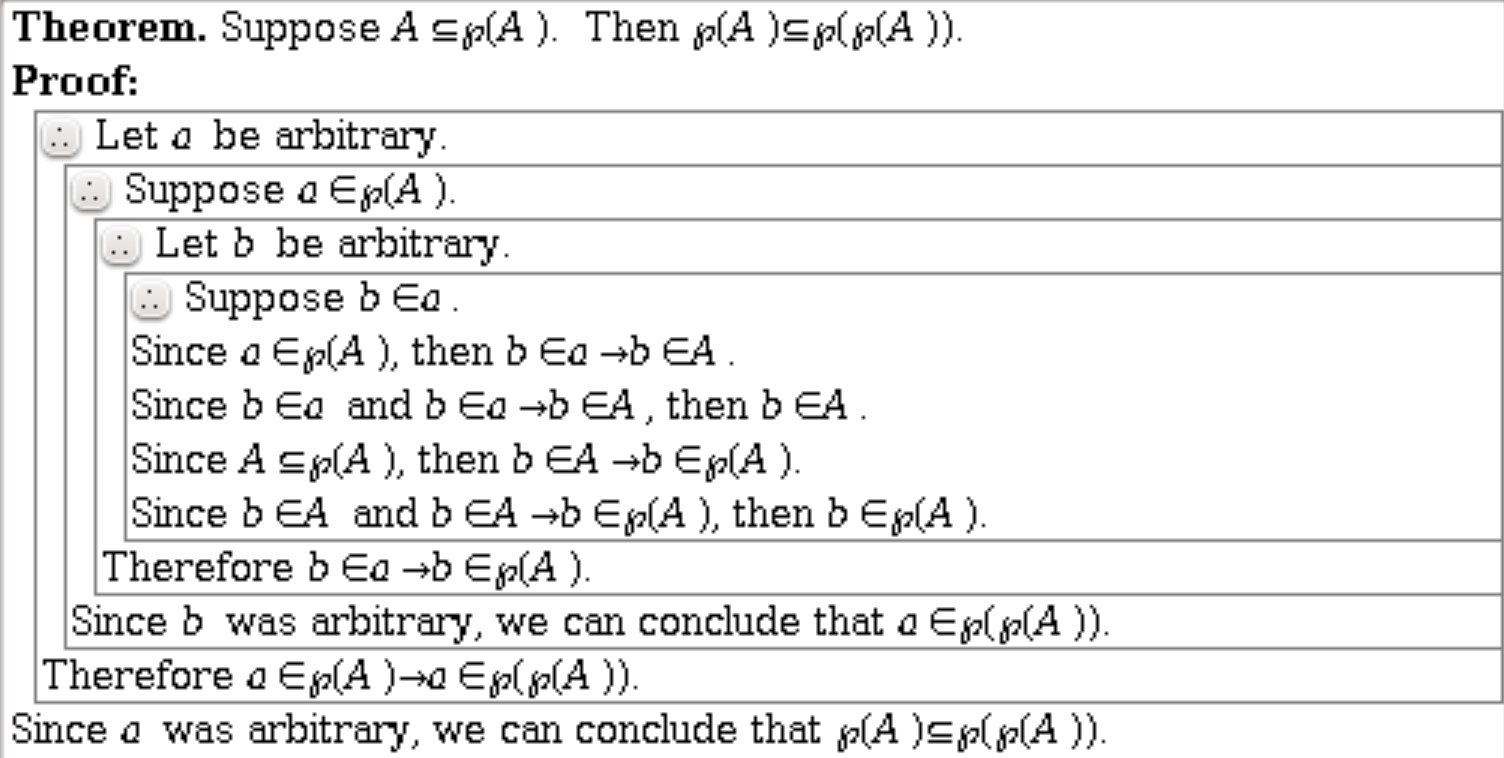
\includegraphics[width=\textwidth]{3_3_4}

\vspace{30pt}

5. The hypothesis of the theorem proven in exercise 4 is $A \subseteq \mathcal{P} (A)$.

\hspace{12pt}(a) Can you think of a set A for which this hypothesis is true?

\hspace{12pt}(b) Can you think of another?
\vspace{30pt}

(a) $A = \{3, 4\}$

$\mathcal{P} (A) = \{\varnothing, \{3\}, \{4\}, \{3, 4\}\}$

\vspace{20pt}

(b) $\mathcal{P} (A) \subseteq \mathcal{P} (\mathcal{P} (A))$

$A = \{3\}$

$\mathcal{P} (A) = \{\varnothing, \{3\}\}$

$\mathcal{P} (\{\varnothing, \{3\}\}) = \{\varnothing, \{\varnothing\}, \{3\}, \{\varnothing, \{3\}\}$

\vspace{30pt}

6. Suppose x is a real number.

\hspace{12pt}(a) Prove that if $x \neq 1$ then there is a real number y such that $\frac{y+1}{y-2} = x$.

\hspace{12pt}(b) Prove that if there is a real number y such that $\frac{y+1}{y-2} = x$, then $x \neq 1$.
\vspace{30pt}

(a)

\centerline{
  \begin{tabular}{l l}
  \textit{Givens} & \textit{Goal} \\
    $x \neq 1$ & $\exists y (\frac{y+1}{y-2} = x)$ \\
  \end{tabular}}
\vspace{10pt}

\textbf{Theorem.} \textit{If $x \neq 1$ then there is a real number y such that $\frac{y+1}{y-2} = x$}

\textit{Proof.}

Let $y = 5$

\quad $\frac{y+1}{y-2} = x$, it follows that $x = 2$.

Thus, $\exists y (\frac{y+1}{y-2} = x)$


\vspace{20pt}

(b)

\centerline{
  \begin{tabular}{l l}
  \textit{Givens} & \textit{Goal} \\
    $\exists y (\frac{y+1}{y-2} = x)$ & $x \neq 1$ \\
  \end{tabular}}
\vspace{10pt}

$$x = 1$$
$$0*y = 3$$
$$y = \frac{3}{0}$$

y is undefined, which contradicts the given $\exists y (\frac{y+1}{y-2} = x)$

\textbf{Theorem.} If there is a real number y such that $\frac{y+1}{y-2} = x$, then $x \neq 1$.

\textit{Proof.} Suppose x = 1. Since $\frac{y+1}{y-2} = x$ and $x = 1$, it follows that $y = \frac{3}{0}$.
It means that y is undefined which contradicts the given $\exists y (\frac{y+1}{y-2} = x)$. Thus, $x \neq 1$.

\vspace{30pt}

*7. Prove that for every real number x, if $x > 2$ then there is a real number
y such that $y + \frac{1}{y} = x$.
\vspace{30pt}

\centerline{
  \begin{tabular}{l l}
  \textit{Givens} & \textit{Goal} \\
    & $\forall x (x > 2 \to \exists y (y + \frac{1}{y} = x)$ \\
  \end{tabular}}
\vspace{10pt}

\centerline{
  \begin{tabular}{l l}
  \textit{Givens} & \textit{Goal} \\
    $x > 2$ & $\exists y (y + \frac{1}{y} = x)$ \\
  \end{tabular}}
\vspace{10pt}

$$y + \frac{1}{y} = x$$
$$y^2 - xy + 1 = 0$$
$$D = x^2 - 4$$
$$y_0 = \frac{x+\sqrt{x^2-4}}{2}$$
$$y_1 = \frac{x-\sqrt{x^2-4}}{2}$$

\textbf{Theorem.} For every real number x, if $x > 2$ then there is a real number
y such that $y + \frac{1}{y} = x$.

\textit{Proof.} Suppose $x > 2$. Let $y = \frac{x+\sqrt{x^2-4}}{2}$, which is defined since $x^2 - 4 > 0$. Then
$y+\frac{1}{y} = \frac{x+\sqrt{x^2-4}}{2} + \frac{2}{x+\sqrt{x^2-4}} = \frac{(x+\sqrt{x^2-4})^2 + 4}{2(x+\sqrt{x^2-4})} = \frac{x^2 + x^2 - 4 + 2x\sqrt{x^2-4} + 4}{2(x+\sqrt{x^2-4})} = \frac{2x(x + \sqrt{x^2-4})}{2(x+\sqrt{x^2-4})} = x$

\vspace{30pt}

$^{\textit{P}}_{\, \textit{D}}$ 8. Prove that if $\mathcal{F}$ is a family of sets and $A \in \mathcal{F}$, then $A \subseteq \cup \mathcal{F}$.
\vspace{30pt}

\textbf{3.3.8.pd}
\vspace{10pt}

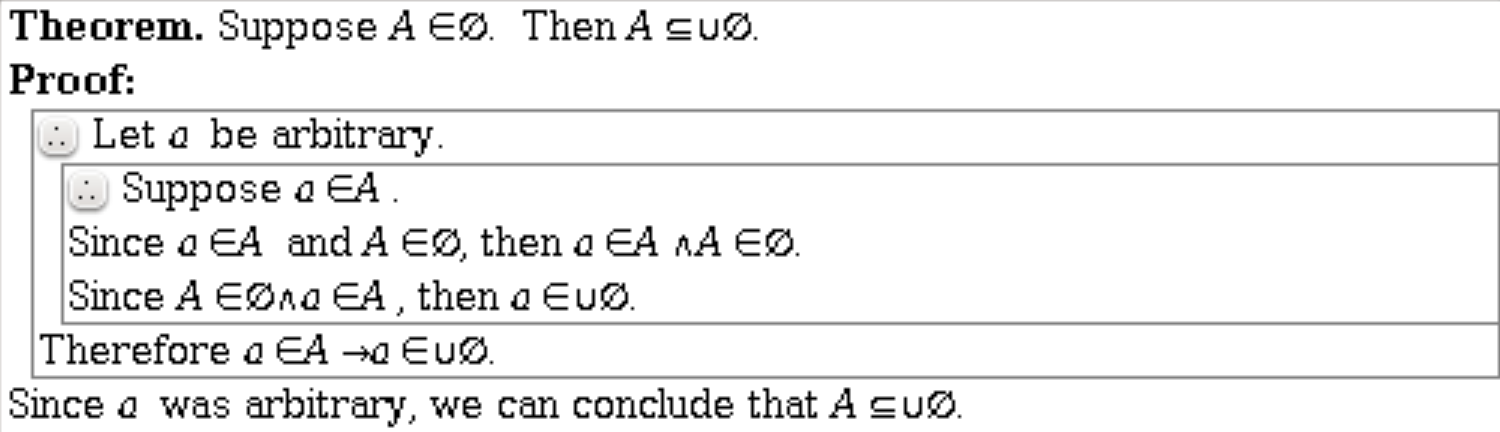
\includegraphics[width=\textwidth]{3_3_8}

\vspace{30pt}

*9. Prove that if $\mathcal{F}$ is a family of sets and $A \in \mathcal{F}$, then $\cap \mathcal{F} \subseteq A$.
\vspace{30pt}

\centerline{
  \begin{tabular}{l l}
  \textit{Givens} & \textit{Goal} \\
    $A \in \mathcal{F}$ & $\cap \mathcal{F} \subseteq A$ \\
  \end{tabular}}
\vspace{10pt}

$$\cap \mathcal{F} \subseteq A$$
$$\forall B (B \in \cap \mathcal{F} \to B \in A)$$
$$\forall B (\forall C (C \in \mathcal{F} \to B \in C) \to B \in A)$$

1) Let B be arbitrary set.

2) $\forall C (C \in \mathcal{F} \to B \in C) \to B \in A$

3) Direct.

\centerline{
  \begin{tabular}{l l}
  \textit{Givens} & \textit{Goal} \\
    $A \in \mathcal{F}$ & $B \in A$ \\
    $\forall C (C \in \mathcal{F} \to B \in C)$ & \\
  \end{tabular}}
\vspace{10pt}

4) Universal instantiation

\centerline{
  \begin{tabular}{l l}
  \textit{Givens} & \textit{Goal} \\
    $B \in A$ & $B \in A$ \\
  \end{tabular}}
\vspace{10pt}

Proved.

\textbf{Theorem.} If $\mathcal{F}$ is a family of sets and $A \in \mathcal{F}$, then $\cap \mathcal{F} \subseteq A$.

\textit{Proof.}

Suppose $\mathcal{F}$ is a family of sets and $A \in \mathcal{F}$

\quad Let B be arbitrary set.

\quad \quad Let $\forall C (C \in \mathcal{F} \to B \in C)$.

\quad \quad \quad Since $\forall C (C \in \mathcal{F} \to B \in C)$ and $A \in \mathcal{F}$,

\quad \quad \quad it follows $B \in A$

\quad \quad Thus, $B \in A$

\quad Since B was arbitrary set, thus $\forall B (B \in \cap \mathcal{F} \to B \in A)$.

Therefore, $\cap \mathcal{F} \subseteq A$.

\vspace{30pt}

10. Suppose that $\mathcal{F}$ is a nonempty family of sets, B is a set, and $\forall A \in \mathcal{F}(B \subseteq A)$. Prove that $B \subseteq \cap \mathcal{F}$.
\vspace{30pt}

\centerline{
  \begin{tabular}{l l}
  \textit{Givens} & \textit{Goal} \\
    $\forall A \in \mathcal{F}(B \subseteq A)$ & $B \subseteq \cap \mathcal{F}$ \\
  \end{tabular}}
\vspace{10pt}

$B \subseteq \cap \mathcal{F}$

$\forall C (C \in B \to C \in \cap \mathcal{F})$

1) Let C be arbitrary set. Then $C \in B \to C \in \cap \mathcal{F}$

2) Suppose $C \in B$.

$C \in \cap \mathcal{F}$

$\forall D (D \in \mathcal{F} \to C \in D)$

3) Let D be arbitrary set. Then $D \in \mathcal{F} \to C \in D$

4) Suppose $D \in \mathcal{F}$.

\centerline{
  \begin{tabular}{l l}
  \textit{Givens} & \textit{Goal} \\
    $\forall A \in \mathcal{F}(B \subseteq A)$ & $C \in D$ \\
    $C \in B$ & \\
    $D \in \mathcal{F}$ & \\
  \end{tabular}}
\vspace{10pt}

5) Universal instantiation

\centerline{
  \begin{tabular}{l l}
  \textit{Givens} & \textit{Goal} \\
    $B \subseteq D$ & $C \in D$ \\
    $C \in B$ & \\
  \end{tabular}}
\vspace{10pt}

\centerline{
  \begin{tabular}{l l}
  \textit{Givens} & \textit{Goal} \\
    $\forall E (E \in B \to E \in D)$ & $C \in D$ \\
    $C \in B$ & \\
  \end{tabular}}
\vspace{10pt}

6) Universal instantiation.

\centerline{
  \begin{tabular}{l l}
  \textit{Givens} & \textit{Goal} \\
    $C \in D$ & $C \in D$ \\
  \end{tabular}}
\vspace{10pt}

Proved.
\vspace{20pt}

\textbf{Theorem.} Suppose that $\mathcal{F}$ is a nonempty family of sets, B is a set, and $\forall A \in \mathcal{F}(B \subseteq A)$. Then $B \subseteq \cap \mathcal{F}$.

\textit{Proof.}

Suppose that $\mathcal{F}$ is a nonempty family of sets, B is a set, and $\forall A \in \mathcal{F}(B \subseteq A)$

\quad Let C be arbitrary set. Then $C \in B \to C \in \cap \mathcal{F}$

\quad \quad Suppose $C \in B$.

\quad \quad $C \in \cap \mathcal{F}$ is equivalent to $\forall D (D \in \mathcal{F} \to C \in D)$

\quad \quad \quad Let D be arbitrary set.

\quad \quad \quad \quad Suppose $D \in \mathcal{F}$

\quad \quad \quad \quad \quad Since $D \in \mathcal{F}$ and $\forall A \in \mathcal{F}(B \subseteq A)$, it follows that $B \subseteq D$.

\quad \quad \quad \quad \quad Since $B \subseteq D$ and $C \in B$, it follows that $C \in D$. 

\quad \quad \quad \quad Thus $D \in \mathcal{F} \to C \in D$.

\quad \quad \quad Since D was arbitrary set, thus $\forall D (D \in \mathcal{F} \to C \in D)$

\quad \quad Thus $C \in \cap \mathcal{F}$

\quad Since C was arbitrary set, thus $\forall C (C \in B \to C \in \cap \mathcal{F})$

Therefore, $B \subseteq \cap \mathcal{F}$.

\vspace{30pt}

\vspace{30pt}

11. Suppose that $\mathcal{F}$ is a family of sets. Prove that if $\varnothing \in \mathcal{F}$ then $\cap \mathcal{F} = \varnothing$.
\vspace{30pt}

\centerline{
  \begin{tabular}{l l}
  \textit{Givens} & \textit{Goal} \\
    $\varnothing \in \mathcal{F}$ & $\cap \mathcal{F} = \varnothing$ \\
  \end{tabular}}
\vspace{10pt}

$\mathcal{F} = \{A_i \mid i \in I\}$

$\cap \mathcal{F} = \{x \mid \forall i \in I (x \in A_i)\}$
\vspace{10pt}

\textbf{Theorem.} Suppose that $\mathcal{F}$ is a family of sets. If $\varnothing \in \mathcal{F}$ then $\cap \mathcal{F} = \varnothing$.

\textit{Proof.} Suppose $\varnothing \in \mathcal{F}$. Since $\mathcal{F} = \{A_i \mid i \in I\}$ and $\varnothing \in \mathcal{F}$, it means that one element in the $\mathcal{F}$ equals $\varnothing$. Since $\cap \mathcal{F} = \cap_{i \in I}A_i$ and one equals $\varnothing$, it follows that $\cap \mathcal{F} = \varnothing \cap \dots = x \in \varnothing \land \dots = \varnothing$. Thus, $\cap \mathcal{F} = \varnothing$

\vspace{30pt}

$^{\textit{P}}_{\, \textit{D}}$ *12. Suppose $\mathcal{F}$ and $\mathcal{G}$ are families of sets. Prove that if $\mathcal{F} \subseteq \mathcal{G}$ then $\cup \mathcal{F} \subseteq \cup\mathcal{G}$.
\vspace{30pt}

\textbf{3.3.12.pd}
\vspace{10pt}

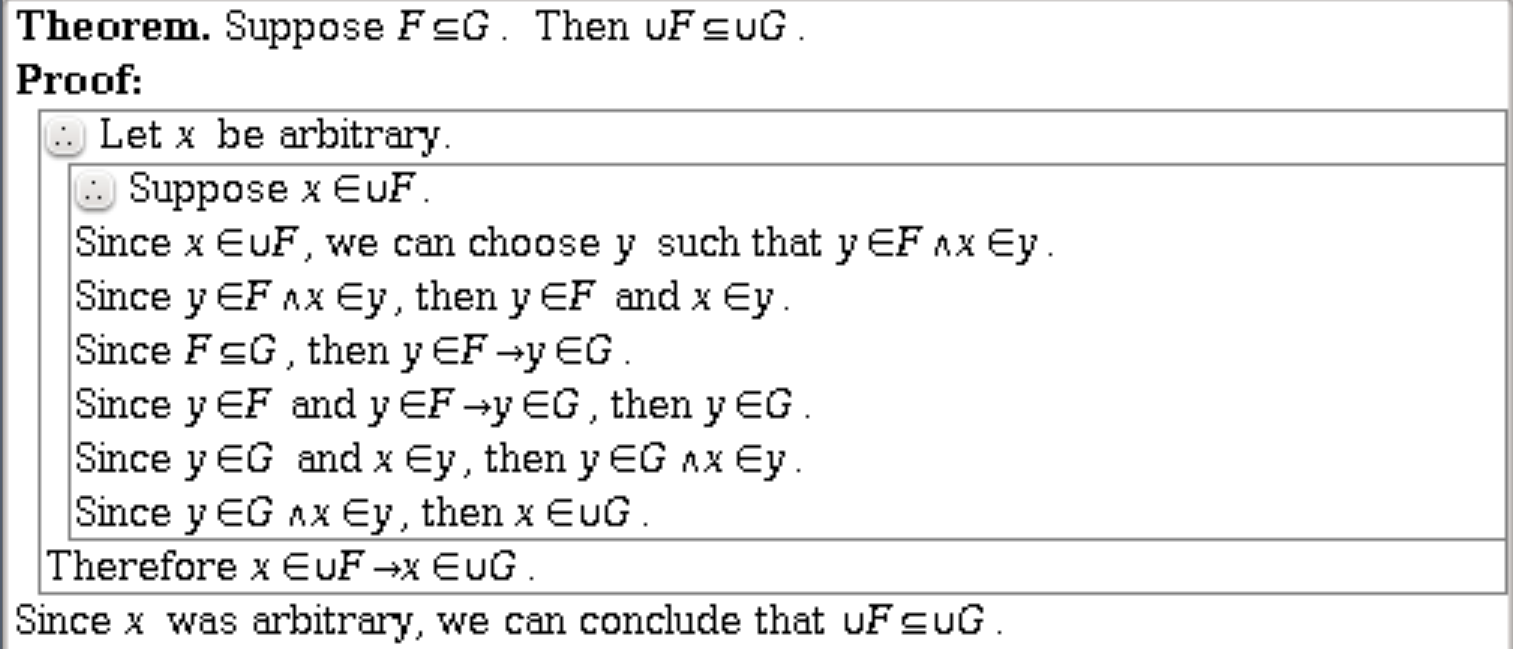
\includegraphics[width=\textwidth]{3_3_12}

\vspace{30pt}

13. Suppose $\mathcal{F}$ and $\mathcal{G}$ are nonempty families of sets. Prove that if $\mathcal{F} \subseteq \mathcal{G}$ then $\cap \mathcal{G} \subseteq \cap\mathcal{F}$.
\vspace{30pt}

\centerline{
  \begin{tabular}{l l}
  \textit{Givens} & \textit{Goal} \\
    $\mathcal{F} \subseteq \mathcal{G}$ & $\cap \mathcal{G} \subseteq \cap\mathcal{F}$. \\
  \end{tabular}}
\vspace{10pt}

$\cap \mathcal{G} \subseteq \cap\mathcal{F}$

$\forall x (x \in \cap \mathcal{G} \to x \in \cap \mathcal{F})$

1) Let x be arbitrary set. Then $x \in \cap \mathcal{G} \to x \in \cap \mathcal{F}$

2) Suppose $x \in \cap \mathcal{G}$

$x \in \cap \mathcal{F}$

$\forall y (y \in \mathcal{F} \to x \in y)$

3) Let y be arbitrary set. Then $y \in \mathcal{F} \to x \in y$

4) Suppose $y \in \mathcal{F}$

\centerline{
  \begin{tabular}{l l}
  \textit{Givens} & \textit{Goal} \\
    $\mathcal{F} \subseteq \mathcal{G}$ & $x \in y$ \\
    $x \in \cap \mathcal{G}$ & \\
    $y \in \mathcal{F}$ & \\
  \end{tabular}}
\vspace{10pt}

$x \in \cap \mathcal{G}$

$\forall z (z \in \mathcal{G} \to x \in z)$

\centerline{
  \begin{tabular}{l l}
  \textit{Givens} & \textit{Goal} \\
    $\mathcal{F} \subseteq \mathcal{G}$ & $x \in y$ \\
    $\forall z (z \in \mathcal{G} \to x \in z)$ & \\
    $y \in \mathcal{F}$ & \\
  \end{tabular}}
\vspace{10pt}

$\mathcal{F} \subseteq \mathcal{G}$

$\forall m (m \in \mathcal{F} \to m \in \mathcal{G})$

\centerline{
  \begin{tabular}{l l}
  \textit{Givens} & \textit{Goal} \\
    $\forall m (m \in \mathcal{F} \to m \in \mathcal{G})$ & $x \in y$ \\
    $\forall z (z \in \mathcal{G} \to x \in z)$ & \\
    $y \in \mathcal{F}$ & \\
  \end{tabular}}
\vspace{10pt}

5) Since $y \in \mathcal{F}$ and $\forall m (m \in \mathcal{F} \to m \in \mathcal{G})$, it follows that
$y \in \mathcal{G}$

6) Since $y \in \mathcal{G}$ and $\forall z (z \in \mathcal{G} \to x \in z)$, it follows that
$x \in y$.

Proved.

\textbf{Theorem.} Suppose $\mathcal{F}$ and $\mathcal{G}$ are nonempty families of sets. If $\mathcal{F} \subseteq \mathcal{G}$ then $\cap \mathcal{G} \subseteq \cap\mathcal{F}$.


\textit{Proof.}

Suppose $\mathcal{F} \subseteq \mathcal{G}$.

\quad Let x be arbitrary set. Then $x \in \cap \mathcal{G} \to x \in \mathcal{F}$

\quad \quad Suppose $x \in \cap \mathcal{G}$

\quad \quad \quad Let y be arbitrary set. Then $y \in \mathcal{F} \to x \in y$

\quad \quad \quad \quad Suppose $y \in \mathcal{F}$

\quad \quad \quad \quad \quad Since $y \in \mathcal{F}$ and $\mathcal{F} \subseteq \mathcal{G}$,
it follows that $y \in \mathcal{G}$

\quad \quad \quad \quad \quad Since $y \in \mathcal{G}$ and $x \in \cap \mathcal{G}$,
it follows that $x \in y$

\quad \quad \quad \quad Thus, $y \in \mathcal{F} \to x \in y$

\quad \quad \quad Since y was arbitrary set, then $\forall y (y \in \mathcal{F} \to x \in y)$

\quad \quad Thus, $x \in \cap \mathcal{G} \to x \in \mathcal{F}$

\quad Since x was arbitrary set, then $\forall x (x \in \cap \mathcal{G} \subseteq x \in \cap \mathcal{F})$

Therefore, $\cap \mathcal{G} \subseteq \cap\mathcal{F}$

\vspace{30pt}

*14. Suppose $\{A_i \mid i \in I\}$ is an indexed family of sets. Prove that
$\cup_{i \in I}\mathcal{P} (A_i) \subseteq \mathcal{P} (\cup_{i \in I} A_i).$ (Hint: First make sure you know what all
the notation means!)
\vspace{30pt}

\centerline{
  \begin{tabular}{l l}
  \textit{Givens} & \textit{Goal} \\
    $$ & $\cup_{i \in I}\mathcal{P} (A_i) \subseteq \mathcal{P} (\cup_{i \in I} A_i)$ \\
  \end{tabular}}
\vspace{10pt}

$\cup_{i \in I}\mathcal{P} (A_i) \subseteq \mathcal{P} (\cup_{i \in I} A_i)$

$\forall a (a \in \cup_{i \in I}\mathcal{P} (A_i) \to a \in \mathcal{P} (\cup_{i \in I} A_i))$

1) Let a be arbitrary. Then $a \in \cup_{i \in I}\mathcal{P} (A_i) \to a \in \mathcal{P} (\cup_{i \in I} A_i)$

2) Suppose $a \in \cup_{i \in I}\mathcal{P} (A_i)$

$a \in \mathcal{P} (\cup_{i \in I} A_i)$

$\forall b (b \in a \to b \in \cup_{i \in I} A_i)$

3) Let b be arbitrary. Then $b \in a \to b \in \cup_{i \in I} A_i$

4) Suppose $b \in a$

\centerline{
  \begin{tabular}{l l}
  \textit{Givens} & \textit{Goal} \\
    $a \in \cup_{i \in I}\mathcal{P} (A_i)$ & $b \in \cup_{i \in I} A_i$ \\
    $b \in a$ & \\
  \end{tabular}}
\vspace{10pt}

$a \in \cup_{i \in I}\mathcal{P} (A_i)$

$\exists i \in I (a \in \mathcal{P}(A_i))$

$\exists i \in I \forall c (c \in a \to c \in A_i)$

$b \in \cup_{i \in I} A_i$

$\exists i \in I (b \in A_i)$

\centerline{
  \begin{tabular}{l l}
  \textit{Givens} & \textit{Goal} \\
    $\exists i \in I \forall c (c \in a \to c \in A_i)$ & $\exists i \in I (b \in A_i)$ \\
    $b \in a$ & \\
  \end{tabular}}
\vspace{10pt}

5) Since $b \in a$ and $\forall c (c \in a \to c \in A_i)$, it follows that $b \in A_i$.
Thus, $\exists i \in I (b \in A_i)$.

Proved.
\vspace{20pt}

\textbf{Theorem.} Suppose $\{A_i \mid i \in I\}$ is an indexed family of sets. Then $\cup_{i \in I}\mathcal{P} (A_i) \subseteq \mathcal{P} (\cup_{i \in I} A_i).$

\textit{Proof.}

Suppose $\{A_i \mid i \in I\}$ is an indexed family of sets.

\quad Let a be arbitrary. Then $a \in \cup_{i \in I}\mathcal{P} (A_i) \to a \in \mathcal{P} (\cup_{i \in I} A_i)$

\quad \quad Suppose $a \in \cup_{i \in I}\mathcal{P} (A_i)$.

\quad \quad \quad Let b be arbitrary. Then $b \in a \to b \in \cup_{i \in I} A_i$

\quad \quad \quad \quad Suppose $b \in A$

\quad \quad \quad \quad \quad $a \in \cup_{i \in I}\mathcal{P} (A_i)$ is $\exists i \in I \forall c (c \in a \to c \in A_i).$

\quad \quad \quad \quad \quad Since $b \in a$ and $\exists i \in I \forall c (c \in a \to c \in A_i)$, it follows that

\quad \quad \quad \quad \quad $\exists i \in I (b \in A_i)$.

\quad \quad \quad \quad Thus, $b \in a \to b \in \cup_{i \in I} A_i$.

\quad \quad \quad Since b was arbitrary, then $\forall b (b \in a \to b \in \cup_{i \in I} A_i)$

\quad \quad Therefore, $a \in \cup_{i \in I}\mathcal{P} (A_i) \to a \in \mathcal{P} (\cup_{i \in I} A_i)$.

\quad Since a was arbitrary, then $\forall a (a \in \cup_{i \in I}\mathcal{P} (A_i) \to a \in \mathcal{P} (\cup_{i \in I} A_i))$.

Therefore, $\cup_{i \in I}\mathcal{P} (A_i) \subseteq \mathcal{P} (\cup_{i \in I} A_i)$.

\vspace{30pt}

15. Suppose $\{A_i \mid i \in I\}$ is an indexed family of sets and $I \neq \varnothing$. Prove that
$\cap_{i \in I} A_i \in \cap_{i \in I} \mathcal{P} (A_i)$.
\vspace{30pt}

\centerline{
  \begin{tabular}{l l}
  \textit{Givens} & \textit{Goal} \\
    $$ & $\cap_{i \in I} A_i \in \cap_{i \in I} \mathcal{P} (A_i)$ \\
  \end{tabular}}
\vspace{10pt}

$\cap_{i \in I} A_i = \forall i \in I (x \in A_i) = a$

$\cap_{i \in I} \mathcal{P} (A_i) = \forall i \in I (a \in \mathcal{P}(A_i))$

$\forall i \in I \forall b (b \in A \to b \in A_i)$

$\forall i \in I \forall b (\forall i \in I (b \in A_i) \to b \in A_i)$

\vspace{20pt}

\textbf{Theorem.} Suppose $\{A_i \mid i \in I\}$ is an indexed family of sets and $I \neq \varnothing$. Then $\cap_{i \in I} A_i \in \cap_{i \in I} \mathcal{P} (A_i)$.

\textit{Proof.}

Let i be arbitrary element from I.

\quad Let b be arbitrary.

\quad \quad Suppose $\forall i \in I (b \in A_i)$

\quad \quad \quad Since $\forall i \in I (b \in A_i)$ and $i \in I$, it follows that $b \in A_i$

\quad \quad Therefore, $\forall i \in I (b \in A_i) \to b \in A_i$

\quad Since b was arbitrary, then $\forall b (\forall i \in I (b \in A_i) \to b \in A_i)$

Since i was arbitrary element from I, then $\forall i \in I \forall b (\forall i \in I (b \in A_i) \to b \in A_i)$.

Therefore, $\cap_{i \in I} A_i \in \cap_{i \in I} \mathcal{P} (A_i)$.

\vspace{30pt}

$^{\textit{P}}_{\, \textit{D}}$ 16. Prove the converse of the statement proven in Example 3.3.5. In other
words, prove that if $\mathcal{F} \subseteq \mathcal{P} (B)$ then $\cup \mathcal{F} \subseteq B$.
\vspace{30pt}

\textbf{3.3.16.pd}
\vspace{10pt}

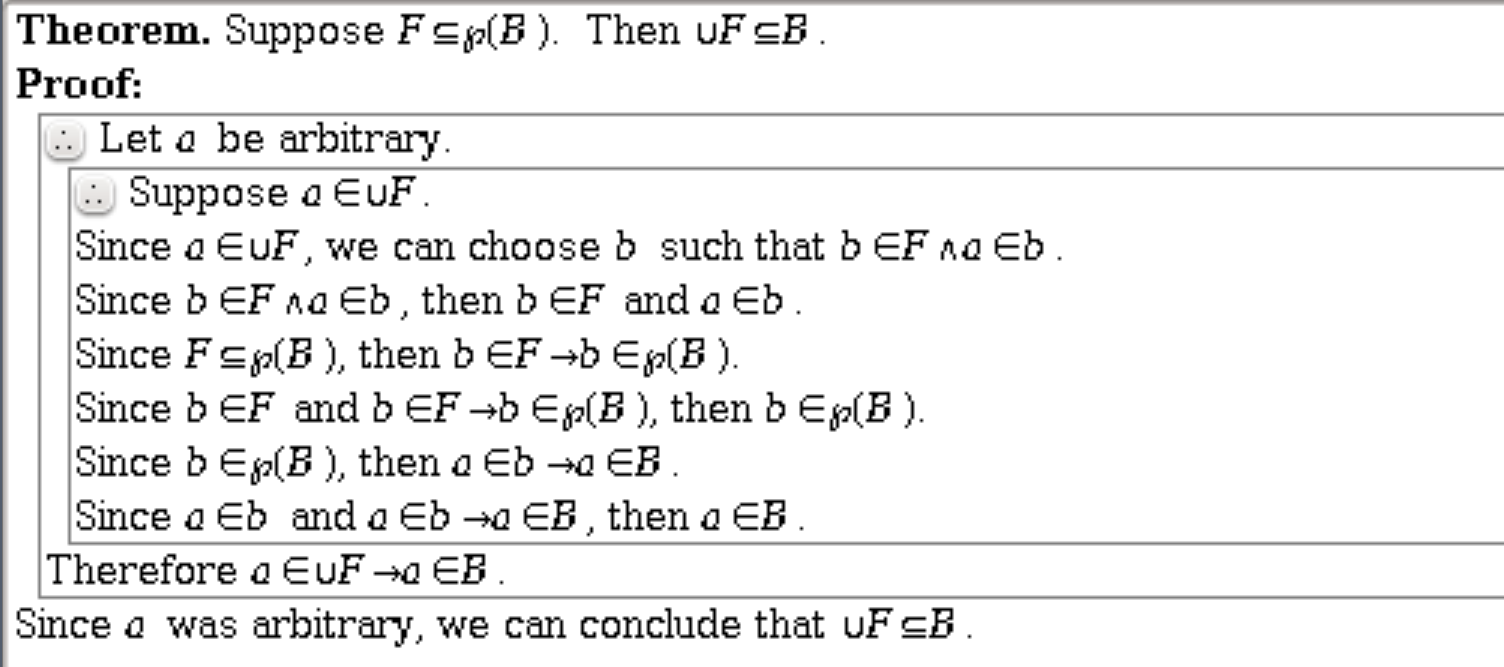
\includegraphics[width=\textwidth]{3_3_16}

\vspace{30pt}

*17. Suppose $\mathcal{F}$ and $\mathcal{G}$ are nonempty families of sets, and every element of
$\mathcal{F}$ is a subset of every element of $\mathcal{G}$. Prove that $\cup \mathcal{F} \subseteq \cap \mathcal{G}$.
\vspace{30pt}

\centerline{
  \begin{tabular}{l l}
  \textit{Givens} & \textit{Goal} \\
    $\forall f \in \mathcal{F} \forall g \in \mathcal{G}(f \subseteq g)$ & $\cup \mathcal{F} \subseteq \cap \mathcal{G}$ \\
  \end{tabular}}
\vspace{10pt}

$\cup \mathcal{F} \subseteq \cap \mathcal{G}$

$\forall a (a \in \cup \mathcal{F} \to a \in \cap \mathcal{G})$

1) Let a be arbitrary. Then $a \in \cup \mathcal{F} \to a \in \cap \mathcal{G}$

2) Suppose $a \in \cup \mathcal{F}$

$a \in \cup \mathcal{F}$

$\exists A (A \in \mathcal{F} \land a \in A)$
\vspace{10pt}

$a \in \cap \mathcal{G}$

$\forall B (B \in \mathcal{G} \to a \in B)$
\vspace{10pt}

\centerline{
  \begin{tabular}{l l}
  \textit{Givens} & \textit{Goal} \\
    $\forall f \in \mathcal{F} \forall g \in \mathcal{G}(f \subseteq g)$ & $\forall B (B \in \mathcal{G} \to a \in B)$ \\
    $\exists A (A \in \mathcal{F} \land a \in A)$ & \\
  \end{tabular}}
\vspace{10pt}

3) Let B be arbitrary. Then $B \in \mathcal{G} \to a \in B$

4) Suppose $B \in \mathcal{G}$.

\centerline{
  \begin{tabular}{l l}
  \textit{Givens} & \textit{Goal} \\
    $\forall f \in \mathcal{F} \forall g \in \mathcal{G}(f \subseteq g)$ & $a \in B$ \\
    $\exists A (A \in \mathcal{F} \land a \in A)$ & \\
    $B \in \mathcal{G}$ & \\
  \end{tabular}}
\vspace{10pt}

5) Since $B \in \mathcal{G}$ and $\forall f \in \mathcal{F} \forall g \in \mathcal{G}(f \subseteq g)$, it follows, $\forall f \in \mathcal{F} (f \subseteq B)$

\centerline{
  \begin{tabular}{l l}
  \textit{Givens} & \textit{Goal} \\
    $\forall f \in \mathcal{F} (f \subseteq B)$ & $a \in B$ \\
    $\exists A (A \in \mathcal{F} \land a \in A)$ & \\
  \end{tabular}}
\vspace{10pt}

6) Since $\exists A (A \in \mathcal{F} \land a \in A)$ we can choose $A = A_0$ such that
$A_0 \in \mathcal{F} \land a \in A_0$.

\centerline{
  \begin{tabular}{l l}
  \textit{Givens} & \textit{Goal} \\
    $\forall f \in \mathcal{F} (f \subseteq B)$ & $a \in B$ \\
    $A_0 \in \mathcal{F}$ & \\
    $a \in A_0$ & \\
  \end{tabular}}
\vspace{10pt}

7) Since $\forall f \in \mathcal{F} (f \subseteq B)$ and $A_0 \in \mathcal{F}$, it follows that
$A_0 \subseteq B$

\centerline{
  \begin{tabular}{l l}
  \textit{Givens} & \textit{Goal} \\
    $A_0 \subseteq B$ & $a \in B$ \\
    $a \in A_0$ & \\
  \end{tabular}}
\vspace{10pt}

$A_0 \subseteq B$

$\forall c (c \in A_0 \to c \in B)$

\centerline{
  \begin{tabular}{l l}
  \textit{Givens} & \textit{Goal} \\
    $\forall c (c \in A_0 \to c \in B)$ & $a \in B$ \\
    $a \in A_0$ & \\
  \end{tabular}}
\vspace{10pt}

8) Since $\forall c (c \in A_0 \to c \in B)$ and $a \in A_0$, it follows that $a \in B$

Proved.

\textbf{Theorem.} Suppose $\mathcal{F}$ and $\mathcal{G}$ are nonempty families of sets, and every element of
$\mathcal{F}$ is a subset of every element of $\mathcal{G}$. Then $\cup \mathcal{F} \subseteq \cap \mathcal{G}$.

\textit{Proof.}

Suppose $\forall f \in \mathcal{F} \forall g \in \mathcal{G}(f \subseteq g)$

\quad Let a be arbitrary.

\quad \quad Suppose $a \in \cup \mathcal{F}$

\quad \quad \quad Let B be arbitrary

\quad \quad \quad \quad Suppose $B \in \mathcal{G}$

\quad \quad \quad \quad \quad Since $B \in \mathcal{G}$ and $\forall f \in \mathcal{F} \forall g \in \mathcal{G}(f \subseteq g)$,

\quad \quad \quad \quad \quad it follows, $\forall f \in \mathcal{F} (f \subseteq B)$

\quad \quad \quad \quad \quad  Since $\exists A (A \in \mathcal{F} \land a \in A)$ we can choose $A = A_0$ 

\quad \quad \quad \quad \quad such that $A_0 \in \mathcal{F} \land a \in A_0$.

\quad \quad \quad \quad \quad Since $\forall f \in \mathcal{F} (f \subseteq B)$ and $A_0 \in \mathcal{F}$, it follows that $A_0 \subseteq B$

\quad \quad \quad \quad \quad Since $\forall c (c \in A_0 \to c \in B)$ and $a \in A_0$, it follows that $a \in B$

\quad \quad \quad \quad Thus, $B \in \mathcal{G} \to a \in B$.

\quad \quad \quad Since B was arbitrary, thus $\forall B (B \in \mathcal{G} \to a \in B)$

\quad \quad Thus $a \in \cup \mathcal{F} \to a \in \cap \mathcal{G}$.

\quad Since a was arbitrary, thus $\forall a (a \in \cup \mathcal{F} \to a \in \cap \mathcal{G})$.

Therefore, $\cup \mathcal{F} \subseteq \cap \mathcal{G}$

\vspace{30pt}

18. In this problem all variables range over $\mathbb{Z}$, the set of all integers.

\hspace{12pt}(a) Prove that if $a \mid b$ and $a \mid c$, then $a \mid (b + c)$.

\hspace{12pt}(b) Prove that if $ac \mid bc$ and $c \neq 0$, then $a \mid b$.
\vspace{30pt}

(a) 

\centerline{
  \begin{tabular}{l l}
  \textit{Givens} & \textit{Goal} \\
    $a \mid b$ & $a \mid (b + c)$ \\
    $a \mid c$ & \\
  \end{tabular}}
\vspace{10pt}

\centerline{
  \begin{tabular}{l l}
  \textit{Givens} & \textit{Goal} \\
    $ma = b$ & $ka = b + c$ \\
    $na = c$ & \
  \end{tabular}}
\vspace{10pt}

$ka = ma + na$

$ka = a(m + n)$

$k = m + n$

\textbf{Theorem.} If $a \mid b$ and $a \mid c$, then $a \mid (b + c)$.

\textit{Proof.} Let a, b, and c be arbitrary integers and suppose $a \mid b$ and $a \mid c$.
Since $a \mid b$, we can choose some integer m such that $ma = b$. Similarly, since $a \mid c$,
we can choose an integer n such that $na = c$. Therefore $b + c = a(m + n)$, so since $m + n$ is
an integer, $a \mid (b + c)$.

\vspace{20pt}

(b)


\centerline{
  \begin{tabular}{l l}
  \textit{Givens} & \textit{Goal} \\
    $ac \mid bc$ & $a \mid b$ \\
    $c \neq 0$ & \\
  \end{tabular}}
\vspace{10pt}

\centerline{
  \begin{tabular}{l l}
  \textit{Givens} & \textit{Goal} \\
    $mac = bc$ & $a \mid b$ \\
    $c \neq 0$ & \\
  \end{tabular}}
\vspace{10pt}

$mac = bc$

$ma = b$

\textbf{Theorem.} If $ac \mid bc$ and $c \neq 0$ then $a \mid b$

\textit{Proof.} Let a, b, and c be arbitrary integers and suppose $ac \mid bc$ and $c \neq 0$. Since $ac \mid bc$, we can choose some integer m such that $mac = bc$. Since $mac = bc$ and $c \neq 0$, we can conclude $ma = b$. Since $ma = b$ and m is an integer, $a \mid b$.

\vspace{30pt}

19. (a) Prove that for all real numbers x and y there is a real number z such
that $x + z = y - z$.

\hspace{12pt}(b) Would the statement in part (a) be correct if "real number" were
changed to "integer"? Justify your answer.
\vspace{30pt}

(a) $\forall x \in \mathbb{R} \forall y \in \mathbb{R} \exists z \in \mathbb{R} (x + z = y - z)$

1) Let x and y be arbitrary real numbers


\centerline{
  \begin{tabular}{l l}
  \textit{Givens} & \textit{Goal} \\
    $$ & $\exists z \in \mathbb{R} (x + z = y - z)$ \\
  \end{tabular}}
\vspace{10pt}

$x + z = y - z$

$2z = y - x$

$z = \frac{y - x}{2}$

\textbf{Theorem.} For all real numbers x and y there is a real number z such
that $x + z = y - z$.

\textit{Proof.} Let x and y be arbitrary real numbers. Let $z = \frac{y - x}{2}$. $z$ is a real number, since x, y and 2 are all real numbers, then:

\centerline{$x + z = y - z$}

\centerline{$x + \frac{y - x}{2} = y - \frac{y - x}{2}$}

\centerline{$\frac{x + y - x}{2} = \frac{y - y + x}{2}$}

\centerline{$\frac{y}{2} = \frac{x}{2}$}

\centerline{$x = y$}

Thus $\exists z \in \mathbb{R} (x + z = y - z)$.

\vspace{20pt}

(b) No, since we can't prove that $z = \frac{y - x}{2}$ is an integer.
For instance, let $y = 4$ and $x = 1$, so $z = \frac{4-1}{2} = 1.5$ which is real number, but not an integer.


\vspace{30pt}

*20. Consider the following theorem:

\textbf{Theorem.} For every real number x, $x^2 \geq 0$.

What's wrong with the following proof of the theorem?

\textit{Proof.} Suppose not. Then for every real number x, $x^2 < 0$. In particular,
plugging in $x = 3$ we would get $9 < 0$, which is clearly false. This
contradiction shows that for every number x, $x^2 \geq 0$.
\vspace{30pt}

$\forall x \in \mathbb{R} (x^2 \geq 0)$

$\neg \forall x \in \mathbb{R} (x^2 \geq 0)$

$\exists x \in \mathbb{R} (x^2 < 0)$

2nd sentence is wrong. Should be: then there exists real number x such that $x^2 < 0$. Proof is incorrect.

\vspace{30pt}

21. Consider the following incorrect theorem:

\textbf{Incorrect Theorem.} If $\forall x \in A(x \neq 0)$ and $A \subseteq B$ then $\forall x \in B(x
\neq 0)$.

\hspace{12pt}(a) What's wrong with the following proof of the theorem?

\textit{Proof.} Let x be an arbitrary element of A. Since $\forall x \in A(x \neq 0)$,
we can conclude that $x \neq 0$. Also, since $A \subseteq B$, $x \in B$. Since
$x \in B$, $x \neq 0$, and x was arbitrary, we can conclude that $\forall x \in
B(x \neq 0)$.

\hspace{12pt}(b) Find a counterexample to the theorem. In other words, find an example
of sets A and B for which the hypotheses of the theorem are
true but the conclusion is false.
\vspace{30pt}

(a) Last sentence definitely wrong: x was arbitrary element of A and in the last sentence we have the conclusion "x was arbitrary, we can conclude that $\forall x \in B(x \neq 0)$".

\vspace{20pt}

(b) $A = \{1,2,3\}$

$B = \{0,1,2,3\}$

\vspace{30pt}

*22. Consider the following incorrect theorem:

\textbf{Incorrect Theorem.} $\exists x \in \mathbb{R} \forall y \in \mathbb{R}(x y^2 = y - x)$.
What's wrong with the following proof of the theorem?

\textit{Proof.} Let $x = y/(y^2 + 1)$. Then

$y - x = y - \frac{y}{y^2 + 1} = \frac{y^3}{y^2 + 1} = \frac{y}{y^2 + 1} * y^2 = x y^2$
\vspace{30pt}

$\exists x \in \mathbb{R} \forall y \in \mathbb{R}(x y^2 = y - x)$

The proof shoud go like that: let $x = \dots$. Let y be an arbitrary real number...

So, there is no way to declare x in terms of y, since y is defined after x.

\vspace{30pt}

23. Consider the following incorrect theorem:

\textbf{Incorrect Theorem.} Suppose $\mathcal{F}$ and $\mathcal{G}$ are families of sets. If $\cup \mathcal{F}$ and $\cup \mathcal{G}$ are disjoint, then so are $\mathcal{F}$ and $\mathcal{G}$.

\hspace{12pt}(a) What's wrong with the following proof of the theorem?

\textit{Proof.} Suppose $\cup \mathcal{F}$ and $\cup \mathcal{G}$ are disjoint. Suppose $\mathcal{F}$ and $\mathcal{G}$ are not disjoint. Then we can choose some set A such that $A \in \mathcal{F}$ and $A \in \mathcal{G}$.
Since $A \in \mathcal{F}$, by exercise 8, $A \subseteq \cup\mathcal{F}$, so every element of A is in
$\cup \mathcal{F}$. Similarly, since $A \in \mathcal{G}$, every element of A is in $\cup \mathcal{G}$. But then every element of A is in both $\cup \mathcal{F}$ and $\cup \mathcal{G}$, and this is impossible since
$\cup \mathcal{F}$ and $\cup \mathcal{G}$ are disjoint. Thus, we have reached a contradiction, so
$\mathcal{F}$ and $\mathcal{G}$ must be disjoint.

\hspace{12pt}(b) Find a counterexample to the theorem.
\vspace{30pt}

(a) 

\centerline{
  \begin{tabular}{l l}
  \textit{Givens} & \textit{Goal} \\
    $\cup \mathcal{F} \cap \cup \mathcal{G} = \varnothing$ & $\mathcal{F} \cap \mathcal{G} = \varnothing$ \\
  \end{tabular}}
\vspace{10pt}

\centerline{
  \begin{tabular}{l l}
  \textit{Givens} & \textit{Goal} \\
    $\cup \mathcal{F} \cap \cup \mathcal{G} = \varnothing$ & $\neg \exists y (y \in \mathcal{F} \land y \in \mathcal{G})$ \\
  \end{tabular}}
\vspace{10pt}

\centerline{
  \begin{tabular}{l l}
  \textit{Givens} & \textit{Goal} \\
    $\cup \mathcal{F} \cap \cup \mathcal{G} = \varnothing$ & Contradiction \\
    $\exists y (y \in \mathcal{F} \land y \in \mathcal{G})$    
  \end{tabular}}
\vspace{10pt}

\centerline{
  \begin{tabular}{l l}
  \textit{Givens} & \textit{Goal} \\
    $\exists y (y \in \mathcal{F} \land y \in \mathcal{G})$ & $\exists x (x \in \cup \mathcal{F} \land x \in \cup \mathcal{G})$ \\
  \end{tabular}}
\vspace{10pt}

\centerline{
  \begin{tabular}{l l}
  \textit{Givens} & \textit{Goal} \\
    $y_0 \subseteq \cup \mathcal{F} \land y_0 \subseteq \cup \mathcal{G}$ & $\exists x (x \in \cup \mathcal{F} \land x \in \cup \mathcal{G})$ \\
  \end{tabular}}
\vspace{10pt}

\centerline{
  \begin{tabular}{l l}
  \textit{Givens} & \textit{Goal} \\
    $\forall a (a \in y_0 \to a \in \cup \mathcal{F}) \land \forall a (a \in y_0 \to a \in \cup \mathcal{G})$ & $\exists x (x \in \cup \mathcal{F} \land x \in \cup \mathcal{G})$ \\
  \end{tabular}}
\vspace{10pt}

\centerline{
  \begin{tabular}{l l}
  \textit{Givens} & \textit{Goal} \\
    $\forall a ((a \in y_0 \to a \in \cup \mathcal{F}) \land (a \in y_0 \to a \in \cup \mathcal{G}))$ & $\exists x (x \in \cup \mathcal{F} \land x \in \cup \mathcal{G})$ \\
  \end{tabular}}
\vspace{10pt}

\centerline{
  \begin{tabular}{l l}
  \textit{Givens} & \textit{Goal} \\
    $\forall a (a \in y_0 \to (a \in \cup \mathcal{F} \land a \in \cup \mathcal{G}))$ & $\exists x (x \in \cup \mathcal{F} \land x \in \cup \mathcal{G})$ \\
  \end{tabular}}
\vspace{10pt}

Let $A = \varnothing$ and A is both in $\cup \mathcal{F}$ and $\cup \mathcal{G}$, but \textit{this doesn't contradict that the sets are disjoint} (in order to contradict it A should contain an element).

\vspace{20pt}

(b) $\mathcal{F} = \{\{3\}, \{\varnothing\}\}$

$\mathcal{G} = \{\{2\},\{\varnothing\}\}$

$\cup \mathcal{F} = \{3\}$

$\cup \mathcal{G} = \{2\}$

\vspace{30pt}

24. Consider the following putative theorem:

\textbf{Theorem?} For all real numbers x and y, $x^2 + x y - 2y^2 = 0$.

\hspace{12pt}(a) What's wrong with the following proof of the theorem?

\textit{Proof.} Let x and y be equal to some arbitrary real number r. Then
$$x^2 + x y - 2y^2 = r^2 + r * r - 2r^2 = 0$$.
Since x and y were both arbitrary, this shows that for all real numbers
x and y, $x^2 + x y - 2y^2 = 0$.

\hspace{12pt}(b) Is the theorem correct? Justify your answer with either a proof or a
counterexample.
\vspace{30pt}

(a)

The theorem and proof are incorrect. Since $\forall x \forall y (x^2 + x y - 2y^2 = 0)$ the proof should have the form: let x and b be arbitrary real numbers $\dots$

\vspace{20pt}

(b) $x = 1$

$y = 2$

$1 + 2 - 8 \neq 0$

$-5 \neq 0$

\vspace{30pt}

*25. Prove that for every real number x there is a real number y such that for
every real number $z, yz = (x + z)^2 - (x^2 + z^2)$.
\vspace{30pt}

\centerline{
  \begin{tabular}{l l}
  \textit{Givens} & \textit{Goal} \\
    $$ & $\forall x \exists y \forall z (yz = (x + z)^2 - (x^2 + z^2))$ \\
  \end{tabular}}
\vspace{10pt}

$yz = (x + z)^2 - (x^2 + z^2)$

$yz = x^2 + 2xz + z^2 - x^2 - z^2$

$yz = 2xz$

$y = 2x$

\textbf{Theorem.} For every real number x there is a real number y such that for
every real number $z, yz = (x + z)^2 - (x^2 + z^2)$.

\textit{Proof.} Let x be an arbitrary real number. Let $y = 2x$. Let z be an arbitrary real number.

Then:

$yz = (x + z)^2 - (x^2 + z^2)$

$yz = x^2 + 2xz + z^2 - x^2 - z^2$

$yz = 2xz$

$2xz = 2xz$

\vspace{30pt}

26. (a) Comparing the various rules for dealing with quantifiers in proofs,
you should see a similarity between the rules for goals of the form
$\forall x P(x)$ and givens of the form $\exists x P(x)$. What is this similarity?
What about the rules for goals of the form $\exists x P(x)$ and givens of the
form $\forall x P(x)$?

\hspace{12pt}(b) Can you think of a reason why these similarities might be expected?
(Hint: Think about how proof by contradiction works when the goal
starts with a quantifier.)
\vspace{30pt}

(a) The goals of the form $\forall x P(x)$ and the givens of the form $\exists x P(x)$:
you don't get to choose a particular value to plug in for x.

The goals of the form $\exists x P(x)$ and the givens of the form $\forall x P(x)$:
you can choose a particular value to plug in for x.

\vspace{20pt}

(b)

These similarities might be expected since:

a) negation of the $\forall x P(x)$ goal gives:

$\neg \forall x P(x)$

$\exists x \neg P(x)$

So, "moving" the goal of the form $\forall x P(x)$ to givens we get $\exists x \neg P(x)$

\vspace{10pt}
b) negation of the $\exists x P(x)$ goal gives:

$\neg \exists x P(x)$

$\forall x \neg P(x)$

So, "moving" the goal of the form $\exists x P(x)$ to givens we get $\forall x \neg P(x)$

\vspace{50pt}

\textbf{3.4. Proofs Involving Conjunctions and Biconditionals}

Exercises
\vspace{30pt}

*1. Use the methods of this chapter to prove that $\forall x(P(x) \land Q(x))$ is
equivalent to $\forall x P(x) \land \forall x Q(x)$.
\vspace{30pt}

\textbf{3.4.1.pd}
\vspace{10pt}

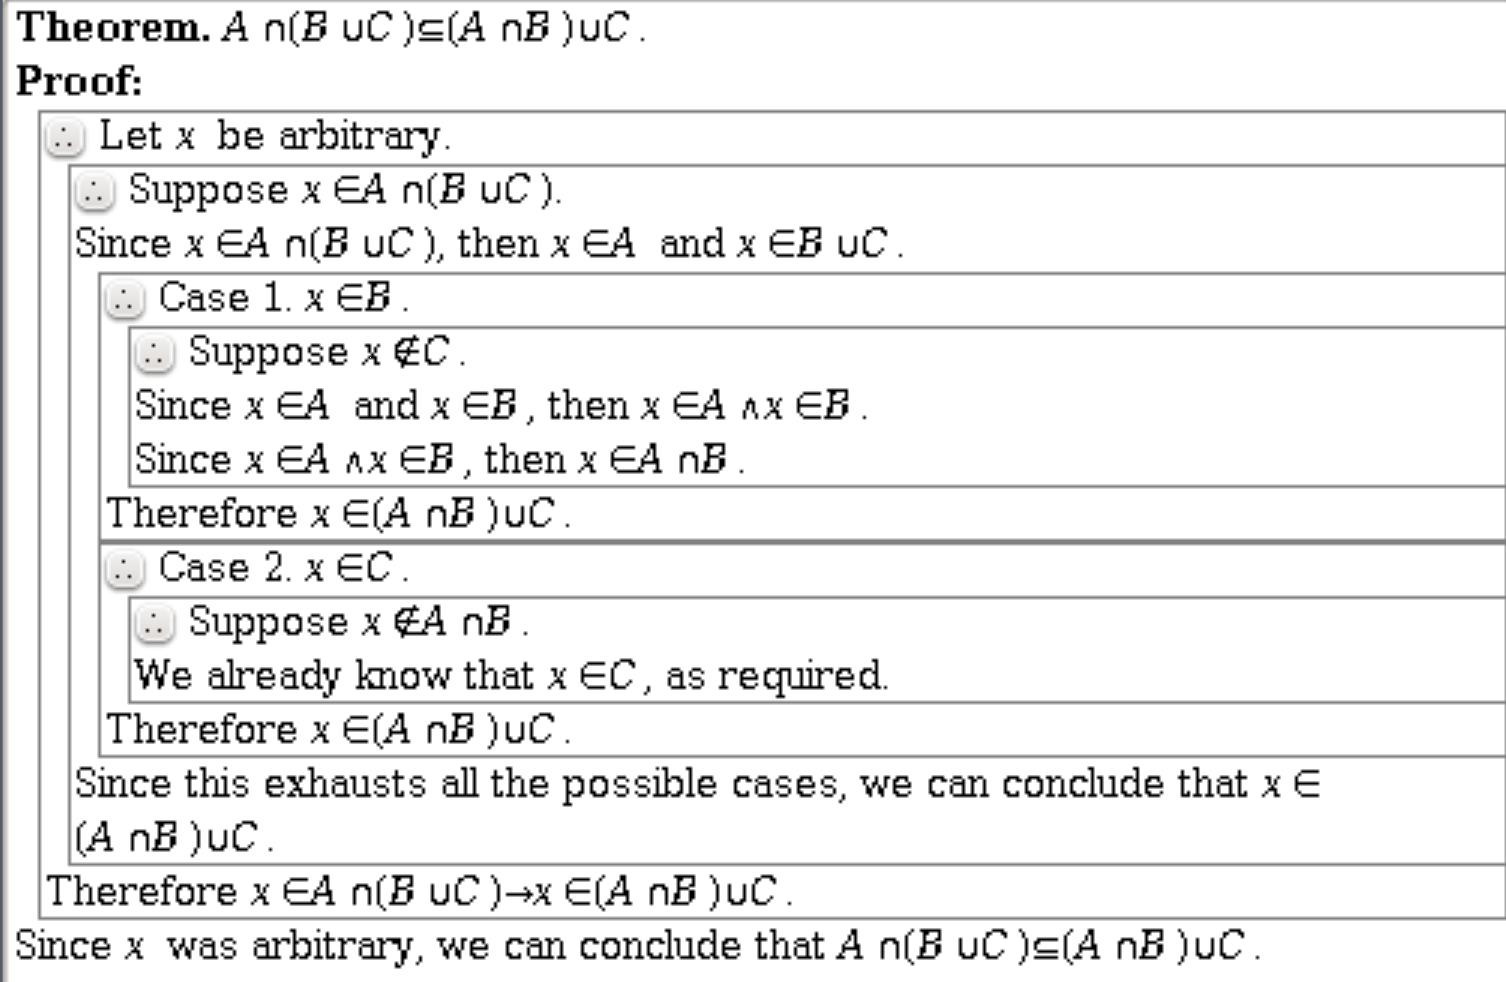
\includegraphics[width=\textwidth]{3_4_1}

\vspace{30pt}

$^{\textit{P}}_{\, \textit{D}}$ 2. Prove that if $A \subseteq B$ and $A \subseteq C$ then $A \subseteq B \cap C$.
\vspace{30pt}

\textbf{3.4.2.pd}
\vspace{10pt}

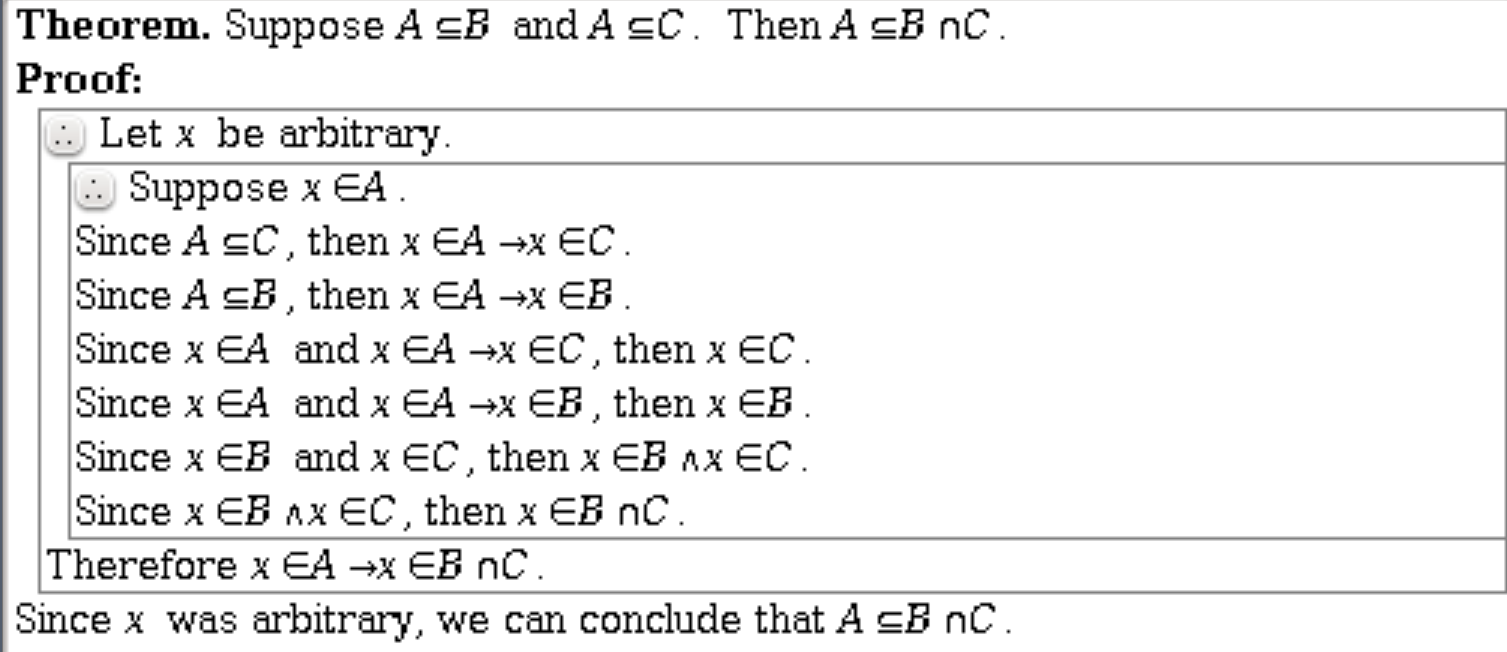
\includegraphics[width=\textwidth]{3_4_2}

\vspace{30pt}

$^{\textit{P}}_{\, \textit{D}}$ 3. Suppose $A \subseteq B$. Prove that for every set C, $C \setminus B \subseteq C \setminus A$.
\vspace{30pt}

\textbf{3.4.3.pd}
\vspace{10pt}

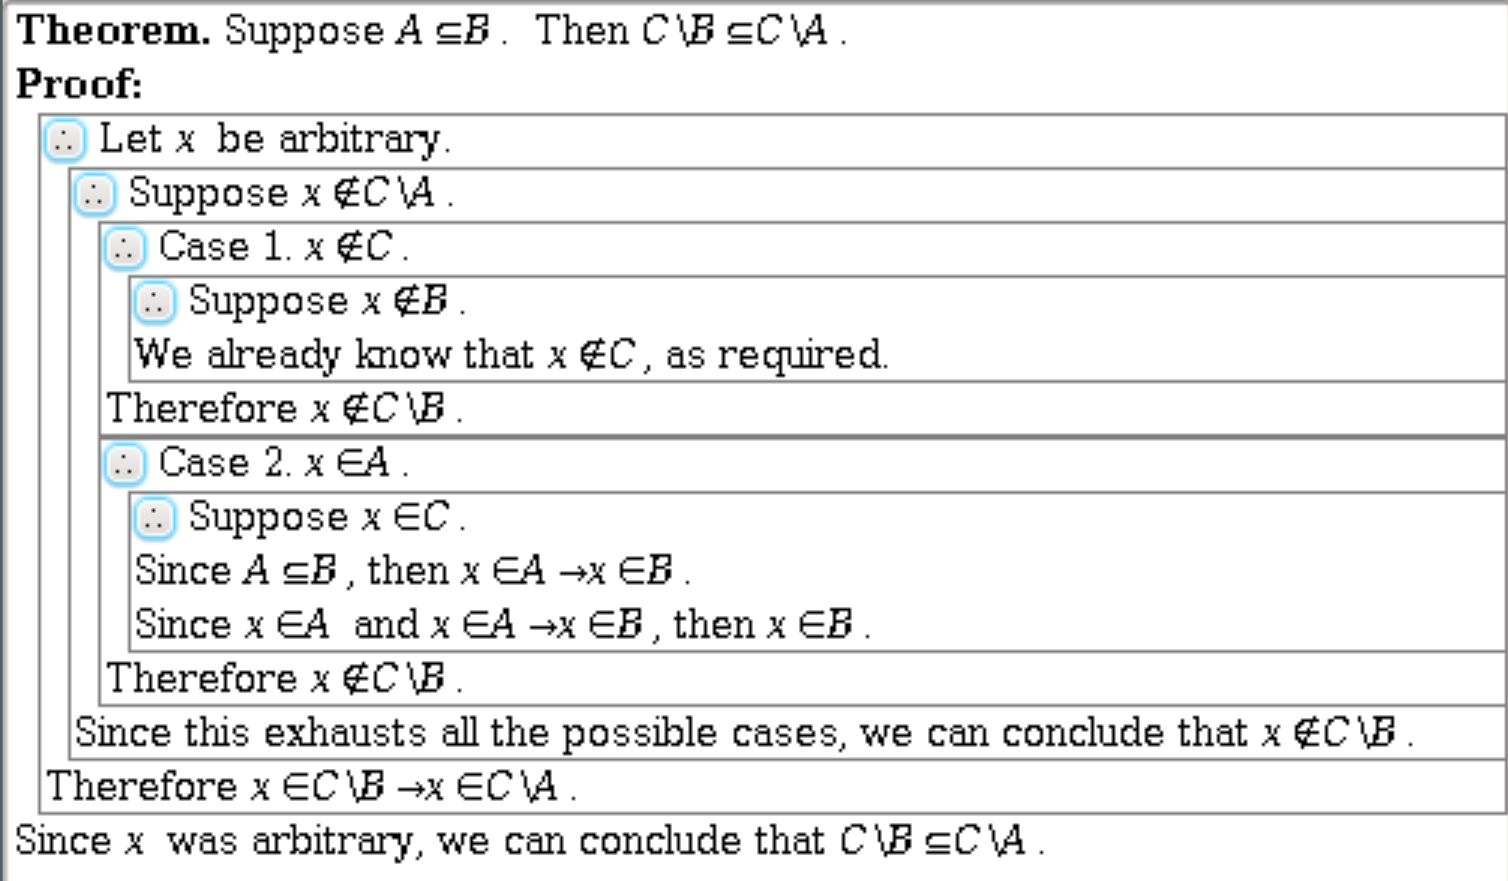
\includegraphics[width=\textwidth]{3_4_3}

\vspace{30pt}

$^{\textit{P}}_{\, \textit{D}}$ *4. Prove that if $A \subseteq B$ and $A \nsubseteq C$ then $B \nsubseteq C$.
\vspace{30pt}

\textbf{3.4.4.pd}
\vspace{10pt}

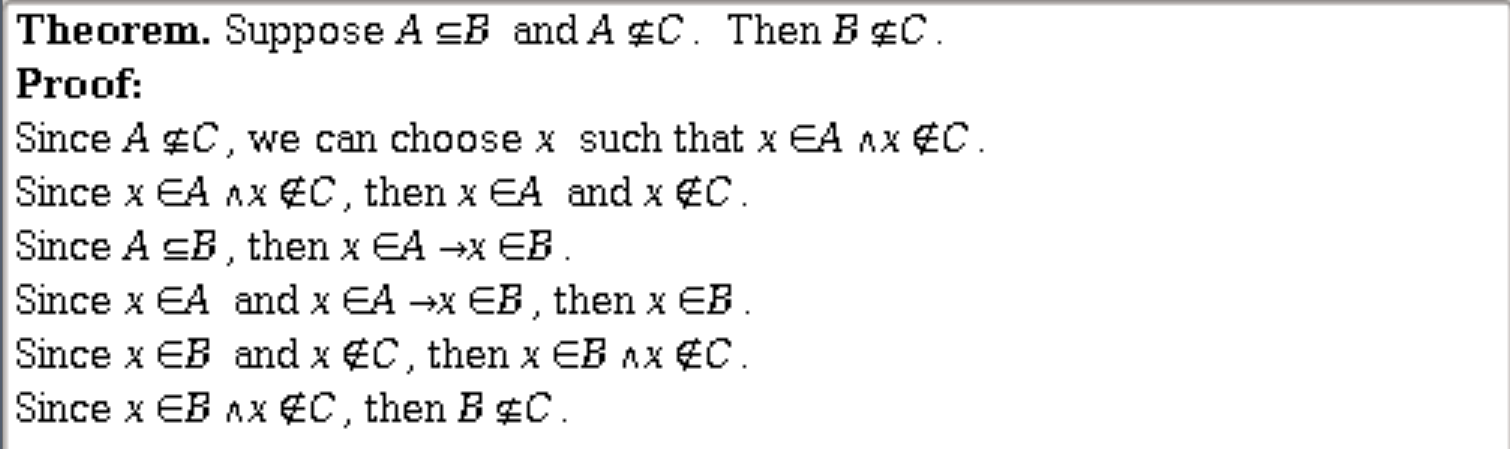
\includegraphics[width=\textwidth]{3_4_4}

\vspace{30pt}

$^{\textit{P}}_{\, \textit{D}}$ 5. Prove that if $A \subseteq B \setminus C$ and $A \neq \varnothing$ then $B \nsubseteq C$.
\vspace{30pt}

\textbf{3.4.5.pd}
\vspace{10pt}

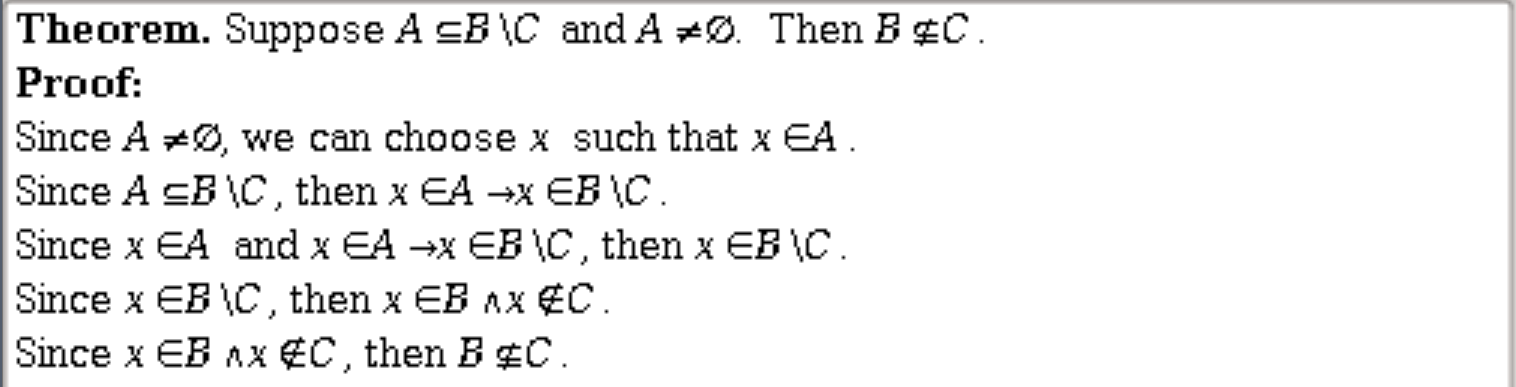
\includegraphics[width=\textwidth]{3_4_5}

\vspace{30pt}

6. Prove that for any sets A, B, and C, $A \setminus (B \cap C) = (A \setminus B) \cup (A \setminus C)$,
by finding a string of equivalences starting with $x \in A \setminus (B \cap C)$ and
ending with $x \in (A \setminus B) \cup (A \setminus C)$. (See Example 3.4.4.)
\vspace{30pt}

\textbf{Theorem.} For any sets A, B, and C, $A \setminus (B \cap C) = (A \setminus B) \cup (A \setminus C)$,

\textit{Proof.} Let x be arbitrary. Then

$x \in A \setminus (B \cap C)$ iff $x \in A \land \neg (x \in B \land x \in C)$

\quad \quad \quad \quad \quad \quad \quad iff $x \in A \land (x \notin B \lor x \notin C)$

\quad \quad \quad \quad \quad \quad \quad iff $(x \in A \land x \notin B) \lor (x \in A \land x \notin C)$

\quad \quad \quad \quad \quad \quad \quad iff $x \in (A \setminus B) \lor x \in (A \setminus C)$

\quad \quad \quad \quad \quad \quad \quad iff $x \in (A \setminus B) \cup (A \setminus C)$

Thus, $\forall x (x \in A \setminus (B \cap C) \leftrightarrow x \in (A \setminus B) \cup (A \setminus C))$, so $A \setminus (B \cap C) = (A \setminus B) \cup (A \setminus C)$.

\vspace{30pt}

$^{\textit{P}}_{\, \textit{D}}$ *7. Use the methods of this chapter to prove that for any sets A and B, $\mathcal{P} (A \cap B) = \mathcal{P} (A) \cap \mathcal{P} (B)$.
\vspace{30pt}

\textbf{3.4.7.pd}
\vspace{10pt}

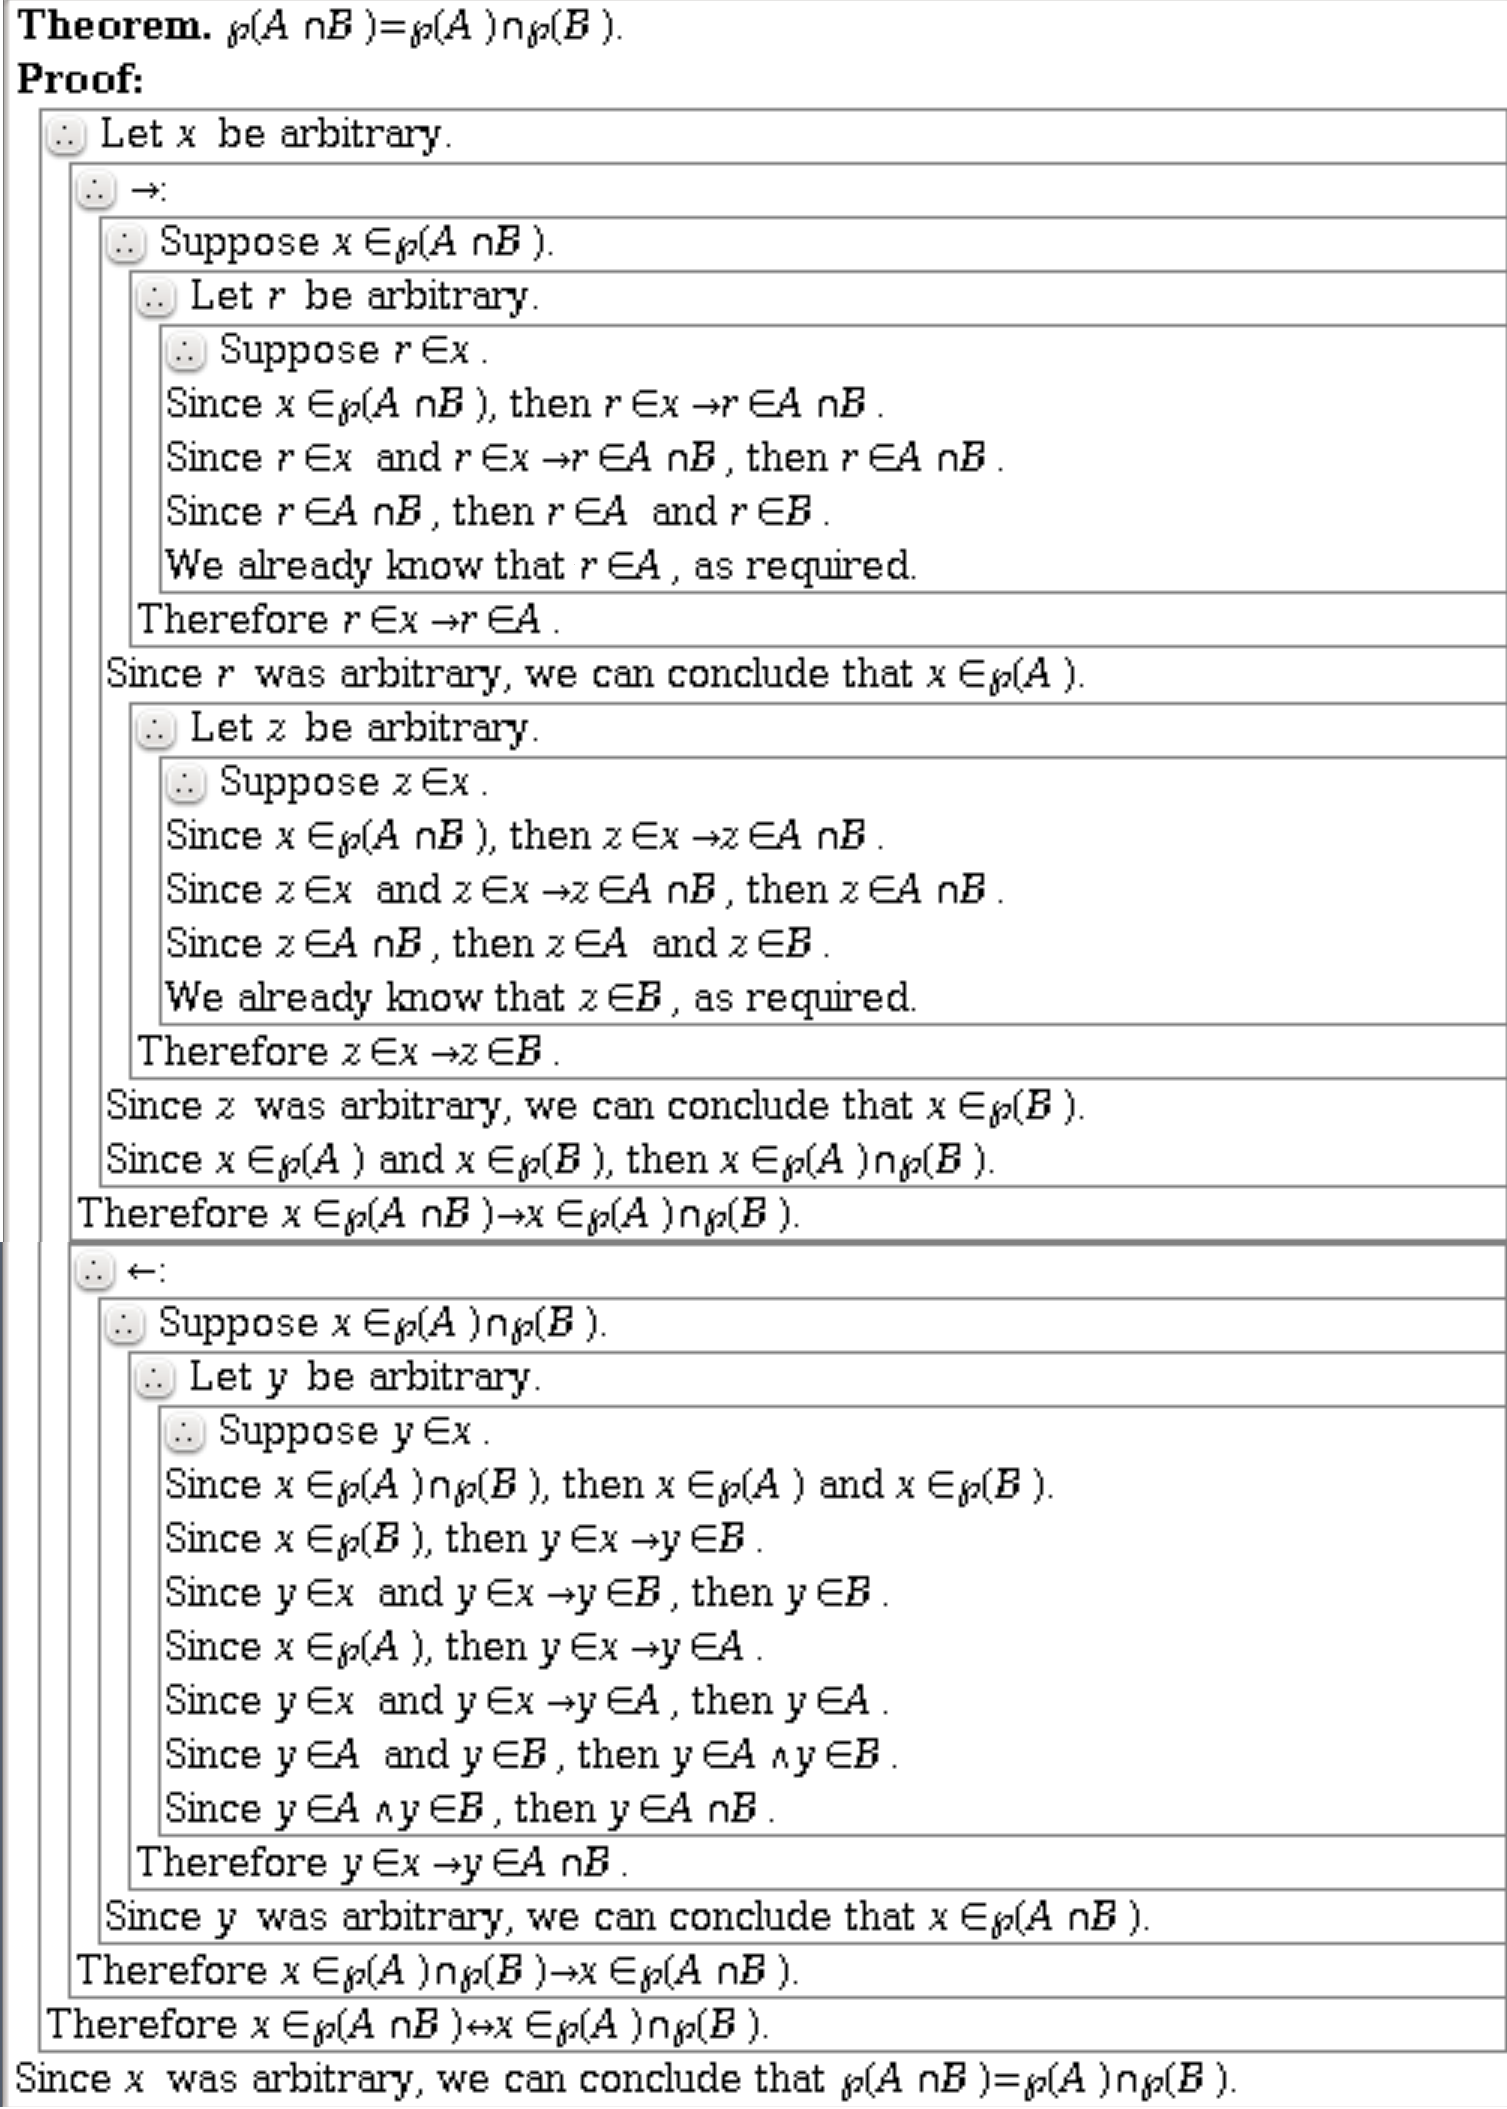
\includegraphics[width=\textwidth]{3_4_7}

\vspace{30pt}

$^{\textit{P}}_{\, \textit{D}}$ 8. Prove that $A \subseteq B$ iff $\mathcal{P} (A) \subseteq \mathcal{P} (B)$.
\vspace{30pt}

\textbf{3.4.8.pd}
\vspace{10pt}

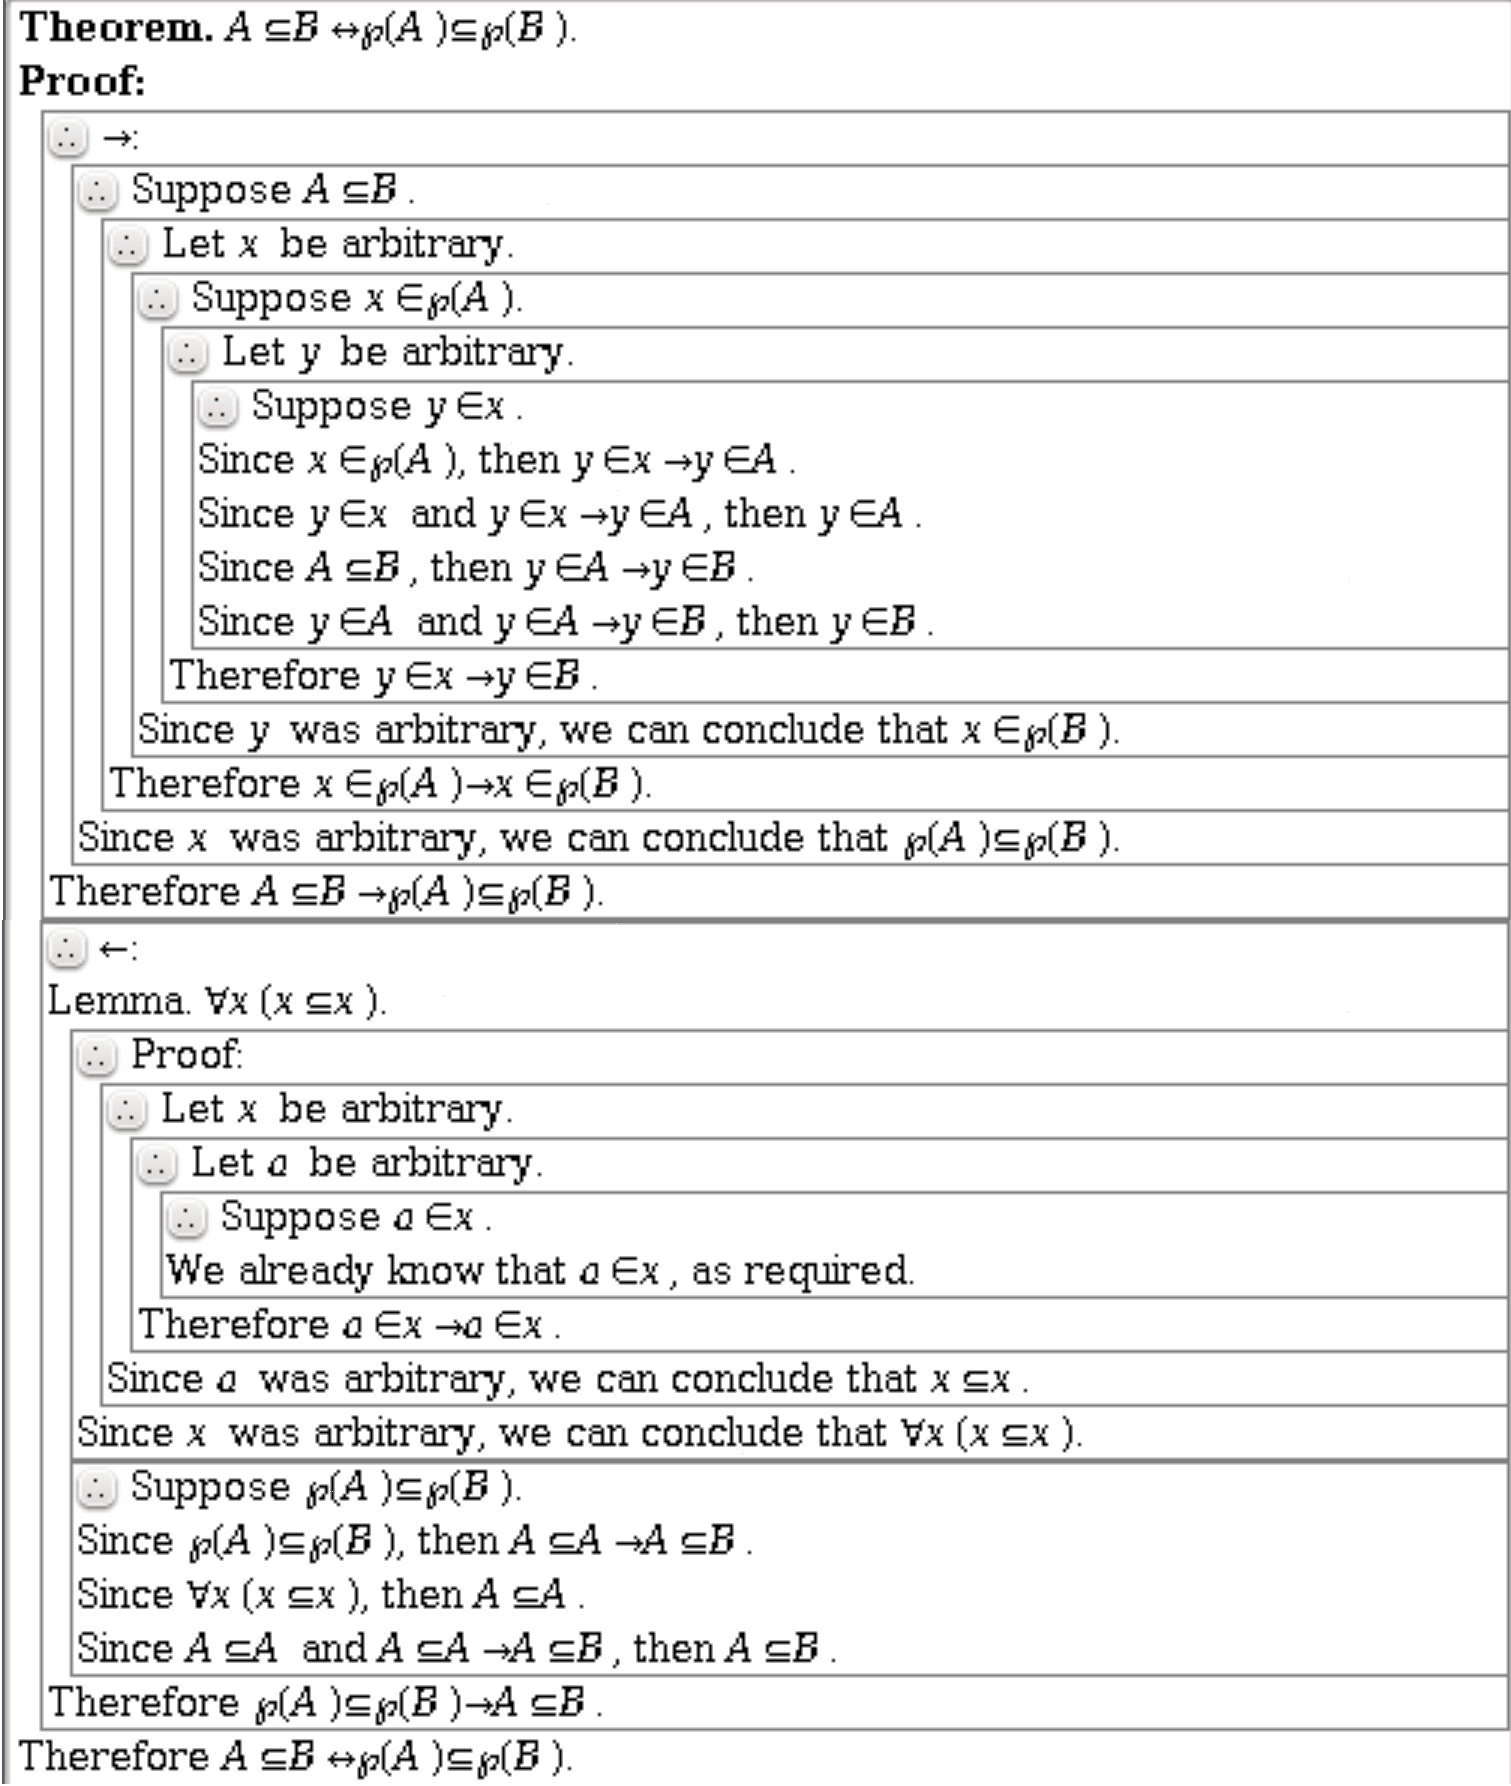
\includegraphics[width=\textwidth]{3_4_8}

\vspace{30pt}

*9. Prove that if x and y are odd integers, then $x y$ is odd.
\vspace{30pt}

$\exists k \in \mathbb{Z} (x = 2k + 1)$

$\exists m \in \mathbb{Z} (y = 2m + 1)$

$x = 2k + 1$

$y = 2m + 1$

$xy$

$(2k + 1)(2m + 1)$

$4km + 2k + 2m + 1$

$2(2km + k + m) + 1$

\centerline{
  \begin{tabular}{l l}
  \textit{Givens} & \textit{Goal} \\
  $\exists k \in \mathbb{Z} (x = 2k + 1)$ & $\exists n \in \mathbb{Z} (xy = 2n + 1)$ \\
  $\exists m \in \mathbb{Z} (y = 2m + 1)$ &           \\
  \end{tabular}}
\vspace{10pt}

\centerline{
  \begin{tabular}{l l}
  \textit{Givens} & \textit{Goal} \\
    $k \in \mathbb{Z}$ & $\exists n \in \mathbb{Z} (xy = 2n + 1)$ \\
    $x = 2k + 1$ & \\
    $m \in \mathbb{Z}$ & \\
    $y = 2m + 1$ & \\
  \end{tabular}}
\vspace{10pt}

Let $n = 2km + k + m$

$(2k+1)(2m+1) = 2n + 1$

$4km + 2k + 2m + 1 = 4km + 2k + 2m + 1$
\vspace{20pt}

\textbf{Theorem.} If x and y are odd integers, then $x y$ is odd.

\textit{Proof.}
Suppose $x$ and $y$ are odd. Let $x = 2k + 1$ for some integer $k$ and $y = 2m + 1$ for some integer $y$.
Therefore, $(2k+1)(2m+1) = 2(2km + k + m) + 1$, so since $2km + k + m$ is an integer, $x y$ is odd.

\vspace{30pt}

10. Prove that for every integer n, $n^3$ is even iff n is even.
\vspace{30pt}

\centerline{
  \begin{tabular}{l l}
  \textit{Givens} & \textit{Goal} \\
    $n \in \mathbb{Z}$ & $n^3 \text{ is even}$ \\
    $n \text{ is even}$ & \\
  \end{tabular}}
\vspace{10pt}

\centerline{
  \begin{tabular}{l l}
  \textit{Givens} & \textit{Goal} \\
    $n \in \mathbb{Z}$ & $\exists k \in \mathbb{Z}(n^3 = 2k)$ \\
    $\exists k \in \mathbb{Z}(n = 2k)$ & \\
  \end{tabular}}
\vspace{10pt}

\centerline{
  \begin{tabular}{l l}
  \textit{Givens} & \textit{Goal} \\
    $n \in \mathbb{Z}$ & $\exists k \in \mathbb{Z}(n^3 = 2k)$ \\
    $k \in \mathbb{Z}$ & \\
    $n = 2k$ & \\
 \end{tabular}}
\vspace{10pt}

$(2k)^3 = 8k^3 = 2(4k^3)$

\centerline{
  \begin{tabular}{l l}
  \textit{Givens} & \textit{Goal} \\
    $n \in \mathbb{Z}$ & $n^3 \text{ is odd}$ \\
    $n \text{ is odd}$ & \\
 \end{tabular}}
\vspace{10pt}

\centerline{
  \begin{tabular}{l l}
  \textit{Givens} & \textit{Goal} \\
    $n \in \mathbb{Z}$ & $\exists k \in \mathbb{Z}(n^3 = 2k + 1)$ \\
    $\exists k \in \mathbb{Z}(n = 2k + 1)$ & \\
 \end{tabular}}
\vspace{10pt}

\centerline{
  \begin{tabular}{l l}
  \textit{Givens} & \textit{Goal} \\
    $n \in \mathbb{Z}$ & $\exists j \in \mathbb{Z}(n^3 = 2j + 1)$ \\
    $k \in \mathbb{Z}$ & \\
    $n = 2k + 1$ & \\
 \end{tabular}}
\vspace{10pt}

$(2k+1)^3 = 8k^3+3(4k^2*1)+3(2k*1)+1 = 8k^3+12k^2+6k+1 = 2(4k^3+6k^2+3)+1$, so
$j = 4k^3+6k^2+3$
\vspace{20pt}

\textbf{Theorem.} For every integer n, $n^3$ is even iff n is even.

\textit{Proof.} ($\leftarrow$) Suppose n is even. Then for some integer k, $n = 2k$. Therefore,
$n^3 = 8k^3 = 2(4k^3)$, so since $4k^3$ is an integer, $n^3$ is even. Thus, if $n$ is even then $n^3$ is even.

($\rightarrow$) Suppose n is odd. Then $n = 2k + 1$ for some integer k. Therefore,
$n^3 = (2k+1)^3 =8k^3+12k^2+6k+1 = 2(4k^3+6k^2+3) + 1$, so since $4k^3+6k^2+3$ is an integer, $n^3$ is odd.
Thus, if $n^3$ is even then $n$ is even.

\vspace{30pt}

11. Consider the following putative theorem:

\textbf{Theorem?} Suppose m is an even integer and n is an odd integer. Then
$n^2 - m^2 = n + m$.

\hspace{12pt}(a) What's wrong with the following proof of the theorem?

\textit{Proof.} Since m is even, we can choose some integer k such that
m = 2k. Similarly, since n is odd we have n = 2k + 1. Therefore
$$n^2 - m^2 = (2k + 1)^2 - (2k)^2 = 4k^2 + 4k + 1 - 4k^2 = 4k + 1
= (2k + 1) + (2k) = n + m.$$

\hspace{12pt}(b) Is the theorem correct? Justify your answer with either a proof or a
counterexample.
\vspace{30pt}

(a) We can't choose k to be some integer 2 times. So, this sentence: "Similarly, since n is odd we have n = 2k + 1" should be turned to something like that: "Similarly, since n is odd we have n = 2m + 1".

\vspace{20pt}

(b) $m = 2$

$n = 5$

$5^2 - 2^2 \neq 5 + 2$

$25 - 4 \neq 7$

$19 \neq 7$

\vspace{30pt}

*12. Prove that $\forall x \in \mathbb{R}[\exists y \in \mathbb{R}(x + y = x y) \leftrightarrow x \neq 1]$.
\vspace{30pt}

\centerline{
  \begin{tabular}{l l}
  \textit{Givens} & \textit{Goal} \\
    $$ & $\forall x \in \mathbb{R}[\exists y \in \mathbb{R}(x + y = x y) \leftrightarrow x \neq 1]$ \\
 \end{tabular}}
\vspace{10pt}

Let x be an arbitrary rational number.

\centerline{
  \begin{tabular}{l l}
  \textit{Givens} & \textit{Goal} \\
    $$ & $\exists y \in \mathbb{R}(x + y = x y) \leftrightarrow x \neq 1$ \\
 \end{tabular}}
\vspace{10pt}

\centerline{$(\rightarrow)$}

\centerline{
  \begin{tabular}{l l}
  \textit{Givens} & \textit{Goal} \\
    $\exists y \in \mathbb{R}(x + y = x y)$ & $x \neq 1$ \\
 \end{tabular}}
\vspace{10pt}

\centerline{
  \begin{tabular}{l l}
  \textit{Givens} & \textit{Goal} \\
    $x + y = x y$ & $x \neq 1$ \\
    $y \in \mathbb{R}$ & \\
 \end{tabular}}
\vspace{10pt}

\centerline{
  \begin{tabular}{l l}
  \textit{Givens} & \textit{Goal} \\
    $x + y = x y$ & Contradiction \\
    $y \in \mathbb{R}$ & \\
    $x = 1$
 \end{tabular}}
\vspace{10pt}

\centerline{
  \begin{tabular}{l l}
  \textit{Givens} & \textit{Goal} \\
    $x + y = x y$ & $x + y \neq x y$ \\
    $y \in \mathbb{R}$ & \\
    $x = 1$
 \end{tabular}}
\vspace{10pt}

Contradiction: $1 + y \neq y$
\vspace{20pt}

\centerline{$(\leftarrow)$}

\centerline{
  \begin{tabular}{l l}
  \textit{Givens} & \textit{Goal} \\
    $x \neq 1$ & $\exists y \in \mathbb{R}(x + y = x y)$ \\
 \end{tabular}}
\vspace{10pt}

Let $y = \frac{x}{x-1}$

$x + \frac{x}{x-1} = x \frac{x}{x-1}$

$\frac{x^2 - x + x}{x-1} = \frac{x^2}{x-1}$ 

$\frac{x^2}{x-1} = \frac{x^2}{x-1}$ 
\vspace{20pt}

\textbf{Theorem.} $\forall x \in \mathbb{R}[\exists y \in \mathbb{R}(x + y = x y) \leftrightarrow x \neq 1]$.

\textit{Proof.} Let x be an arbitrary rational number.

($\rightarrow$) Let $x + y = xy$ for some rational number y. Suppose $x = 1$. Since $x = 1$ and $x + y = xy$, it follows that $1 + y \neq y$ which contradicts to $x + y = xy$. So $x \neq 1$.

($\leftarrow$) Suppose $x \neq 1$. Let $y = \frac{x}{x-1}$

$$x + \frac{x}{x-1} = x \frac{x}{x-1}$$

$$\frac{x^2}{x-1} = \frac{x^2}{x-1}$$

Since x was an arbitrary rational number, thus $\forall x \in \mathbb{R}[\exists y \in \mathbb{R}(x + y = x y) \leftrightarrow x \neq 1]$

\vspace{30pt}

13. Prove that $\exists z \in \mathbb{R} \forall x \in \mathbb{R}^+[\exists y \in \mathbb{R}(y - x = y/x) \leftrightarrow x \neq z]$.
\vspace{30pt}

\centerline{
  \begin{tabular}{l l}
  \textit{Givens} & \textit{Goal} \\
     & $\exists z \in \mathbb{R} \forall x \in \mathbb{R}^+[\exists y \in \mathbb{R}(y - x = y/x) \leftrightarrow x \neq z]$ \\
 \end{tabular}}
\vspace{10pt}

Let $z = y$

\centerline{
  \begin{tabular}{l l}
  \textit{Givens} & \textit{Goal} \\
     & $\forall x \in \mathbb{R}^+[\exists y \in \mathbb{R}(y - x = y/x) \leftrightarrow x \neq z]$ \\
 \end{tabular}}
\vspace{10pt}

Let x be an arbitrary positive real number.

\centerline{
  \begin{tabular}{l l}
  \textit{Givens} & \textit{Goal} \\
     & $\exists y \in \mathbb{R}(y - x = y/x) \leftrightarrow x \neq z$ \\
 \end{tabular}}
\vspace{10pt}

($\rightarrow$)

\centerline{
  \begin{tabular}{l l}
  \textit{Givens} & \textit{Goal} \\
     $\exists y \in \mathbb{R}(y - x = y/x)$ & $x \neq z$ \\
 \end{tabular}}
\vspace{10pt}

\centerline{
  \begin{tabular}{l l}
  \textit{Givens} & \textit{Goal} \\
    $y \in \mathbb{R}$ & $x \neq z$ \\
    $y - x = y/x$ & \\
 \end{tabular}}
\vspace{10pt}

\centerline{
  \begin{tabular}{l l}
  \textit{Givens} & \textit{Goal} \\
    $y \in \mathbb{R}$ & Contradiction \\
    $y - x = y/x$ & \\
    $x = z$ & \\
 \end{tabular}}
\vspace{10pt}

\centerline{
  \begin{tabular}{l l}
  \textit{Givens} & \textit{Goal} \\
    $y \in \mathbb{R}$ & $y - x \neq y/x$ \\
    $y - x = y/x$ & \\
    $x = z$ & \\
 \end{tabular}}
\vspace{10pt}

\centerline{
  \begin{tabular}{l l}
  \textit{Givens} & \textit{Goal} \\
    $y \in \mathbb{R}$ & $y - x \neq y/x$ \\
    $y - x = y/x$ & \\
    $x = y$ & \\
 \end{tabular}}
\vspace{10pt}

$y - x \neq y/x$

$y - y \neq y/y$

$0y \neq 1$

$0 \neq 1$ (contradiction) 

($\leftarrow$)

\centerline{
  \begin{tabular}{l l}
  \textit{Givens} & \textit{Goal} \\
     $x \neq z$ & $\exists y \in \mathbb{R}(y - x = y/x)$ \\
 \end{tabular}}
\vspace{10pt}

\centerline{
  \begin{tabular}{l l}
  \textit{Givens} & \textit{Goal} \\
     $x \neq y$ & $\exists y \in \mathbb{R}(y - x = y/x)$ \\
 \end{tabular}}
\vspace{10pt}

Let $y = 4$

$4 - x = 4/x$

$x + 4/x - 4 = 0$

$x^2 - 4x + 4= 0$

$x = 2$
\vspace{30pt}

\textbf{Theorem.} 13. $\exists z \in \mathbb{R} \forall x \in \mathbb{R}^+[\exists y \in \mathbb{R}(y - x = y/x) \leftrightarrow x \neq z]$.

\textit{Proof.} Let z = y.

Let x be an arbitrary positive real numbers.

\quad ($\rightarrow$) Let $y - x = y/x$ for some rational number $y$. Suppose $x = z$. Then $x = y$.

$$y - x \neq y/x$$

$$y - y \neq y/y$$

$$0y \neq 1$$

$$0 \neq 1$$

\quad So, $y - x \neq y/x$ contradicts to $y - x = y/x$, thus $x \neq z$
\vspace{10pt}

\quad ($\leftarrow$) Suppose $x \neq z$. Then $x \neq y$. Let $y = 4$.

$$4 - x = 4/x$$

$$x + 4/x - 4 = 0$$

$$x^2 - 4x + 4 = 0$$

$$x = 2$$

\quad Therefore, $\exists y \in \mathbb{R}(y - x = y/x)$

Since x was arbitrary positive real number, then $\forall x \in \mathbb{R}^+[\exists y \in \mathbb{R}(y - x = y/x) \leftrightarrow x \neq z]$.

Thus, $\exists z \in \mathbb{R} \forall x \in \mathbb{R}^+[\exists y \in \mathbb{R}(y - x = y/x) \leftrightarrow x \neq z]$

\vspace{30pt}

$^{\textit{P}}_{\, \textit{D}}$ 14. Suppose B is a set and $\mathcal{F}$ is a family of sets. Prove that $\cup\{A \setminus B \mid A \in \mathcal{F}\} \subseteq \cup(\mathcal{F} \setminus \mathcal{P} (B))$.
\vspace{30pt}

\textbf{3.4.14.pd}
\vspace{10pt}

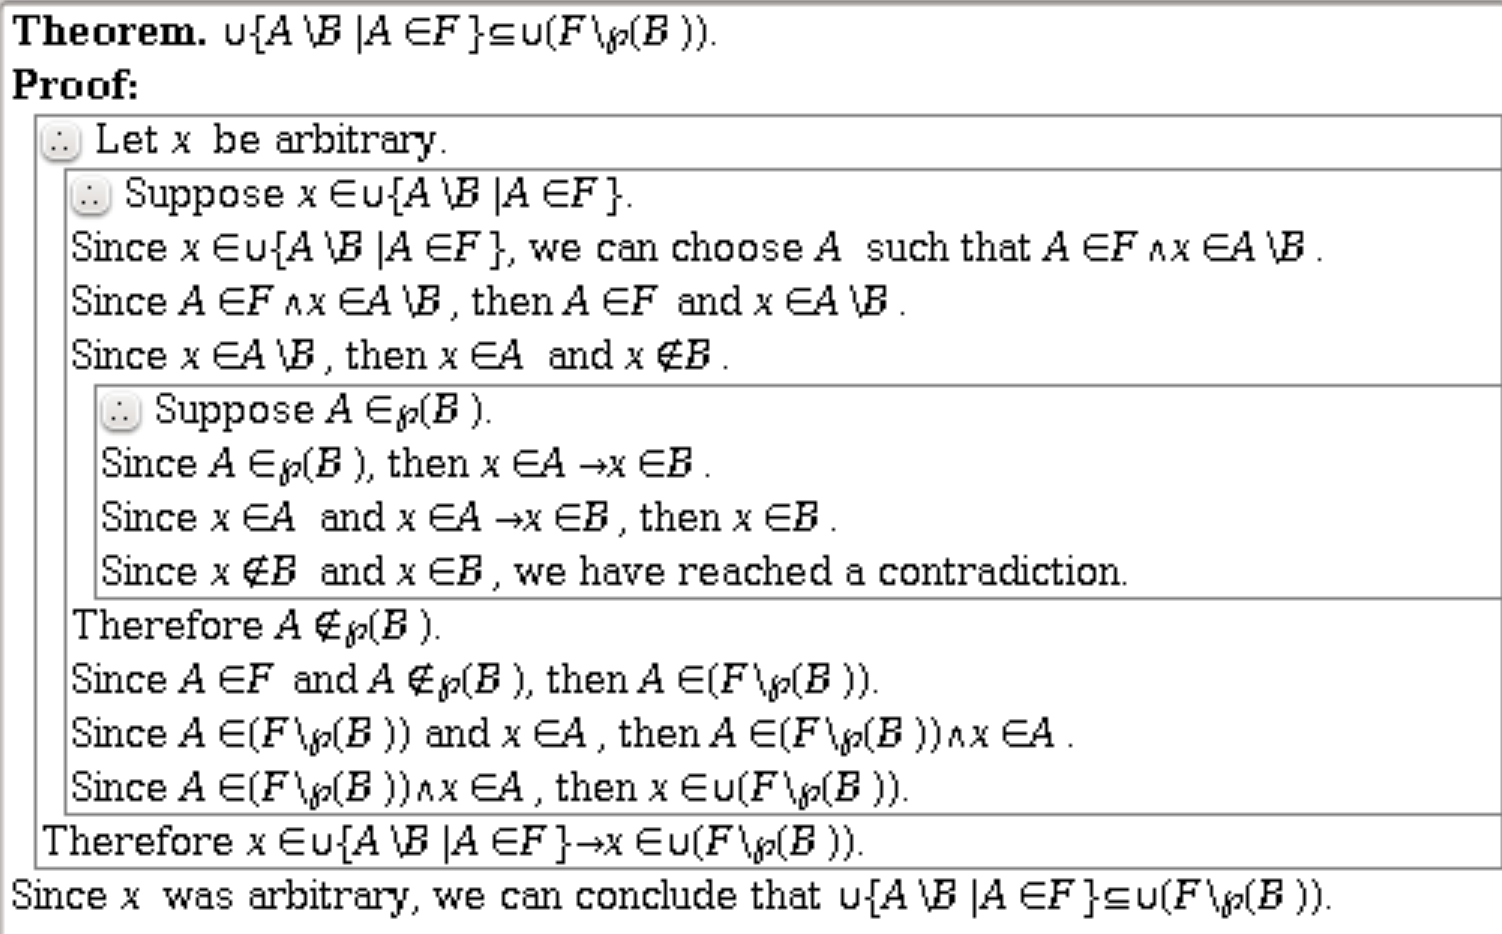
\includegraphics[width=\textwidth]{3_4_14}

\vspace{30pt}

*15. Suppose $\mathcal{F}$ and $\mathcal{G}$ are nonempty families of sets and every element of $\mathcal{F}$
is disjoint from some element of $\mathcal{G}$. Prove that $\cup \mathcal{F}$ and $\cap \mathcal{G}$ are disjoint.
\vspace{30pt}

\centerline{
  \begin{tabular}{l l}
  \textit{Givens} & \textit{Goal} \\
     $\forall x \in \mathcal{F} \exists y \in \mathcal{G}(x \cap y = \varnothing)$ & $\cup \mathcal{F} \cap \cap \mathcal{G} = \varnothing$ \\
 \end{tabular}}
\vspace{10pt}

$\cup \mathcal{F} \cap \cap \mathcal{G} = \varnothing$

$\neg \exists z (z \in \cup \mathcal{F} \land z \in \cap \mathcal{G})$

$\forall z (z \notin \cup \mathcal{F} \lor z \notin \cap \mathcal{G})$

Let z be an arbitrary.

\centerline{
  \begin{tabular}{l l}
  \textit{Givens} & \textit{Goal} \\
     $\forall x \in \mathcal{F} \exists y \in \mathcal{G}(x \cap y = \varnothing)$ & $z \notin \cup \mathcal{F} \lor z \notin \cap \mathcal{G}$ \\
 \end{tabular}}
\vspace{10pt}

\centerline{
  \begin{tabular}{l l}
  \textit{Givens} & \textit{Goal} \\
     $\forall x \in \mathcal{F} \exists y \in \mathcal{G}(x \cap y = \varnothing)$ & $z \in \cup \mathcal{F} \to z \notin \cap \mathcal{G}$ \\
 \end{tabular}}
\vspace{10pt}

\centerline{
  \begin{tabular}{l l}
  \textit{Givens} & \textit{Goal} \\
    $\forall x \in \mathcal{F} \exists y \in \mathcal{G}(x \cap y = \varnothing)$ & $z \notin \cap \mathcal{G}$ \\
    $z \in \cup \mathcal{F}$
 \end{tabular}}
\vspace{10pt}

$z \in \cup \mathcal{F}$

$\exists A (A \in \mathcal{F} \land z \in A)$

\centerline{
  \begin{tabular}{l l}
  \textit{Givens} & \textit{Goal} \\
    $\forall x \in \mathcal{F} \exists y \in \mathcal{G}(x \cap y = \varnothing)$ & $z \notin \cap \mathcal{G}$ \\
    $A_0 \in \mathcal{F}$ & \\
    $z \in A_0$ & \\
 \end{tabular}}
\vspace{10pt}

\centerline{
  \begin{tabular}{l l}
  \textit{Givens} & \textit{Goal} \\
    $\exists y \in \mathcal{G}(A_0 \cap y = \varnothing)$ & $z \notin \cap \mathcal{G}$ \\
    $z \in A_0$ & \\
 \end{tabular}}
\vspace{10pt}

\centerline{
  \begin{tabular}{l l}
  \textit{Givens} & \textit{Goal} \\
    $y \in \mathcal{G}$ & $z \notin \cap \mathcal{G}$ \\
    $z \in A_0$ & \\
    $A_0 \cap y = \varnothing$ & \\
 \end{tabular}}
\vspace{10pt}

$z \notin \cap \mathcal{G}$

$\neg \forall B (B \in \mathcal{G} \to z \in B)$

$\exists B (B \in \mathcal{G} \land z \notin B)$

\centerline{
  \begin{tabular}{l l}
  \textit{Givens} & \textit{Goal} \\
    $y \in \mathcal{G}$ & $\exists B (B \in \mathcal{G} \land z \notin B)$ \\
    $z \in A_0$ & \\
    $A_0 \cap y = \varnothing$ & \\
 \end{tabular}}
\vspace{10pt}

$A_0 \cap y = \varnothing$

$\neg \exists m (m \in A_0 \land m \in y)$

$\forall m (m \in A_0 \to m \notin y)$


\centerline{
  \begin{tabular}{l l}
  \textit{Givens} & \textit{Goal} \\
    $y \in \mathcal{G}$ & $\exists B (B \in \mathcal{G} \land z \notin B)$ \\
    $z \in A_0$ & \\
    $\forall m (m \in A_0 \to m \notin y)$ & \\
 \end{tabular}}
\vspace{10pt}

\centerline{
  \begin{tabular}{l l}
  \textit{Givens} & \textit{Goal} \\
    $y \in \mathcal{G}$ & $\exists B (B \in \mathcal{G} \land z \notin B)$ \\
    $z \notin y$ & \\
 \end{tabular}}
\vspace{10pt}

Let B = y

\centerline{
  \begin{tabular}{l l}
  \textit{Givens} & \textit{Goal} \\
    $y \in \mathcal{G}$ & $y \in \mathcal{G} \land z \notin y$ \\
    $z \notin y$ & \\
 \end{tabular}}
\vspace{10pt}

Proved.

\textbf{Theorem.} If $\mathcal{F}$ and $\mathcal{G}$ are nonempty families of sets and every element of $\mathcal{F}$ is disjoint from some element of $\mathcal{G}$ then $\cup \mathcal{F}$ and $\cap \mathcal{G}$ are disjoint.

\textit{Proof.} Suppose $x \cap y = \varnothing$ for every $x \in \mathcal{F}$ and for some $y \in \mathcal{G}$.

\quad $\cup \mathcal{F} \cap \cap \mathcal{G} = \varnothing$ is equivalent to $\forall z (z \notin \cup \mathcal{F} \lor z \notin \cap \mathcal{G})$.

\quad Let z be an arbitrary element.

\quad \quad Suppose $z \in \cup \mathcal{F}$.

\quad \quad \quad $z \notin \cap \mathcal{G}$ is equivalent to $\exists B (B \in \mathcal{G} \land z \notin B)$.

\quad \quad \quad Let $B = y$

\quad \quad \quad \quad Since $z \in \cup \mathcal{F}$ let choose some $A_0$

\quad \quad \quad \quad such that $A_0 \in \mathcal{F}$ and $z \in A_0$

\quad \quad \quad \quad Since $A_0  \in \mathcal{F}$ and $\forall x \in \mathcal{F} \exists y \in \mathcal{G}(x \cap y = \varnothing)$, it follows that $\exists y \in \mathcal{G}(A_0 \cap y = \varnothing)$.

\quad \quad \quad \quad Since $\exists y \in \mathcal{G}(A_0 \cap y = \varnothing)$ let $y \in \mathcal{G}$ and $A_0 \cap y = \varnothing$.

\quad \quad \quad \quad Since $A_0 \cap y = \varnothing$ and $z \in A_0$, it follows that $z \notin y$

\quad \quad \quad Thus, $y \in \mathcal{G} \land z \notin y$.

\quad \quad Thus, $z \notin \cap \mathcal{G}$ 

\quad Thus, $\forall z (z \notin \cup \mathcal{F} \lor z \notin \cap \mathcal{G})$.

Then $\cup \mathcal{F} \cap \cap \mathcal{G} = \varnothing$.

\vspace{30pt}

$^{\textit{P}}_{\, \textit{D}}$ 16. Prove that for any set A, $A = \cup \mathcal{P} (A)$.
\vspace{30pt}

\textbf{3.4.16.pd}
\vspace{10pt}

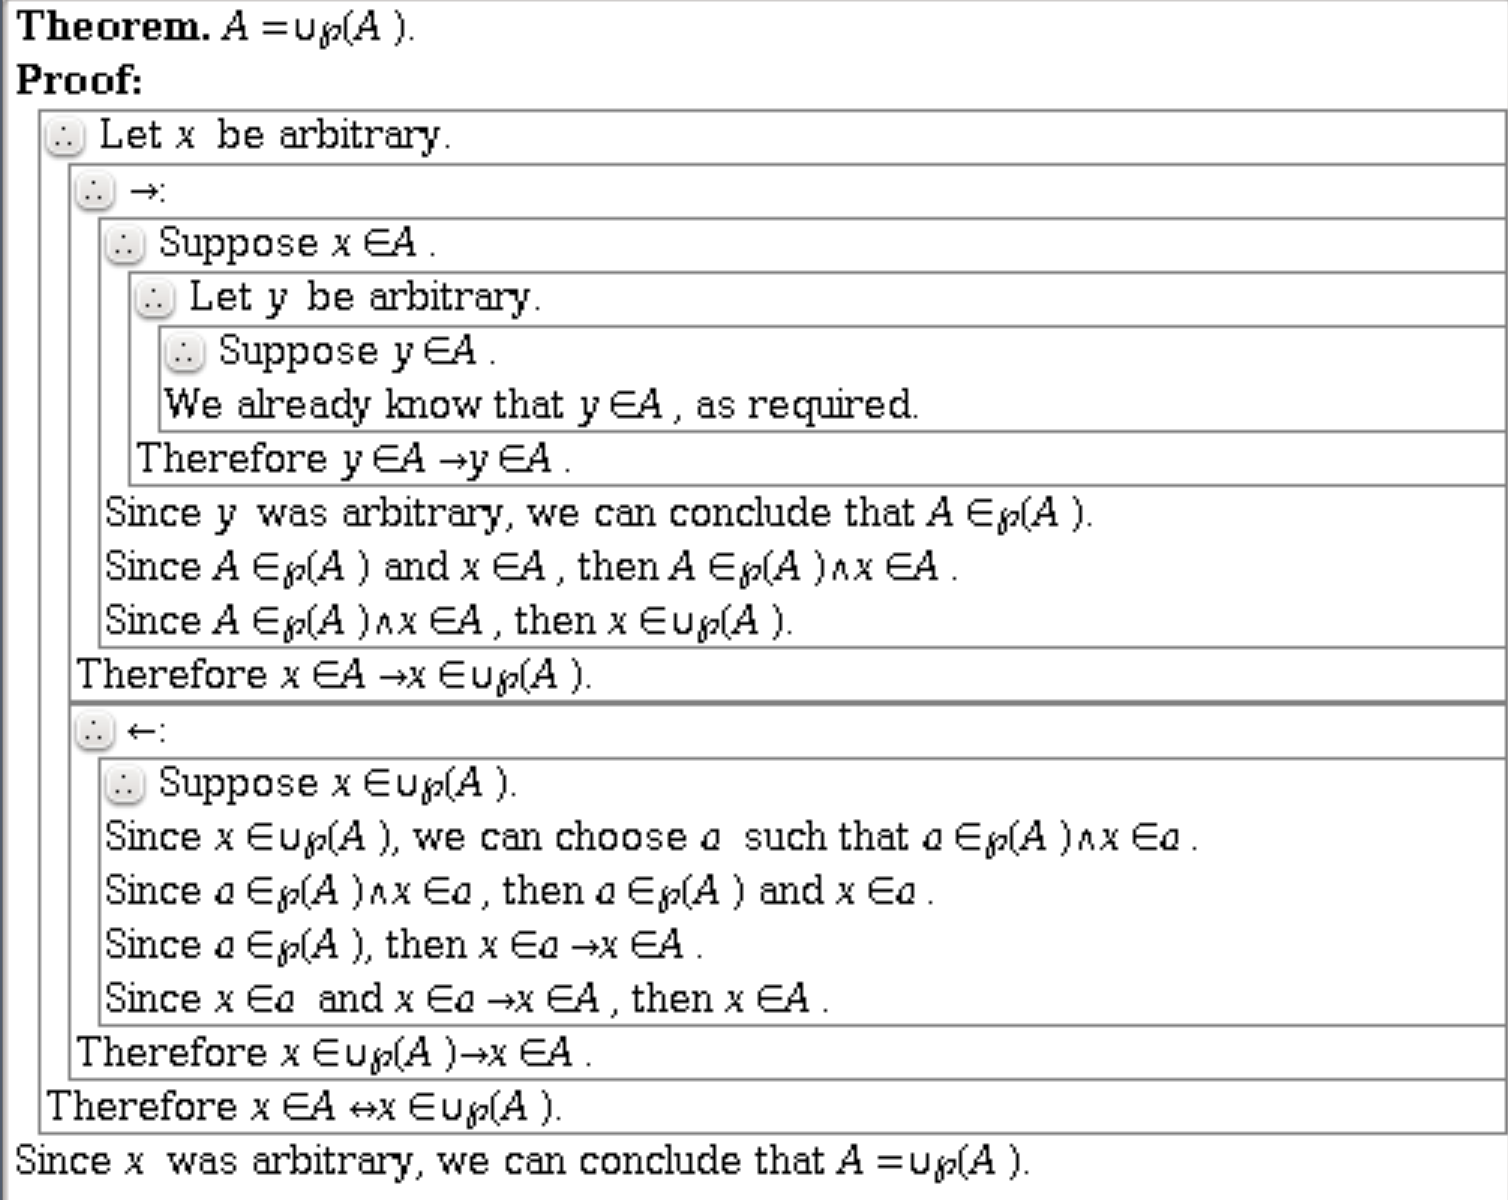
\includegraphics[width=\textwidth]{3_4_16}

\vspace{30pt}

$^{\textit{P}}_{\, \textit{D}}$ *17. Suppose $\mathcal{F}$ and $\mathcal{G}$ are families of sets.


\hspace{12pt}(a) Prove that $\cup (\mathcal{F} \cap \mathcal{G}) \subseteq (\cup\mathcal{F}) \cap (\cup\mathcal{G})$.

\hspace{12pt}(b) What's wrong with the following proof that $(\cup \mathcal{F}) \cap (\cup \mathcal{G}) \subseteq
\cup(\mathcal{F} \cap \mathcal{G})$?

\textit{Proof.} Suppose $x \in (\cup\mathcal{F}) \cap (\cup\mathcal{G})$. This means that $x \in \cup \mathcal{F}$ and $x \in \cup \mathcal{G}$, so $\exists A \in \mathcal{F}(x \in A)$ and $\exists A \in \mathcal{G}(x \in A)$. Thus, we can choose a set A such that $A \in \mathcal{F}$, $A \in \mathcal{G}$, and $x \in A$. Since $A \in \mathcal{F}$ and $A \in \mathcal{G}$, $A \in \mathcal{F} \cap \mathcal{G}$. Therefore $\exists A \in \mathcal{F} \cap \mathcal{G}(x \in A)$, so $x \in \cup(\mathcal{F} \cap \mathcal{G})$. Since x was arbitrary, we can conclude that $(\cup\mathcal{F}) \cap (\cup\mathcal{G}) \subseteq \cup(\mathcal{F} \cap \mathcal{G})$.

\hspace{12pt}(c) Find an example of families of sets $\mathcal{F}$ and $\mathcal{G}$ for which $\cup (\mathcal{F} \cap \mathcal{G}) \neq (\cup\mathcal{F}) \cap (\cup\mathcal{G})$.
\vspace{30pt}

(a)

\textbf{3.4.17.pd}
\vspace{10pt}

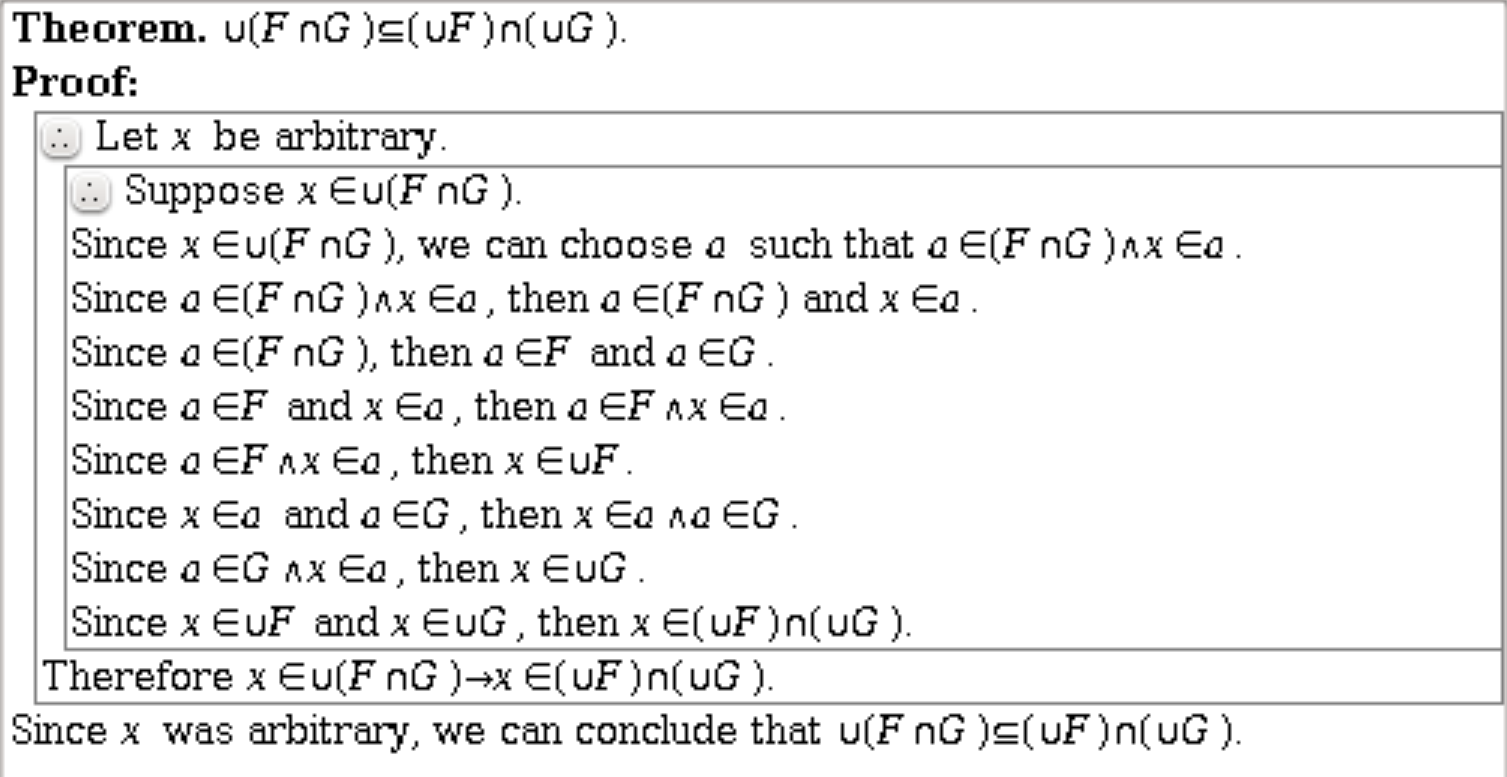
\includegraphics[width=\textwidth]{3_4_17_1}

\vspace{30pt}

(b) "Thus, we can choose a set A such that $A \in \mathcal{F}$, $A \in \mathcal{G}$, and $x \in A$." is wrong conclusion. During existential instantiation you must choose untaken variable.

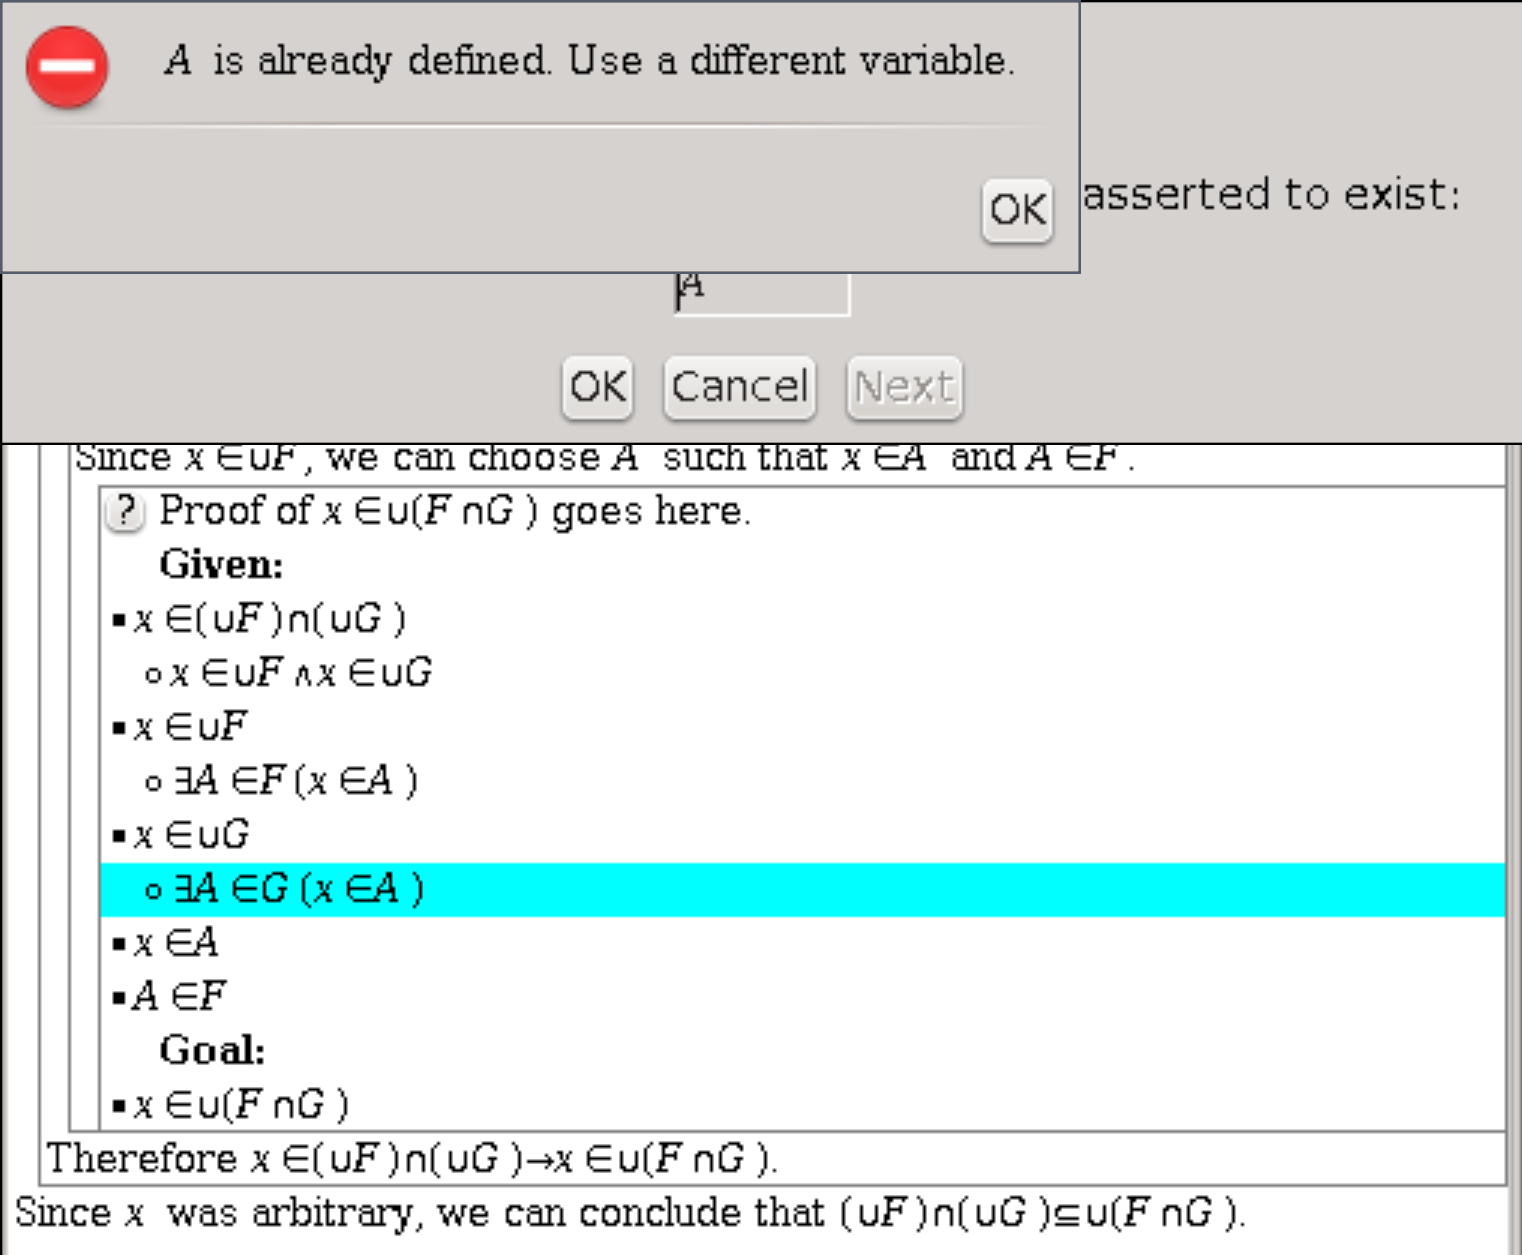
\includegraphics[width=\textwidth]{3_4_17_2}

\vspace{30pt}

(c) $\mathcal{F} = \{\{1\},\{2\}\}$

$\mathcal{G} = \{\{1\},\{1,2\}\}$

$\mathcal{F} \cap \mathcal{G}= \{\{1\}\}$

$\cup (\mathcal{F} \cap \mathcal{G}) = \{1\}$

$\cup \mathcal{F} = \{1, 2\}$

$\cup \mathcal{G} = \{1, 2\}$

$(\cup \mathcal{F}) \cap (\cup \mathcal{G}) = \{1,2\}$

\vspace{30pt}

$^{\textit{P}}_{\, \textit{D}}$ 18. Suppose $\mathcal{F}$ and $\mathcal{G}$ are families of sets. Prove that $(\cup\mathcal{F}) \cap (\cup\mathcal{G}) \subseteq \cup(\mathcal{F} \cap \mathcal{G})$ iff $\forall A \in \mathcal{F} \forall B \in \mathcal{G}(A \cap B \subseteq \cup(\mathcal{F} \cap \mathcal{G}))$.
\vspace{30pt}

\textbf{3.4.18.pd}
\vspace{10pt}

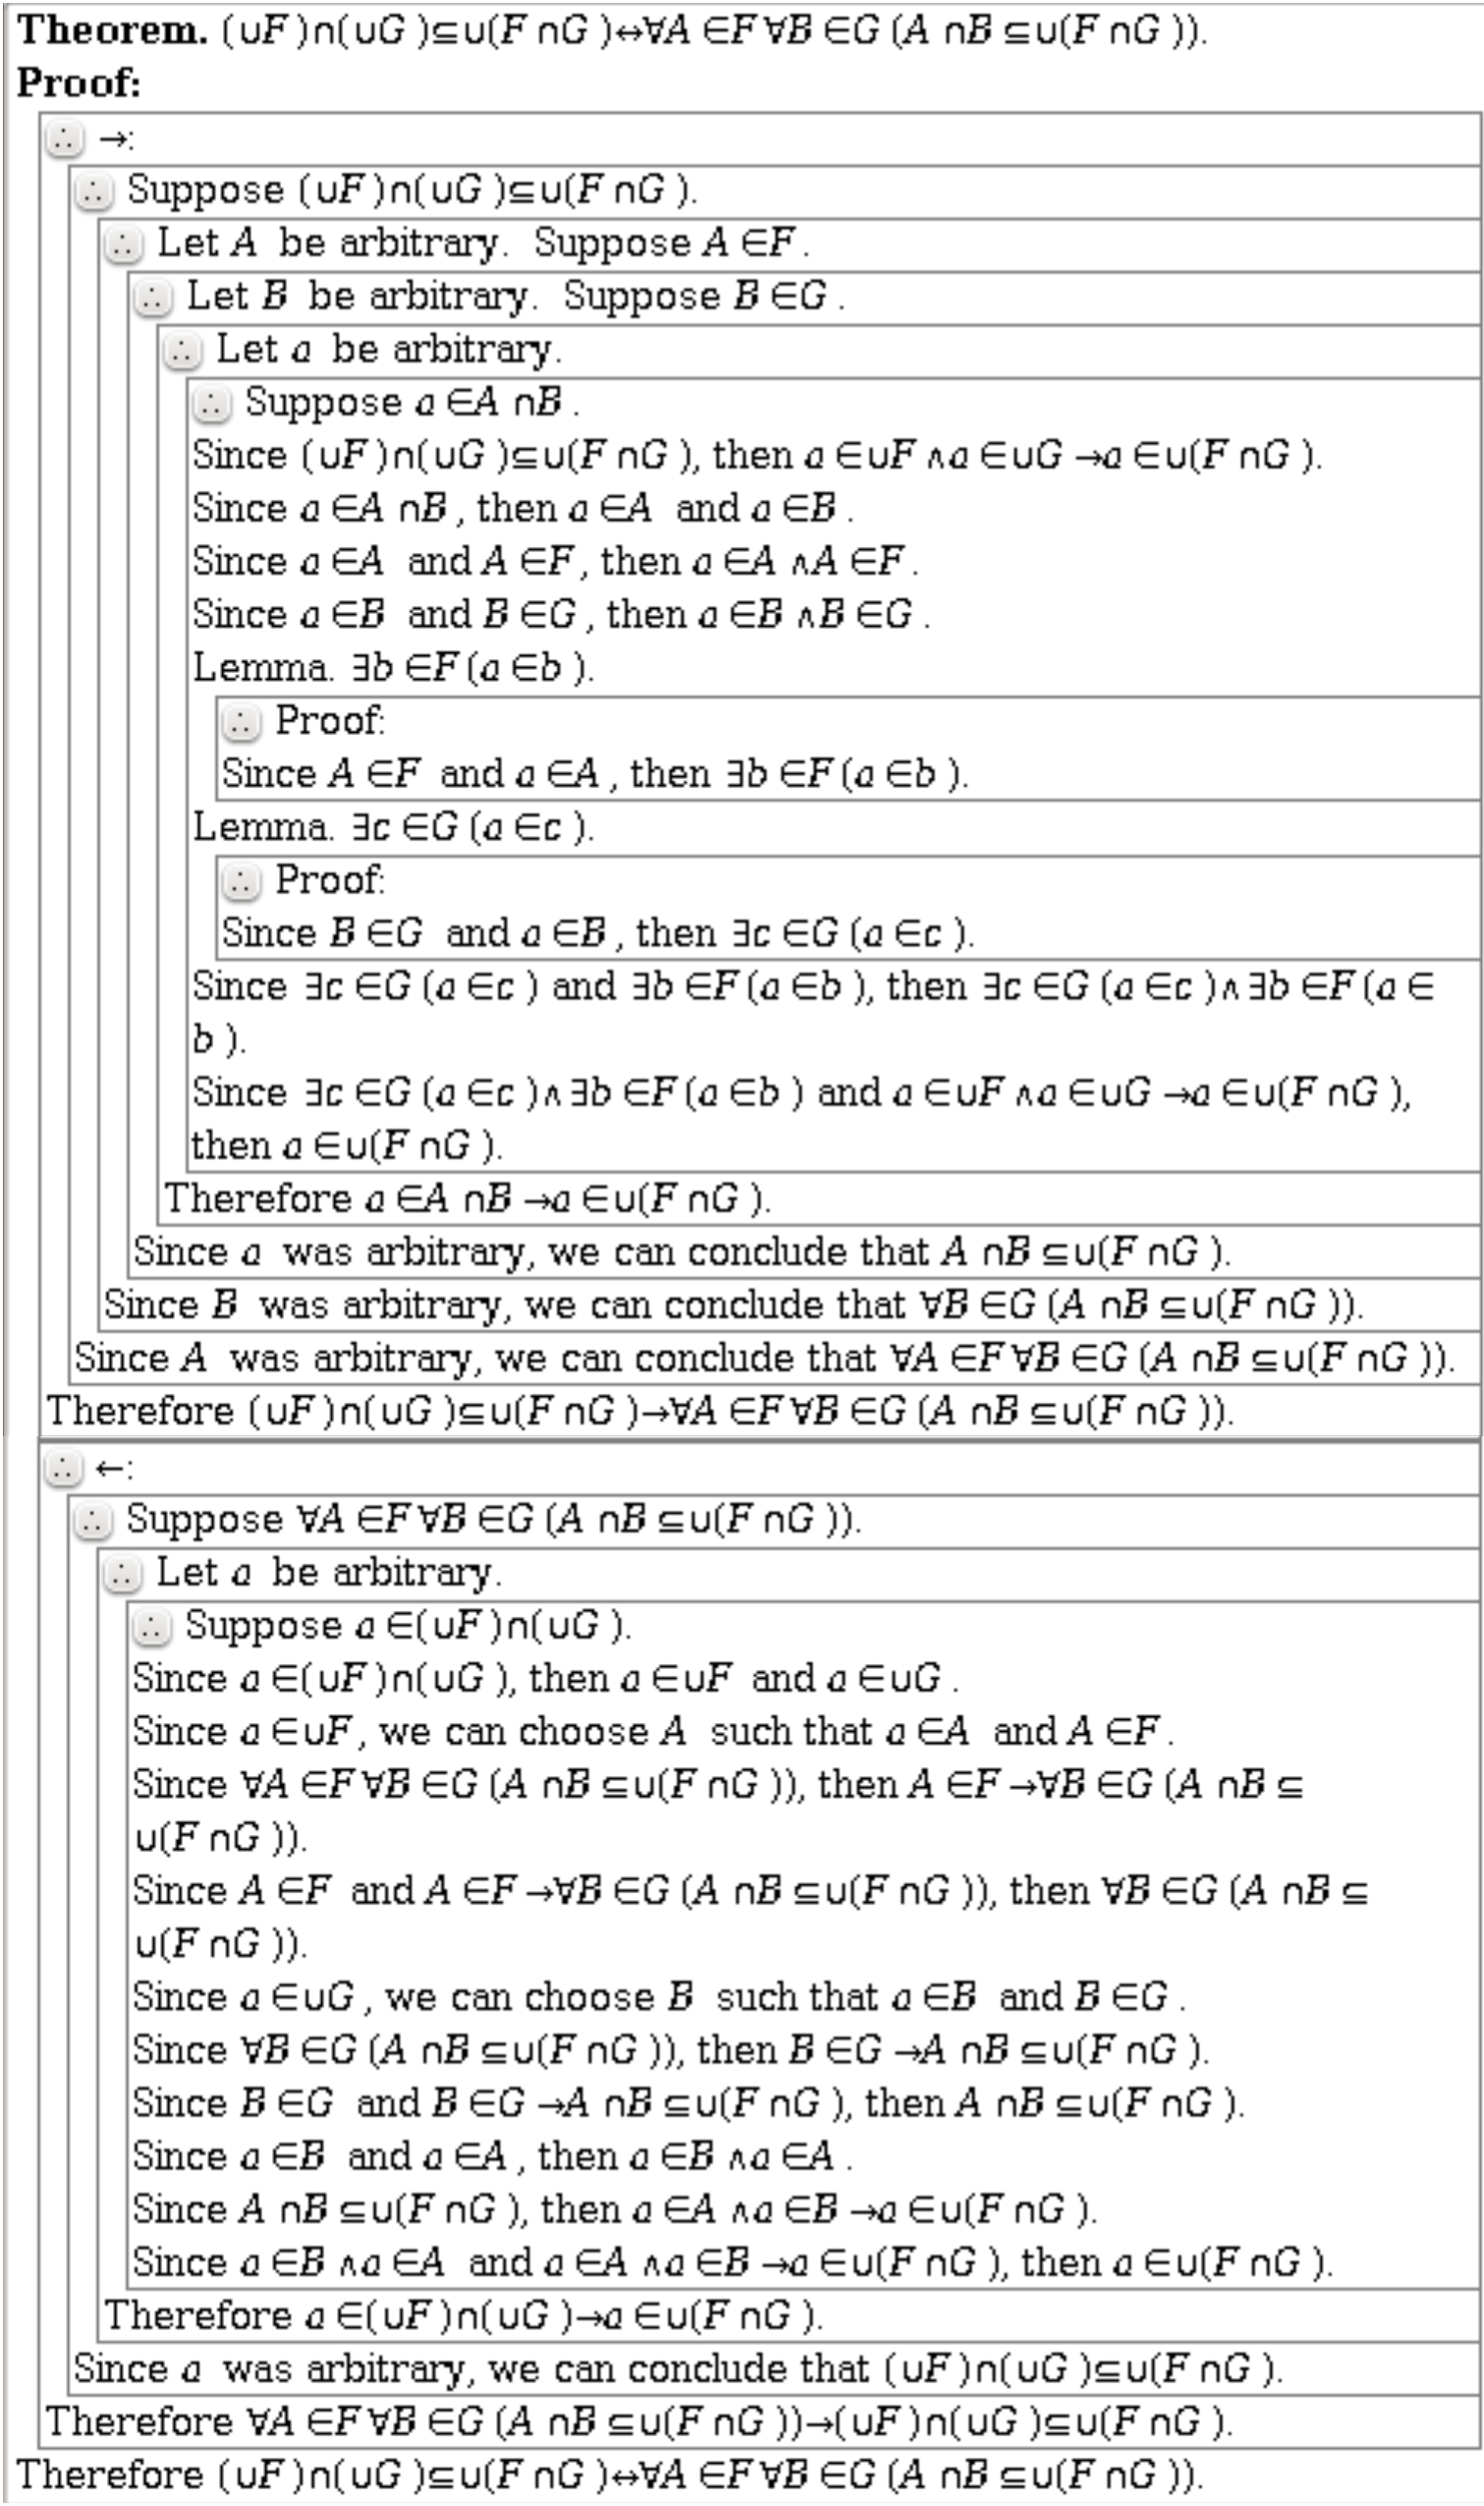
\includegraphics[scale=0.15]{3_4_18}

\vspace{30pt}

$^{\textit{P}}_{\, \textit{D}}$ 19. Suppose $\mathcal{F}$ and $\mathcal{G}$ are families of sets. Prove that $\cup \mathcal{F}$ and $\cup \mathcal{G}$ are disjoint iff for all $A \in \mathcal{F}$ and $B \in \mathcal{G}$, A and B are disjoint.
\vspace{30pt}

\textbf{3.4.19.pd}
\vspace{10pt}

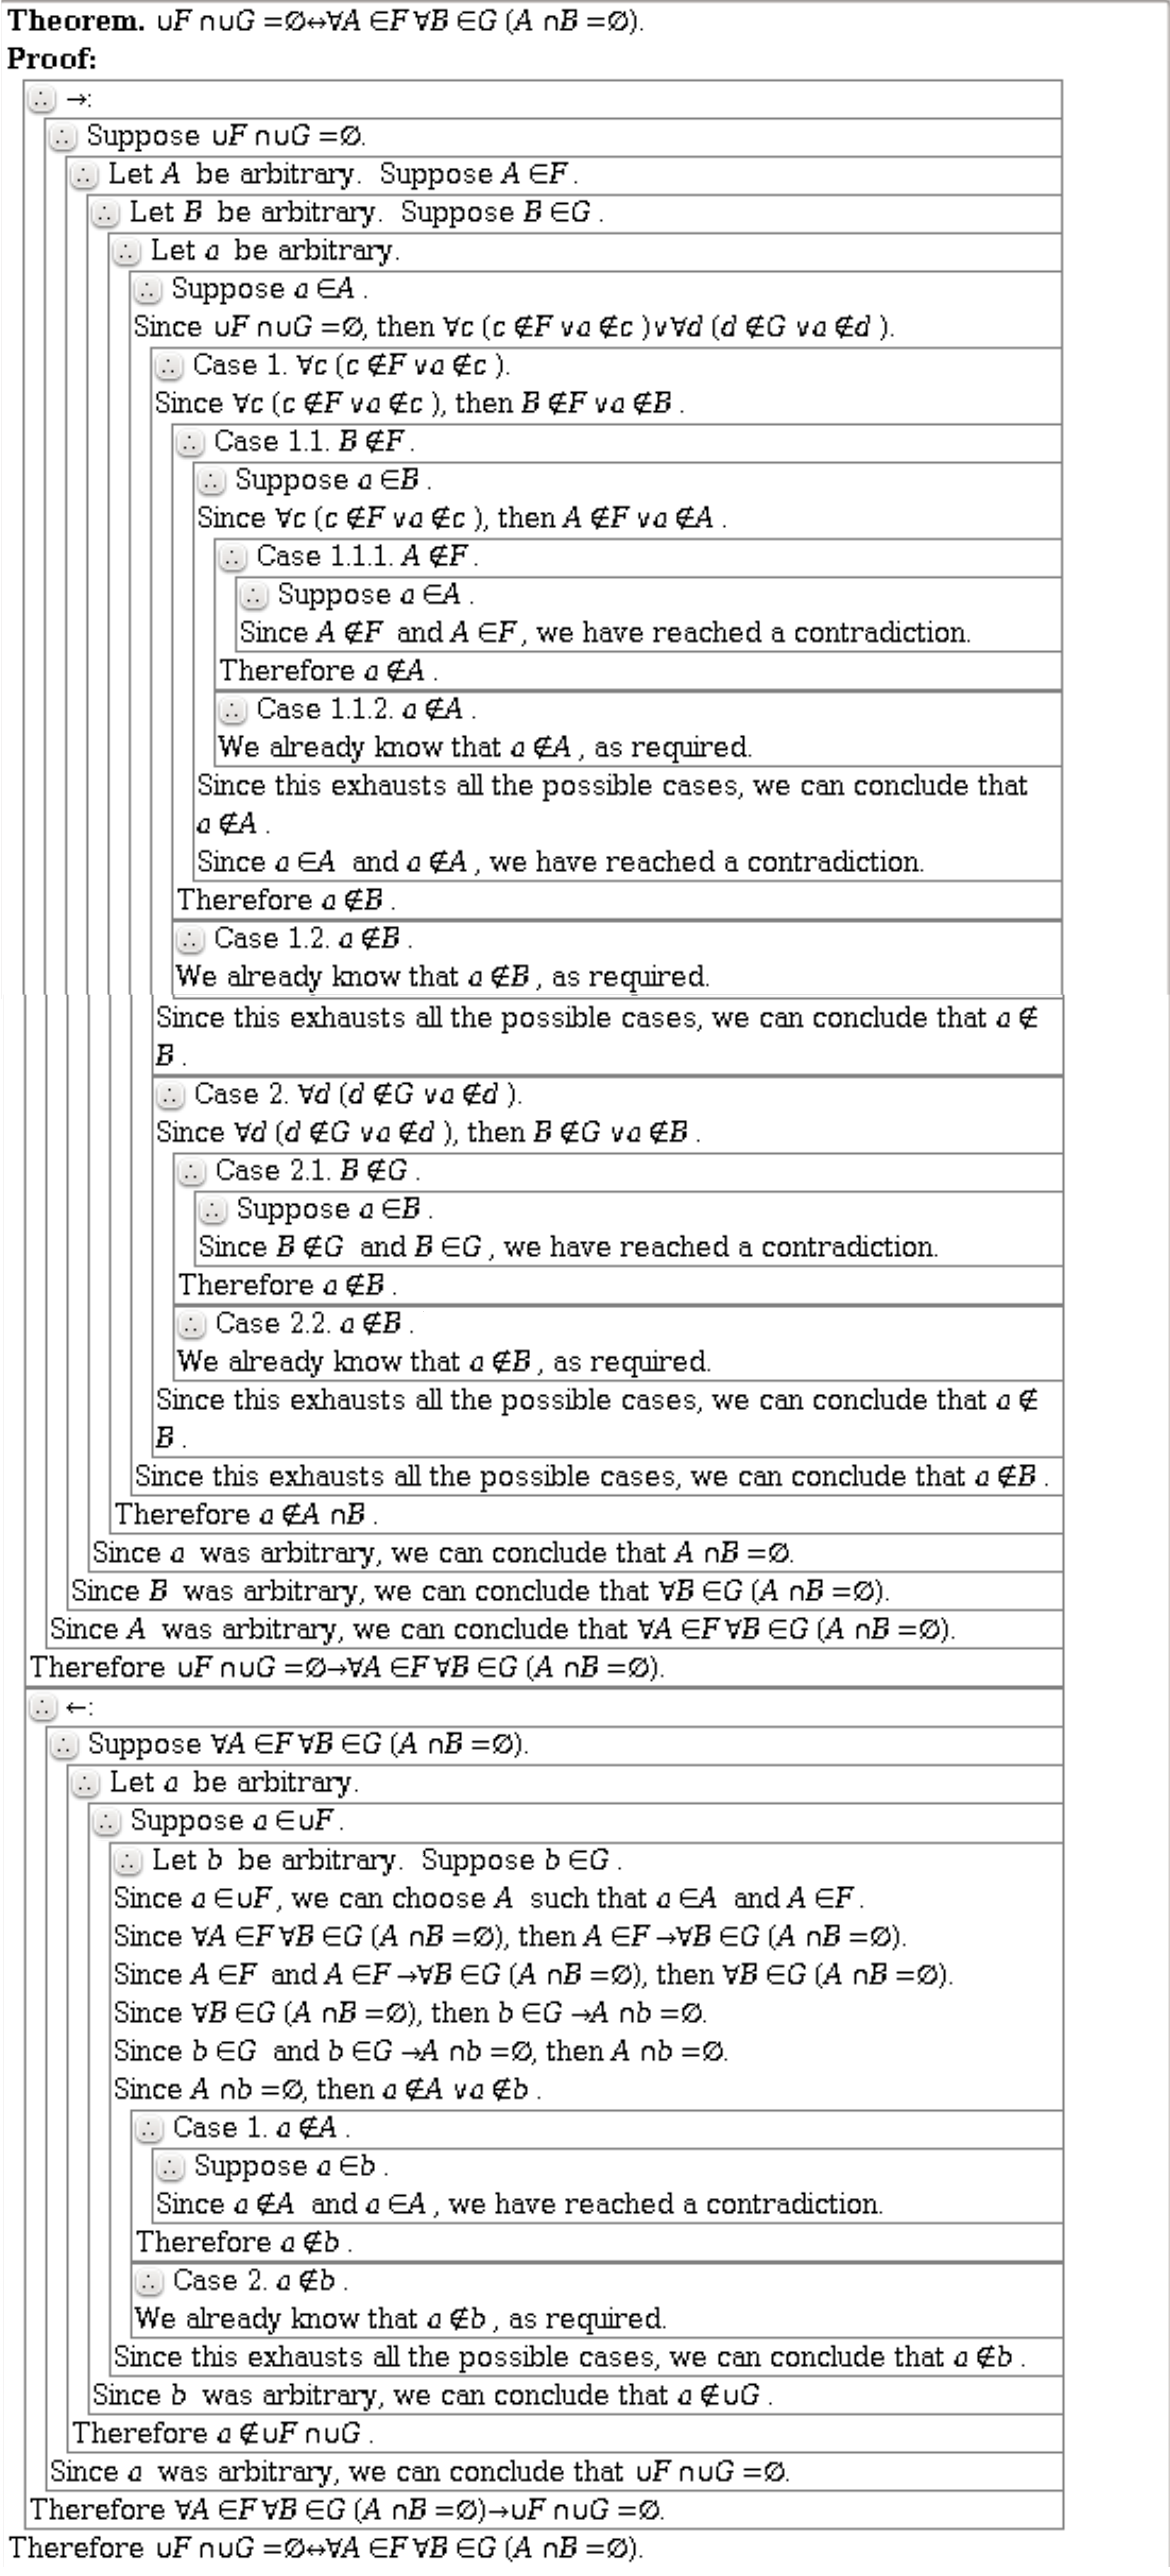
\includegraphics[scale=0.15]{3_4_19}

\vspace{30pt}

$^{\textit{P}}_{\, \textit{D}}$ 20. Suppose $\mathcal{F}$ and $\mathcal{G}$ are families of sets.

\hspace{12pt}(a) Prove that $(\cup\mathcal{F}) \setminus (\cup\mathcal{G}) \subseteq \cup (\mathcal{F} \setminus \mathcal{G})$.

\hspace{12pt}(b) What's wrong with the following proof that $\cup(\mathcal{F} \setminus \mathcal{G}) \subseteq (\cup\mathcal{F}) \setminus (\cup\mathcal{G})$?

\textit{Proof.} Suppose $x \in \cup(\mathcal{F} \setminus \mathcal{G})$. Then we can choose some $A \in \mathcal{F} \setminus \mathcal{G}$ such that $x \in A$. Since $A \in \mathcal{F} \setminus \mathcal{G}$, $A \in \mathcal{F}$ and $A \notin \mathcal{G}$. Since $x \in A$ and $A \in \mathcal{F}$, $x \in \cup \mathcal{F}$. Since $x \in A$ and $A \notin \mathcal{G}$, $x \notin \cup \mathcal{G}$. Therefore $x \in (\cup \mathcal{F}) \setminus (\cup\mathcal{G})$.

\hspace{12pt}(c) Prove that $\cup(\mathcal{F} \setminus \mathcal{G}) \subseteq (\cup\mathcal{F}) \setminus (\cup\mathcal{G})$ iff $\forall A \in (\mathcal{F} \setminus \mathcal{G})\forall B \in \mathcal{G}(A \cap
B = \varnothing)$.

\hspace{12pt}(d) Find an example of families of sets $\mathcal{F}$ and $\mathcal{G}$ for which $\cup (\mathcal{F} \setminus \mathcal{G}) \neq (\cup\mathcal{F}) \setminus (\cup\mathcal{G})$.
\vspace{30pt}

(a)

\textbf{3.4.20.1.pd}
\vspace{10pt}

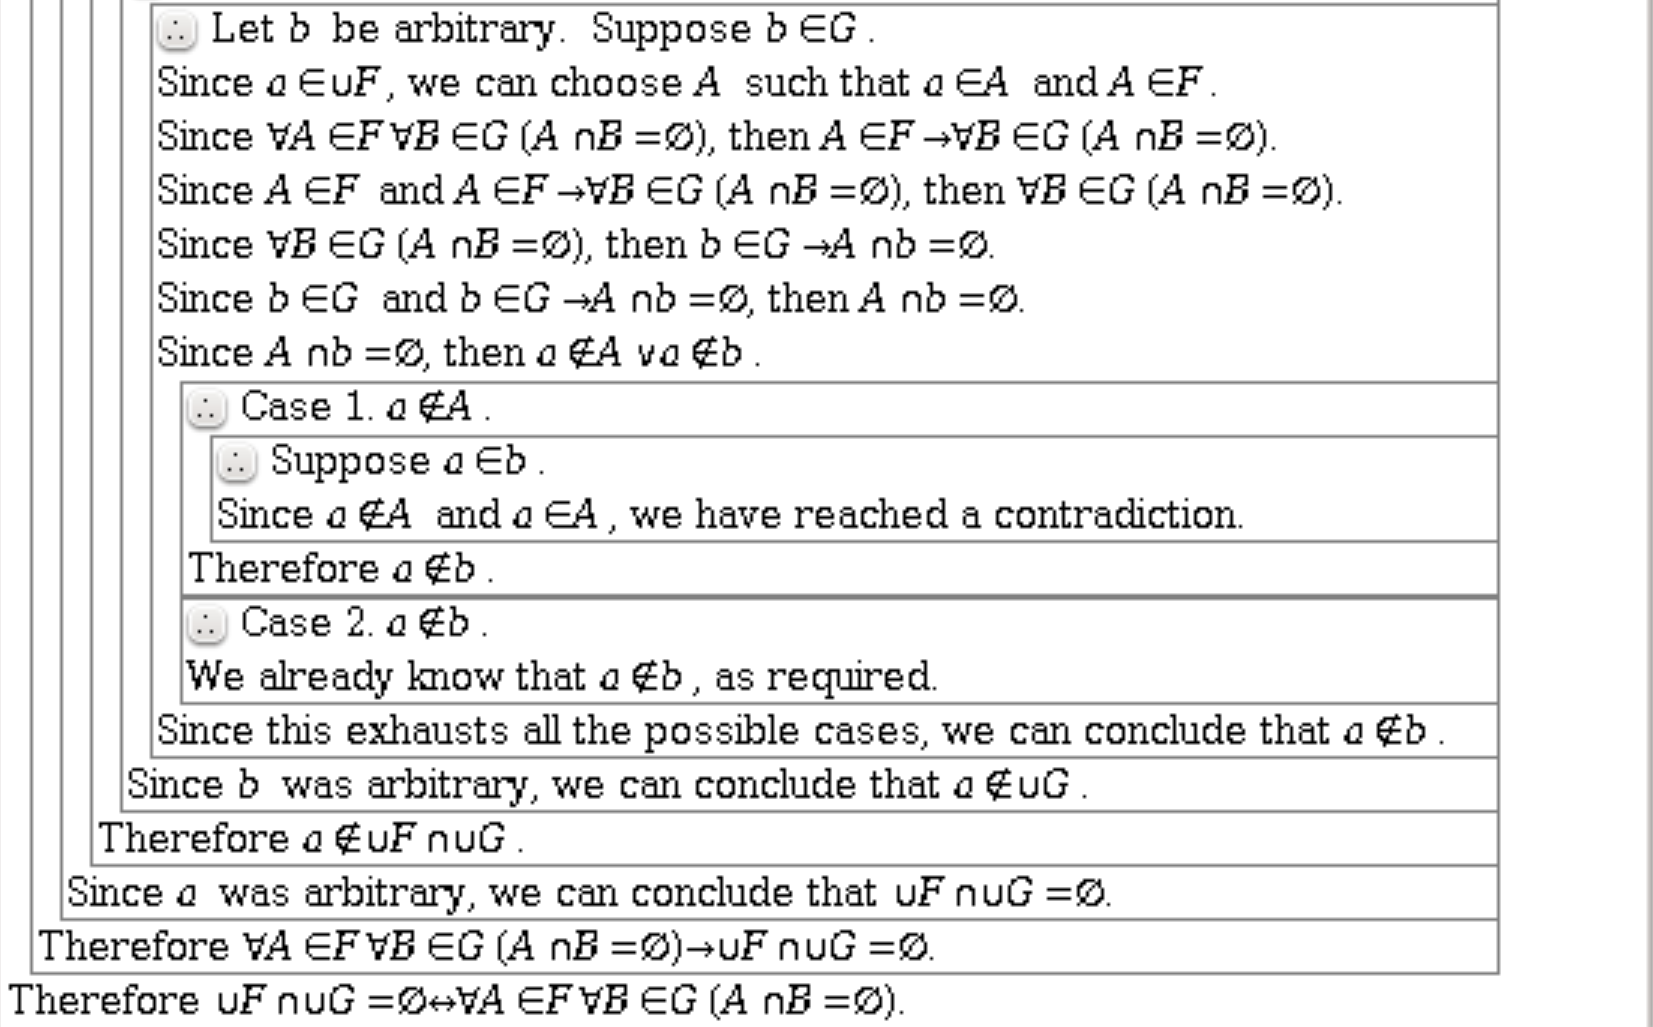
\includegraphics[width=\textwidth]{3_4_20_1}


\vspace{30pt}

(b) "Since $x \in A$ and $A \notin \mathcal{G}$, $x \notin \cup \mathcal{G}$" is wrong prove.

\vspace{30pt}

(c)

\textbf{3.4.20.2.pd}
\vspace{10pt}

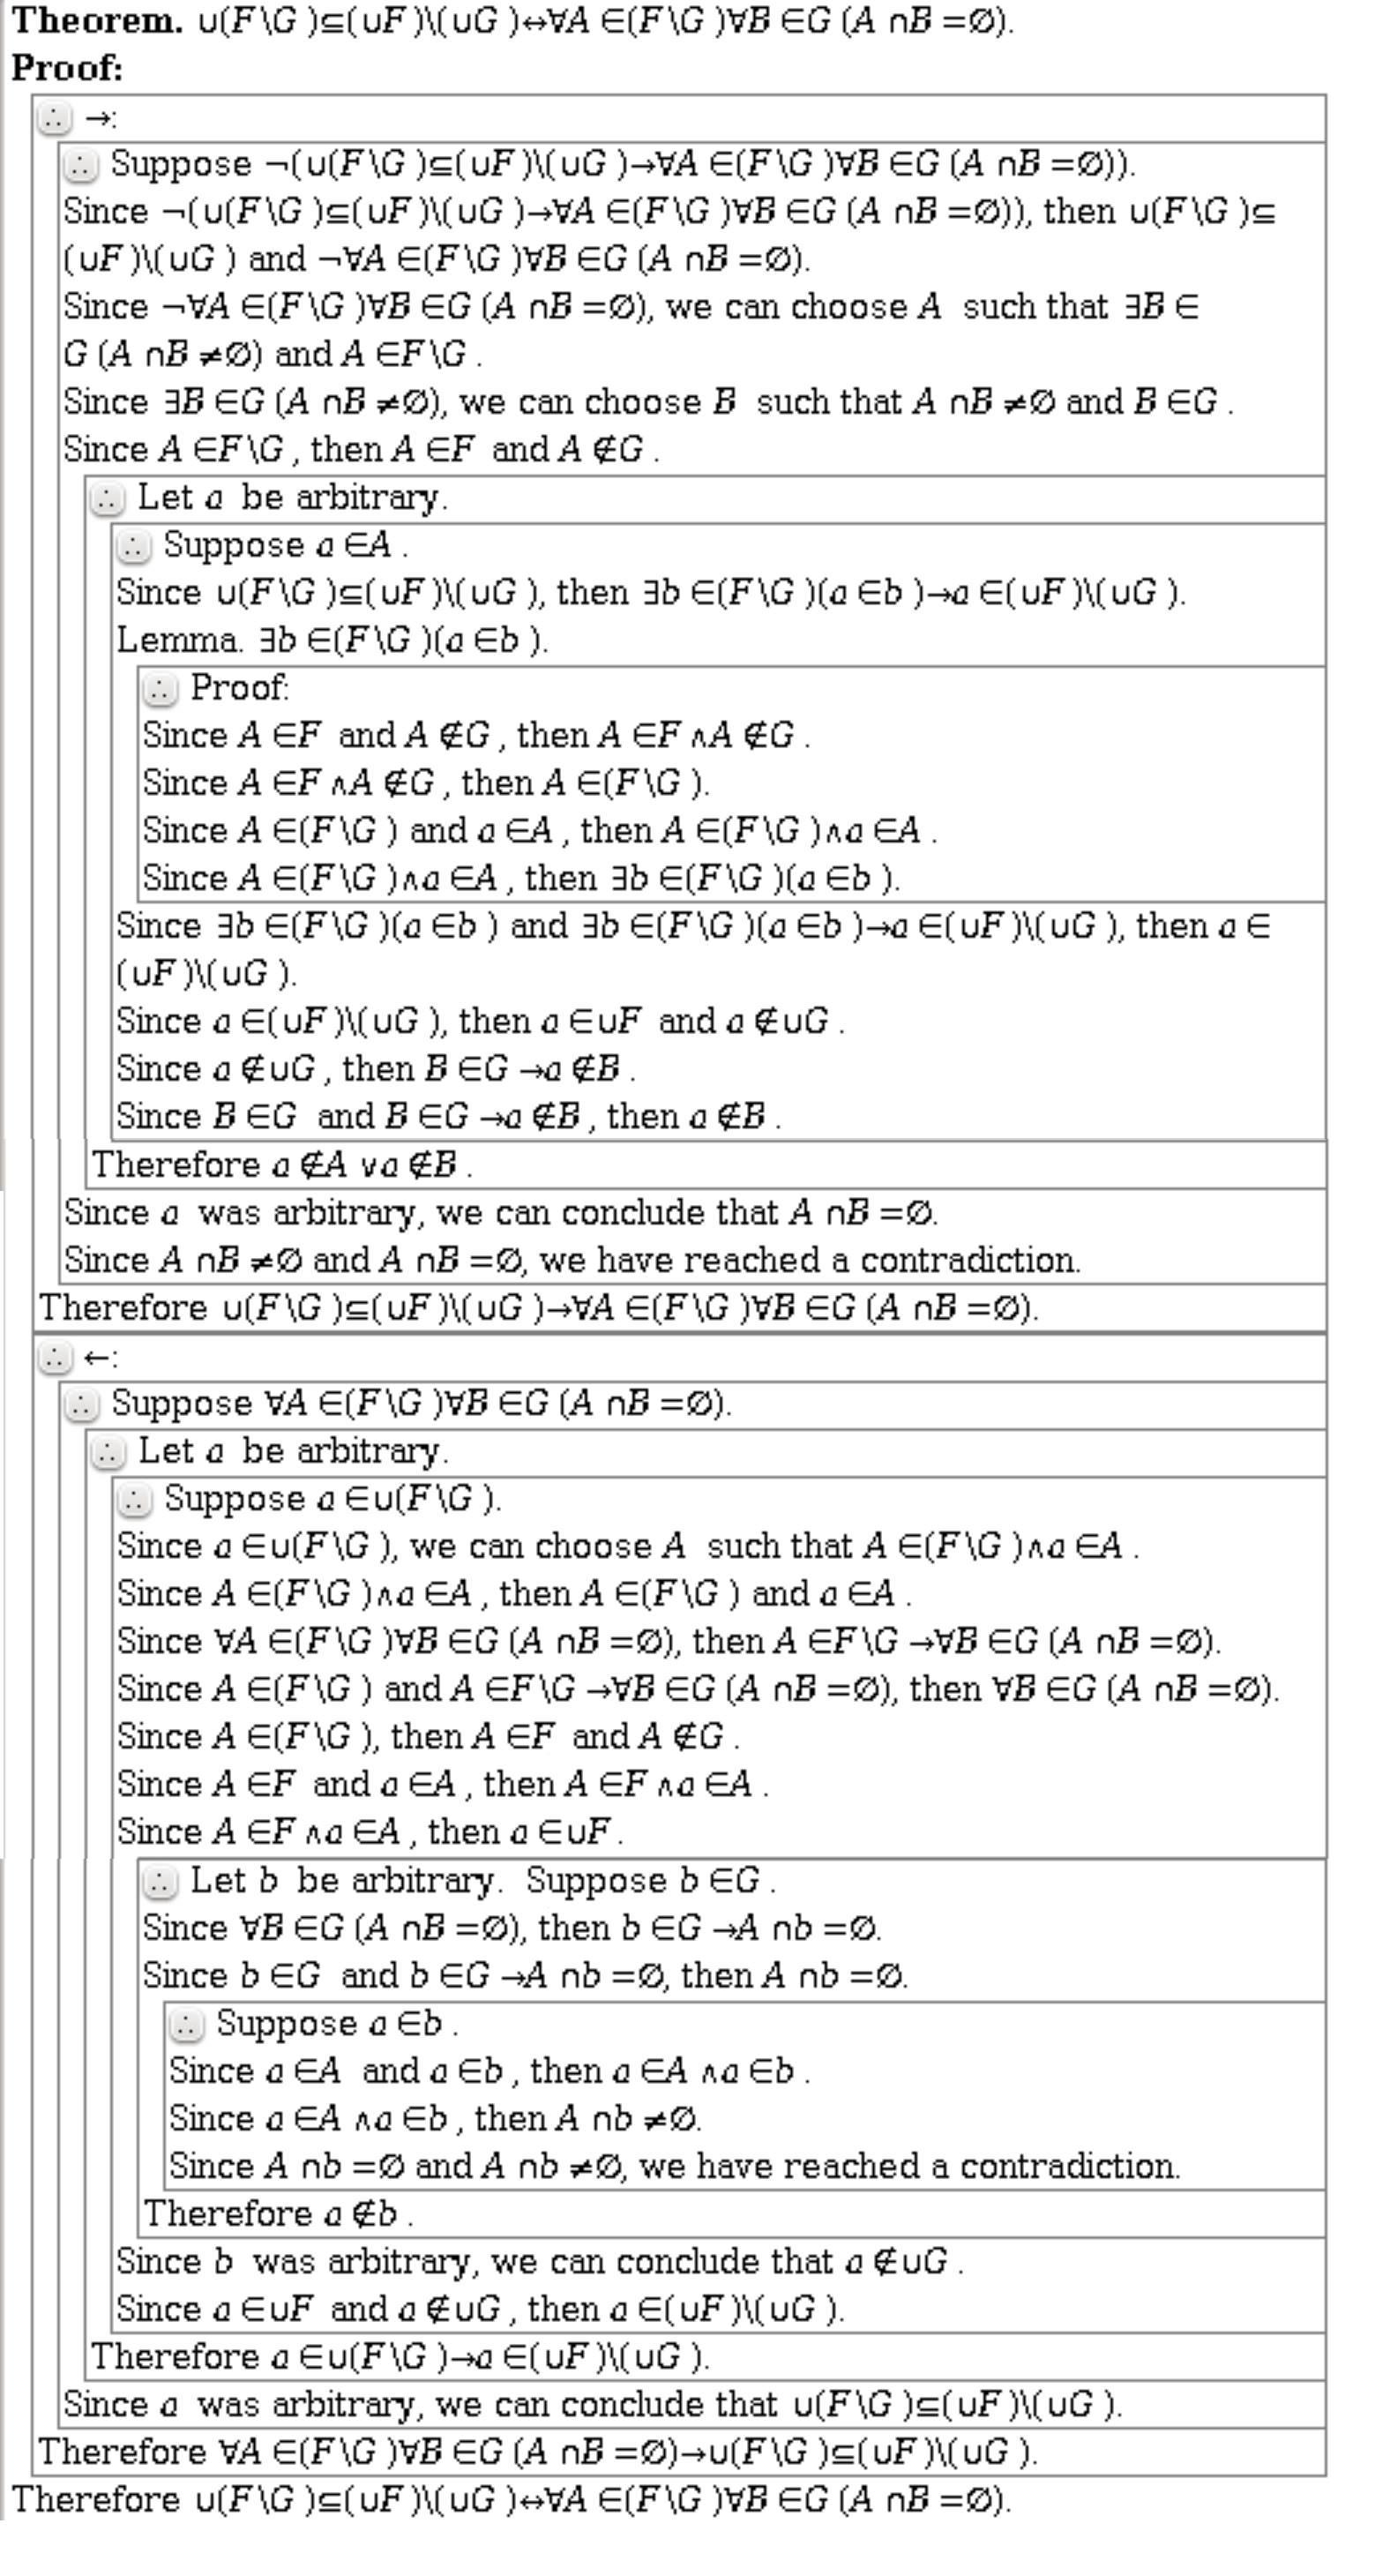
\includegraphics[scale=0.15]{3_4_20_2}

\vspace{30pt}

(d) $\mathcal{F} = \{\{1\}, \{1,2\}\}$

$\mathcal{G} = \{\{1\}, \{2\}\}$

$\cup \mathcal{F} = \{1, 2\}$

$\cup \mathcal{G} = \{1, 2\}$

$(\cup\mathcal{F}) \setminus (\cup\mathcal{G}) = \varnothing$

$\mathcal{F} \setminus \mathcal{G} = \{\{1,2\}\}$

$\cup (\mathcal{F} \setminus \mathcal{G}) = \{1, 2\}$

$\cup (\mathcal{F} \setminus \mathcal{G}) \neq (\cup\mathcal{F}) \setminus (\cup\mathcal{G})$

$\{1,2\} \neq \varnothing$

\vspace{30pt}

$^{\textit{P}}_{\, \textit{D}}$ *21. Suppose $\mathcal{F}$ and $\mathcal{G}$ are families of sets. Prove that if $\cup \mathcal{F} \nsubseteq \cup\mathcal{G}$, then there is some $A \in \mathcal{F}$ such that for all $B \in \mathcal{G}$, $A \nsubseteq B$.
\vspace{30pt}

\textbf{3.4.21.pd}
\vspace{10pt}

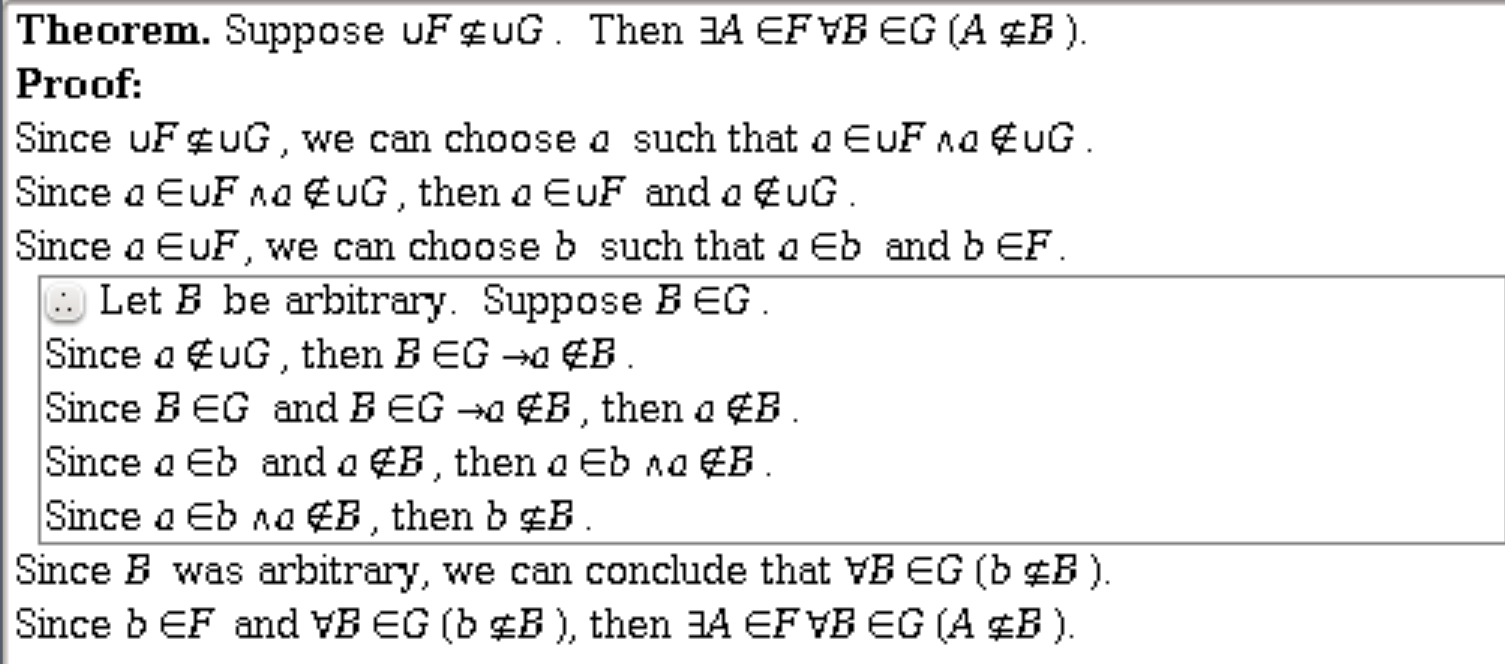
\includegraphics[width=\textwidth]{3_4_21}

\vspace{30pt}

22. Suppose B is a set, $\{A_i \mid i \in I\}$ is an indexed family of sets, and $I \neq \varnothing$.

\hspace{12pt}(a) What proof strategies are used in the following proof that $B \cap
(\cup_{i \in I} A_i) = \cup_{i \in I} (B \cap A_i)$?

\textit{Proof.} Let x be arbitrary. Suppose $x \in B \cap (\cup_{i \in I} A_i)$. Then $x \in B$
and $x \in \cup_{i \in I} A_i$ , so we can choose some $i_0 \in I$ such that $x \in A_{i_0}$ .
Since $x \in B$ and $x \in A_{i_0}$ , $x \in B \cap A_{i_0}$ . Therefore $x \in \cup_{i \in I} (B \cap
A_i)$.

Now suppose $x \in \cup_{i \in I} (B \cap A_i)$. Then we can choose some $i_0 \in
I$ such that $x \in B \cap A_{i_0}$ . Therefore $x \in B$ and $x \in A_{i_0}$ . Since $x \in
A_{i_0}$ , $x \in \cup_{i \in I} A_i$ . Since $x \in B$ and $x \in \cup_{i \in I} A_i$, $x \in B \cap (\cup_{i \in I} A_i)$.

Since x was arbitrary, we have shown that $\forall x[x \in B \cap (\cup_{i \in I} A_i) \leftrightarrow x \in \cup_{i \in I} (B \cap A_i)]$, so $B \cap (\cup_{i \in I} A_i) = \cup_{i \in I} (B \cap A_i)$.

\hspace{12pt}(b) Prove that $B \setminus (\cup_{i \in I} A_i) = \cap_{i \in I} (B \setminus A_i)$.

\hspace{12pt}(c) Can you discover and prove a similar theorem about $B \setminus (\cap_{i \in I} A_i)$?
(Hint: Try to guess the theorem, and then try to prove it. If you can't
finish the proof, it might be because your guess was wrong. Change
your guess and try again.)
\vspace{30pt}

(a)

\centerline{($\rightarrow$)}

\centerline{
  \begin{tabular}{l l}
  \textit{Givens} & \textit{Goal} \\
    $x \in B \cap (\cup_{i \in I} A_i)$ & $x \in \cup_{i \in I} (B \cap A_i)$ \\
 \end{tabular}}
\vspace{10pt}

\centerline{
  \begin{tabular}{l l}
  \textit{Givens} & \textit{Goal} \\
    $x \in B$ & $x \in \cup_{i \in I} (B \cap A_i)$ \\
    $x \in \cup_{i \in I} A_i$ & \\
 \end{tabular}}
\vspace{10pt}

\centerline{
  \begin{tabular}{l l}
  \textit{Givens} & \textit{Goal} \\
    $x \in B$ & $x \in \cup_{i \in I} (B \cap A_i)$ \\
    $\exists i \in I (x \in A_i)$ & \\
 \end{tabular}}
\vspace{10pt}

\centerline{
  \begin{tabular}{l l}
  \textit{Givens} & \textit{Goal} \\
    $x \in B$ & $x \in \cup_{i \in I} (B \cap A_i)$ \\
    $x \in A_{i_0}$ & \\
 \end{tabular}}
\vspace{10pt}

\centerline{
  \begin{tabular}{l l}
  \textit{Givens} & \textit{Goal} \\
    $x \in B \cap A_{i_0}$ & $x \in \cup_{i \in I} (B \cap A_i)$ \\
 \end{tabular}}

\vspace{10pt}
\centerline{
  \begin{tabular}{l l}
  \textit{Givens} & \textit{Goal} \\
    $x \in B \cap A_{i_0}$ & $\exists i \in I (x \in B \cap A_i)$ \\
 \end{tabular}}
\vspace{10pt}

\centerline{($\leftarrow$)}

\centerline{
  \begin{tabular}{l l}
  \textit{Givens} & \textit{Goal} \\
    $x \in \cup_{i \in I} (B \cap A_i)$ & $x \in B \cap (\cup_{i \in I} A_i)$ \\
 \end{tabular}}
\vspace{10pt}

\centerline{
  \begin{tabular}{l l}
  \textit{Givens} & \textit{Goal} \\
    $\exists i \in I (x \in B \cap A_i)$ & $x \in B \cap (\cup_{i \in I} A_i)$ \\
 \end{tabular}}
\vspace{10pt}

\centerline{
  \begin{tabular}{l l}
  \textit{Givens} & \textit{Goal} \\
    $x \in B \land x \in A_{i_0}$ & $x \in B \cap (\cup_{i \in I} A_i)$ \\
 \end{tabular}}
\vspace{10pt}

\centerline{
  \begin{tabular}{l l}
  \textit{Givens} & \textit{Goal} \\
    $x \in B$ & $x \in B \cap (\cup_{i \in I} A_i)$ \\
    $x \in \cup_{i \in I}A_i$ & \\
 \end{tabular}}
\vspace{10pt}

\vspace{30pt}

(b)

\centerline{($\rightarrow$)}

\centerline{
  \begin{tabular}{l l}
  \textit{Givens} & \textit{Goal} \\
    $B \setminus (\cup_{i \in I} A_i)$ & $\cap_{i \in I} (B \setminus A_i)$ \\
 \end{tabular}}
\vspace{10pt}

\centerline{
  \begin{tabular}{l l}
  \textit{Givens} & \textit{Goal} \\
    $B \setminus (\cup_{i \in I} A_i)$ & $\forall i \in I (x \in B \setminus A_i)$ \\
 \end{tabular}}
\vspace{10pt}

\centerline{
  \begin{tabular}{l l}
  \textit{Givens} & \textit{Goal} \\
    $B \setminus (\cup_{i \in I} A_i)$ & $x \in B \land x \notin A_{i_0}$ \\
 \end{tabular}}
\vspace{10pt}

\centerline{
  \begin{tabular}{l l}
  \textit{Givens} & \textit{Goal} \\
    $x \in B$ & $x \in B \land x \notin A_{i_0}$ \\
    $x \notin \cup_{i \in I} A_i$ & \\
 \end{tabular}}
\vspace{10pt}

\centerline{
  \begin{tabular}{l l}
  \textit{Givens} & \textit{Goal} \\
    $x \in B$ & $x \in B \land x \notin A_{i_0}$ \\
    $\neg \exists i \in I (x \in A_i)$ & \\
 \end{tabular}}
\vspace{10pt}

\centerline{
  \begin{tabular}{l l}
  \textit{Givens} & \textit{Goal} \\
    $x \in B$ & $x \in B \land x \notin A_{i_0}$ \\
    $\forall i \in I (x \notin A_i)$ & \\
 \end{tabular}}
\vspace{10pt}

\centerline{
  \begin{tabular}{l l}
  \textit{Givens} & \textit{Goal} \\
    $x \in B$ & $x \in B \land x \notin A_{i_0}$ \\
    $x \notin A_{i_0}$ & \\
 \end{tabular}}
\vspace{10pt}

\centerline{($\leftarrow$)}

\centerline{
  \begin{tabular}{l l}
  \textit{Givens} & \textit{Goal} \\
    $\cap_{i \in I} (B \setminus A_i)$ & $B \setminus (\cup_{i \in I} A_i)$ \\
 \end{tabular}}
\vspace{10pt}

\centerline{
  \begin{tabular}{l l}
  \textit{Givens} & \textit{Goal} \\
    $\forall i \in I (x \in B \setminus A_i)$ & $B \setminus (\cup_{i \in I} A_i)$ \\
 \end{tabular}}
\vspace{10pt}

\centerline{
  \begin{tabular}{l l}
  \textit{Givens} & \textit{Goal} \\
    $\forall i \in I (x \in B \setminus A_i)$ & $B \setminus (\cup_{i \in I} A_i)$ \\
 \end{tabular}}
\vspace{10pt}

$$\forall i \in I (x \in B \setminus A_i)$$
$$\forall i \in I (x \in B) \land \forall i \in I (x \notin A_i)$$
$$x \in B \land \neg \exists i \in I (x \in A_i)$$
$$B \setminus (\cup_{i \in I} A_i)$$
\vspace{20pt}

\textbf{Theorem.} $B \setminus (\cup_{i \in I} A_i) = \cap_{i \in I} (B \setminus A_i)$.

\textit{Proof.} Let x be arbitrary. Let $i_0$ to be arbitrary element from $I$. Suppose $x \in B \setminus (\cup_{i \in I} A_i)$. Then $x \in B$ and $x \notin (\cup_{i \in I} A_i)$. Since $x \notin (\cup_{i \in I} A_i)$, in particular $x \notin A_{i_0}$. Since $x \in B$ and $x \notin A_{i_0}$, $x \in B \land x \notin A_{i_0}$. Since $i_0$ was arbitrary, we have shown that $\forall i \in I (x \in B \setminus A_i)$, so $\cap_{i \in I} (B \setminus A_i)$.

Now suppose $x \in \cap_{i \in I} (B \setminus A_i)$. Since $x \in \cap_{i \in I} (B \setminus A_i)$ then:

$$\forall i \in I (x \in B \setminus A_i)$$
$$\forall i \in I (x \in B) \land \forall i \in I (x \notin A_i)$$
$$x \in B \land \neg \exists i \in I (x \in A_i)$$
$$B \setminus (\cup_{i \in I} A_i)$$.

Thus, $x \in B \setminus (\cup_{i \in I} A_i)$.

Since x was arbitrary, we have shown that $\forall x[x \in (B \setminus (\cup_{i \in I} A_i)) \leftrightarrow x \in \cap_{i \in I} (B \setminus A_i)]$, so $B \setminus (\cup_{i \in I} A_i) = \cap_{i \in I} (B \setminus A_i)$.


\vspace{30pt}

(c) 

$B \setminus (\cap_{i \in I} A_i) = \cup_{i \in I} (B \setminus A_i)$

\centerline{($\rightarrow$)}

\centerline{
  \begin{tabular}{l l}
  \textit{Givens} & \textit{Goal} \\
    $B \setminus (\cap_{i \in I} A_i)$ & $\cup_{i \in I} (B \setminus A_i)$ \\
 \end{tabular}}
\vspace{10pt}

$B \setminus (\cap_{i \in I} A_i)$

$x \in B$

$\neg x \in \cap_{i \in I} A_i$

$\neg \forall i \in I (x \in A_i)$
$\exists i \in I (x \notin A_i)$

\centerline{
  \begin{tabular}{l l}
  \textit{Givens} & \textit{Goal} \\
    $x \in B$ & $\cup_{i \in I} (B \setminus A_i)$ \\
    $\exists i \in I (x \notin A_i)$ & \\
 \end{tabular}}
\vspace{10pt}

$\cup_{i \in I} (B \setminus A_i)$

$\exists i \in I (x \in B \land x \notin A_i)$

\centerline{
  \begin{tabular}{l l}
  \textit{Givens} & \textit{Goal} \\
    $x \in B$ & $\exists i \in I (x \in B \land x \notin A_i)$ \\
    $\exists i \in I (x \notin A_i)$ & \\
 \end{tabular}}
\vspace{10pt}

\centerline{
  \begin{tabular}{l l}
  \textit{Givens} & \textit{Goal} \\
    $x \in B$ & $\exists i \in I (x \in B \land x \notin A_i)$ \\
    $i \in I$ & \\
    $x \notin A_i$ & \\
 \end{tabular}}
\vspace{10pt}

\centerline{($\leftarrow$)}

\centerline{
  \begin{tabular}{l l}
  \textit{Givens} & \textit{Goal} \\
    $\cup_{i \in I} (B \setminus A_i)$ & $B \setminus (\cap_{i \in I} A_i)$ \\
 \end{tabular}}
\vspace{10pt}

\centerline{
  \begin{tabular}{l l}
  \textit{Givens} & \textit{Goal} \\
    $\exists i \in I (x \in B \land x \notin A_i)$ & $x \in B \land \exists i \in I (x \notin A_i)$ \\
 \end{tabular}}
\vspace{10pt}

\centerline{
  \begin{tabular}{l l}
  \textit{Givens} & \textit{Goal} \\
    $x \in B \land x \notin A_i$ & $x \in B \land \exists i \in I (x \notin A_i)$ \\
    $i \in I$ & \\
 \end{tabular}}
\vspace{20pt}

\textbf{Theorem.} $B \setminus (\cap_{i \in I} A_i) = \cup_{i \in I} (B \setminus A_i)$

\textit{Proof.} Suppose $B \setminus (\cap_{i \in I} A_i)$. Then $x \in B$ and $x \notin \cap_{i \in I} A_i$. Since $x \notin \cap_{i \in I} A_i$, we can choose some $i \in I$ such that $x \notin A_i$. Since $x \in B$ and $x \notin A_i$, $x \in B \setminus A_i$. Since $x \in B \setminus A_i$, $\cup_{i \in I} (B \setminus A_i)$.

Now suppose $\cup_{i \in I} (B \setminus A_i)$. Then, we can choose some $i \in I$ such that $x \in B$ and $x \notin A_i$. Since $x \notin A_i$, $x \notin \cap_{i \in I} A_i$. Therefore, $B \setminus (\cap_{i \in I} A_i)$.

Thus, $B \setminus (\cap_{i \in I} A_i) = \cup_{i \in I} (B \setminus A_i)$.

\vspace{30pt}

*23. Suppose $\{A_i \mid i \in I\}$ and $\{B_i \mid i \in I\}$ are indexed families of sets and
$I \neq \varnothing$.

\hspace{12pt}(a) Prove that $\cup_{i \in I} (A_i \setminus B_i) \subseteq (\cup_{i \in I} A_i) \setminus (\cap_{i \in I} B_i)$.

\hspace{12pt}(b) Find an example for which $\cup_{i \in I} (A_i \setminus B_i) \neq (\cup_{i \in I} A_i) \setminus (\cap_{i \in I} B_i)$.
\vspace{30pt}

(a)

\centerline{
  \begin{tabular}{l l}
  \textit{Givens} & \textit{Goal} \\
    $$ & $\cup_{i \in I} (A_i \setminus B_i) \subseteq (\cup_{i \in I} A_i) \setminus (\cap_{i \in I} B_i)$ \\
 \end{tabular}}
\vspace{10pt}

\centerline{
  \begin{tabular}{l l}
  \textit{Givens} & \textit{Goal} \\
    $$ & $\forall x (x \in \cup_{i \in I} (A_i \setminus B_i) \to x \in (\cup_{i \in I} A_i) \setminus (\cap_{i \in I} B_i))$ \\
 \end{tabular}}
\vspace{10pt}

Let x be arbitrary

\centerline{
  \begin{tabular}{l l}
  \textit{Givens} & \textit{Goal} \\
    $$ & $x \in \cup_{i \in I} (A_i \setminus B_i) \to x \in (\cup_{i \in I} A_i) \setminus (\cap_{i \in I} B_i)$ \\
 \end{tabular}}
\vspace{10pt}

Suppose $x \in \cup_{i \in I} (A_i \setminus B_i)$

\centerline{
  \begin{tabular}{l l}
  \textit{Givens} & \textit{Goal} \\
    $x \in \cup_{i \in I} (A_i \setminus B_i)$ & $x \in (\cup_{i \in I} A_i) \setminus (\cap_{i \in I} B_i)$ \\
 \end{tabular}}
\vspace{10pt}

$x \in \cup_{i \in I} (A_i \setminus B_i)$

$\exists i \in I (x \in A_i \setminus B_i)$

\centerline{
  \begin{tabular}{l l}
  \textit{Givens} & \textit{Goal} \\
    $x \in A_i$ & $x \in (\cup_{i \in I} A_i) \setminus (\cap_{i \in I} B_i)$ \\
    $x \notin B_i$ & \\
    $i \in I$ & \\
 \end{tabular}}
\vspace{10pt}

$x \in (\cup_{i \in I} A_i) \setminus (\cap_{i \in I} B_i)$

$x \in (\cup_{i \in I} A_i) \land \neg x \in (\cap_{i \in I} B_i)$

$\exists i \in I (x \in A_i) \land \exists i \in I (x \notin B_i)$

\centerline{
  \begin{tabular}{l l}
  \textit{Givens} & \textit{Goal} \\
    $x \in A_i$ & $\exists i \in I (x \in A_i) \land \exists i \in I (x \notin B_i)$ \\
    $x \notin B_i$ & \\
    $i \in I$ & \\
  \end{tabular}}
\vspace{10pt}

\textbf{Theorem.} $\cup_{i \in I} (A_i \setminus B_i) \subseteq (\cup_{i \in I} A_i) \setminus (\cap_{i \in I} B_i)$

\textit{Proof.} Let x be arbitrary.
Suppose $x \in \cup_{i \in I} (A_i \setminus B_i)$.
Then we can choose some $i \in I$ such that $x \in A_i \setminus B_i$. Since $x \in A$, $x \in \cup_{i \in I}A_i$ and since $x \notin B_i$, $x \notin \cap_{i \in I}B_i$. Therefore $x \in (\cup_{i \in I} A_i) \setminus (\cap_{i \in I} B_i)$. 
Since x was arbitrary, we proved that $\forall x (x \in \cup_{i \in I} (A_i \setminus B_i) \to x \in (\cup_{i \in I} A_i) \setminus (\cap_{i \in I} B_i))$, so $\cup_{i \in I} (A_i \setminus B_i) \subseteq (\cup_{i \in I} A_i) \setminus (\cap_{i \in I} B_i)$

\vspace{30pt}

(b) 

$I = \{1,2\}$

$A_1 = \{1\}$ $A_2 = \{1,2\}$

$B_1 = \{1,2\}$ $B_2 = \{1,2\}$

$\cup_{i \in I} (A_i \setminus B_i) \neq (\cup_{i \in I} A_i) \setminus (\cap_{i \in I} B_i)$

$\cup_{i \in I} (A_i \setminus B_i) = \{1\}$
\vspace{10pt}

$(\cup_{i \in I} A_i) \setminus (\cap_{i \in I} B_i) = \{1,2\} \setminus \{1,2\} = \varnothing$

\vspace{30pt}

24. Suppose $\{A_i \mid i \in I\}$ and $\{B_i \mid i \in I\}$ are indexed families of sets.

\hspace{12pt}(a) Prove that $\cup_{i \in I} (A_i \cap B_i) \subseteq (\cup_{i \in I} A_i) \cap (\cup_{i \in I} B_i)$.

\hspace{12pt}(b) Find an example for which $\cup_{i \in I} (A_i \cap B_i) \neq (\cup_{i \in I} A_i) \cap (\cup_{i \in I} B_i)$.
\vspace{30pt}

(a)

\centerline{
  \begin{tabular}{l l}
  \textit{Givens} & \textit{Goal} \\
    $$ & $\cup_{i \in I} (A_i \cap B_i) \subseteq (\cup_{i \in I} A_i) \cap (\cup_{i \in I} B_i)$ \\
  \end{tabular}}
\vspace{10pt}

\centerline{
  \begin{tabular}{l l}
  \textit{Givens} & \textit{Goal} \\
    $\cup_{i \in I} (A_i \cap B_i)$ & $(\cup_{i \in I} A_i) \cap (\cup_{i \in I} B_i)$ \\
  \end{tabular}}
\vspace{10pt}

$\cup_{i \in I} (A_i \cap B_i)$

$\exists i \in I (x \in A_i \land x \in B_i)$

\centerline{
  \begin{tabular}{l l}
  \textit{Givens} & \textit{Goal} \\
    $i \in I$ & $(\cup_{i \in I} A_i) \cap (\cup_{i \in I} B_i)$ \\
    $x \in A_i$ & \\
    $x \in B_i$ & \\
  \end{tabular}}
\vspace{10pt}

$(\cup_{i \in I} A_i) \cap (\cup_{i \in I} B_i)$

$\exists i \in I (x \in A_i) \land \exists i \in I (x \in B_i)$

\centerline{
  \begin{tabular}{l l}
  \textit{Givens} & \textit{Goal} \\
    $i \in I$ & $\exists i \in I (x \in A_i) \land \exists i \in I (x \in B_i)$ \\
    $x \in A_i$ & \\
    $x \in B_i$ & \\
  \end{tabular}}
\vspace{20pt}

\textbf{Theorem.} $\cup_{i \in I} (A_i \cap B_i) \subseteq (\cup_{i \in I} A_i) \cap (\cup_{i \in I} B_i)$

\textit{Proof.} Suppose $\cup_{i \in I} (A_i \cap B_i)$.
Then we can choose some $i \in I$ such that $x \in A_i \cap B_i$,
which means $x \in A_i$ and $x \in B_i$. Since $x \in A_i$, $x \in \cup_{i \in I} A_i$ and since $x \in B_i$, $x \in \cup_{i \in I} B_i$. Therefore,
$(\cup_{i \in I} A_i) \cap (\cup_{i \in I} B_i)$.

\vspace{30pt}

(b)

$I = \{1,2\}$

$A_1 = \{1\}$ $A_2 = \{1,2\}$

$B_1 = \{1\}$ $B_2 = \{2\}$

$\cup_{i \in I} (A_i \cap B_i) \neq (\cup_{i \in I} A_i) \cap (\cup_{i \in I} B_i)$

$\cup_{i \in I} (A_i \cap B_i) = \{1\}$

$(\cup_{i \in I} A_i) \cap (\cup_{i \in I} B_i) = \{1,2\}$

\vspace{30pt}

25. Prove that for all integers a and b there is an integer c such that $a \mid c$ and $b \mid c$.
\vspace{30pt}

\centerline{
  \begin{tabular}{l l}
  \textit{Givens} & \textit{Goal} \\
    $$ & $\forall a \in \mathbb{Z} \forall b \in \mathbb{Z} \exists c \in \mathbb{Z} (a \mid c \text{ and } b \mid c)$ \\
  \end{tabular}}
\vspace{20pt}

\centerline{
  \begin{tabular}{l l}
  \textit{Givens} & \textit{Goal} \\
    $$ & $\exists c \in \mathbb{Z} (a \mid c \text{ and } b \mid c)$ \\
  \end{tabular}}
\vspace{20pt}

$a \mid c = \exists k (ka = c)$

\centerline{
  \begin{tabular}{l l}
  \textit{Givens} & \textit{Goal} \\
    $$ & $\exists c \in \mathbb{Z} (\exists k (ka = c) \land \exists m (mb = c))$ \\
  \end{tabular}}
\vspace{20pt}

\textbf{Theorem.} For all integers a and b there is an integer c such that $a \mid c$ and $b \mid c$.

\textit{Proof.} Let c = 0. Let k = 0. Let m = 0. Then,

$k*a = c$

$0*a = 0$
\vspace{10pt}

$m*b = c$

$0*b = 0$

Therefore, $\exists c \in \mathbb{Z} (a \mid c \text{ and } b \mid c)$.

\vspace{30pt}

26. (a) Prove that for every integer n, $15 \mid n$ iff $3 \mid n$ and $5 \mid n$.

\hspace{12pt}(b) Prove that it is not true that for every integer n, $60 \mid n$ iff $6 \mid n$ and
$10 \mid n$.
\vspace{30pt}

(a) 

\centerline{
  \begin{tabular}{l l}
  \textit{Givens} & \textit{Goal} \\
    $$ & $\forall n \in \mathbb{Z}(15 \mid n \text{ iff } 3 \mid n \text{ and } 5 \mid n)$ \\
  \end{tabular}}
\vspace{20pt}

\centerline{
  \begin{tabular}{l l}
  \textit{Givens} & \textit{Goal} \\
    $$ & $15 \mid n \text{ iff } 3 \mid n \text{ and } 5 \mid n$ \\
  \end{tabular}}
\vspace{20pt}

\centerline{($\rightarrow$)}

\centerline{
  \begin{tabular}{l l}
  \textit{Givens} & \textit{Goal} \\
    $15 \mid n$ & $3 \mid n \text{ and } 5 \mid n$ \\
  \end{tabular}}
\vspace{20pt}

\centerline{
  \begin{tabular}{l l}
  \textit{Givens} & \textit{Goal} \\
    $\exists k (15 k = n)$ & $\exists m (3 m = n) \land \exists p (5 p = n)$ \\
  \end{tabular}}
\vspace{20pt}

\centerline{
  \begin{tabular}{l l}
  \textit{Givens} & \textit{Goal} \\
    $15 k = n$ & $\exists m (3 m = n) \land \exists p (5 p = n)$ \\
    $k \in \mathbb{Z}$ & \\
  \end{tabular}}
\vspace{20pt}

$3(5k) = n$

$m = 5k$

$5(3k) = n$

$p = 3k$

\centerline{($\leftarrow$)}

\centerline{
  \begin{tabular}{l l}
  \textit{Givens} & \textit{Goal} \\
     $3 \mid n \text{ and } 5 \mid n$ & $15 \mid n$ \\
  \end{tabular}}
\vspace{20pt}

\centerline{
  \begin{tabular}{l l}
  \textit{Givens} & \textit{Goal} \\
     $\exists m (3 m = n) \land \exists p (5 p = n)$ & $\exists k (15k = n)$ \\
  \end{tabular}}
\vspace{20pt}

\centerline{
  \begin{tabular}{l l}
  \textit{Givens} & \textit{Goal} \\
    $\exists m (3 m = n)$ & $\exists k (15k = n)$ \\
    $\exists p (5 p = n)$ & \\
  \end{tabular}}
\vspace{20pt}

\centerline{
  \begin{tabular}{l l}
  \textit{Givens} & \textit{Goal} \\
    $3 m = n$ & $\exists k (15k = n)$ \\
    $5 p = n$ & \\
  \end{tabular}}
\vspace{20pt}

\url{http://www.math.uconn.edu/~kconrad/blurbs/ugradnumthy/divgcd.pdf}

\vspace{30pt}

\textbf{Theorem.} For every integer n, $15 \mid n$ iff $3 \mid n$ and $5 \mid n$.

\textit{Proof.} Let n be arbitrary integer.
Suppose $15 \mid n$. Then we can choose some $k \in \mathbb{Z}$ such that
$15k = n$. Since $3 \mid n$, $\exists m (3m = n)$. Let $m = 5k$ then $15k = n$, thus $3 \mid n$. Since $5 \mid n$, $\exists p (5p = n)$. Let $p = 3k$ then $15k = n$, thus $5 \mid n$. Thus, $3 \mid n$ and $5 \mid n$.

Now suppose $3 \mid n \text{ and } 5 \mid n$. Then we can choose some
$m \in \mathbb{Z}$ such that $3m = n$ and some $p \in \mathbb{Z}$ such that $5p = n$. Since $3 \mid n$, $\exists k (15k = n)$. Since $(3, 5) = 1$ we have $3x+5y=1$ for some integer x and y. Therefore

$$n = n*1 = 3nx+5ny=(5p)3x+(3m)5y=15(px+my)$$.

Since $px+my \in \mathbb{Z}$, $15 \mid n$.

Since n was arbitrary integer, $\forall n \in \mathbb{Z}(15 \mid n \leftrightarrow 3 \mid n \text{ and } 5 \mid n)$


(b) Counterexample: $n = 330$

$6 \mid 330$ and $10 \mid 330$ is true, but $60 \mid 330$ is false.


\vspace{50pt}

\textbf{3.5. Proofs Involving Disjunctions}

Exercises:
\vspace{30pt}

$^{\textit{P}}_{\, \textit{D}}$ *1. Suppose A, B, and C are sets. Prove that $A \cap (B \cup C) \subseteq (A \cap B) \cup C$.
\vspace{30pt}

\textbf{3.5.1.pd}
\vspace{10pt}

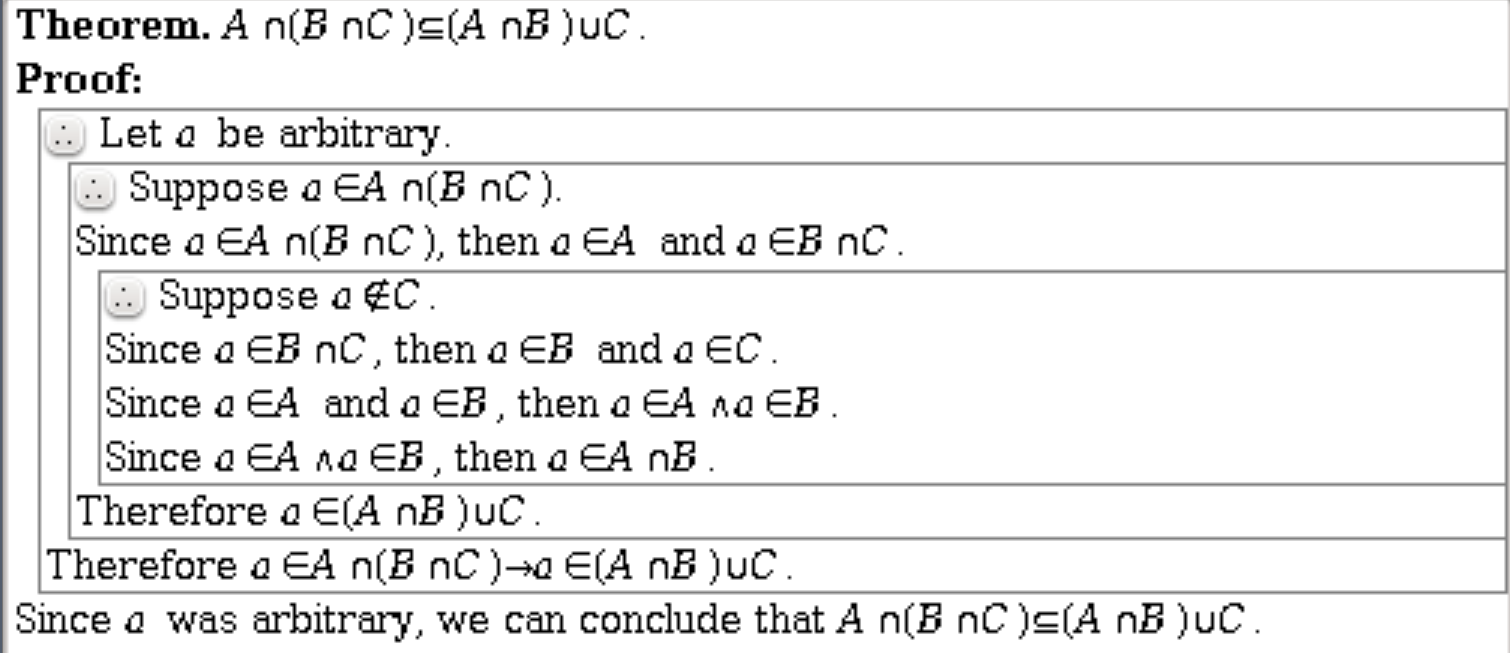
\includegraphics[width=\textwidth]{3_5_1}

\vspace{30pt}

$^{\textit{P}}_{\, \textit{D}}$ 2. Suppose A, B, and C are sets. Prove that $(A \cup B) \setminus C \subseteq A \cup (B \setminus C)$.

\vspace{30pt}

\textbf{3.5.2.pd}
\vspace{10pt}

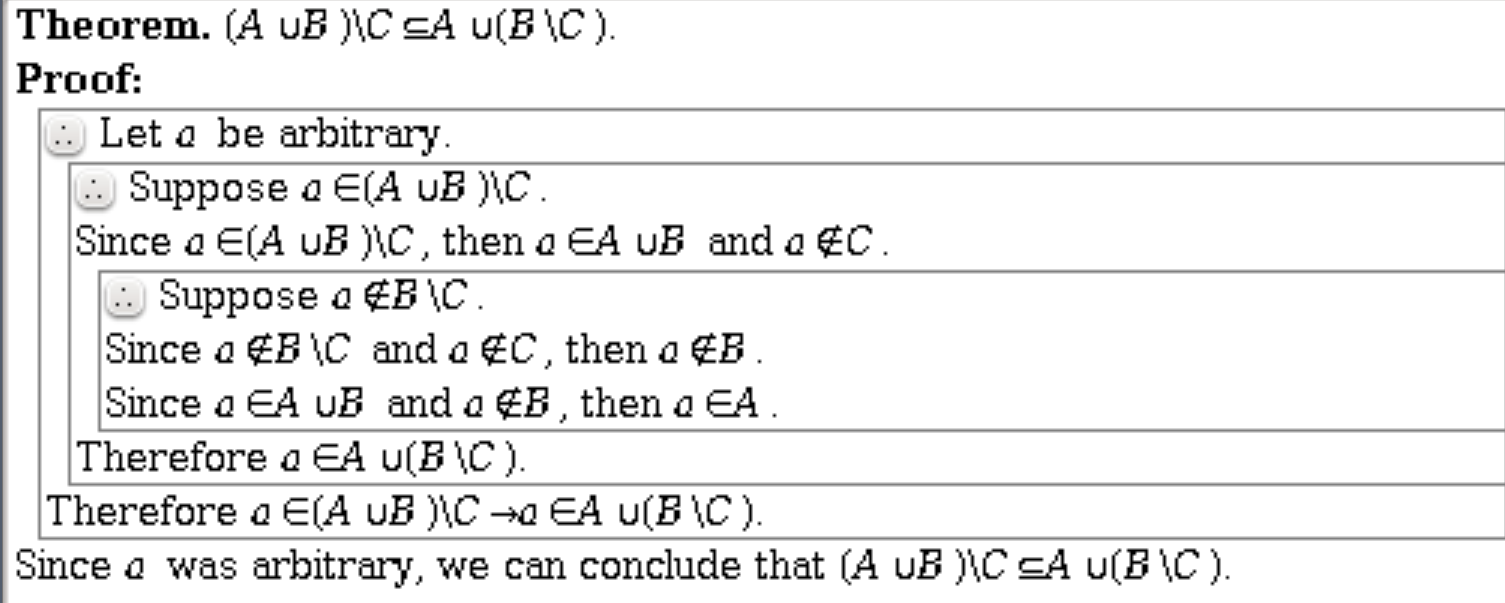
\includegraphics[width=\textwidth]{3_5_2}

\vspace{30pt}

$^{\textit{P}}_{\, \textit{D}}$ 3. Suppose A and B are sets. Prove that $A \setminus (A \setminus B) = A \cap B$.

\vspace{30pt}

\textbf{3.5.3.pd}
\vspace{10pt}

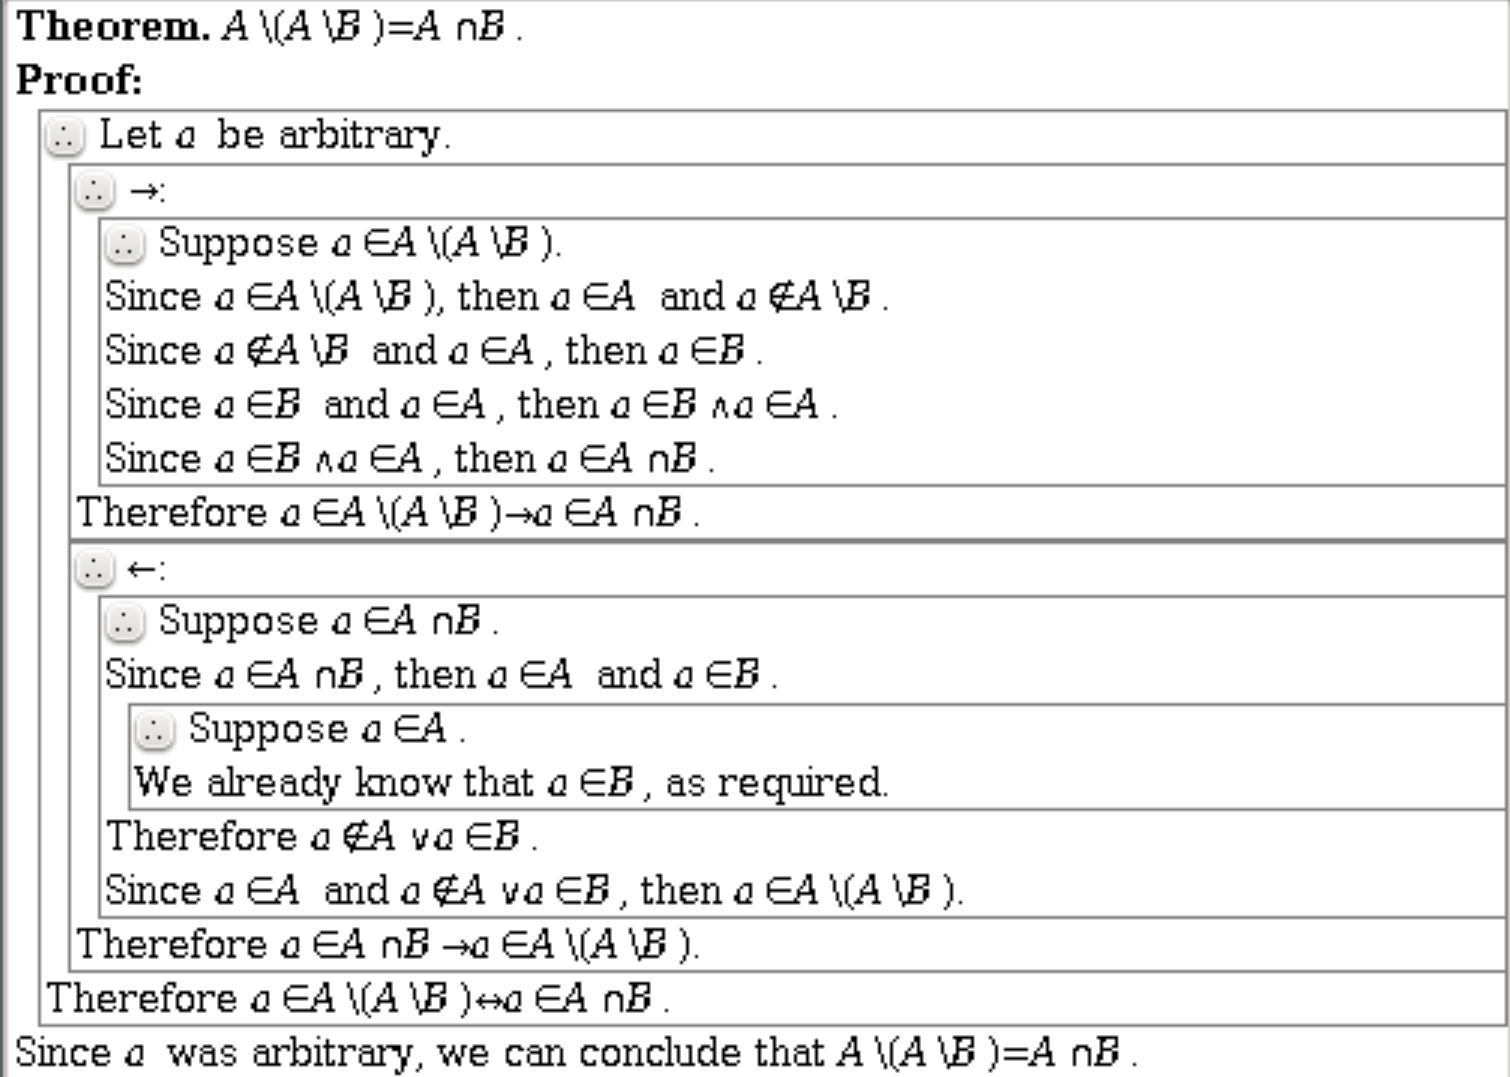
\includegraphics[width=\textwidth]{3_5_3}

\vspace{30pt}

$^{\textit{P}}_{\, \textit{D}}$ *4. Suppose $A \cap C \subseteq B \cap C$ and $A \cup C \subseteq B \cup C$. Prove that $A \subseteq B$.

\vspace{30pt}

\textbf{3.5.4.pd}
\vspace{10pt}

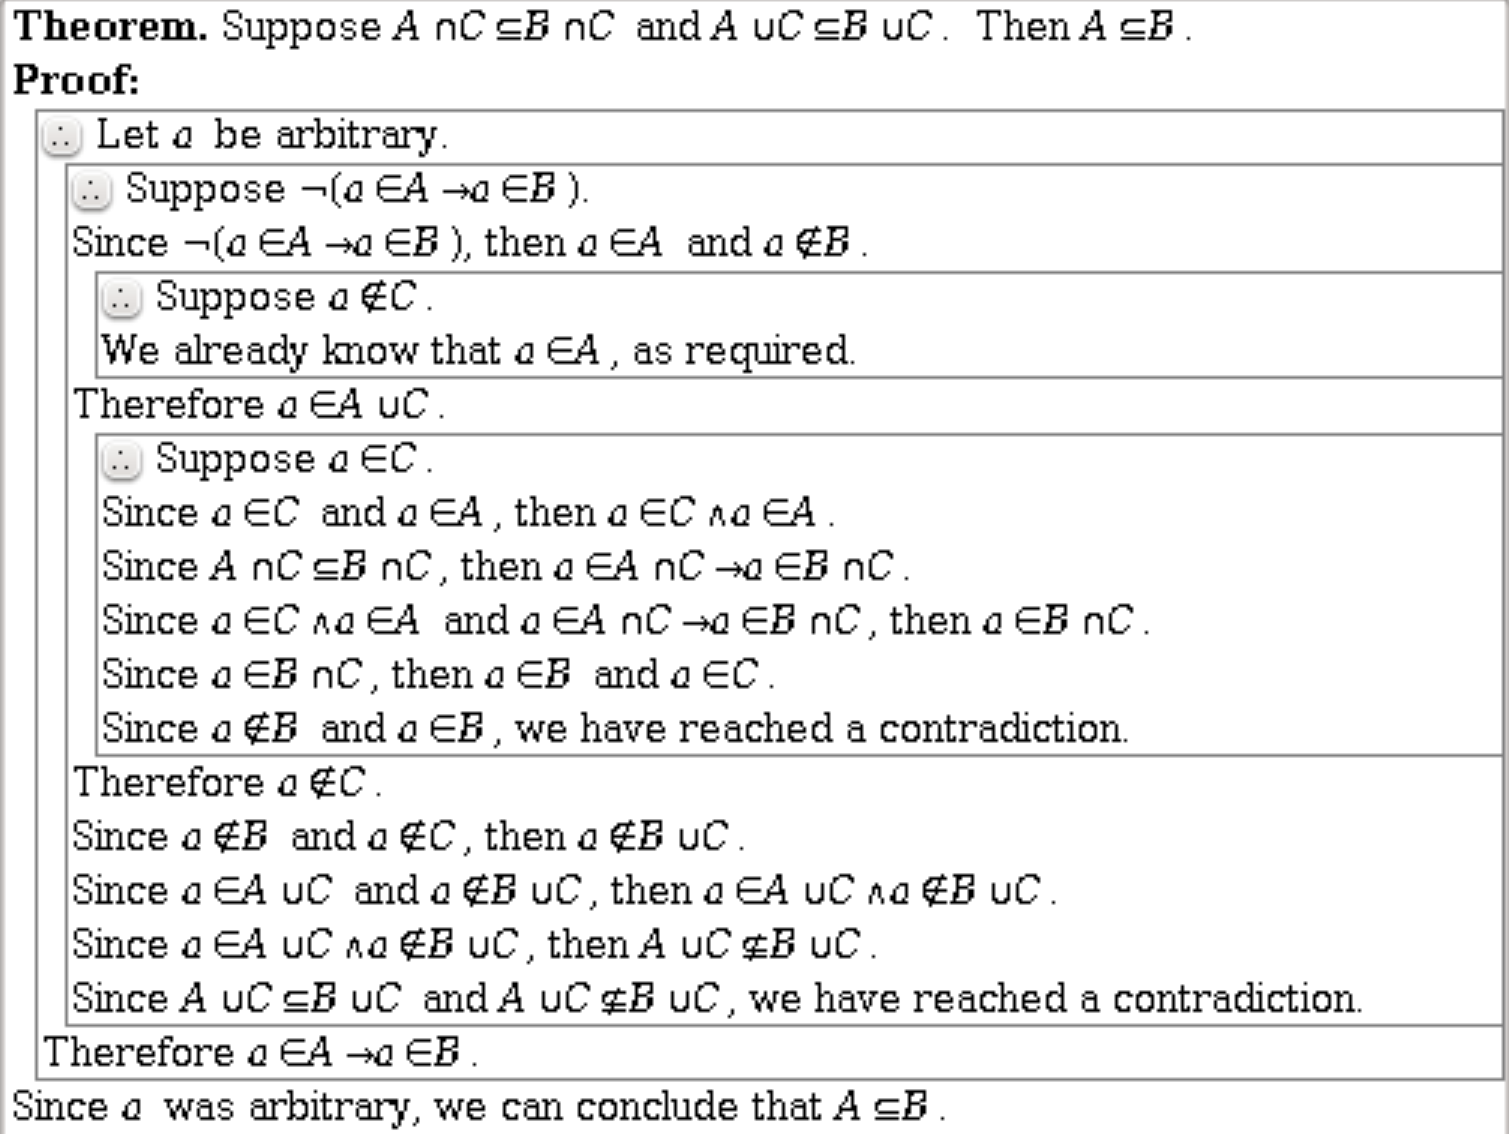
\includegraphics[width=\textwidth]{3_5_4}

\vspace{30pt}

$^{\textit{P}}_{\, \textit{D}}$ 5. Recall from Section 1.4 that the symmetric difference of two sets A and B
is the set $A \Delta B = (A \setminus B) \cup (B \setminus A) = (A \cup B) \setminus (A \cap B)$. Prove that
if $A \Delta B \subseteq A$ then $B \subseteq A$.

\vspace{30pt}

\textbf{3.5.5.pd}
\vspace{10pt}

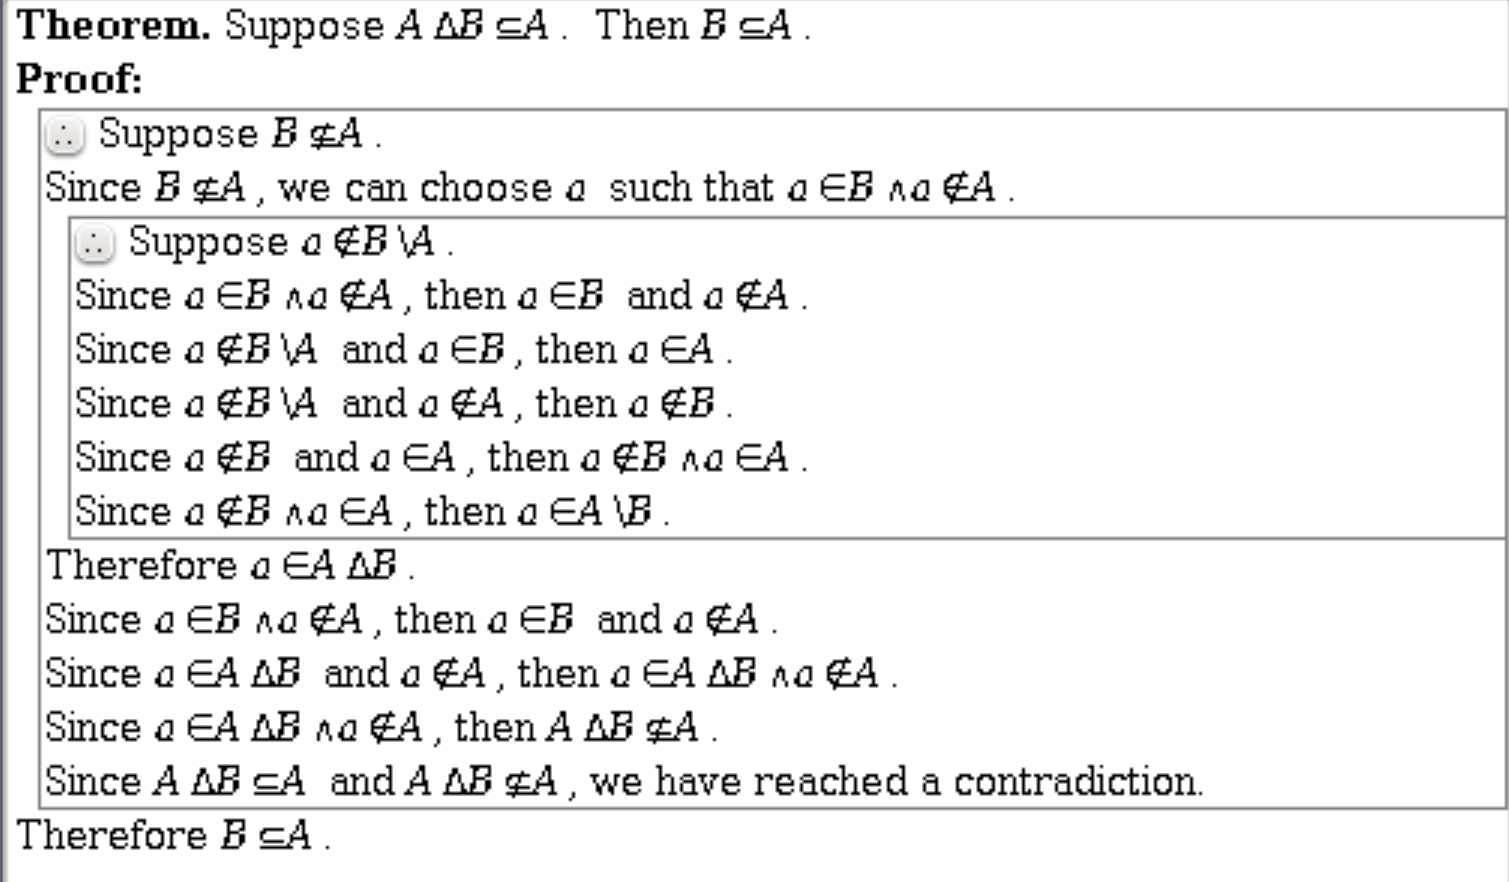
\includegraphics[width=\textwidth]{3_5_5}

\vspace{30pt}

$^{\textit{P}}_{\, \textit{D}}$ 6. Suppose A, B, and C are sets. Prove that $A \cup C \subseteq B \cup C$ iff $A \setminus C \subseteq B \setminus C$.

\vspace{30pt}

\textbf{3.5.6.pd}
\vspace{10pt}

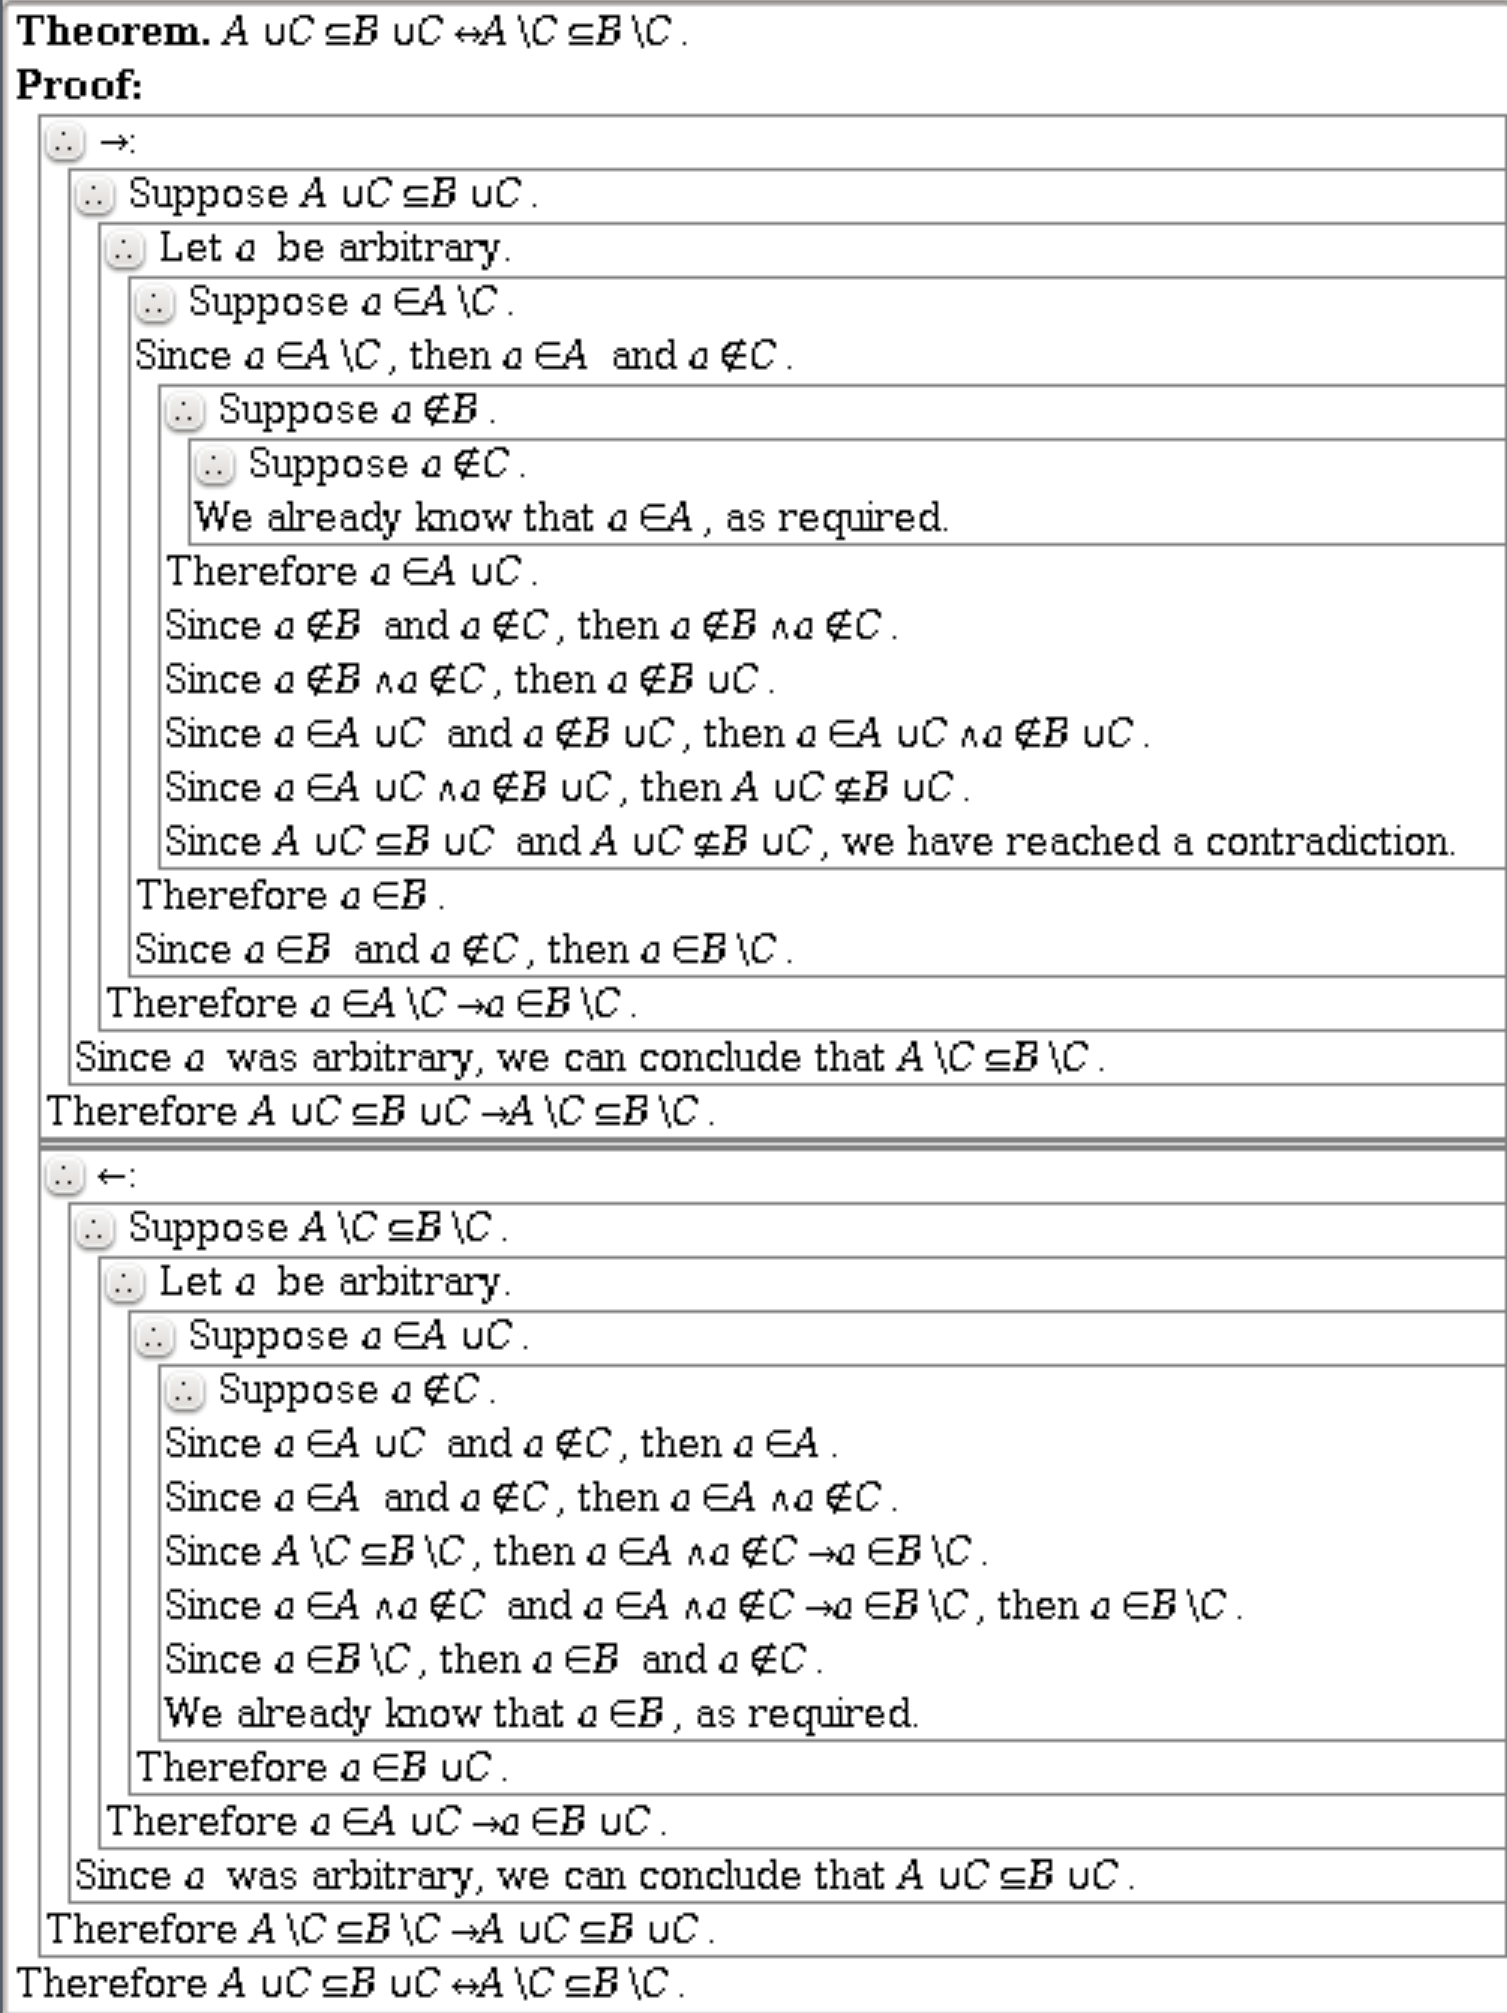
\includegraphics[scale=0.15]{3_5_6}

\vspace{30pt}

$^{\textit{P}}_{\, \textit{D}}$ *7. Prove that for any sets A and B, $\mathcal{P} (A) \cup \mathcal{P} (B) \subseteq \mathcal{P} (A \cup B)$.

\vspace{30pt}

\textbf{3.5.7.pd}
\vspace{10pt}

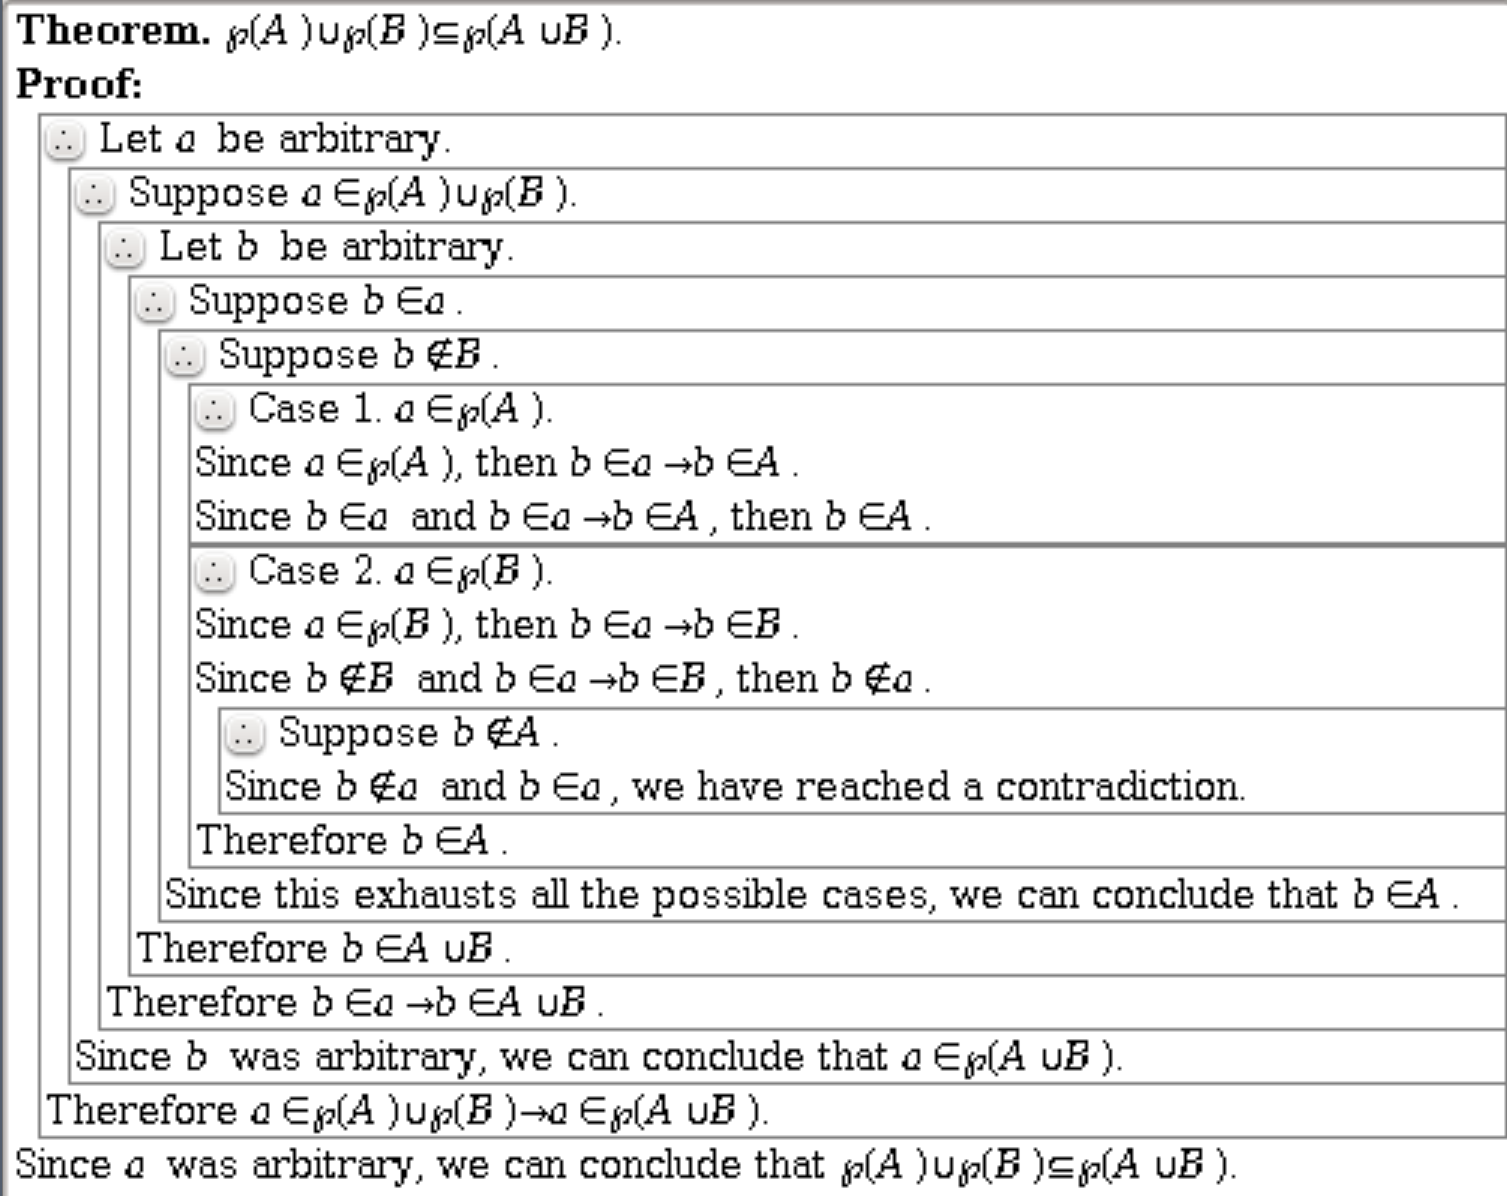
\includegraphics[width=\textwidth]{3_5_7}

\vspace{30pt}

$^{\textit{P}}_{\, \textit{D}}$ 8. Prove that for any sets A and B, if $\mathcal{P} (A) \cup \mathcal{P} (B) = \mathcal{P} (A \cup B)$ then either $A \subseteq B$ or $B \subseteq A$.

\vspace{30pt}

\textbf{3.5.8.pd}
\vspace{10pt}

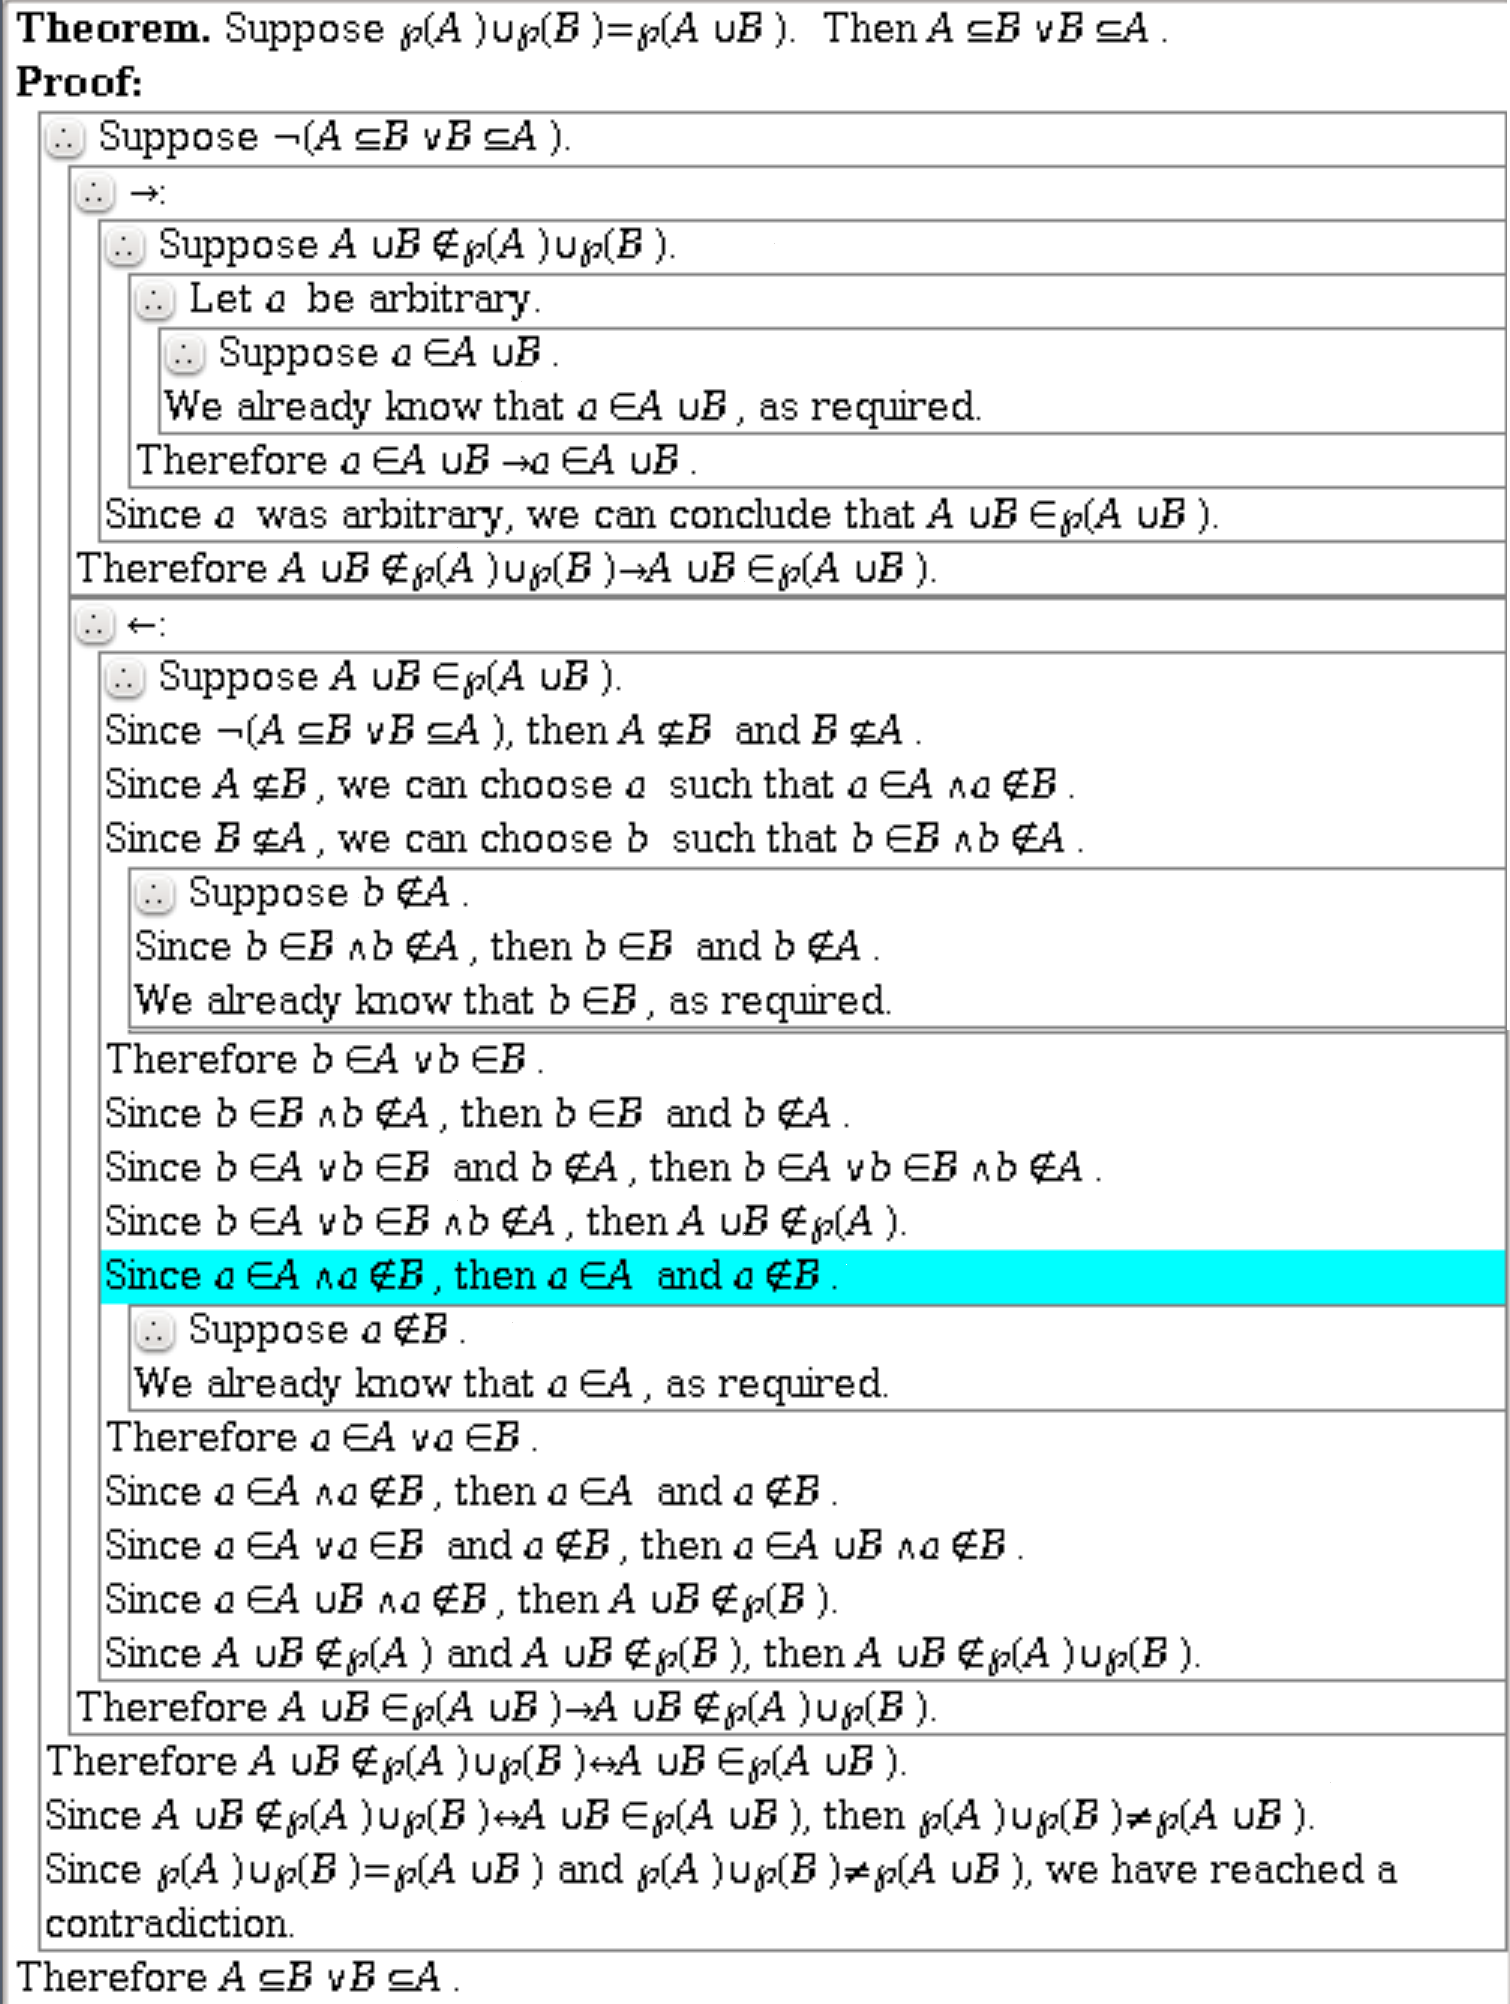
\includegraphics[scale=0.15]{3_5_8}

\vspace{30pt}

9. Suppose x and y are real numbers and $x \neq 0$. Prove that $y + 1/x =
1 + y/x$ iff either $x = 1$ or $y = 1$.

\vspace{30pt}


\centerline{
  \begin{tabular}{l l}
  \textit{Givens} & \textit{Goal} \\
    $x \neq 0$ & $y + 1/x = 1 + y/x \leftrightarrow (x = 1 \text{ or } y = 1)$ \\
  \end{tabular}}
\vspace{20pt}

\centerline{($\rightarrow$)}

\centerline{
  \begin{tabular}{l l}
  \textit{Givens} & \textit{Goal} \\
    $x \neq 0$ & $x = 1 \text{ or } y = 1$ \\
    $y + 1/x = 1 + y/x$ & \\
  \end{tabular}}
\vspace{20pt}

$y + 1/x = 1 + y/x$

$xy + 1 = x + y$

$x(y - 1) = y - 1$

$x = \frac{y - 1}{y - 1}$

$x = 1$

\centerline{($\leftarrow$)}

\centerline{
  \begin{tabular}{l l}
  \textit{Givens} & \textit{Goal} \\
    $x \neq 0$ & $y + 1/x = 1 + y/x$ \\
    $x = 1 \text{ or } y = 1$ & \\
  \end{tabular}}
\vspace{20pt}

Case 1

\centerline{
  \begin{tabular}{l l}
  \textit{Givens} & \textit{Goal} \\
    $x \neq 0$ & $y + 1/x = 1 + y/x$ \\
    $x = 1$ & \\
  \end{tabular}}
\vspace{20pt}

$y + 1/x = 1 + y/x$

$y + 1 = 1 + y$

\vspace{20pt}

Case 2

\centerline{
  \begin{tabular}{l l}
  \textit{Givens} & \textit{Goal} \\
    $x \neq 0$ & $y + 1/x = 1 + y/x$ \\
    $y = 1$ & \\
  \end{tabular}}
\vspace{20pt}

$y + 1/x = 1 + y/x$

$1 + 1/x = 1 + 1/x$

\vspace{20pt}

\textbf{Theorem.} x and y are real numbers and $x \neq 0$. If $y + 1/x =
1 + y/x$ iff either $x = 1$ or $y = 1$.

\textit{Proof.} Suppose $y + 1/x = 1 + y/x$. Then.

$y + 1/x = 1 + y/x$

$\frac{xy + 1}{x} = \frac{x + y}{x}$

Since $x \neq 0$

$xy + 1 = x + y$

$x(y - 1) = y - 1$

$x = \frac{y - 1}{y - 1}$

Since $y = 1$

$x = 1$

Therefore, $x = 1$.

Now suppose $x = 1$ or $y = 1$.

Case 1. $x = 1$. Then

$y + 1/1 = 1 + y/1$

$y + 1 = y + 1$

Case 2. $y = 1$. Then

$y + 1/x = 1 + y/x$

$1 + 1/x = 1 + 1/x$

Therefore $y + 1/x = 1 + y/x$.

Thus, if $y + 1/x = 1 + y/x$ iff either $x = 1$ or $y = 1$.

\vspace{30pt}

10. Prove that for every real number x, if $|x - 3| > 3$ then $x^2 > 6x$. (Hint:
According to the definition of $|x - 3|$, if $x - 3 \geq 0$ then $|x - 3| = x - 3$, and if $x - 3 < 0$ then $|x - 3| = 3 - x$. The easiest way to use this fact is to break your proof into cases. Assume that $x - 3 \geq 0$ in case 1, and $x - 3 < 0$ in case 2.)
\vspace{30pt}

Let x be an arbitrary real number.

Case 1. $x - 3 \geq 0$

Then $|x - 3| = x - 3$. Suppose $|x - 3| > 3$. Then $x - 3 > 3$

$x > 6$

$x * x > 6 x$

$x^2 > 6x$

Thus, $x^2 > 6x$.


Case 2. $x - 3 < 0$

Then $|x - 3| = 3 - x$. Suppose $|x - 3| > 3$. Then $3 - x > 3$

$3 - x > 3$

$-3 + x < -3$

$x < 0$

Since $x < 0$, then $x^2 > 6x$.    

Since x was arbitrary $\forall x \in \mathbb{R}(|x - 3| > 3 \to x^2 > 6x)$


\vspace{30pt}

*11. Prove that for every real number x, $|2x - 6| > x$ iff $|x - 4| > 2$. (Hint: Read the hint for exercise 10.)

\vspace{30pt}

\centerline{
  \begin{tabular}{l l}
  \textit{Givens} & \textit{Goal} \\
    $|2x - 6| > x$ & $|x - 4| > 2$ \\
  \end{tabular}}
\vspace{20pt}

\centerline{
  \begin{tabular}{l l}
  \textit{Givens} & \textit{Goal} \\
    $|2x - 6| > x$ & $|x - 4| > 2$ \\
  \end{tabular}}
\vspace{20pt}

Case 1. $2x - 6 \geq 0$.

$2x - 6 > x$

$x > 6$

$x - 4 > 6 - 4$

Since $x - 4 > 2$ is positive.

Thus, $x - 4 > 2$.

Case 2. $2x - 6 < 0$

$6 - 2x > x$

$3x < 6$

$x < 2$.

$-x > -2$

$4 - x > 2$

$x < 2$

$x - 4 < - 2$ is negative.

Thus, $4 - x > 2$.

\centerline{
  \begin{tabular}{l l}
  \textit{Givens} & \textit{Goal} \\
    $|x - 4| > 2$ & $|2x - 6| > x$ \\
  \end{tabular}}
\vspace{20pt}

Case 1. $x - 4 \geq 0$

$x - 4 > 2$

$x > 6$

$2x > 6 + x$

$2x - 6 > x$

Since $x > 6$, $2x - 6$ is positive, thus $2x - 6 > x$

Case 2. $x - 4 < 0$

$4 - x > 2$

$x < 2$

$3x < 6$

$x < 6 - 2x$

$2x < 4$

Since $2x - 6 < - 2$, $2x - 6 < -2$ is negative. 

Thus, $6 - 2x > x$

\textbf{Theorem.} For every real number x, $|2x - 6| > x$ iff $|x - 4| > 2$.

\textit{Proof.} Let x be an arbitrary real number.

Suppose $|2x - 6| > x$.

Case 1. $2x - 6 \geq 0$

$x > 6$

$x - 4 > 2$

Since $x - 4 > 2$ is positive.

Thus, $|x - 4| = x - 4 > 2$

Case 2. $2x - 6 < 0$

$x < 2$

$4 - x > 2$

Since $x - 4 < -2$ is negative

Thus, $|x - 4| = 4 - x > 2$

Now suppose $|x - 4| > 2$.

Case 1. $x - 4 \geq 0$

$x > 6$

Since $2x - 6 > x$ is positive.

Thus, $2x - 6 > x$

Case 2. $x - 4 < 0$

$x < 2$

$6 - 2x > x$

Since $2x - 6 < -2$ is negative.

Thus, $6 - 2x > x$

Since x was an arbitrary real number, $\forall x \in \mathbb{R}(|2x - 6| > x \leftrightarrow |x - 4| > 2)$

\vspace{30pt}

12. (a) Prove that for all real numbers a and b, $|a| \leq b$ iff $-b \leq a \leq b$.

\hspace{12pt}(b) Prove that for any real number x, $-|x| \leq x \leq |x|$. (Hint: Use part (a).)

\hspace{12pt}(c) Prove that for all real numbers x and y, $|x + y| \leq |x| + |y|$. (This is called the triangle inequality. One way to prove this is to combine parts (a) and (b), but you can also do it by considering a number of
cases.)

\vspace{30pt}

(a)

\centerline{
  \begin{tabular}{l l}
  \textit{Givens} & \textit{Goal} \\
    $|a| \leq b$ & $a \leq b \land a \geq -b$ \\
  \end{tabular}}
\vspace{20pt}

Case 1. $a \geq 0$

$a \leq b$.

Since $a \geq 0$ and $a \leq b$, it follows that $a \geq -b$.

Thus, $a \leq b \land a \geq -b$.

Case 2. $a < 0$

$-a \leq b$

$a \geq -b$

Since $a \geq -b$ and $a < 0$, it follows that $a \leq b$. 

Thus, $a \leq b \land a \geq -b$.

\centerline{
  \begin{tabular}{l l}
  \textit{Givens} & \textit{Goal} \\
    $-b \leq a \leq b$ & $|a| \leq b$ \\
  \end{tabular}}
\vspace{20pt}

\centerline{
  \begin{tabular}{l l}
  \textit{Givens} & \textit{Goal} \\
    $a \leq b$ & $|a| \leq b$ \\
    $a \geq -b$ & \\
  \end{tabular}}
\vspace{20pt}

Case 1. $a \geq 0$

Thus, $a \leq b$

Case 2. $a < 0$

$-a \leq b$

Thus, $a \geq -b$.

\vspace{30pt}

\textbf{Theorem.} For all real numbers a and b, $|a| \leq b$ iff $-b \leq a \leq b$.

\textit{Proof.} Let a, b be arbitrary real numbers.

Suppose $|a| \leq b$.

Case 1. $a \geq 0$

$a \leq b$

Since $a \geq 0$ and $a \leq b$, it follows that $a \geq -b$

Thus $-b \leq a \leq b$

Case 2. $a < 0$

$-a \leq b$

$a \geq -b$

Since $a \geq -b$ and $a < 0$, it follows that $a \leq b$

Thus, $-b \leq a \leq b$.

Now suppose $-b \leq a \leq b$.

Case 1. $a \geq 0$

Thus $a \leq b$.

Case 2. $a < 0$

$-a \leq b$

Thus, $a \geq -b$

Therefore, $\forall a \in \mathbb{R} b \in \mathbb{R} (|a| \leq b \leftrightarrow -b \leq a \leq b$).

\vspace{30pt}

(b)

\centerline{
  \begin{tabular}{l l}
  \textit{Givens} & \textit{Goal} \\
    $|a| \leq b = -b \leq a \leq b$ & $-|x| \leq x \leq |x|$ \\
  \end{tabular}}
\vspace{10pt}

$|x| \leq |x|$

\textbf{Theorem.} For any real number x, $-|x| \leq x \leq |x|$.

Suppose $|a| \leq b$ is equivalent to $-b \leq a \leq b$ (using results from (a)). Then

$-|x| \leq x \leq |x|$ is $|x| \leq |x|$ which is always true.

Thus, $-|x| \leq x \leq |x|$.

\vspace{30pt}

(c) Prove that for all real numbers x and y, $|x + y| \leq |x| + |y|$. (This is called the triangle inequality. One way to prove this is to combine parts (a) and (b), but you can also do it by considering a number of
cases.)

\centerline{
  \begin{tabular}{l l}
  \textit{Givens} & \textit{Goal} \\
    $$ & $|x + y| \leq |x| + |y|$ \\
  \end{tabular}}
\vspace{10pt}

\textbf{Theorem.} For all real numbers x and y, $|x + y| \leq |x| + |y|$.

Using theorem from (b)

$-|x| \leq x \leq |x|$

$-|y| \leq y \leq |y|$

Let's add them:

$-(|x|+|y|) \leq x + y \leq |x|+|y|$

Using theorem from (a)

$|x + y| \leq |x| + |y|$

\vspace{30pt}

13. Prove that for every integer x, $x^2 + x$ is even.

\vspace{30pt}

\centerline{
  \begin{tabular}{l l}
  \textit{Givens} & \textit{Goal} \\
    $$ & $x^2 + x$ \\
  \end{tabular}}
\vspace{10pt}

$x = 1$, $1 + 1 = 2$

$x = 2$, $4 + 2 = 6$

$x = 3$, $9 + 3 = 12$

$x = 4$, $16 + 4 = 20$

Case 1. x is odd.

$\exists k (2k + 1 = x)$

$2k + 1 = x$

$(2k + 1)^2 + (2k + 1) = (4k^2 + 4k + 1) + (2k + 1) = 4k^2 + 6k + 2 = 2(2k^2 + 3k + 1)$

Case 2. x is even.

$\exists m (2m = x)$

$4m^2 + 2m = 2(2m^2 + m)$
\vspace{20pt}

\textit{Proof.} Let x be an arbitrary integer.

Case 1. x is odd.

Then we can choose some $k \in \mathbb{Z}$ such that $2k + 1 = x$.

$(2k + 1)^2 + (2k + 1) = 4k^2 + 6k + 2 = 2(2k^2 + 3k + 1)$

Thus, $x^2 + x$ is even.

Case 2. x is even.

Then we can choose some $m \in \mathbb{Z}$ such that $2m = x$

$4m^2 + 2m = 2(2m^2 + m)$

Thus, $x^2 + x$ is even.

Since x was an arbitrary integer we can conclude that $\forall x \in \mathbb{Z} (x^2 + x \text{ is even})$.

\vspace{30pt}

14. Prove that for every integer x, the remainder when $x^4$ is divided by 8 is either 0 or 1.

\vspace{30pt}

Case 1. x is odd

$\exists k (2k + 1 = x)$

$\frac{(2k + 1)^4}{8}$

$(2k+1)^4 = 16k^4 + 32k^3 + 24k^2 + 8k + 1 = 2(8k^4 + 16k^3 + 12k^2 + 4k) + 1$

Case 2. x is even

$\exists m (2m = x)$

$\frac{16k^4}{8} = 2k^4$
\vspace{20pt}

\textbf{Theorem.} For every integer x, the remainder when $x^4$ is divided by 8 is either 0 or 1.

\textit{Proof.} Let x be an arbitrary integer.

Case 1. x is odd. Then we can choose some $k \in \mathbb{Z}$ such that $2k + 1 = x$

$(2k+1)^4 = 16k^4 + 32k^3 + 24k^2 + 8k + 1 = 2(8k^4 + 16k^3 + 12k^2 + 4k) + 1$

Thus, the remainder when $x^4$ is divided by 8 is always 1 if x is odd.

Case 2. x is even. Then we can choose some $m \in \mathbb{Z}$ such that $2m = x$

$\frac{16k^4}{8} = 2k^4$

Thus, the remainder when $x^4$ is divided by 8 is always 0 if x is even.

Since x was an arbitrary integer, for every integer x, the remainder when $x^4$ is divided by 8 is either 0 or 1.

\vspace{30pt}

*15. Suppose $\mathcal{F}$ and $\mathcal{G}$ are nonempty families of sets.

\hspace{12pt}$^{\textit{P}}_{\, \textit{D}}$ (a) Prove that $\cup(\mathcal{F} \cup \mathcal{G}) = (\cup\mathcal{F}) \cup (\cup\mathcal{G})$.

\hspace{12pt}(b) Can you discover and prove a similar theorem about $\cap(\mathcal{F} \cup \mathcal{G})$?

\vspace{30pt}

(a)

\textbf{3.5.15.pd}
\vspace{10pt}

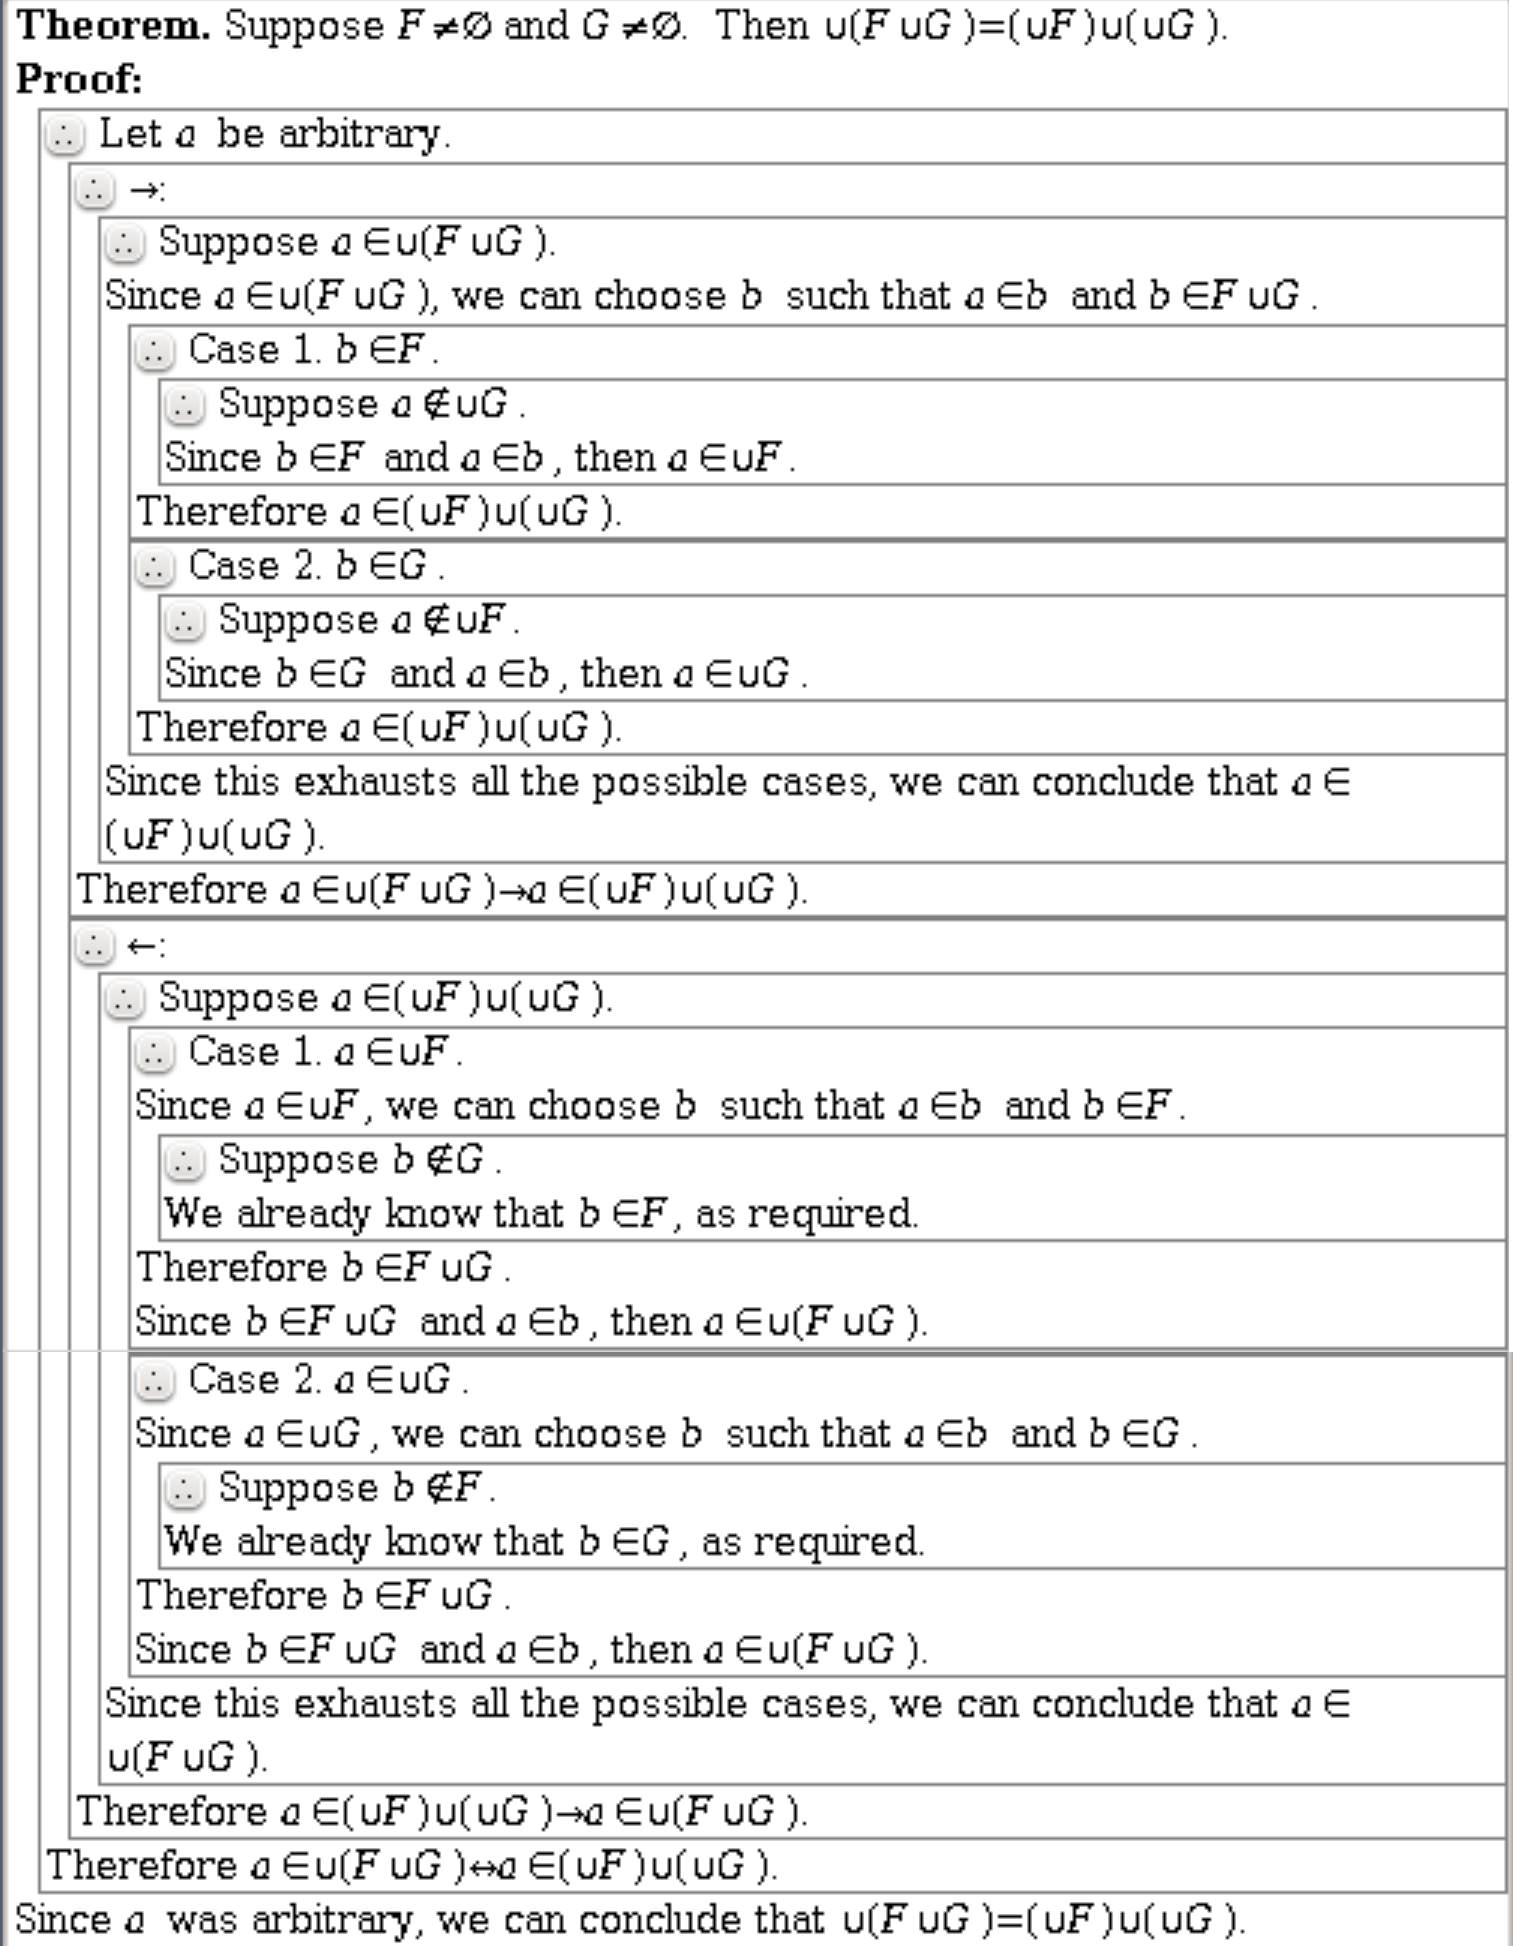
\includegraphics[scale=0.15]{3_5_15}

\vspace{30pt}

(b)

\centerline{
  \begin{tabular}{l l}
  \textit{Givens} & \textit{Goal} \\
    $$ & $\cap(\mathcal{F} \cup \mathcal{G}) = ??$ \\
  \end{tabular}}
\vspace{10pt}

$\forall A (A \in (\mathcal{F} \cup \mathcal{G}) \to x \in A)$

$\forall A ((A \notin \mathcal{F} \land A \notin \mathcal{G}) \lor x \in A)$

$\forall A [(A \notin \mathcal{F} \lor x \in A) \land (A \notin \mathcal{G} \lor x \in A)]$

$\forall A [(A \in \mathcal{F} \to x \in A) \land (A \in \mathcal{G} \to x \in A)]$

$\forall A (A \in \mathcal{F} \to x \in A) \land \forall A (A \in \mathcal{G} \to x \in A)]$

$(\cap \mathcal{F}) \cap (\cap \mathcal{G})$

\centerline{
  \begin{tabular}{l l}
  \textit{Givens} & \textit{Goal} \\
    $(\cap \mathcal{F}) \cap (\cap \mathcal{G})$ & $\cap(\mathcal{F} \cup \mathcal{G})$ \\
  \end{tabular}}
\vspace{10pt}

\centerline{
  \begin{tabular}{l l}
  \textit{Givens} & \textit{Goal} \\
    $(\cap \mathcal{F}) \cap (\cap \mathcal{G})$ & $\forall A [A \in (\mathcal{F} \cup \mathcal{G}) \to x \in A]$ \\
  \end{tabular}}
\vspace{10pt}

\centerline{
  \begin{tabular}{l l}
  \textit{Givens} & \textit{Goal} \\
    $(\cap \mathcal{F}) \cap (\cap \mathcal{G})$ & $x \in A$ \\
    $A \in (\mathcal{F} \cup \mathcal{G})$ & \\
  \end{tabular}}
\vspace{10pt}

\centerline{
  \begin{tabular}{l l}
  \textit{Givens} & \textit{Goal} \\
    $(\cap \mathcal{F}) \cap (\cap \mathcal{G})$ & $x \in A$ \\
    $A \in \mathcal{F} \lor A \in \mathcal{G}$ & \\
  \end{tabular}}
\vspace{10pt}

\centerline{
  \begin{tabular}{l l}
  \textit{Givens} & \textit{Goal} \\
    $\forall A (A \in \mathcal{F} \to x \in A)$ & $x \in A$ \\
    $\forall A (A \in \mathcal{G} \to x \in A)$ & \\
    $A \in \mathcal{F} \lor A \in \mathcal{G}$ & \\
  \end{tabular}}
\vspace{10pt}

\vspace{20pt}

\centerline{
  \begin{tabular}{l l}
  \textit{Givens} & \textit{Goal} \\
    $\cap (\mathcal{F} \cup \mathcal{G})$ & $(\cap \mathcal{F}) \cap (\cap \mathcal{G})$ \\
 \end{tabular}}
\vspace{10pt}

\centerline{
  \begin{tabular}{l l}
  \textit{Givens} & \textit{Goal} \\
    $\cap (\mathcal{F} \cup \mathcal{G})$ & $\forall A (A \in \mathcal{F} \to x \in A)$ \\
 \end{tabular}}
\vspace{30pt}

\centerline{
  \begin{tabular}{l l}
  \textit{Givens} & \textit{Goal} \\
    $\cap (\mathcal{F} \cup \mathcal{G})$ & $x \in A$ \\
    $A \in \mathcal{F}$ & \\
 \end{tabular}}
\vspace{30pt}

\centerline{
  \begin{tabular}{l l}
  \textit{Givens} & \textit{Goal} \\
    $\forall A (A \in \mathcal{F} \cup \mathcal{G} \to x \in A)$ & $x \in A$ \\
    $A \in \mathcal{F}$ & \\
 \end{tabular}}
\vspace{30pt}

\vspace{20pt}

\centerline{
  \begin{tabular}{l l}
  \textit{Givens} & \textit{Goal} \\
    $\forall A (A \in \mathcal{F} \cup \mathcal{G} \to x \in A)$ & $x \in A$ \\
    $A \in \mathcal{G}$ & \\
 \end{tabular}}
\vspace{10pt}

\textbf{Theorem.} $\cap(\mathcal{F} \cup \mathcal{G}) = (\cap \mathcal{F}) \cap (\cap \mathcal{G})$ 

\textit{Proof.} Let B be an arbitrary.

Suppose $(\cap \mathcal{F}) \cap (\cap \mathcal{G})$.
Let A be an arbitrary.
Suppose $A \in (\mathcal{F} \cup \mathcal{G})$.
Since $A \in \mathcal{F} \lor A \in \mathcal{G}$ and $\cap \mathcal{F}$, $x \in A$
Since $A \in \mathcal{F} \lor A \in \mathcal{G}$ and $\cap \mathcal{G}$, $x \in A$
Therefore, $x \in A$
Therefore, $\cap (\mathcal{F} \cup \mathcal{G})$.
\vspace{10pt}

Suppose $\cap (\mathcal{F} \cup \mathcal{G})$.

Let A be an arbitrary.
Suppose $A \in F$.
Since $A \in F$ and $\cap (\mathcal{F} \cup \mathcal{G})$, $x \in A$.
Therefore, $\cap \mathcal{F}$.

Let A be an arbitrary.
Suppose $A \in G$
Since $A \in G$ and $\cap (\mathcal{F} \cup \mathcal{G})$, $x \in A$.
Therefore, $\cap \mathcal{G}$.

Thus, $(\cap \mathcal{F}) \cap (\cap \mathcal{G})$.
\vspace{10pt}

Since B was an arbitrary, $\cap(\mathcal{F} \cup \mathcal{G}) = (\cap \mathcal{F}) \cap (\cap \mathcal{G})$.


\vspace{30pt}

16. Suppose $\mathcal{F}$ is a nonempty family of sets and B is a set.

\hspace{12pt}$^{\textit{P}}_{\, \textit{D}}$ (a) Prove that $B \cup (\cup\mathcal{F}) = \cup(\mathcal{F} \cup {B})$.

\hspace{12pt}(b) Prove that $B \cup (\cap\mathcal{F}) = \cap_{A \in \mathcal{F}} (B \cup A)$.

\hspace{12pt}(c) Can you discover and prove a similar theorem about $B \cap (\cap \mathcal{F} )$?

\vspace{30pt}

(a)

\textbf{3.5.16.pd}
\vspace{10pt}

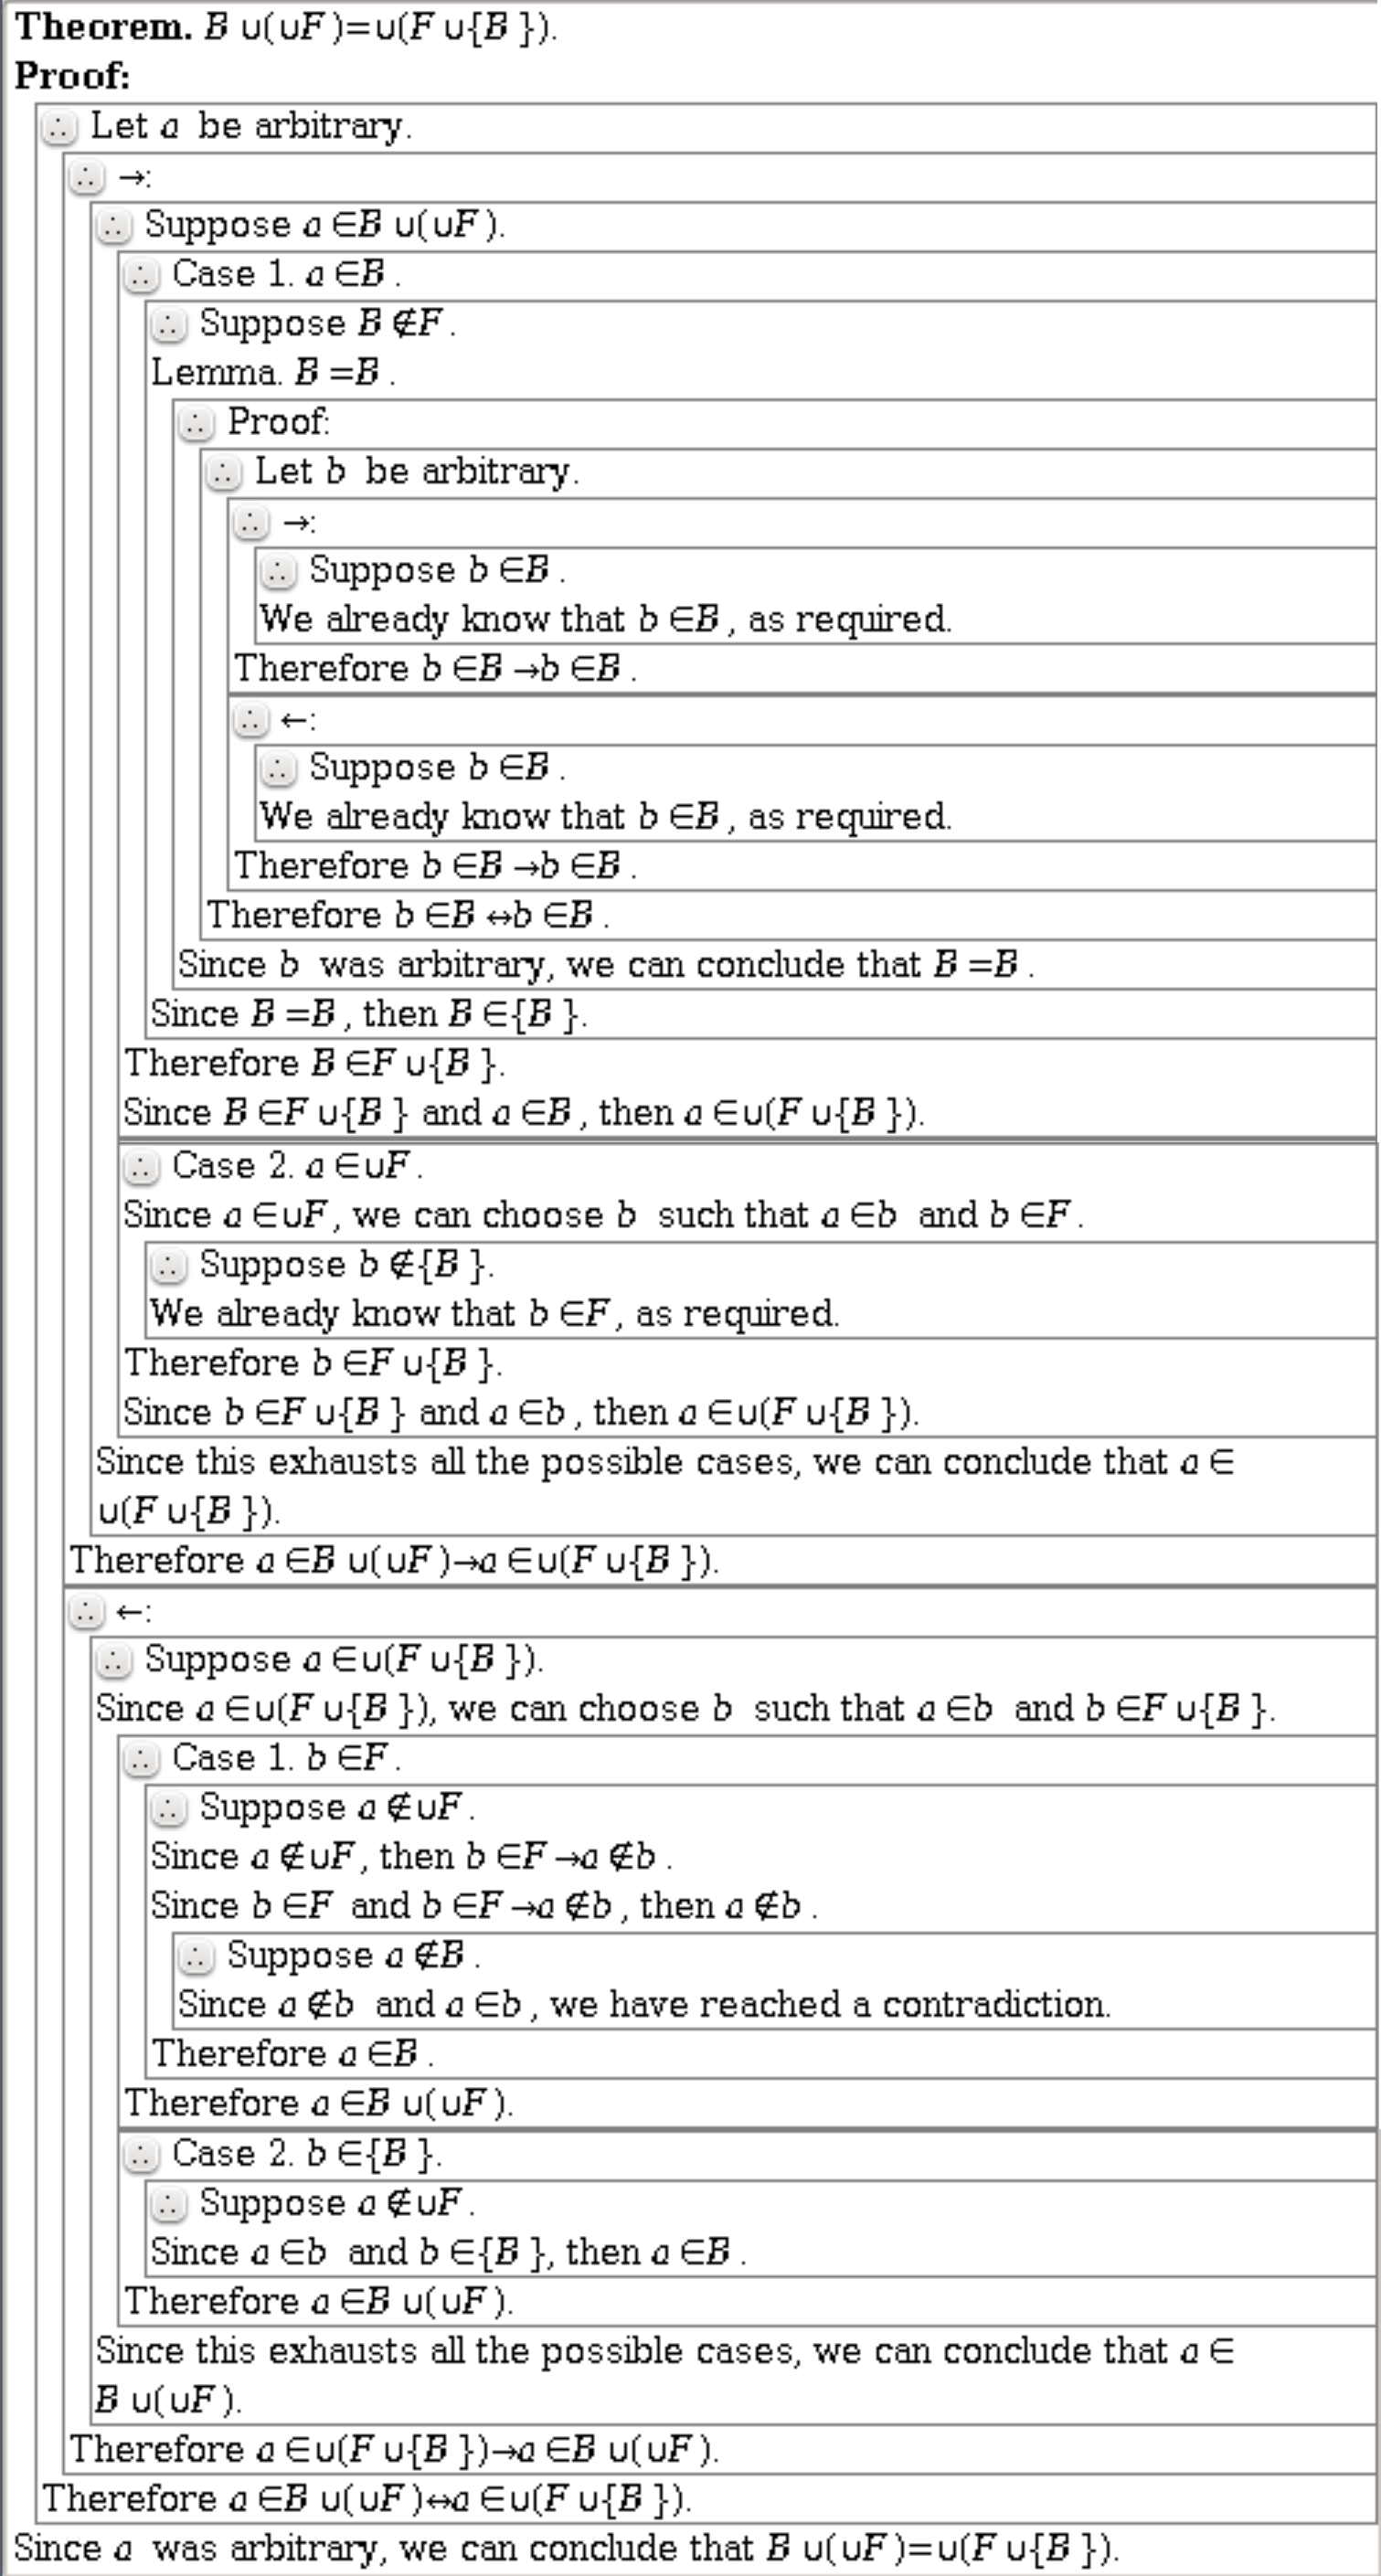
\includegraphics[scale=0.15]{3_5_16}

\vspace{30pt}

(b)

\centerline{
  \begin{tabular}{l l}
  \textit{Givens} & \textit{Goal} \\
    $$ & $B \cup (\cap\mathcal{F}) = \cap_{A \in \mathcal{F}} (B \cup A)$ \\
 \end{tabular}}
\vspace{10pt}

$\rightarrow$

\centerline{
  \begin{tabular}{l l}
  \textit{Givens} & \textit{Goal} \\
    $B \cup (\cap\mathcal{F})$ & $\cap_{A \in \mathcal{F}} (B \cup A)$ \\
 \end{tabular}}
\vspace{10pt}

$\cap_{A \in \mathcal{F}} (B \cup A)$

$\forall A \in \mathcal{F} (x \in (B \cup A))$

$\forall A [A \in \mathcal{F} \to (x \in (B \cup A)]$

\centerline{
  \begin{tabular}{l l}
  \textit{Givens} & \textit{Goal} \\
    $x \in B \lor x \in (\cap\mathcal{F})$ & $x \in B \lor x \in A$ \\
    $A \in \mathcal{F}$ & \\
 \end{tabular}}
\vspace{10pt}

$x \in (\cap\mathcal{F})$

$\forall A (A \in \mathcal{F} \to x \in A)$


\centerline{
  \begin{tabular}{l l}
  \textit{Givens} & \textit{Goal} \\
    $x \in B \lor x \in A$ & $x \in B \lor x \in A$ \\
 \end{tabular}}
\vspace{10pt}

$\leftarrow$

\centerline{
  \begin{tabular}{l l}
  \textit{Givens} & \textit{Goal} \\
    $\cap_{A \in \mathcal{F}} (B \cup A)$ & $B \cup (\cap\mathcal{F})$ \\
 \end{tabular}}
\vspace{10pt}

\centerline{
  \begin{tabular}{l l}
  \textit{Givens} & \textit{Goal} \\
    $\cap_{A \in \mathcal{F}} (B \cup A)$ & $x \in B \lor x \in (\cap \mathcal{F})$ \\
 \end{tabular}}
\vspace{10pt}

\centerline{
  \begin{tabular}{l l}
  \textit{Givens} & \textit{Goal} \\
    $\forall A \in \mathcal{F}(x \in (B \cup A))$ & $x \in B \lor x \in (\cap \mathcal{F})$ \\
 \end{tabular}}
\vspace{10pt}

\centerline{
  \begin{tabular}{l l}
  \textit{Givens} & \textit{Goal} \\
    $\forall A [A \in \mathcal{F} \to x \in B \lor x \in A]$ & $x \in B \lor x \in (\cap \mathcal{F})$ \\
 \end{tabular}}
\vspace{10pt}

\centerline{
  \begin{tabular}{l l}
  \textit{Givens} & \textit{Goal} \\
    $\forall A [A \in \mathcal{F} \to x \in B \lor x \in A]$ & $x \in (\cap \mathcal{F})$ \\
    $x \notin B$
 \end{tabular}}
\vspace{10pt}

\centerline{
  \begin{tabular}{l l}
  \textit{Givens} & \textit{Goal} \\
    $\forall A [A \in \mathcal{F} \to x \in B \lor x \in A]$ & $\forall A (A \in \mathcal{F} \to x \in A)$ \\
    $x \notin B$
 \end{tabular}}
\vspace{10pt}

\centerline{
  \begin{tabular}{l l}
  \textit{Givens} & \textit{Goal} \\
    $\forall A [A \in \mathcal{F} \to x \in B \lor x \in A]$ & $x \in A$ \\
    $x \notin B$ & \\
    $A \in \mathcal{F}$ & \\
 \end{tabular}}
\vspace{10pt}

\centerline{
  \begin{tabular}{l l}
  \textit{Givens} & \textit{Goal} \\
    $x \in B \lor x \in A$ & $x \in A$ \\
    $x \notin B$ & \\
    $A \in \mathcal{F}$ & \\
 \end{tabular}}
\vspace{10pt}

\textbf{Theorem.} $B \cup (\cap\mathcal{F}) = \cap_{A \in \mathcal{F}} (B \cup A)$

\textit{Proof.} Suppose $B \cup (\cap\mathcal{F})$. 
Then $x \in B$ or $x \in (\cap \mathcal{F})$. 
Let A be an arbitrary element.
Suppose $A \in \mathcal{F}$.
Since $x \in (\cap\mathcal{F})$ and $A \in \mathcal{F}$, $x \in A$.
Therefore, $x \in B$ or $x \in A$.
Since A was arbitrary, we can conclude $\cap_{A \in \mathcal{F}} (B \cup A)$.

Now suppose $\cap_{A \in \mathcal{F}} (B \cup A)$.
Suppose, $x \notin B$.
Let C be an arbitrary element.
Suppose $C \in \mathcal{F}$.
Since $\cap_{A \in \mathcal{F}} (B \cup A)$ and $C \in \mathcal{F}$, $x \in B$ or $x \in C$.
Since $x \in B$ or $x \in C$ and $x \notin B$, $x \in C$.
Therefore, $x \in C$
Thus, $x \in (\cap \mathcal{F})$.
Therefore, $B \cup (\cap\mathcal{F})$.

Thus, $B \cup (\cap\mathcal{F}) = \cap_{A \in \mathcal{F}} (B \cup A)$

\vspace{30pt}

(c) $B \cap (\cap \mathcal{F}) = \cap_{x \in B \to A \in \mathcal{F}} (A \cap B)$

$\rightarrow$

\centerline{
  \begin{tabular}{l l}
  \textit{Givens} & \textit{Goal} \\
    $B \cap (\cap \mathcal{F})$ & $\cap_{x \in B \to A \in \mathcal{F}} (A \cap B)$ \\
 \end{tabular}}
\vspace{10pt}

\centerline{
  \begin{tabular}{l l}
  \textit{Givens} & \textit{Goal} \\
    $B \cap (\cap \mathcal{F})$ & $\forall A ((x \in B \to A \in \mathcal{F}) \to A \cap B)$ \\
 \end{tabular}}
\vspace{10pt}

\centerline{
  \begin{tabular}{l l}
  \textit{Givens} & \textit{Goal} \\
    $\forall A (A \in \mathcal{F} \to x \in A)$ & $A \cap B$ \\
    $x \in B \to A \in \mathcal{F}$ & \\
    $x \in B$
 \end{tabular}}
\vspace{10pt}

\centerline{
  \begin{tabular}{l l}
  \textit{Givens} & \textit{Goal} \\
    $\forall A (A \in \mathcal{F} \to x \in A)$ & $A \cap B$ \\
    $x \in B$ & \\
    $A \in \mathcal{F}$ & \\
 \end{tabular}}
\vspace{10pt}

\centerline{
  \begin{tabular}{l l}
  \textit{Givens} & \textit{Goal} \\
    $x \in A$ & $A \cap B$ \\
    $x \in B$ & \\
    $A \in \mathcal{F}$ & \\
 \end{tabular}}
\vspace{10pt}

$\leftarrow$

\centerline{
  \begin{tabular}{l l}
  \textit{Givens} & \textit{Goal} \\
    $\cap_{x \in B \to A \in \mathcal{F}} (A \cap B)$ & $B \cap (\cap \mathcal{F})$ \\
 \end{tabular}}
\vspace{10pt}

$B \cap (\cap \mathcal{F})$

$\forall A (A \in \mathcal{F} \to x \in A)$

$\forall A (x \in B \land (A \notin \mathcal{F} \lor x \in A))$

$\forall A ((x \in B \land A \notin \mathcal{F}) \lor (x \in B \land x \in A)$

\centerline{
  \begin{tabular}{l l}
  \textit{Givens} & \textit{Goal} \\
    $\forall A ((x \in B \to A \in \mathcal{F}) \to (x \in A \land x \in B))$ & $\forall A ((x \in B \land A \notin \mathcal{F}) \lor (x \in B \land x \in A))$ \\
 \end{tabular}}
\vspace{10pt}

\centerline{
  \begin{tabular}{l l}
  \textit{Givens} & \textit{Goal} \\
    $\forall A ((x \in B \to A \in \mathcal{F}) \to (x \in A \land x \in B))$ & $x \in B \land x \in A$ \\
    $x \in B \to A \in \mathcal{F}$
 \end{tabular}}
\vspace{10pt}

\textbf{Theorem.} $B \cap (\cap \mathcal{F}) = \cap_{x \in B \to A \in \mathcal{F}} (A \cap B)$

\textit{Proof.} Suppose $B \cap (\cap \mathcal{F})$.
Then $x \in B$ and $x \in \cap \mathcal{F}$.
Let A be arbitrary element.
Suppose $x \in B \to A \in \mathcal{F}$
Since $x \in B$ and $x \in B \to A \in \mathcal{F}$, $A \in \mathcal{F}$
Since $x \in \cap \mathcal{F}$ and $A \in \mathcal{F}$, $x \in A$
Since $x \in A$ and $x \in B$, $x \in A \cap B$
Thus, $A \cap B$.
Since A was arbitrary, we can conclude that $\cap_{x \in B \to A \in \mathcal{F}} (A \cap B)$.
\vspace{10pt}

Now suppose, $\cap_{x \in B \to A \in \mathcal{F}} (A \cap B)$.

$B \cap (\cap \mathcal{F})$ is equivalent to

$\forall A (A \in \mathcal{F} \to x \in A)$ is equivalent to

$\forall A (x \in B \land (A \notin \mathcal{F} \lor x \in A))$ is equivalent to

$\forall A ((x \in B \land A \notin \mathcal{F}) \lor (x \in B \land x \in A)$

Let A be arbitrary.
Suppose, $x \in B \to A \in \mathcal{F}$
Since $x \in B \to A \in \mathcal{F}$ and $\cap_{x \in B \to A \in \mathcal{F}} (A \cap B)$, $x \in B \land x \in A$
Thus, $x \in B \land x \in A$
Thus, $B \cap (\cap \mathcal{F})$
\vspace{10pt}

Therefore, $B \cap (\cap \mathcal{F}) = \cap_{x \in B \to A \in \mathcal{F}} (A \cap B)$

\vspace{30pt}

17. Suppose $\mathcal{F}$, $\mathcal{G}$, and $\mathcal{H}$ are nonempty families of sets and for every $A \in \mathcal{F}$ and every $B \in \mathcal{G}$, $A \cup B \in \mathcal{H}$. Prove that $\cap\mathcal{H} \subseteq (\cap\mathcal{F}) \cup (\cap\mathcal{G})$.

\vspace{30pt}

\centerline{
  \begin{tabular}{l l}
  \textit{Givens} & \textit{Goal} \\
    $\forall A \in \mathcal{F} \forall B \in \mathcal{G} (A \cup B \in \mathcal{H})$ & $\cap\mathcal{H} \subseteq (\cap\mathcal{F}) \cup (\cap\mathcal{G})$ \\
 \end{tabular}}
\vspace{10pt}

$\cap\mathcal{H} \subseteq (\cap\mathcal{F}) \cup (\cap\mathcal{G})$

$\forall C (C \in \cap \mathcal{H} \to C \in (\cap\mathcal{F}) \cup (\cap\mathcal{G}))$

\centerline{
  \begin{tabular}{l l}
  \textit{Givens} & \textit{Goal} \\
    $\forall A \in \mathcal{F} \forall B \in \mathcal{G} (A \cup B \in \mathcal{H})$ & $C \in \cap \mathcal{H} \to C \in (\cap\mathcal{F}) \cup (\cap\mathcal{G})$ \\
 \end{tabular}}
\vspace{10pt}

\centerline{
  \begin{tabular}{l l}
  \textit{Givens} & \textit{Goal} \\
    $\forall A \in \mathcal{F} \forall B \in \mathcal{G} (A \cup B \in \mathcal{H})$ & $C \in (\cap\mathcal{F}) \cup (\cap\mathcal{G})$ \\
    $C \in \cap \mathcal{H}$ & \\
 \end{tabular}}
\vspace{10pt}

\centerline{
  \begin{tabular}{l l}
  \textit{Givens} & \textit{Goal} \\
    $\forall A \in \mathcal{F} \forall B \in \mathcal{G} (A \cup B \in \mathcal{H})$ & $C \in \cap\mathcal{F} \lor C \in \cap\mathcal{G}$ \\
    $C \in \cap \mathcal{H}$ & \\
 \end{tabular}}
\vspace{10pt}

\centerline{
  \begin{tabular}{l l}
  \textit{Givens} & \textit{Goal} \\
    $\forall A \in \mathcal{F} \forall B \in \mathcal{G} (A \cup B \in \mathcal{H})$ & $C \in \cap\mathcal{F}$ \\
    $\forall T (T \in \mathcal{H} \to C \in T)$ & \\
    $C \notin \cap\mathcal{G}$ & \\
 \end{tabular}}
\vspace{10pt}

\centerline{
  \begin{tabular}{l l}
  \textit{Givens} & \textit{Goal} \\
    $\forall A \in \mathcal{F} \forall B \in \mathcal{G} (A \cup B \in \mathcal{H})$ & $\forall T (T \in \mathcal{F} \to C \in T)$ \\
    $\forall T (T \in \mathcal{H} \to C \in T)$ & \\
    $C \notin \cap\mathcal{G}$ & \\
 \end{tabular}}
\vspace{10pt}

\centerline{
  \begin{tabular}{l l}
  \textit{Givens} & \textit{Goal} \\
    $\forall A \in \mathcal{F} \forall B \in \mathcal{G} (A \cup B \in \mathcal{H})$ & $C \in T$ \\
    $\forall T (T \in \mathcal{H} \to C \in T)$ & \\
    $C \notin \cap\mathcal{G}$ & \\
    $T \in \mathcal{F}$
 \end{tabular}}
\vspace{10pt}

\centerline{
  \begin{tabular}{l l}
  \textit{Givens} & \textit{Goal} \\
    $\forall A \in \mathcal{F} \forall B \in \mathcal{G} (A \cup B \in \mathcal{H})$ & $C \in T$ \\
    $\forall T (T \in \mathcal{H} \to C \in T)$ & \\
    $\exists T (T \in \mathcal{G} \land C \notin T)$ & \\
    $T \in \mathcal{F}$
 \end{tabular}}
\vspace{10pt}

\centerline{
  \begin{tabular}{l l}
  \textit{Givens} & \textit{Goal} \\
    $\forall A \in \mathcal{F} \forall B \in \mathcal{G} (A \cup B \in \mathcal{H})$ & $C \in T$ \\
    $\forall T (T \in \mathcal{H} \to C \in T)$ & \\
    $M \in \mathcal{G}$ & \\
    $M \notin T$ & \\
    $T \in \mathcal{F}$
 \end{tabular}}
\vspace{10pt}

$\forall A \in \mathcal{F} \forall B \in \mathcal{G} (A \cup B \in \mathcal{H})$

$T \in \mathcal{F}$

$M \in \mathcal{G}$

$T \cup M \in \mathcal{H}$

\centerline{
  \begin{tabular}{l l}
  \textit{Givens} & \textit{Goal} \\
    $T \cup M \in \mathcal{H}$ & $C \in T$ \\
    $\forall T (T \in \mathcal{H} \to C \in T)$ & \\
    $M \notin T$ & \\
 \end{tabular}}
\vspace{10pt}

Case 1.

\centerline{
  \begin{tabular}{l l}
  \textit{Givens} & \textit{Goal} \\
    $T \in \mathcal{H}$ & $C \in T$ \\
    $\forall T (T \in \mathcal{H} \to C \in T)$ & \\
    $M \notin T$ & \\
 \end{tabular}}
\vspace{10pt}

\centerline{
  \begin{tabular}{l l}
  \textit{Givens} & \textit{Goal} \\
    $C \in T$ & $C \in T$ \\
    $\forall T (T \in \mathcal{H} \to C \in T)$ & \\
    $M \notin T$ & \\
 \end{tabular}}
\vspace{10pt}

Case 2.

\centerline{
  \begin{tabular}{l l}
  \textit{Givens} & \textit{Goal} \\
    $M \in \mathcal{H}$ & $C \in T$ \\
    $\forall T (T \in \mathcal{H} \to C \in T)$ & \\
    $M \notin T$ & \\
 \end{tabular}}
\vspace{10pt}

\centerline{
  \begin{tabular}{l l}
  \textit{Givens} & \textit{Goal} \\
    $M \in T$ & $C \in T$ \\
    $M \notin T$ & \\
 \end{tabular}}
\vspace{10pt}

\centerline{
  \begin{tabular}{l l}
  \textit{Givens} & \textit{Goal} \\
    $M \in T$ & $M \in T$ \\
    $C \notin T$ & \\
 \end{tabular}}
\vspace{10pt}

\textbf{Theorem.} $\mathcal{F}$, $\mathcal{G}$, and $\mathcal{H}$ are nonempty families of sets and for every $A \in \mathcal{F}$ and every $B \in \mathcal{G}$, $A \cup B \in \mathcal{H}$. Then $\cap\mathcal{H} \subseteq (\cap\mathcal{F}) \cup (\cap\mathcal{G})$.

\textit{Proof.} Suppose $\forall A \in \mathcal{F} \forall B \in \mathcal{G} (A \cup B \in \mathcal{H})$.
Let C be arbitrary.
Then $C \in \cap \mathcal{H} \to C \in (\cap\mathcal{F}) \cup (\cap\mathcal{G})$.
Suppose $C \in \cap \mathcal{H}$.
Then $C \in \cap\mathcal{F} \lor C \in \cap\mathcal{G}$.
Suppose $C \notin \cap \mathcal{G}$. Then $M \in \mathcal{G}$ and $M \notin T$. 
Let T be arbitrary.
Then $T \in \mathcal{F} \to C \in T$.
Suppose $T \in \mathcal{F}$.
Since $\forall A \in \mathcal{F} \forall B \in \mathcal{G} (A \cup B \in \mathcal{H})$ and $T \in \mathcal{F}$ and $M \in \mathcal{G}$, it follows that $T \cup M \in \mathcal{H}$.
Case 1. $T \in \mathcal{H}$. Since $T \in \mathcal{H}$ and  $C \in \cap \mathcal{H}$, $C \in T$.
Thus, $C \in T$
Case 2. $M \in \mathcal{H}$. Suppose $C \notin T$.
Since $C \in \cap \mathcal{H}$ and $M \in \mathcal{H}$, $M \in T$.
Since $M \notin T$ contradicts to $M \in T$ we proved case 2.
Therefore, $C \in \cap\mathcal{F}$.
Therefore, $\cap\mathcal{H} \subseteq (\cap\mathcal{F}) \cup (\cap\mathcal{G})$

\vspace{30pt}

$^{\textit{P}}_{\, \textit{D}}$ 18. Suppose A and B are sets. Prove that $\forall x(x \in A \Delta B \leftrightarrow (x \in A \leftrightarrow x \notin B))$.

\vspace{30pt}

\textbf{3.5.18.pd}
\vspace{10pt}

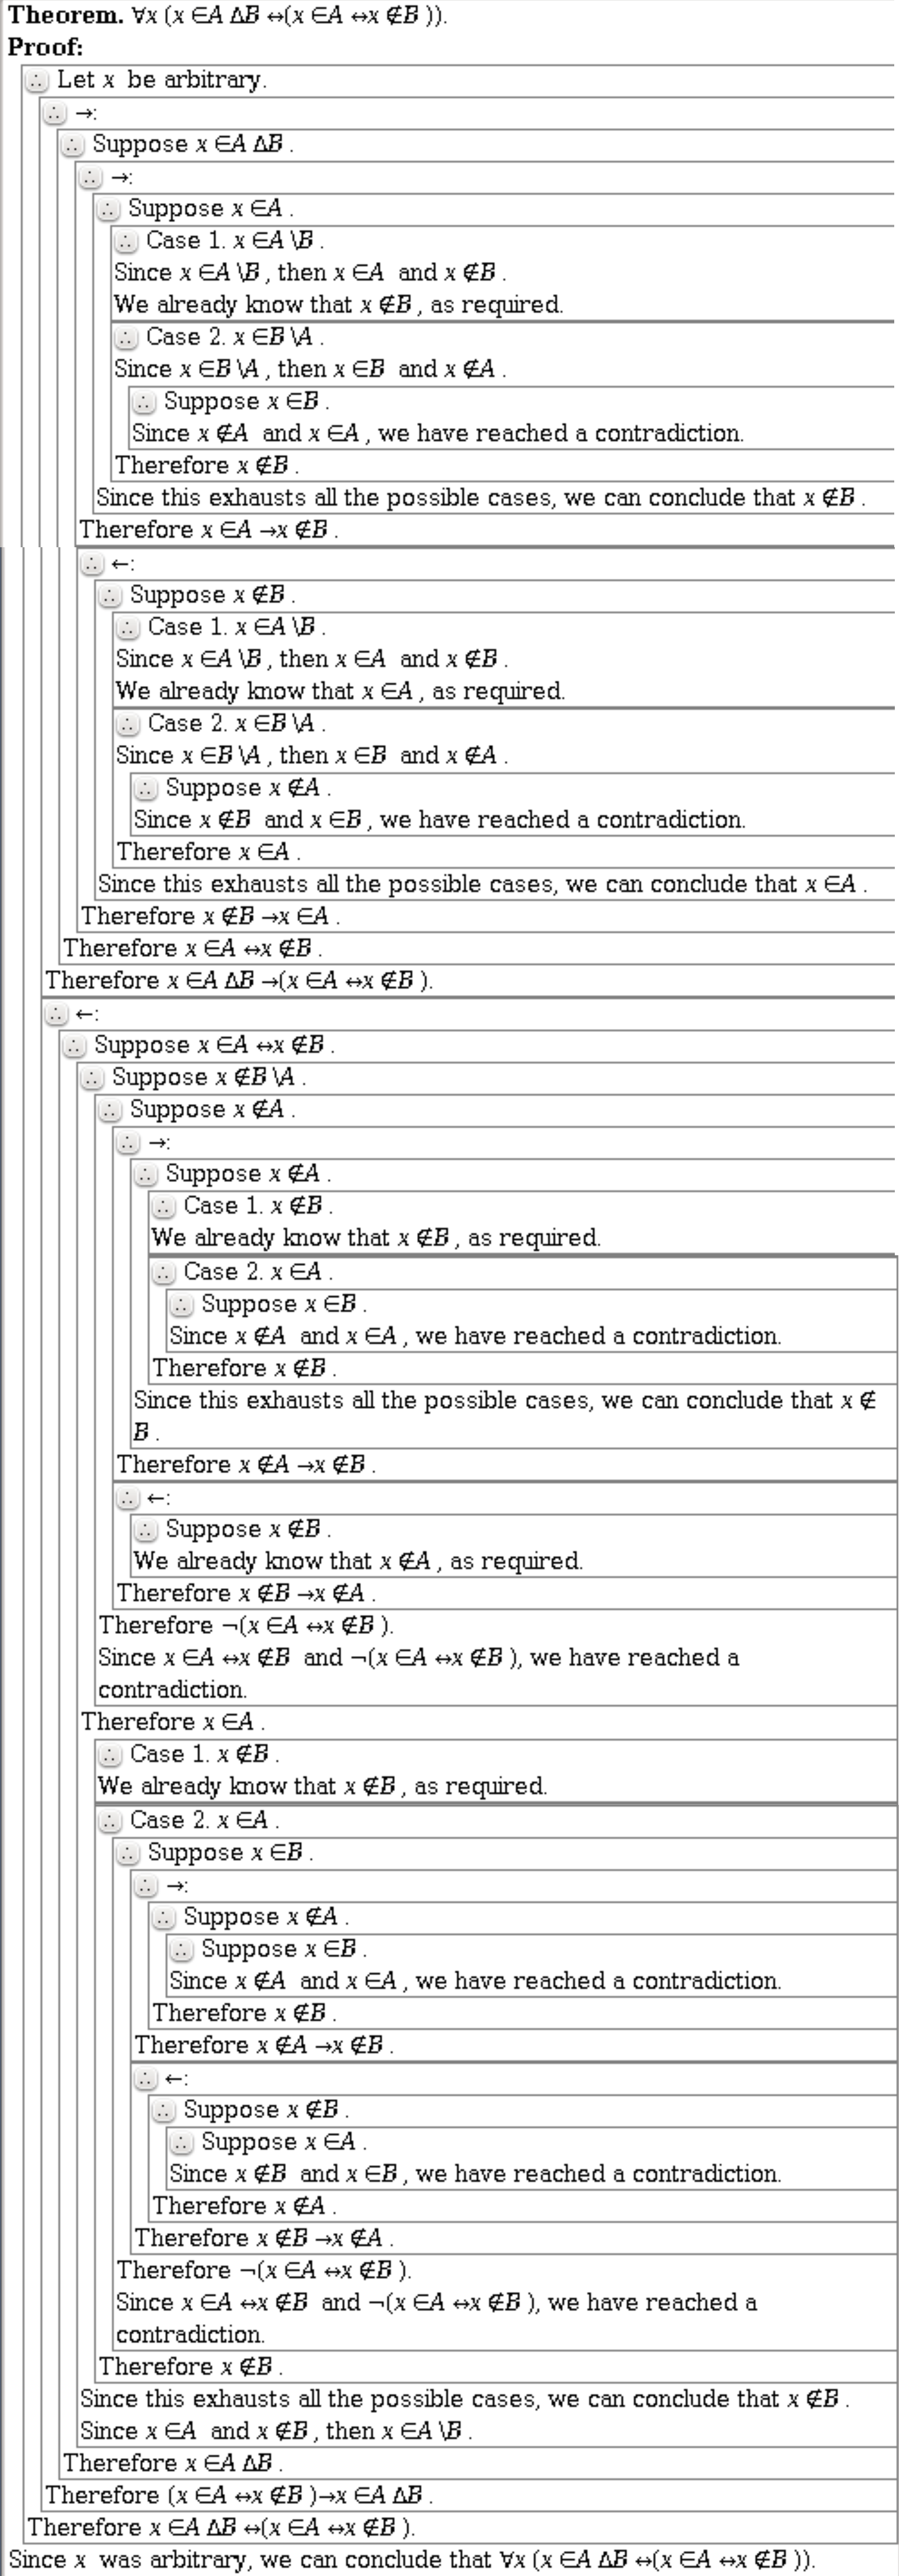
\includegraphics[scale=0.12]{3_5_18}

\vspace{30pt}

$^{\textit{P}}_{\, \textit{D}}$ *19. Suppose A, B, and C are sets. Prove that $A \Delta B$ and C are disjoint iff
$A \cap C = B \cap C$.

\vspace{30pt}

\textbf{3.5.19.pd}
\vspace{10pt}

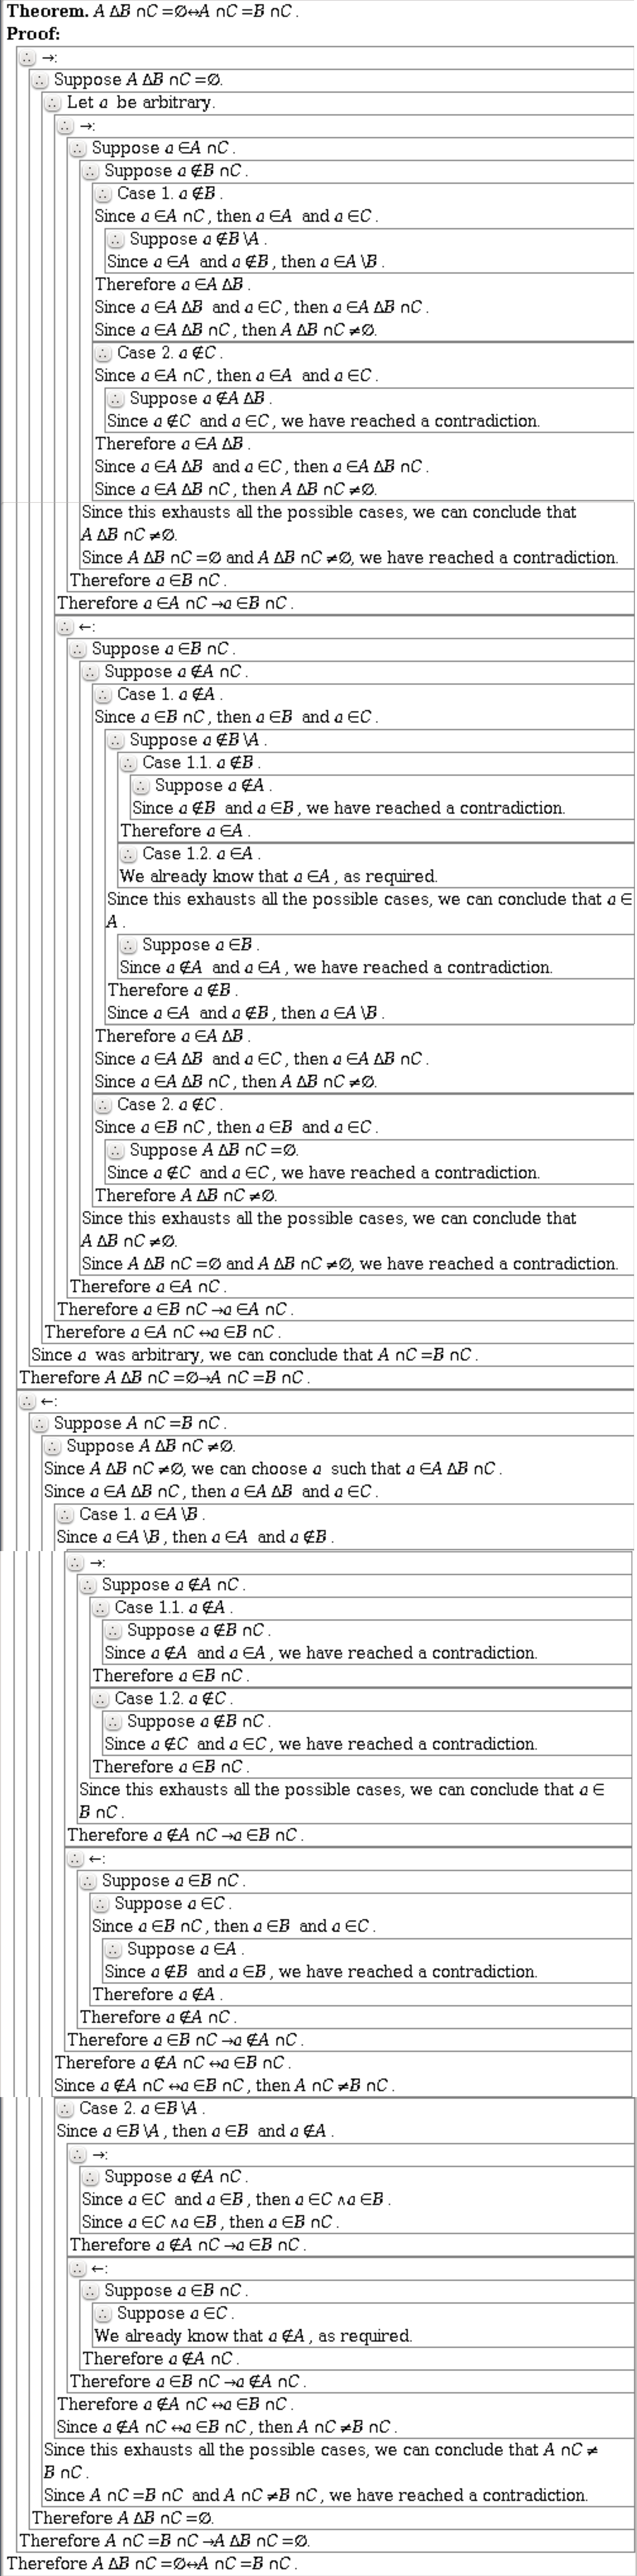
\includegraphics[scale=0.09]{3_5_19}

\vspace{30pt}

$^{\textit{P}}_{\, \textit{D}}$ 20. Suppose A, B, and C are sets. Prove that $A \Delta B \subseteq C$ iff $A \cup C = B \cup C$.

\vspace{30pt}

\textbf{3.5.20.pd}
\vspace{10pt}

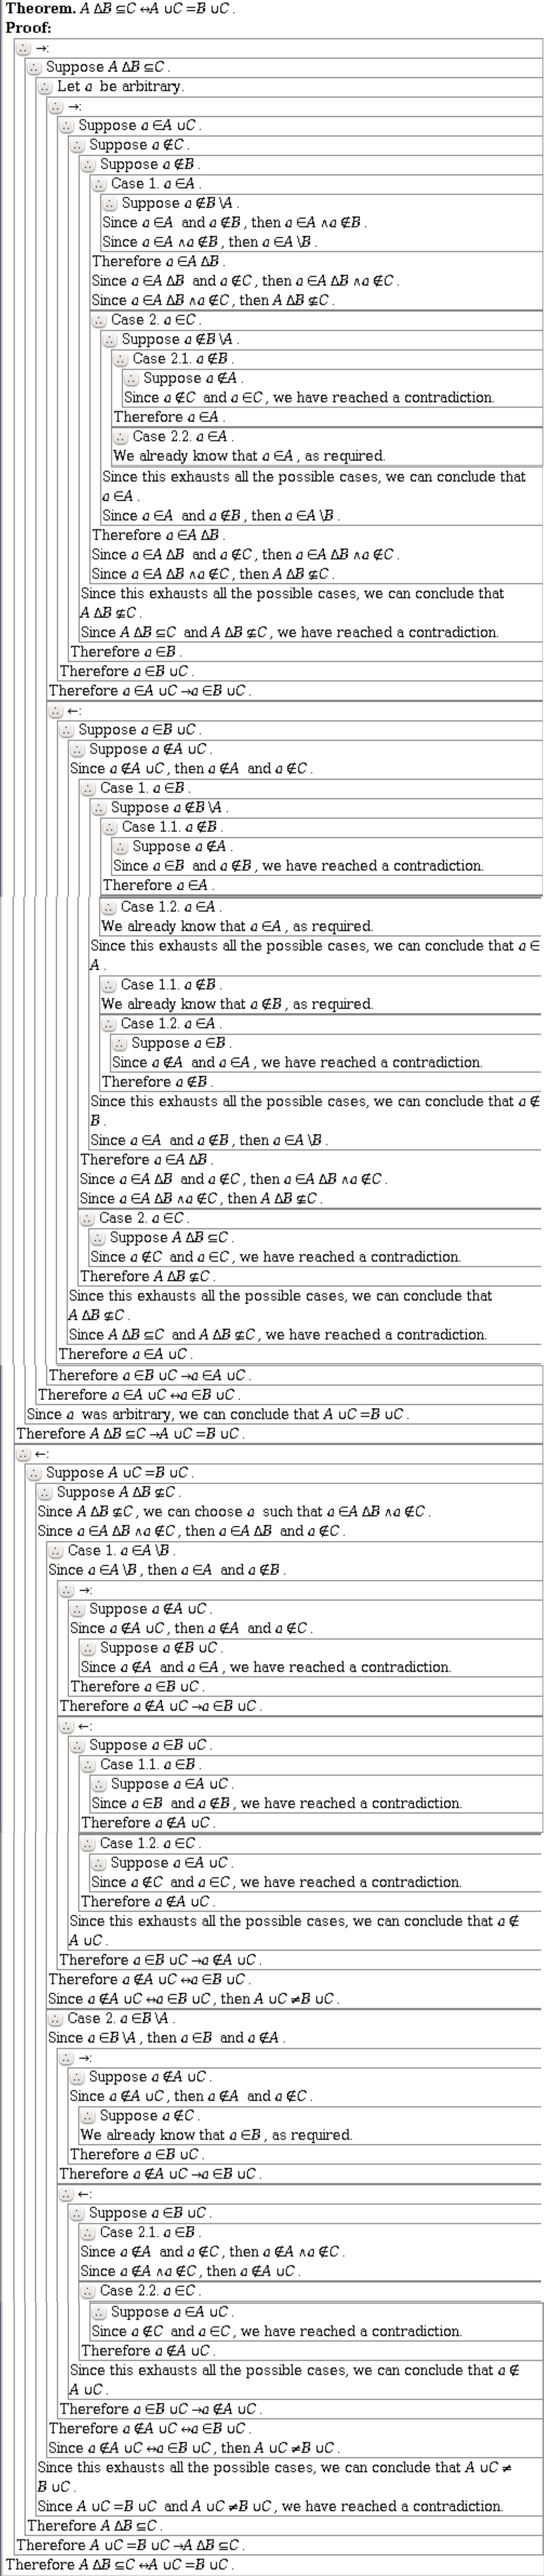
\includegraphics[scale=0.08]{3_5_20}

\vspace{30pt}

$^{\textit{P}}_{\, \textit{D}}$ 21. Suppose A, B, and C are sets. Prove that $C \subseteq A \Delta B$ iff $C \subseteq A \cup B$ and $A \cap B \cap C = \varnothing$.

\vspace{30pt}

\textbf{3.5.21.pd}
\vspace{10pt}

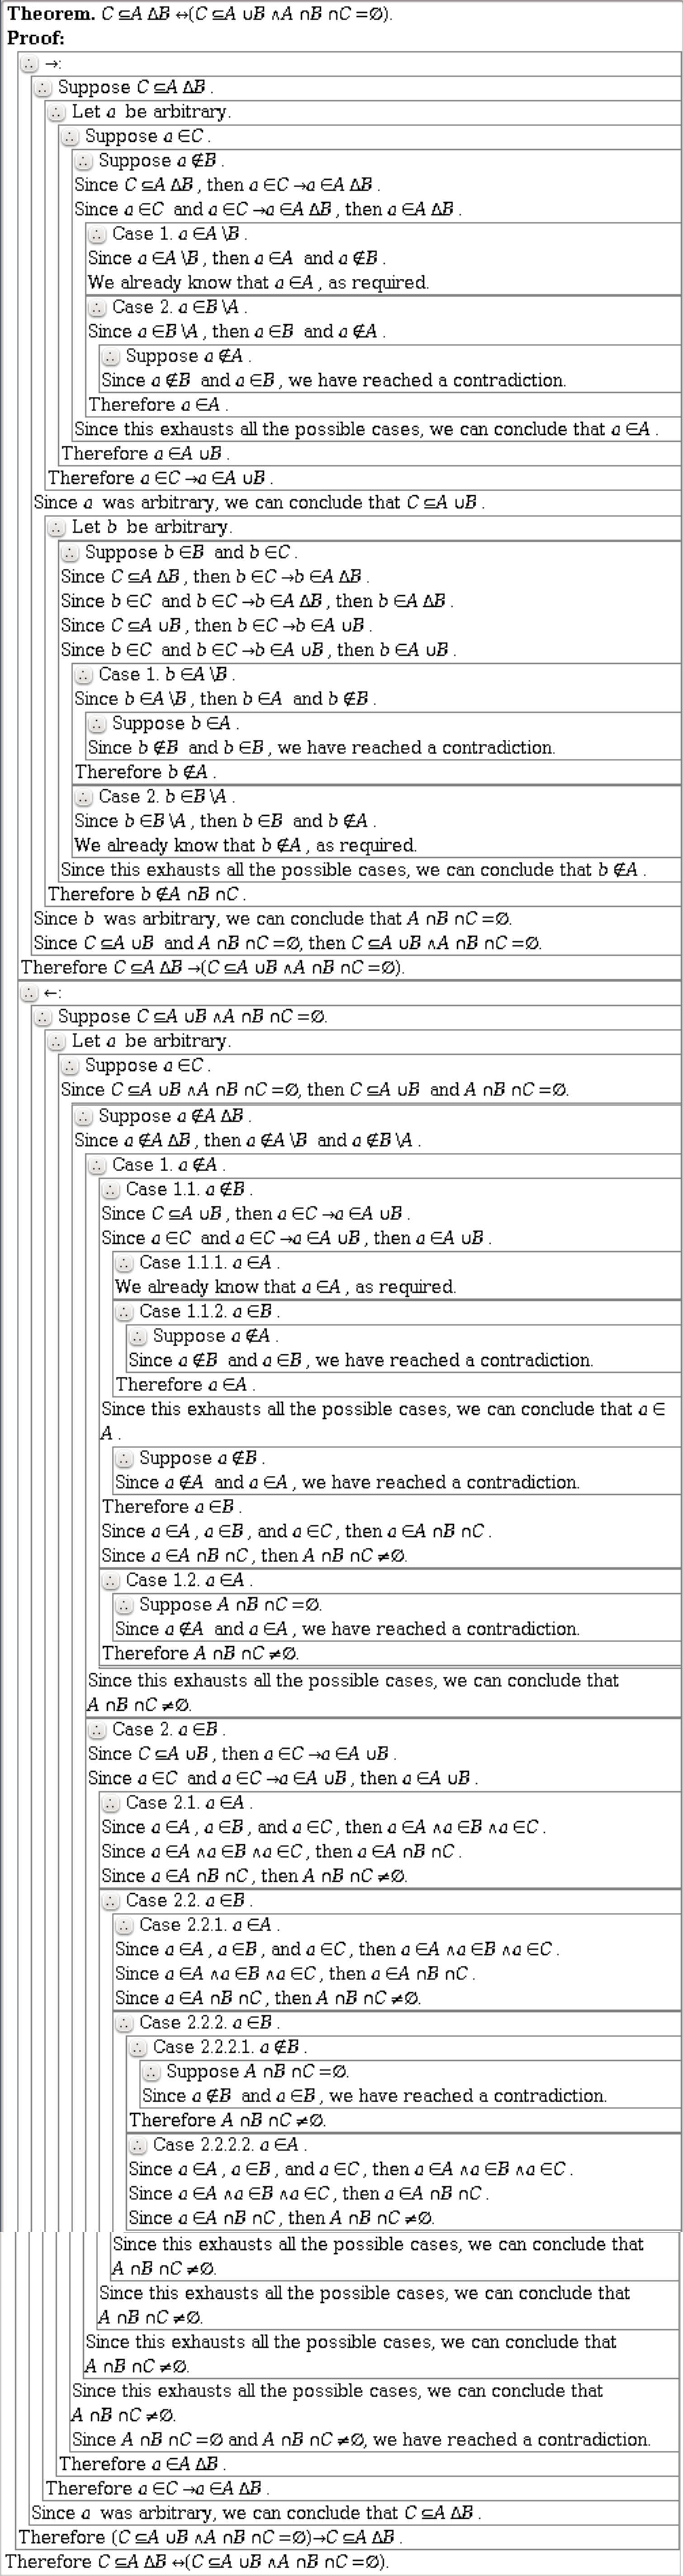
\includegraphics[scale=0.08]{3_5_21}

\vspace{30pt}

$^{\textit{P}}_{\, \textit{D}}$ *22. Suppose A, B, and C are sets.

\hspace{12pt}(a) Prove that $A \setminus C \subseteq (A \setminus B) \cup (B \setminus C)$.

\hspace{12pt}(b) Prove that $A \Delta C \subseteq (A \Delta B) \cup (B \Delta C)$.

\vspace{30pt}

(a)


\textbf{3.5.22.1.pd}
\vspace{10pt}

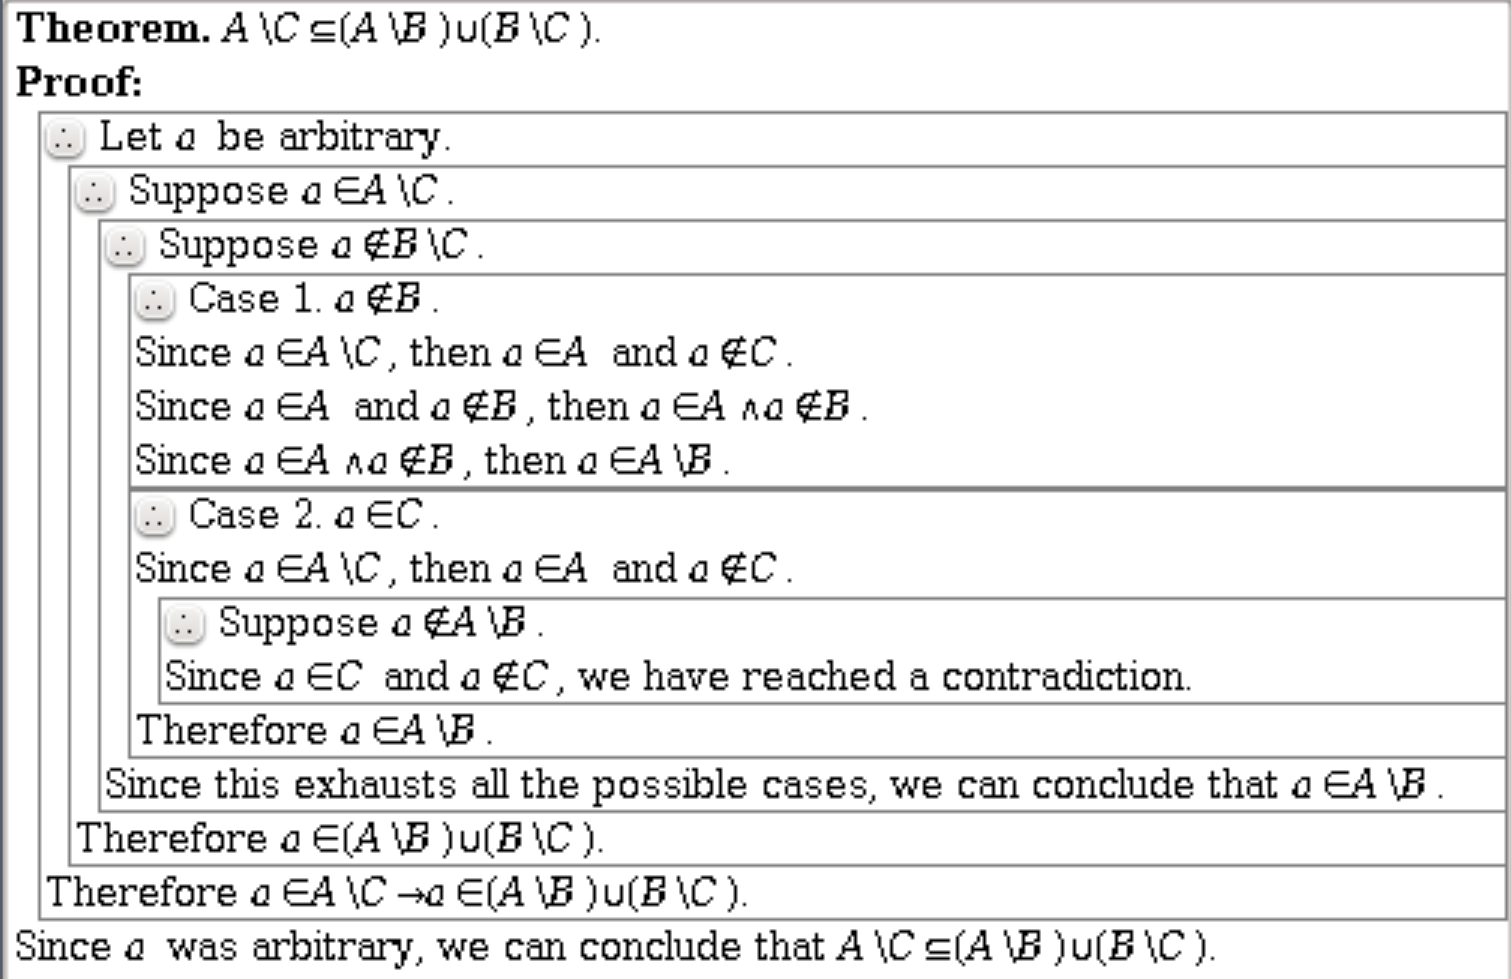
\includegraphics[width=\textwidth]{3_5_22_1}

\vspace{30pt}

(b)

\textbf{3.5.22.2.pd}
\vspace{10pt}

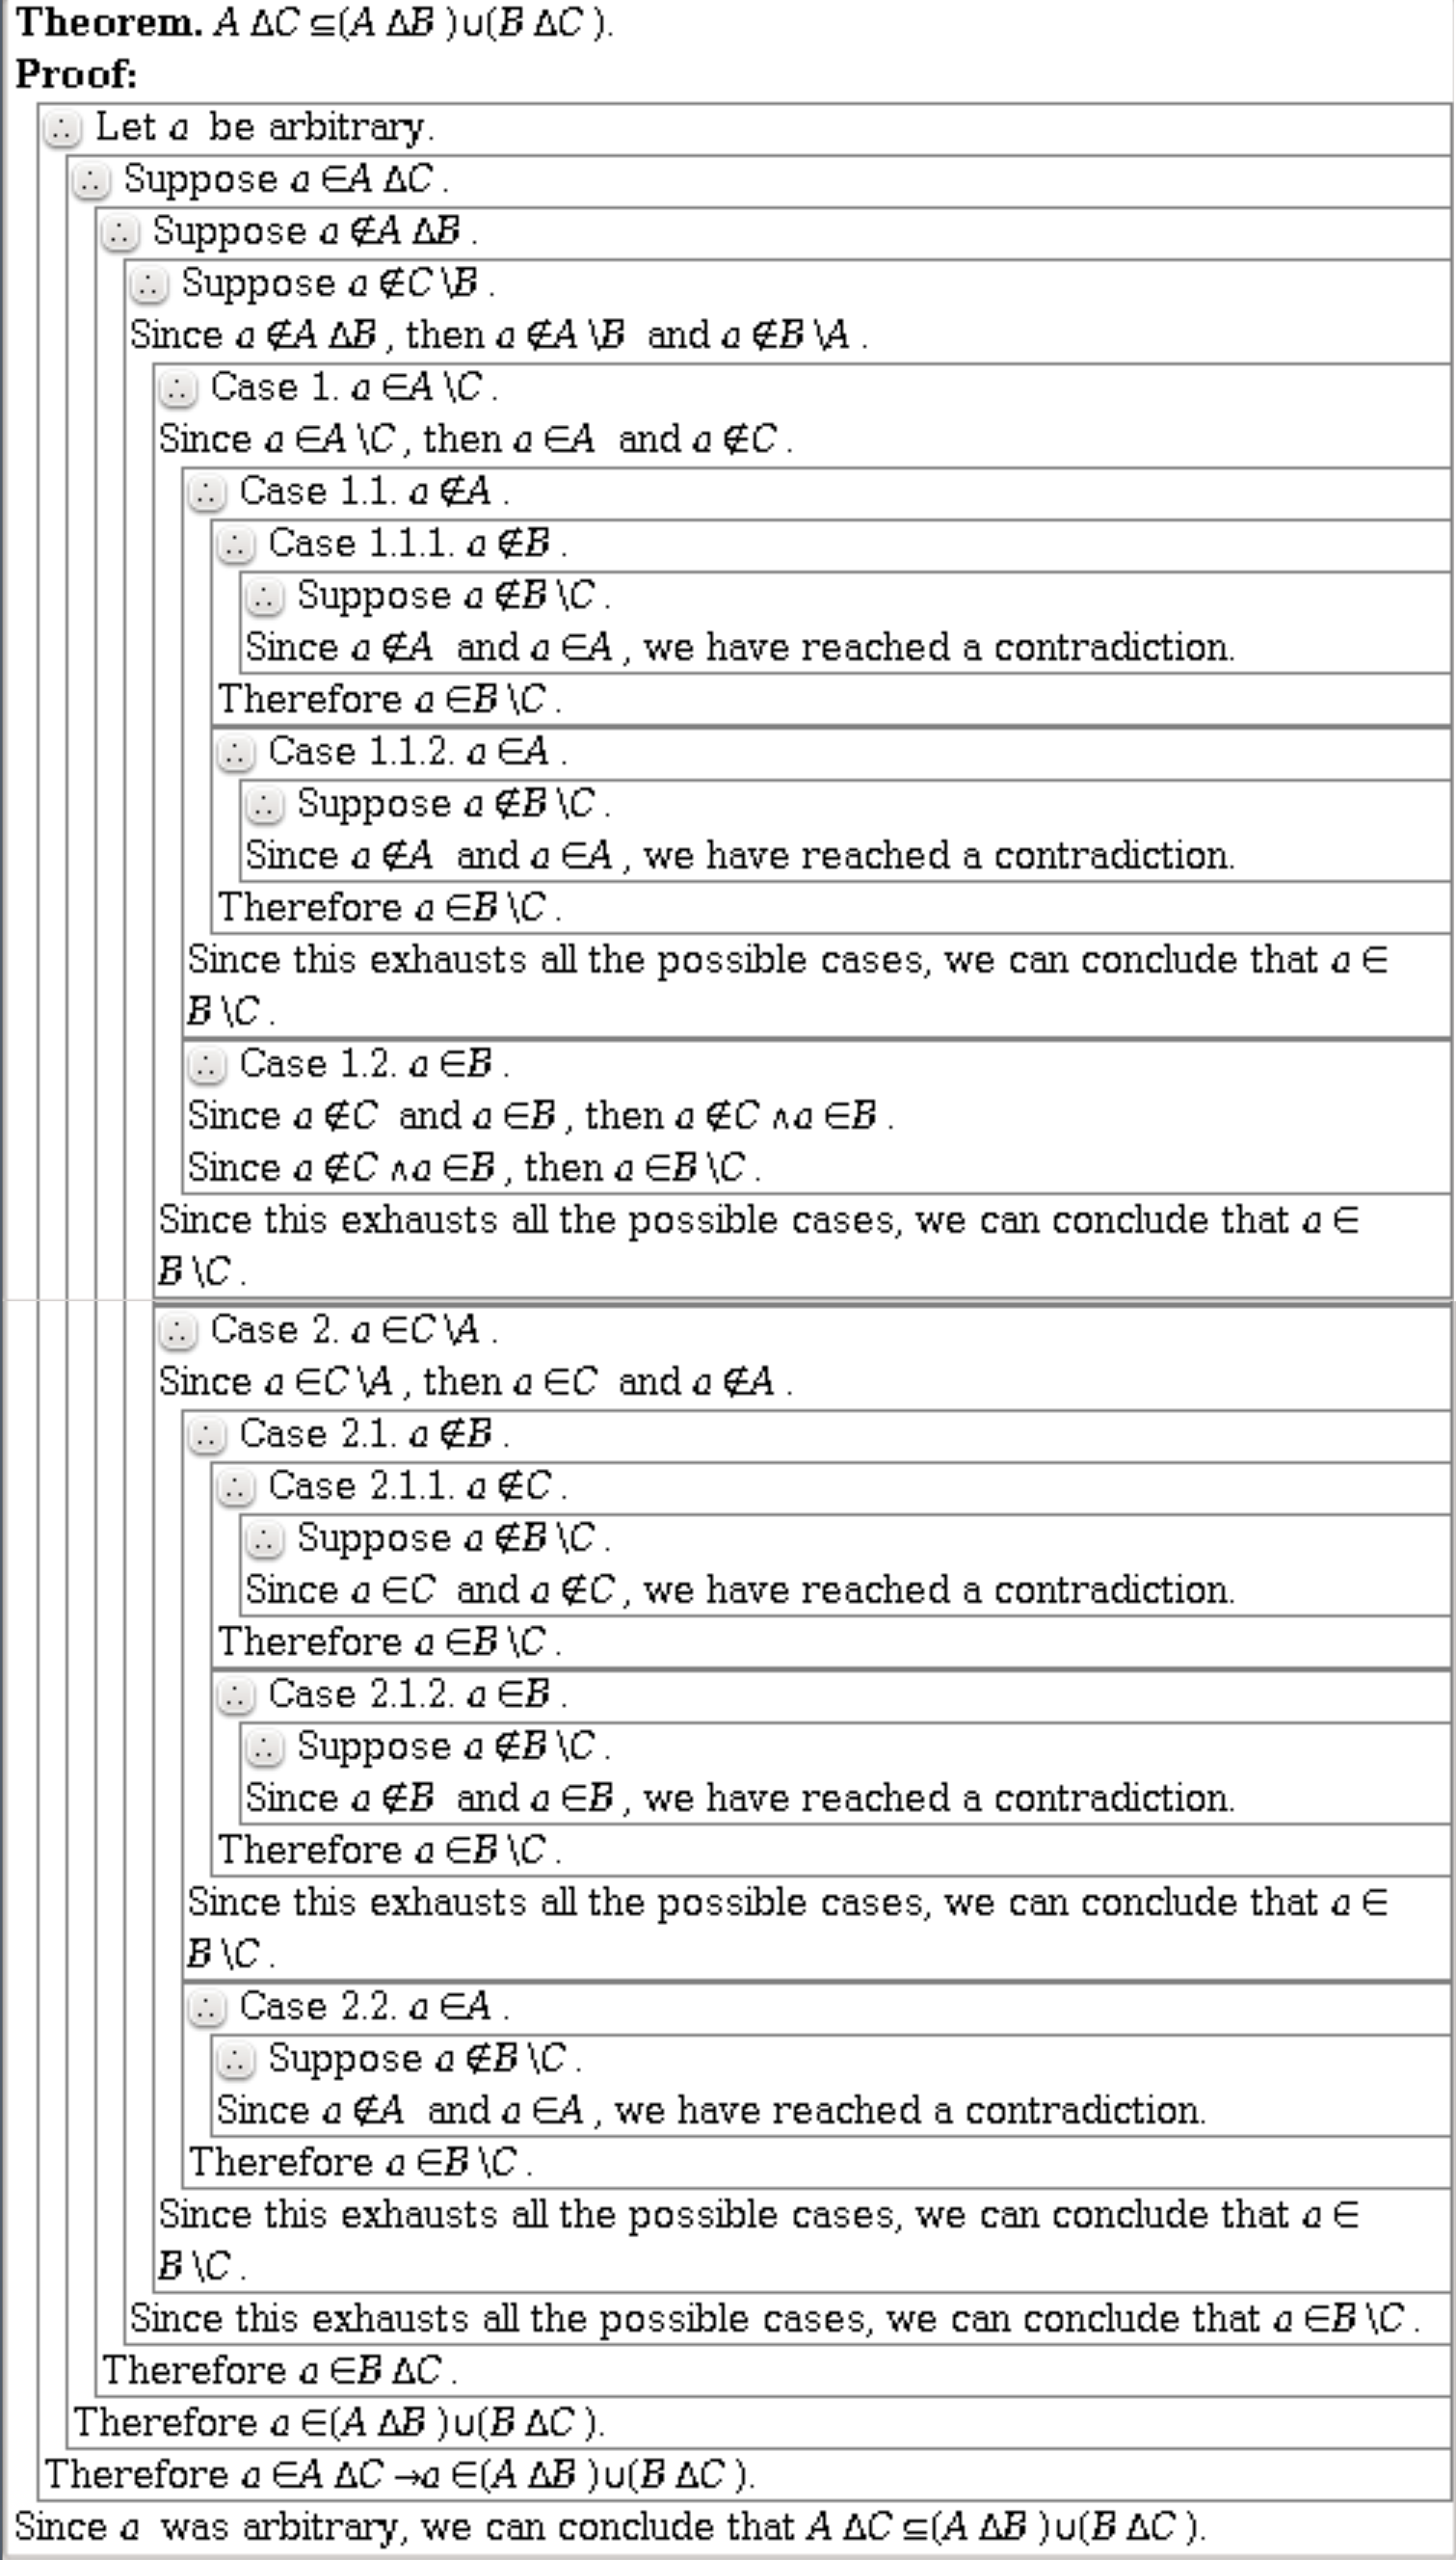
\includegraphics[width=\textwidth]{3_5_22_2}

\vspace{30pt}

$^{\textit{P}}_{\, \textit{D}}$ *23. Suppose A, B, and C are sets.

\hspace{12pt}(a) Prove that $(A \cup B) \Delta C \subseteq (A \Delta C) \cup (B \Delta C)$.

\hspace{12pt}(b) Find an example of sets A, B, and C such that $(A \cup B) \Delta C \neq
(A \Delta C) \cup (B \Delta C)$

\vspace{30pt}

(a)

\textbf{3.5.23.1.pd}
\vspace{10pt}

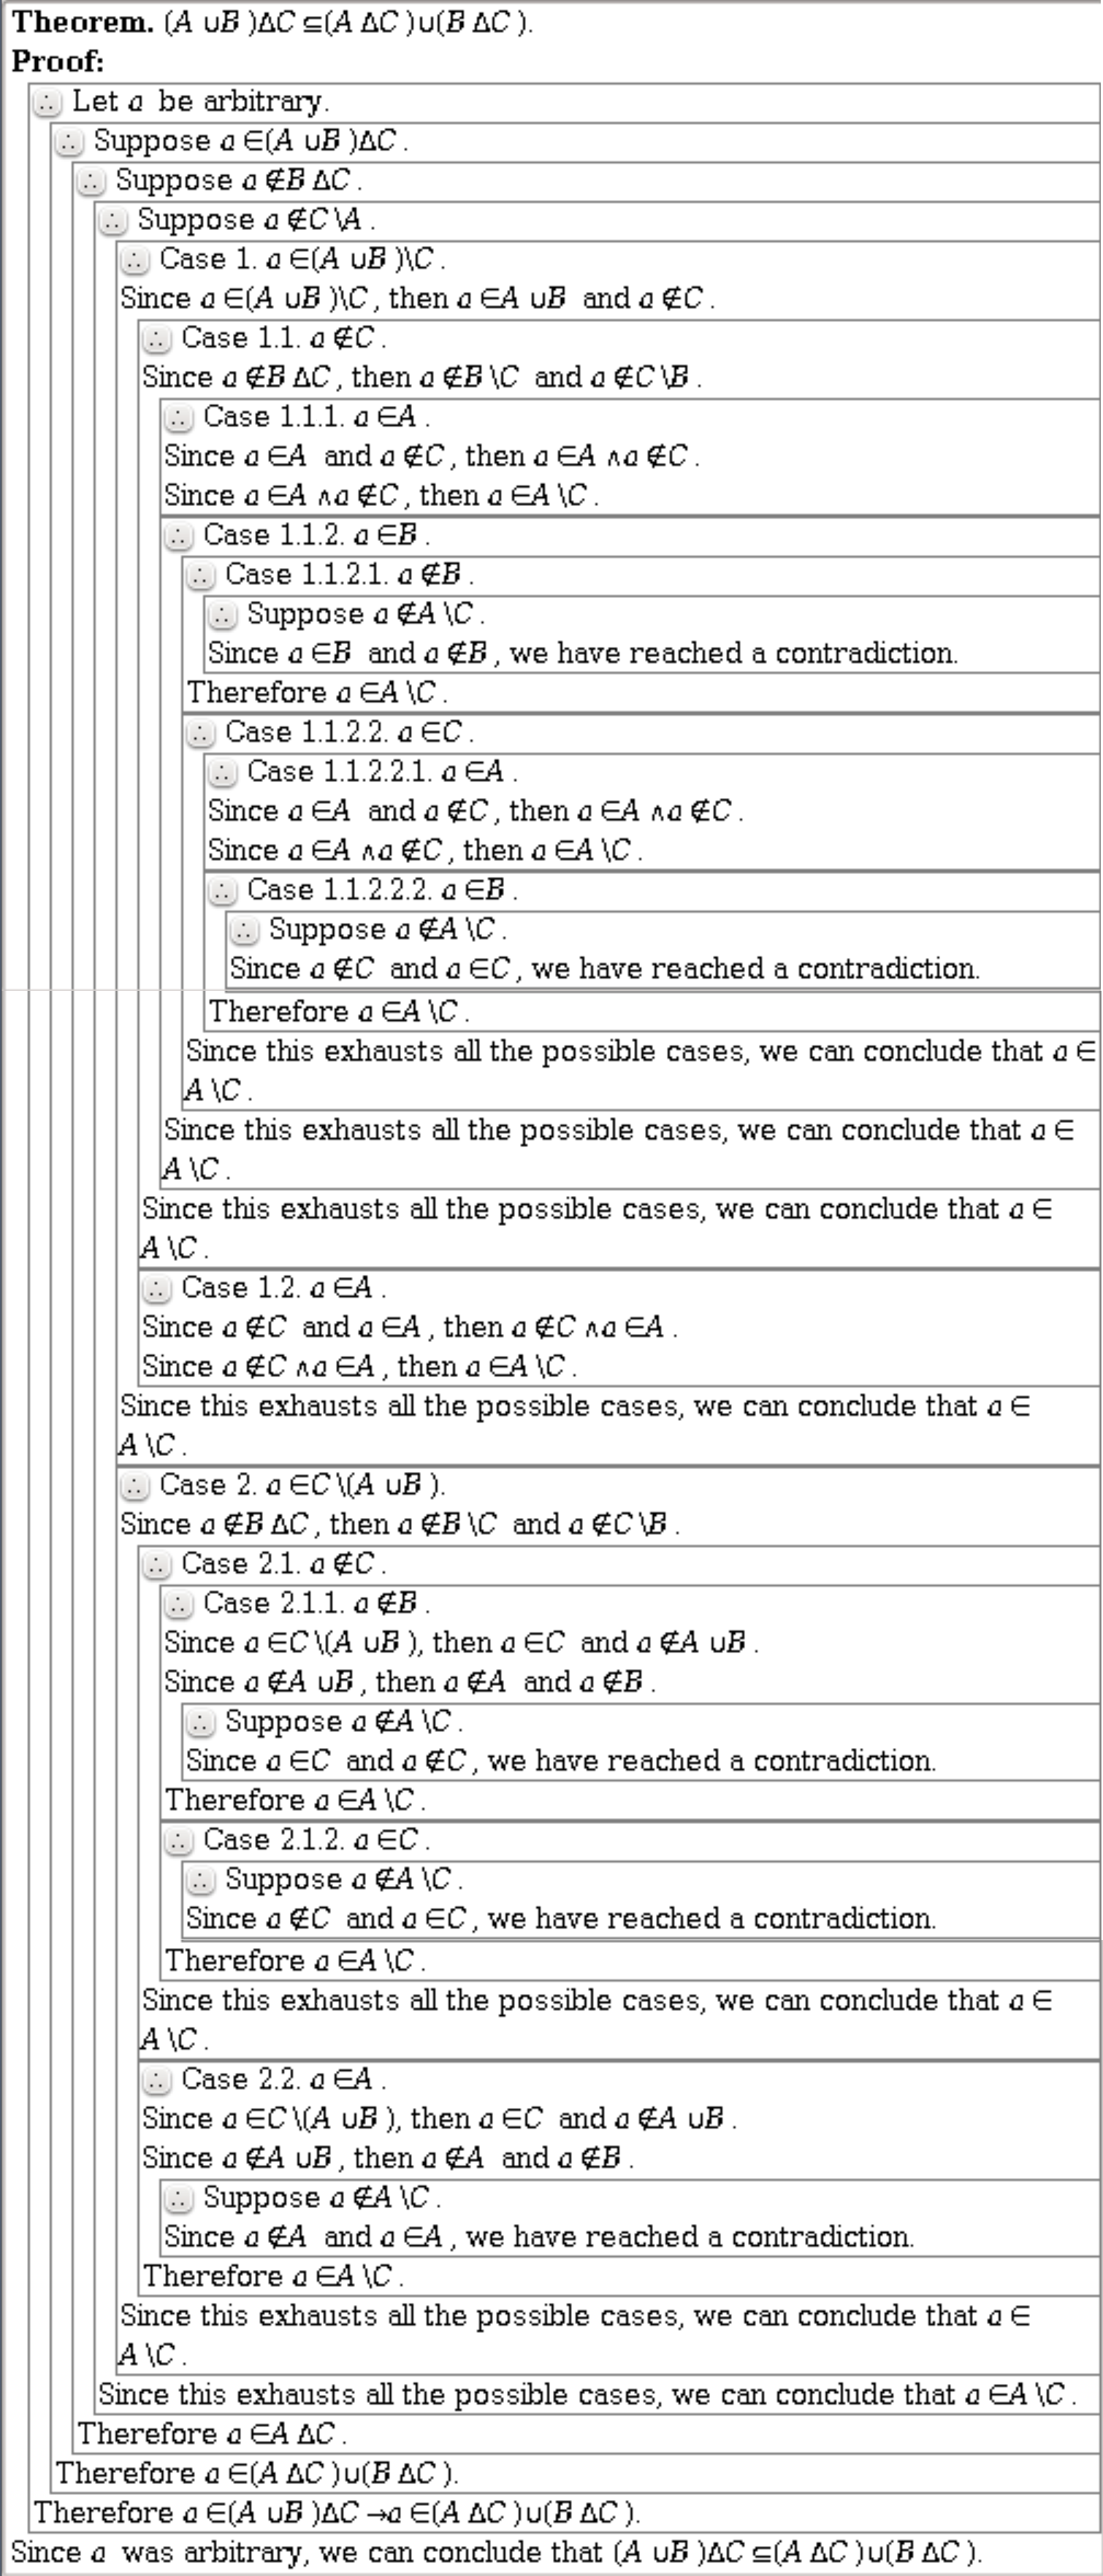
\includegraphics[scale=0.15]{3_5_23_1}

\vspace{30pt}

(b)

$A = \{1,2\}$

$B = \{1\}$

$C = \{2\}$

$A \cup B = \{1, 2\}$

$\{1,2\} \Delta \{2\} = (\{1,2\} \cup \{2\}) \setminus (\{1,2\} \cap \{2\}) = \{1,2\} \setminus \{2\} = \{1\}$

$A \Delta C = (\{1,2\} \cup \{2\}) \setminus (\{1,2\} \cap \{2\}) = \{1,2\} \setminus \{2\} = \{1\}$

$B \Delta C = \{1,2\} \setminus \{\varnothing\} = \{1,2\}$

$\{1\} \cup \{1,2\} = \{1,2\}$

$(A \cup B) \Delta C \neq (A \Delta C) \cup (B \Delta C)$

$\{1\} \neq \{1,2\}$


\vspace{30pt}

$^{\textit{P}}_{\, \textit{D}}$ 24. Suppose A, B, and C are sets.

\hspace{12pt}(a) Prove that $(A \Delta C) \cap (B \Delta C) \subseteq (A \cap B) \Delta C$.

\hspace{12pt}(b) Is it always true that $(A \cap B) \Delta C \subseteq (A \Delta C) \cap (B \Delta C)$? Give
either a proof or a counterexample.

\vspace{30pt}

(a)

\textbf{3.5.24.1.pd}
\vspace{10pt}

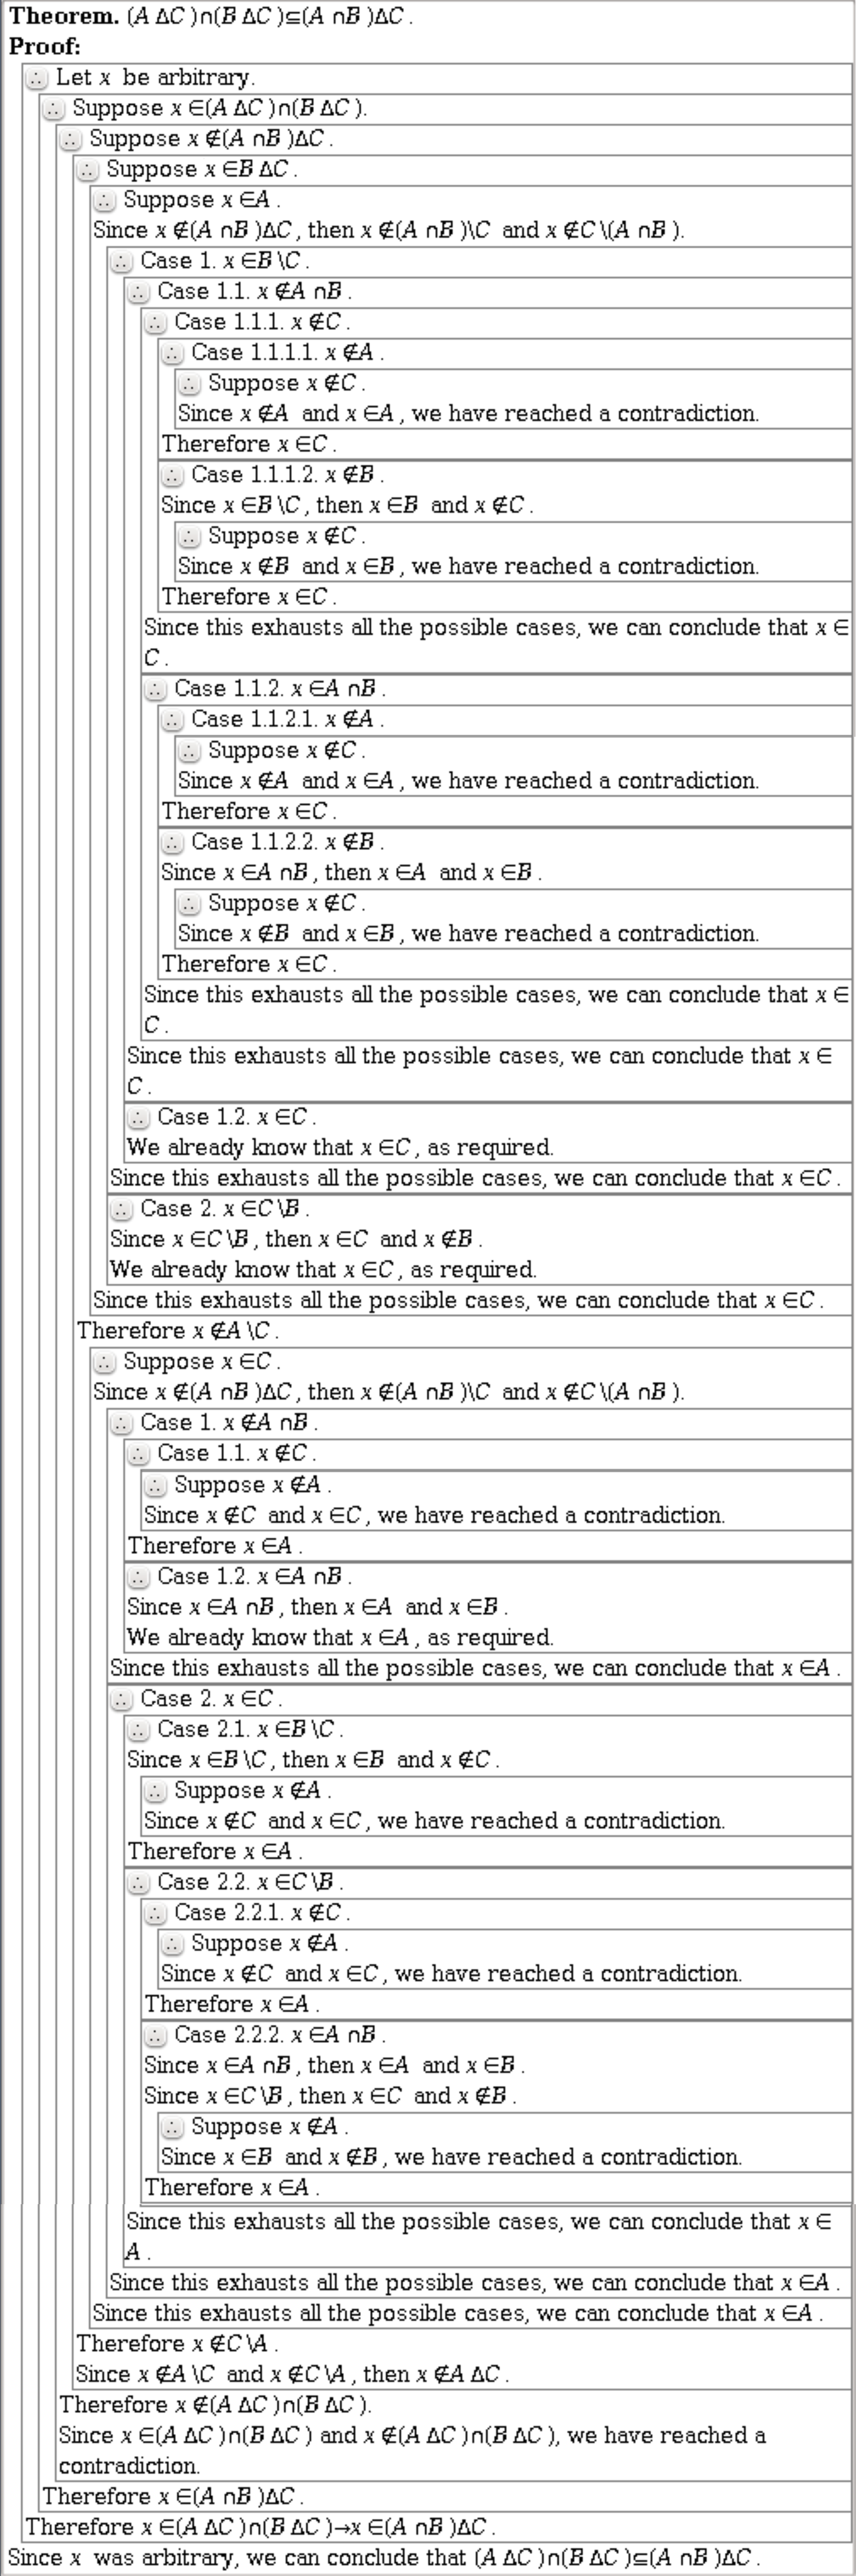
\includegraphics[scale=0.10]{3_5_24_1}

\vspace{30pt}

(b)

$A = \{1,2\}$

$B = \{1\}$

$C = \{2\}$

$A \cap B = \{1\}$

$\{1\} \Delta \{2\} = \{1,2\} \setminus \{\varnothing\} = \{1,2\}$

$A \Delta C = (\{1,2\} \cup \{2\}) \setminus (\{1,2\} \cap \{2\}) = \{1,2\} \setminus \{2\} = \{1\}$

$B \Delta C = \{1,2\} \setminus \{\varnothing\} = \{1,2\}$

$\{1\} \cap \{1,2\} = \{1\}$

$(A \cap B) \Delta C \nsubseteq (A \Delta C) \cap (B \Delta C)$

$\{1,2\} \nsubseteq \{1\}$


\vspace{30pt}

$^{\textit{P}}_{\, \textit{D}}$ 25. Suppose A, B, and C are sets. Consider the sets $(A \setminus B) \Delta C$ and
$(A \Delta C) \setminus (B \Delta C)$. Can you prove that either is a subset of the other?
Justify your conclusions with either proofs or counterexamples.

\vspace{30pt}

\textbf{3.5.25.pd}
\vspace{10pt}

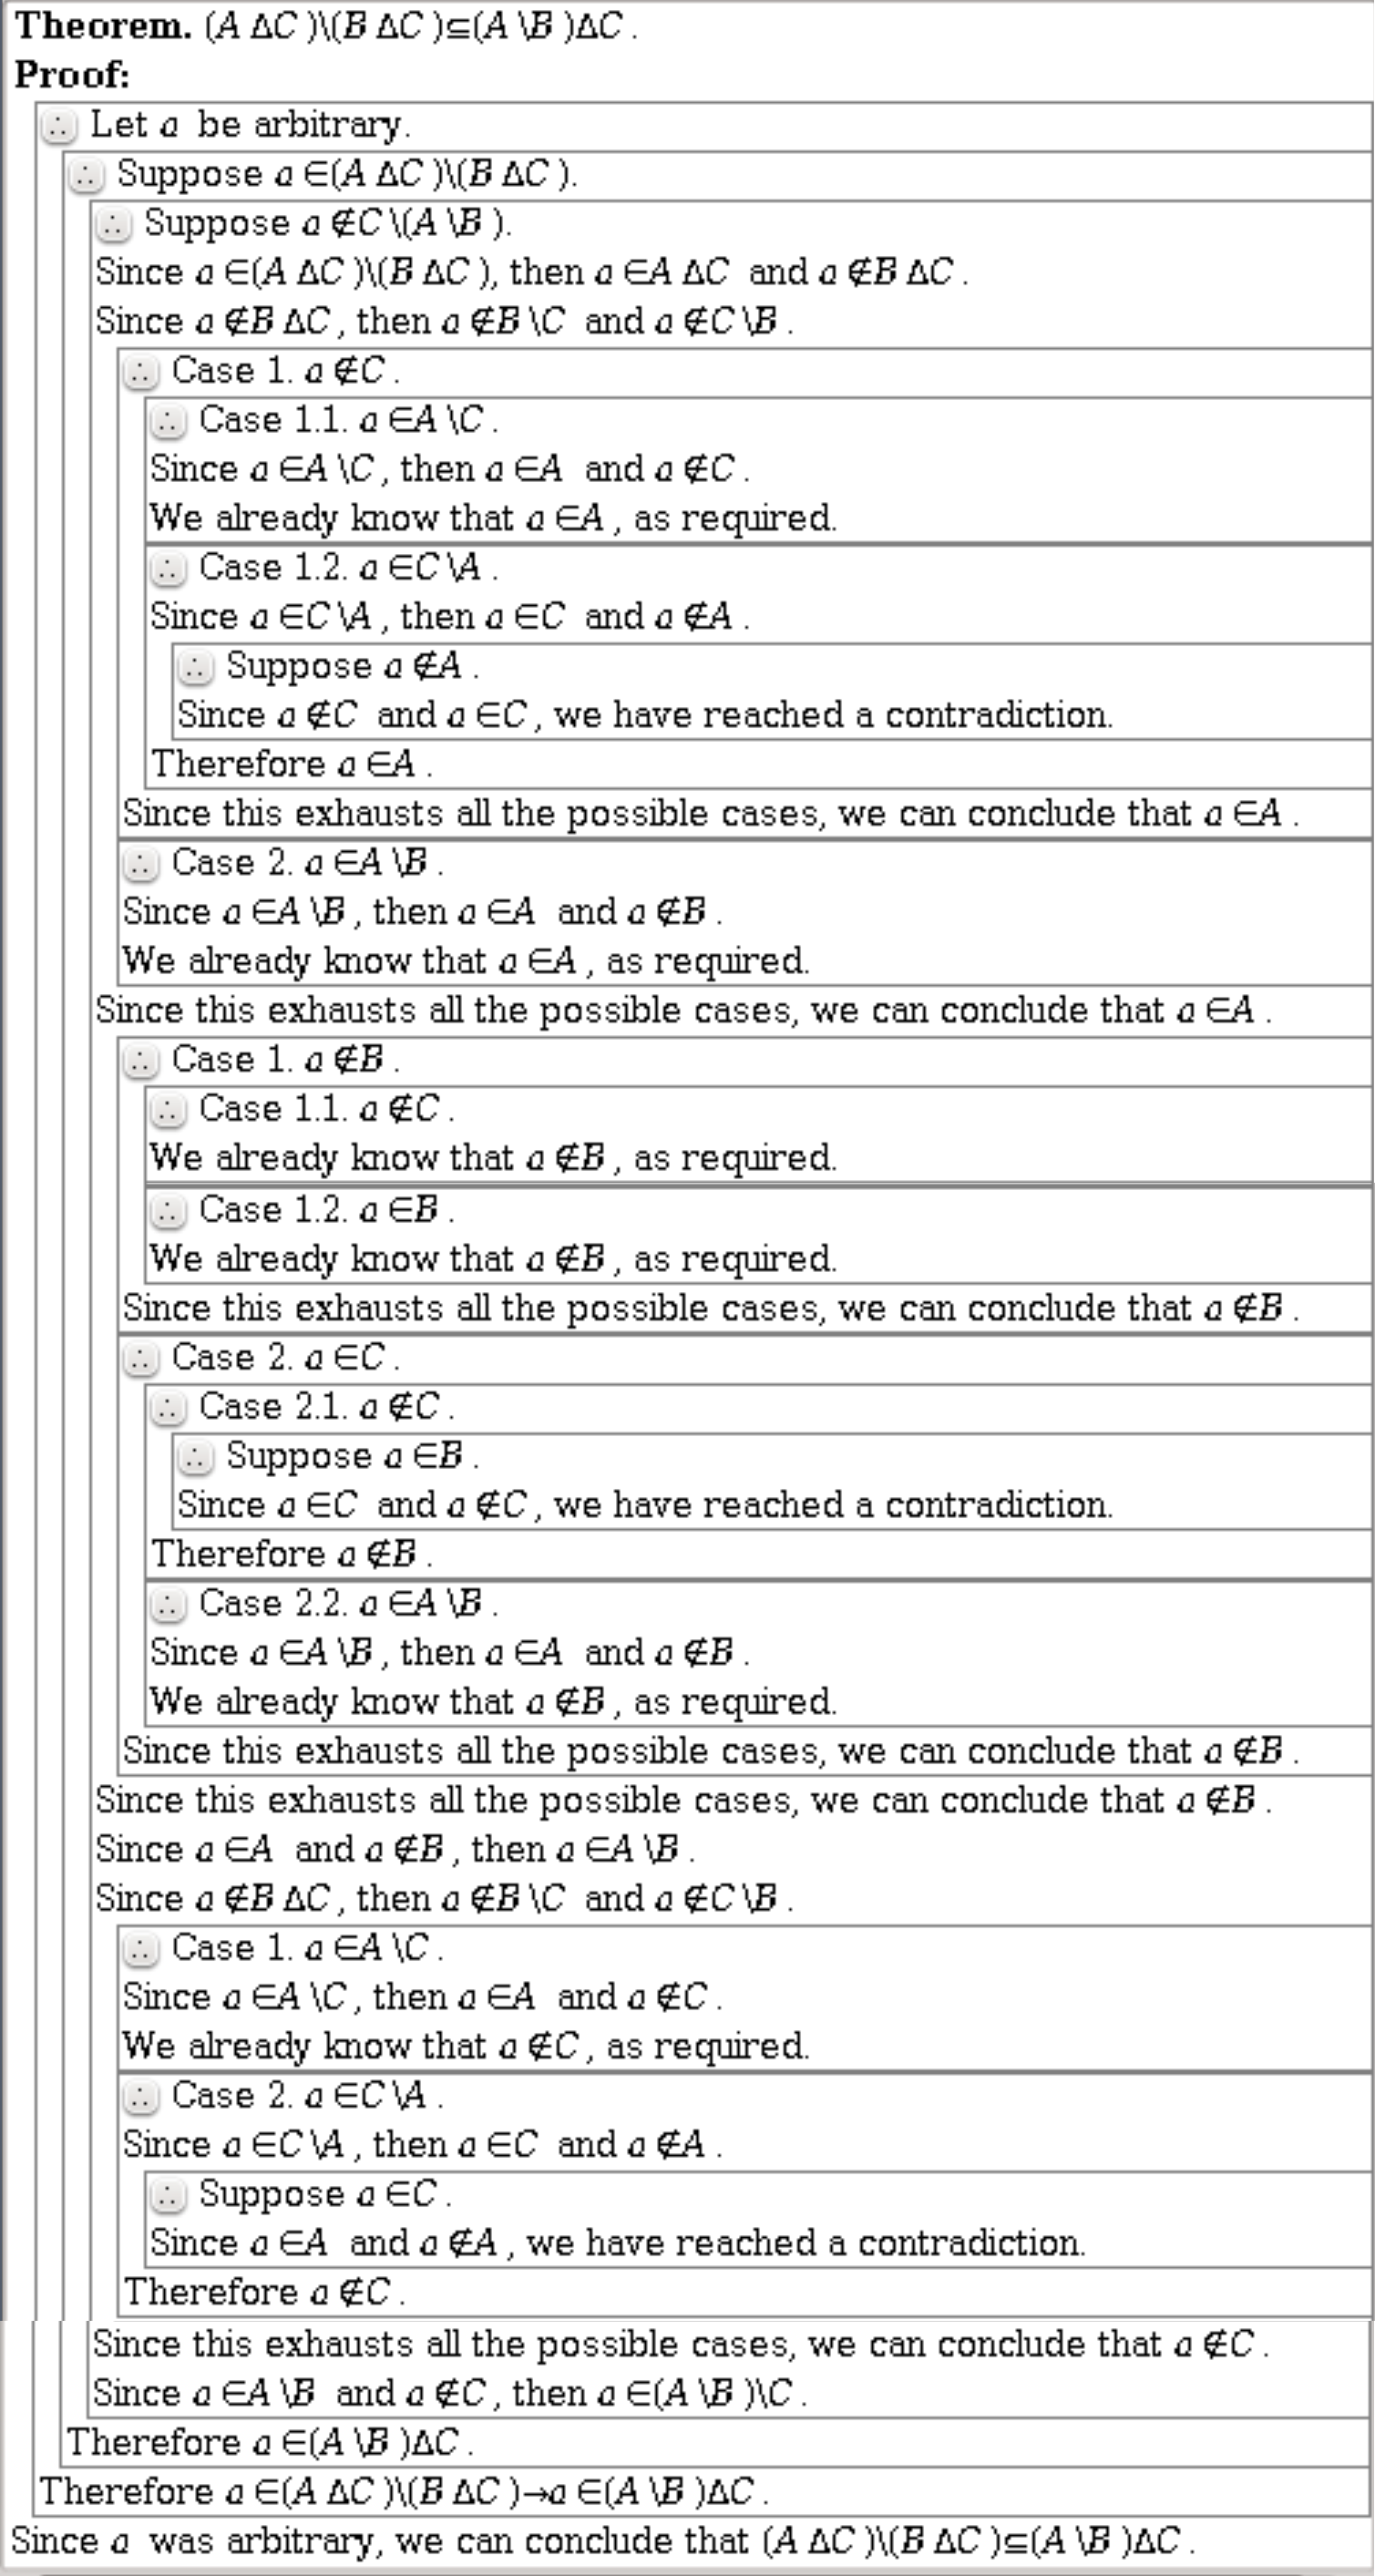
\includegraphics[scale=0.15]{3_5_25}

$(A \setminus B) \Delta C \nsubseteq (A \Delta C) \setminus (B \Delta C)$

$A = \{1,2\}$

$B = \{1\}$

$C = \{1,2\}$

$A \setminus B = \{2\}$

$\{2\} \Delta \{1,2\} = \{1,2\} \setminus \{2\} = \{1\}$

$A \Delta C = \{1,2\} \setminus \{1,2\} = \{\varnothing\}$

$B \Delta C = \{1,2\} \setminus \{1\} = \{2\}$

$\{\varnothing\} \setminus \{2\} = \{\varnothing\}$

$(A \cap B) \Delta C \nsubseteq (A \Delta C) \cap (B \Delta C)$

$\{1\} \nsubseteq \{\varnothing\}$

\vspace{30pt}

*26. Consider the following putative theorem.

\textbf{Theorem?} For every real number x, if $|x - 3| < 3$ then $0 < x < 6$.

Is the following proof correct? If so, what proof strategies does it use?
If not, can it be fixed? Is then theorem correct?

\textit{Proof.} Let x be an arbitrary real number, and suppose $|x - 3| < 3$. We
consider two cases:

\textit{Case} 1. $x - 3 \geq 0$. Then $|x - 3| = x - 3$. Plugging this into the assumption
that $|x - 3| < 3$, we get $x - 3 < 3$, so clearly $x < 6$.

\textit{Case} 2. $x - 3 < 0$. Then $|x - 3| = 3 - x$, so the assumption $|x - 3| < 3$ means that $3 - x < 3$. Therefore $3 < 3 + x$, so $0 < x$.

Since we have proven both $0 < x$ and $x < 6$, we can conclude that $0 < x < 6$.

\vspace{30pt}

\centerline{
  \begin{tabular}{l l}
  \textit{Givens} & \textit{Goal} \\
    $$ & $\forall x (|x - 3| < 3 \to 0 < x < 6)$ \\
 \end{tabular}}
\vspace{10pt}

\centerline{
  \begin{tabular}{l l}
  \textit{Givens} & \textit{Goal} \\
    $$ & $|x - 3| < 3 \to 0 < x < 6$ \\
 \end{tabular}}
\vspace{10pt}

\centerline{
  \begin{tabular}{l l}
  \textit{Givens} & \textit{Goal} \\
    $|x - 3| < 3$ & $0 < x < 6$ \\
 \end{tabular}}
\vspace{10pt}

$|x - 3| < 3$ 

Case 1.

$x - 3 \geq 0$

$x - 3 < 3$

$x < 6$

Case 2.

$x - 3 < 0$

$x < 3$

$3 - x < 3$

$x > 0$

Proof is wrong, since it proved only that $x < 6$ or $x > 0$, but not $x < 6$ and $x > 0$.

Fixed flow.

\centerline{
  \begin{tabular}{l l}
  \textit{Givens} & \textit{Goal} \\
    $|x - 3| < 3$ & $0 < x < 6$ \\
 \end{tabular}}
\vspace{10pt}

Case 1. $x - 3 > 0$

$x - 3 < 3$

$x < 6$

$x < 6$ and $x > 3$

$3 < x < 6$ 

Case 2

$x - 3 < 0$

$x < 3$

$x > 0$ and $x < 3$

$0 < x < 3$

Since $3 < x < 6$ or $0 < x < 3$, it follows that $0 < x < 6$.

\vspace{30pt}

27. Consider the following putative theorem.

\textbf{Theorem?} For any sets A, B, and C, if $A \setminus B \subseteq C$ and $A \nsubseteq C$ then
$A \cap B \neq \varnothing$.

Is the following proof correct? If so, what proof strategies does it use?
If not, can it be fixed? Is the theorem correct?

\textit{Proof.} Since $A \nsubseteq C$, we can choose some x such that $x \in A$ and $x \notin C$.
Since $x \notin C$ and $A \setminus B \subseteq C$, $x \notin A \setminus B$. Therefore either $x \notin A$ or
$x \in B$. But we already know that $x \in A$, so it follows that $x \in B$. Since
$x \in A$ and $x \in B$, $x \in A \cap B$. Therefore $A \cap B \neq \varnothing$.

\vspace{30pt}

\centerline{
  \begin{tabular}{l l}
  \textit{Givens} & \textit{Goal} \\
    $$ & $(A \setminus B \subseteq C) \text{ and } (A \nsubseteq C) \to A \cap B \neq \varnothing$ \\
 \end{tabular}}
\vspace{10pt}

\centerline{
  \begin{tabular}{l l}
  \textit{Givens} & \textit{Goal} \\
    $A \setminus B \subseteq C$ & $A \cap B \neq \varnothing$ \\
    $A \nsubseteq C$ & \\
 \end{tabular}}
\vspace{10pt}

$A \nsubseteq C$

$\neg \forall x (x \in A \to x \in C)$

$\exists x (x \in A \land x \notin C)$

\centerline{
  \begin{tabular}{l l}
  \textit{Givens} & \textit{Goal} \\
    $A \setminus B \subseteq C$ & $A \cap B \neq \varnothing$ \\
    $x \in A$ & \\
    $x \notin C$ & \\
 \end{tabular}}
\vspace{10pt}

$A \setminus B \subseteq C$

$\forall x (x \in A \setminus B \to x \in C)$

\centerline{
  \begin{tabular}{l l}
  \textit{Givens} & \textit{Goal} \\
    $x \notin A \setminus B$ & $A \cap B \neq \varnothing$ \\
    $x \in A$ & \\
    $x \notin C$ & \\
 \end{tabular}}
\vspace{10pt}

$\neg (x \in A \land x \notin B)$
$x \notin A \lor x \in B$

\centerline{
  \begin{tabular}{l l}
  \textit{Givens} & \textit{Goal} \\
    $x \notin A \lor x \in B$ & $A \cap B \neq \varnothing$ \\
    $x \in A$ & \\
    $x \notin C$ & \\
 \end{tabular}}
\vspace{10pt}

Since $x \notin A \lor x \in B$ and $x \in A$, $x \in B$ (Disjunctive Syllogism).

\centerline{
  \begin{tabular}{l l}
  \textit{Givens} & \textit{Goal} \\
    $x \in B$ & $A \cap B \neq \varnothing$ \\
    $x \in A$ & \\
    $x \notin C$ & \\
 \end{tabular}}
\vspace{10pt}

\centerline{
  \begin{tabular}{l l}
  \textit{Givens} & \textit{Goal} \\
    $x \in B \cap A$ & $A \cap B \neq \varnothing$ \\
    $x \notin C$ & \\
 \end{tabular}}
\vspace{10pt}

The proof is correct.

\vspace{30pt}

*28. Consider the following putative theorem.

\textbf{Theorem?} $\forall x \in \mathbb{R} \exists y \in \mathbb{R}(x y^2 \neq y - x)$.

Is the following proof correct? If so, what proof strategies does it use?
If not, can it be fixed? Is the theorem correct?

\textit{Proof.} Let x be an arbitrary real number.

\textit{Case} 1. $x = 0$. Let $y = 1$. Then $x y^2 = 0$ and $y - x = 1 - 0 = 1$, so
$x y^2 \neq y - x$.

\textit{Case} 2. $x \neq 0$. Let $y = 0$. Then $x y^2 = 0$ and $y - x = -x \neq 0$, so
$x y^2 \neq y - x$.

Since these cases are exhaustive, we have shown that $\exists y \in \mathbb{R}(x y^2 \neq
y - x)$. Since x was arbitrary, this shows that $\forall x \in \mathbb{R} \exists y \in \mathbb{R}(x y^2 \neq y - x)$.

\vspace{30pt}

\centerline{
  \begin{tabular}{l l}
  \textit{Givens} & \textit{Goal} \\
    $$ & $\forall x \in \mathbb{R} \exists y \in \mathbb{R}(x y^2 \neq y - x)$ \\
 \end{tabular}}
\vspace{10pt}

Let x be an arbitrary real number.

\centerline{
  \begin{tabular}{l l}
  \textit{Givens} & \textit{Goal} \\
    $$ & $\exists y \in \mathbb{R}(x y^2 \neq y - x)$ \\
 \end{tabular}}
\vspace{10pt}

Case 1.

$x = 0$

$y = 1$

$xy^2 = 0$

$1 - 0 = 1$

So, $xy^2 \neq y - x$, $0 \neq 1$.

Case 2.

$x \neq 0$

$y = 0$

$xy^2 = 0$

$y - x = -x \neq 0$, so $xy^2 = y - x$.

The proof is correct.

\vspace{30pt}

29. Prove that if $\forall x P(x) \to \exists x Q(x)$ then $\exists x(P(x) \to Q(x))$. (Hint: Remember
that $P \to Q$ is equivalent to $\neg P \lor Q$).

\vspace{30pt}

\centerline{
  \begin{tabular}{l l}
  \textit{Givens} & \textit{Goal} \\
    $$ & $(\forall x P(x) \to \exists x Q(x)) \to \exists x(P(x) \to Q(x))$ \\
 \end{tabular}}
\vspace{10pt}

\centerline{
  \begin{tabular}{l l}
  \textit{Givens} & \textit{Goal} \\
    $\forall x P(x) \to \exists x Q(x)$ & $\exists x(P(x) \to Q(x))$ \\
 \end{tabular}}
\vspace{10pt}

$\neg \forall x P(x) \lor \exists x Q(x)$

$\exists x (\neg P(x) \lor Q(x)$

$\exists x (P(x) \to Q(x))$
\vspace{20pt}

\textbf{Theorem.} If $\forall x P(x) \to \exists x Q(x)$ then $\exists x(P(x) \to Q(x))$.

Suppose $\forall x P(x) \to \exists x Q(x)$. Then,

$\forall x P(x) \to \exists x Q(x)$ is equivalent to

$\neg \forall x P(x) \lor \exists x Q(x)$ is equivalent to

$\exists x (\neg P(x) \lor Q(x)$ is equivalent to

$\exists x (P(x) \to Q(x))$.

Thus, $\exists x (P(x) \to Q(x))$.

\vspace{30pt}

*30. Consider the following putative theorem.

\textbf{Theorem?} Suppose A, B, and C are sets and $A \subseteq B \cup C$. Then either
$A \subseteq B$ or $A \subseteq C$.

Is the following proof correct? If so, what proof strategies does it use?
If not, can it be fixed? Is the theorem correct?

\textit{Proof.} Let x be an arbitrary element of A. Since $A \subseteq B \cup C$, it follows
that either $x \in B$ or $x \in C$.

\textit{Case} 1. $x \in B$. Since x was an arbitrary element of A, it follows that
$\forall x \in A(x \in B)$, which means that $A \subseteq B$.

\textit{Case} 2. $x \in C$. Similarly, since x was an arbitrary element of A, we
can conclude that $A \subseteq C$.
Thus, either $A \subseteq B$ or $A \subseteq C$.

\vspace{30pt}

"Since x was an arbitrary element of A, it follows that $\forall x \in A(x \in B)$" is incorrect, so the proof is incorrect too.

If $A \subseteq B \cup C$ then either $A \subseteq B$ or $A \subseteq C$.

$A =\{1,2\}$

$B = \{1\}$

$C = \{2\}$

$\{1,2\} \subseteq \{1\} \cup \{2\}$

$\{1,2\} \subseteq \{1,2\}$

$\{1,2\} \nsubseteq \{1\}$

$\{1,2\} \nsubseteq \{2\}$

The theorem is incorrect.

\vspace{30pt}

31. Prove $\exists x (P(x) \to \forall y P(y))$.
\vspace{30pt}

\url{https://en.wikipedia.org/wiki/Drinker_paradox}

\vspace{50pt}

\textbf{3.6. Existence and Uniqueness Proofs}

Exercises:

\vspace{30pt}

*1. Prove that for every real number x there is a unique real number y such
that $x^2 y = x - y$.

\vspace{30pt}

\centerline{
  \begin{tabular}{l l}
  \textit{Givens} & \textit{Goal} \\
    $$ & $\forall x \exists ! y (x^2 y = x - y)$ \\
 \end{tabular}}
\vspace{10pt}

\centerline{
  \begin{tabular}{l l}
  \textit{Givens} & \textit{Goal} \\
    $$ & $\exists ! y (x^2 y = x - y)$ \\
 \end{tabular}}
\vspace{10pt}

\centerline{
  \begin{tabular}{l l}
  \textit{Givens} & \textit{Goal} \\
    $$ & $\exists y (x^2y = x - y \land \forall z (x^2z = x - z \to y = z))$\\
 \end{tabular}}
\vspace{10pt}

$x^2y = x - y$

$(1+x^2)y = x$

$y = \frac{x}{1+x^2}$

\centerline{
  \begin{tabular}{l l}
  \textit{Givens} & \textit{Goal} \\
    $y = \frac{x}{1+x^2}$ & $x^2y = x - y$ \\
 \end{tabular}}
\vspace{10pt}

$x^2y = x - y$

$\frac{x^2x}{1+x^2}=\frac{x(1+x^2)-x}{1+x^2}$

$\frac{x^3}{1+x^2} = \frac{x^3}{1+x^2}$

\centerline{
  \begin{tabular}{l l}
  \textit{Givens} & \textit{Goal} \\
    $y = \frac{x}{1+x^2}$ & $\forall z (x^2z = x - z \to y = z))$ \\
 \end{tabular}}
\vspace{10pt}

\centerline{
  \begin{tabular}{l l}
  \textit{Givens} & \textit{Goal} \\
    $y = \frac{x}{1+x^2}$ & $y = z$ \\
    $x^2z = x - z$ & \\
 \end{tabular}}
\vspace{10pt}

$z = \frac{x}{1+x^2}$

$\frac{x}{1+x^2} = \frac{x}{1+x^2}$

\textbf{Theorem.} For every real number x there is a unique real number y such
that $x^2 y = x - y$.

\textit{Proof.} Let x be an arbitrary real number.
Let $y = \frac{x}{1+x^2}$. Then,

$x^2y = x - y$

$\frac{x^2x}{1+x^2}=\frac{x(1+x^2)-x}{1+x^2}$

$\frac{x^3}{1+x^2} = \frac{x^3}{1+x^2}$

Therefore, $x^2y = x - y$.

To see that the y is unique, suppose $x^2z = x - z$.
Then, $z = \frac{x}{1+x^2}$. Since $y = \frac{x}{1+x^2}$ and $z = \frac{x}{1+x^2}$, $y = z$.
Thus, $\exists ! y (x^2 y = x - y)$.
Since x was an arbitrary real number, $\forall x \exists ! y (x^2 y = x - y)$.

\vspace{30pt}

2. Prove that there is a unique real number x such that for every real number
y, $x y + x - 4 = 4y$.

\vspace{30pt}

\centerline{
  \begin{tabular}{l l}
  \textit{Givens} & \textit{Goal} \\
    $$ & $\exists ! x \forall y (x y + x - 4 = 4y)$ \\
 \end{tabular}}
\vspace{10pt}

\centerline{
  \begin{tabular}{l l}
  \textit{Givens} & \textit{Goal} \\
    $$ & $\exists x (\forall y (x y + x - 4 = 4y) \land \forall z (\forall y (z y + z - 4 = 4y) \to x = z)) $ \\
 \end{tabular}}
\vspace{10pt}

Let $x = 4$

\centerline{
  \begin{tabular}{l l}
  \textit{Givens} & \textit{Goal} \\
    $x =  4$ & $\forall y (4 y + 4 - 4 = 4y) \land \forall z (\forall y (z y + z - 4 = 4y) \to 4 = z)) $ \\
 \end{tabular}}
\vspace{10pt}

$\forall y (4 y + 4 - 4 = 4y)$

$\forall y (4y + 4 = 4y + 4)$

\centerline{
  \begin{tabular}{l l}
  \textit{Givens} & \textit{Goal} \\
    $x = 4$ & $\forall z (\forall y (z y + z - 4 = 4y) \to 4 = z)$ \\
 \end{tabular}}
\vspace{10pt}

\centerline{
  \begin{tabular}{l l}
  \textit{Givens} & \textit{Goal} \\
    $x = 4$ & $z = 4$ \\
    $\forall y (z y + z - 4 = 4y)$ & \\
 \end{tabular}}
\vspace{10pt}

$z y + z - 4 = 4y$

$z(y+1) = 4(y+1)$

$z = 4$

\textbf{Theorem.} 2. There is a unique real number x such that for every real number
y, $x y + x - 4 = 4y$.

\textit{Proof.} Let $x = 4$.
Then $\forall y (4 y + 4 - 4 = 4y)$ is obviously always true.
To see that the x is unique, suppose $z y + z - 4 = 4y$. Then

$z(y + 1) = 4(y+1)$

$z = 4$

Therefore, $z = 4$.
Therefore, $\exists ! x \forall y (x y + x - 4 = 4y)$

\vspace{30pt}

3. Prove that for every real number x, if $x \neq 0$ and $x \neq 1$ then there is a
unique real number y such that $y/x = y - x$.

\vspace{30pt}

\centerline{
  \begin{tabular}{l l}
  \textit{Givens} & \textit{Goal} \\
    $$ & $\forall x (x \neq 0 \text{ and } x \neq 1 \to \exists ! y (y/x = y - x))$ \\
 \end{tabular}}
\vspace{10pt}

\centerline{
  \begin{tabular}{l l}
  \textit{Givens} & \textit{Goal} \\
    $$ & $x \neq 0 \text{ and } x \neq 1 \to \exists ! y (y/x = y - x)$ \\
 \end{tabular}}
\vspace{10pt}

\centerline{
  \begin{tabular}{l l}
  \textit{Givens} & \textit{Goal} \\
    $x \neq 0$ & $\exists y (y/x = y - x \land \forall z (z/x = z - x \to y = z))$ \\
    $x \neq 1$ & \\
 \end{tabular}}
\vspace{10pt}

$y/x = y - x$

$y - yx = -x^2$

$y = \frac{-x^2}{1-x}$

\centerline{
  \begin{tabular}{l l}
  \textit{Givens} & \textit{Goal} \\
    $x \neq 0$ & $y/x = y - x \land \forall z (z/x = z - x \to y = z)$ \\
    $x \neq 1$ & \\
 \end{tabular}}
\vspace{10pt}

$y/x = y - x$

$\frac{-x}{1-x} = \frac{-x^2 - x + x^2}{1-x}$

$\frac{-x}{1-x} = \frac{- x}{1-x}$

\centerline{
  \begin{tabular}{l l}
  \textit{Givens} & \textit{Goal} \\
    $x \neq 0$ & $\forall z (z/x = z - x \to y = z)$ \\
    $x \neq 1$ & \\
 \end{tabular}}
\vspace{10pt}

\centerline{
  \begin{tabular}{l l}
    \textit{Givens} & \textit{Goal} \\
    $y = \frac{-x^2}{1-x}$ & \\ 
    $x \neq 0$ & $y = z$ \\
    $x \neq 1$ & \\
    $z/x = z - x$ & \\
  \end{tabular}}
\vspace{10pt}

$z/x = z - x$

$z = \frac{-x^2}{1-x}$

\textbf{Theorem.} For every real number x, if $x \neq 0$ and $x \neq 1$ then there is a unique real number y such that $y/x = y - x$.

\textit{Proof.} Let x be an arbitrary real number.
Suppose $x \neq 0$ and $x \neq 1$.
Let $y = \frac{-x^2}{1-x}$, which exists since $x \neq 1$. Then,

$y/x = y - x$

$\frac{-x}{1-x} = \frac{-x^2 - x + x^2}{1-x}$

$\frac{-x}{1-x} = \frac{- x}{1-x}$

Therefore, $y/x = y - x$.

To see that that y is unique, suppose $z/x = z - x$. Then,

$z = \frac{-x^2}{1-x}$.

Therefore, $y = z$.
Thus, $\exists y (y/x = y - x \land \forall z (z/x = z - x \to y = z))$.
Since x was an arbitrary real number $\forall x (x \neq 0 \text{ and } x \neq 1 \to \exists ! y (y/x = y - x))$.

\vspace{30pt}

*4. Prove that for every real number x, if $x \neq 0$ then there is a unique real
number y such that for every real number z, $zy = z/x$.

\vspace{30pt}

\centerline{
  \begin{tabular}{l l}
  \textit{Givens} & \textit{Goal} \\
    $$ & $\forall x (x \neq 0 \to \exists ! y \forall z (zy = z/x))$ \\
 \end{tabular}}
\vspace{10pt}

\centerline{
  \begin{tabular}{l l}
  \textit{Givens} & \textit{Goal} \\
    $x \neq 0$ & $\exists ! y \forall z (zy = z/x)$ \\
 \end{tabular}}
\vspace{10pt}

\centerline{
  \begin{tabular}{l l}
  \textit{Givens} & \textit{Goal} \\
    $x \neq 0$ & $\exists y (\forall z (zy = z/x) \land \forall k (\forall z (zk = z/x) \to y = k))$ \\
 \end{tabular}}
\vspace{10pt}

$zy = z/x$

$y = \frac{z}{zx} = 1/x$

1.

\centerline{
  \begin{tabular}{l l}
  \textit{Givens} & \textit{Goal} \\
    $x \neq 0$ & $\forall z (z*1/x = z/x)$ \\
 \end{tabular}}
\vspace{10pt}

\centerline{
  \begin{tabular}{l l}
  \textit{Givens} & \textit{Goal} \\
    $x \neq 0$ & $z*1/x = z/x$ \\
 \end{tabular}}
\vspace{10pt}

\centerline{
  \begin{tabular}{l l}
  \textit{Givens} & \textit{Goal} \\
    $x \neq 0$ & $z = z$ \\
 \end{tabular}}
\vspace{10pt}

2.

\centerline{
  \begin{tabular}{l l}
  \textit{Givens} & \textit{Goal} \\
    $x \neq 0$ & $\forall k (\forall z (zk = z/x) \to y = k))$ \\
 \end{tabular}}
\vspace{10pt}

\centerline{
  \begin{tabular}{l l}
  \textit{Givens} & \textit{Goal} \\
    $x \neq 0$ & $\forall z (zk = z/x) \to y = k)$ \\
 \end{tabular}}
\vspace{10pt}

\centerline{
  \begin{tabular}{l l}
  \textit{Givens} & \textit{Goal} \\
    $x \neq 0$ & $y = k$ \\
    $\forall z (zk = z/x)$ & \\
    $y = 1/x$ & \\
 \end{tabular}}
\vspace{10pt}

$z_0k = z_0/x$

$k = 1/x$

$y = k$

\textbf{Theorem.} For every real number x, if $x \neq 0$ then there is a unique real
number y such that for every real number z, $zy = z/x$.

\textit{Proof.}

Suppose $x \neq 0$. Let $y = 1/x$. Now z be an arbitrary real number. Then,
$zy = z (1/x) = z/x$, as required.
To see that y is unique, suppose k is a real number with a property $\forall z (zk = z/x)$.
Then in particular, taking $z=1$, we have $k = 1/x$, so $y = k$.

\vspace{30pt}

5. Recall that if $\mathcal{F}$ is a family of sets, then $\cup\mathcal{F} = \{x \mid \exists A(A \in \mathcal{F} \land x \in A)\}$.
Suppose we define a new set $\cup!\mathcal{F}$ by the formula $\cup!\mathcal{F} = \{x \mid \exists !A(A \in
\mathcal{F} \land x \in A)\}$.

\hspace{12pt}(a) Prove that for any family of sets $\mathcal{F}$, $\cup!\mathcal{F} \subseteq \cup \mathcal{F}$.

\hspace{12pt}(b) A family of sets $\mathcal{F}$ is said to be pairwise disjoint if every pair of
distinct elements of $\mathcal{F}$ are disjoint; that is, $\forall A \in \mathcal{F} \forall B \in \mathcal{F}(A \neq B \to A \cap B = \varnothing)$. Prove that for any family of sets $\mathcal{F}$, $\cup!\mathcal{F} = \cup \mathcal{F}$ iff $\mathcal{F}$ is pairwise disjoint.

\vspace{30pt}

(a)

\centerline{
  \begin{tabular}{l l}
  \textit{Givens} & \textit{Goal} \\
    $$ & $\cup!\mathcal{F} \subseteq \cup \mathcal{F}$ \\
 \end{tabular}}
\vspace{10pt}

\centerline{
  \begin{tabular}{l l}
  \textit{Givens} & \textit{Goal} \\
    $$ & $\forall x (\exists !A(A \in \mathcal{F} \land x \in A) \to \exists A(A \in \mathcal{F} \land x \in A))$ \\
 \end{tabular}}
\vspace{10pt}

\centerline{
  \begin{tabular}{l l}
  \textit{Givens} & \textit{Goal} \\
    $\exists !A(A \in \mathcal{F} \land x \in A)$ & $\exists A(A \in \mathcal{F} \land x \in A)$ \\
 \end{tabular}}
\vspace{10pt}

\centerline{
  \begin{tabular}{l l}
  \textit{Givens} & \textit{Goal} \\
    $\exists A(A \in \mathcal{F} \land x \in A)$ & $\exists A(A \in \mathcal{F} \land x \in A)$ \\
    $\forall y \forall z ((A \in \mathcal{F} \land y \in A) \land (A \in \mathcal{F} \land z \in A) \to y = z)$ & \\
 \end{tabular}}
\vspace{10pt}

\textbf{Theorem.} $\cup!\mathcal{F} \subseteq \cup \mathcal{F}$

\textit{Proof.} Let x be an arbitrary element. Suppose $\exists !A(A \in \mathcal{F} \land x \in A)$. Then $\exists A(A \in \mathcal{F} \land x \in A)$ and $\forall y \forall z ((A \in \mathcal{F} \land y \in A) \land (A \in \mathcal{F} \land z \in A) \to y = z)$. Thus, $\exists A(A \in \mathcal{F} \land x \in A)$. Therefore, $\cup!\mathcal{F} \subseteq \cup \mathcal{F}$.

\vspace{30pt}

(b) 

\textbf{3.6.5.2.pd}
\vspace{10pt}

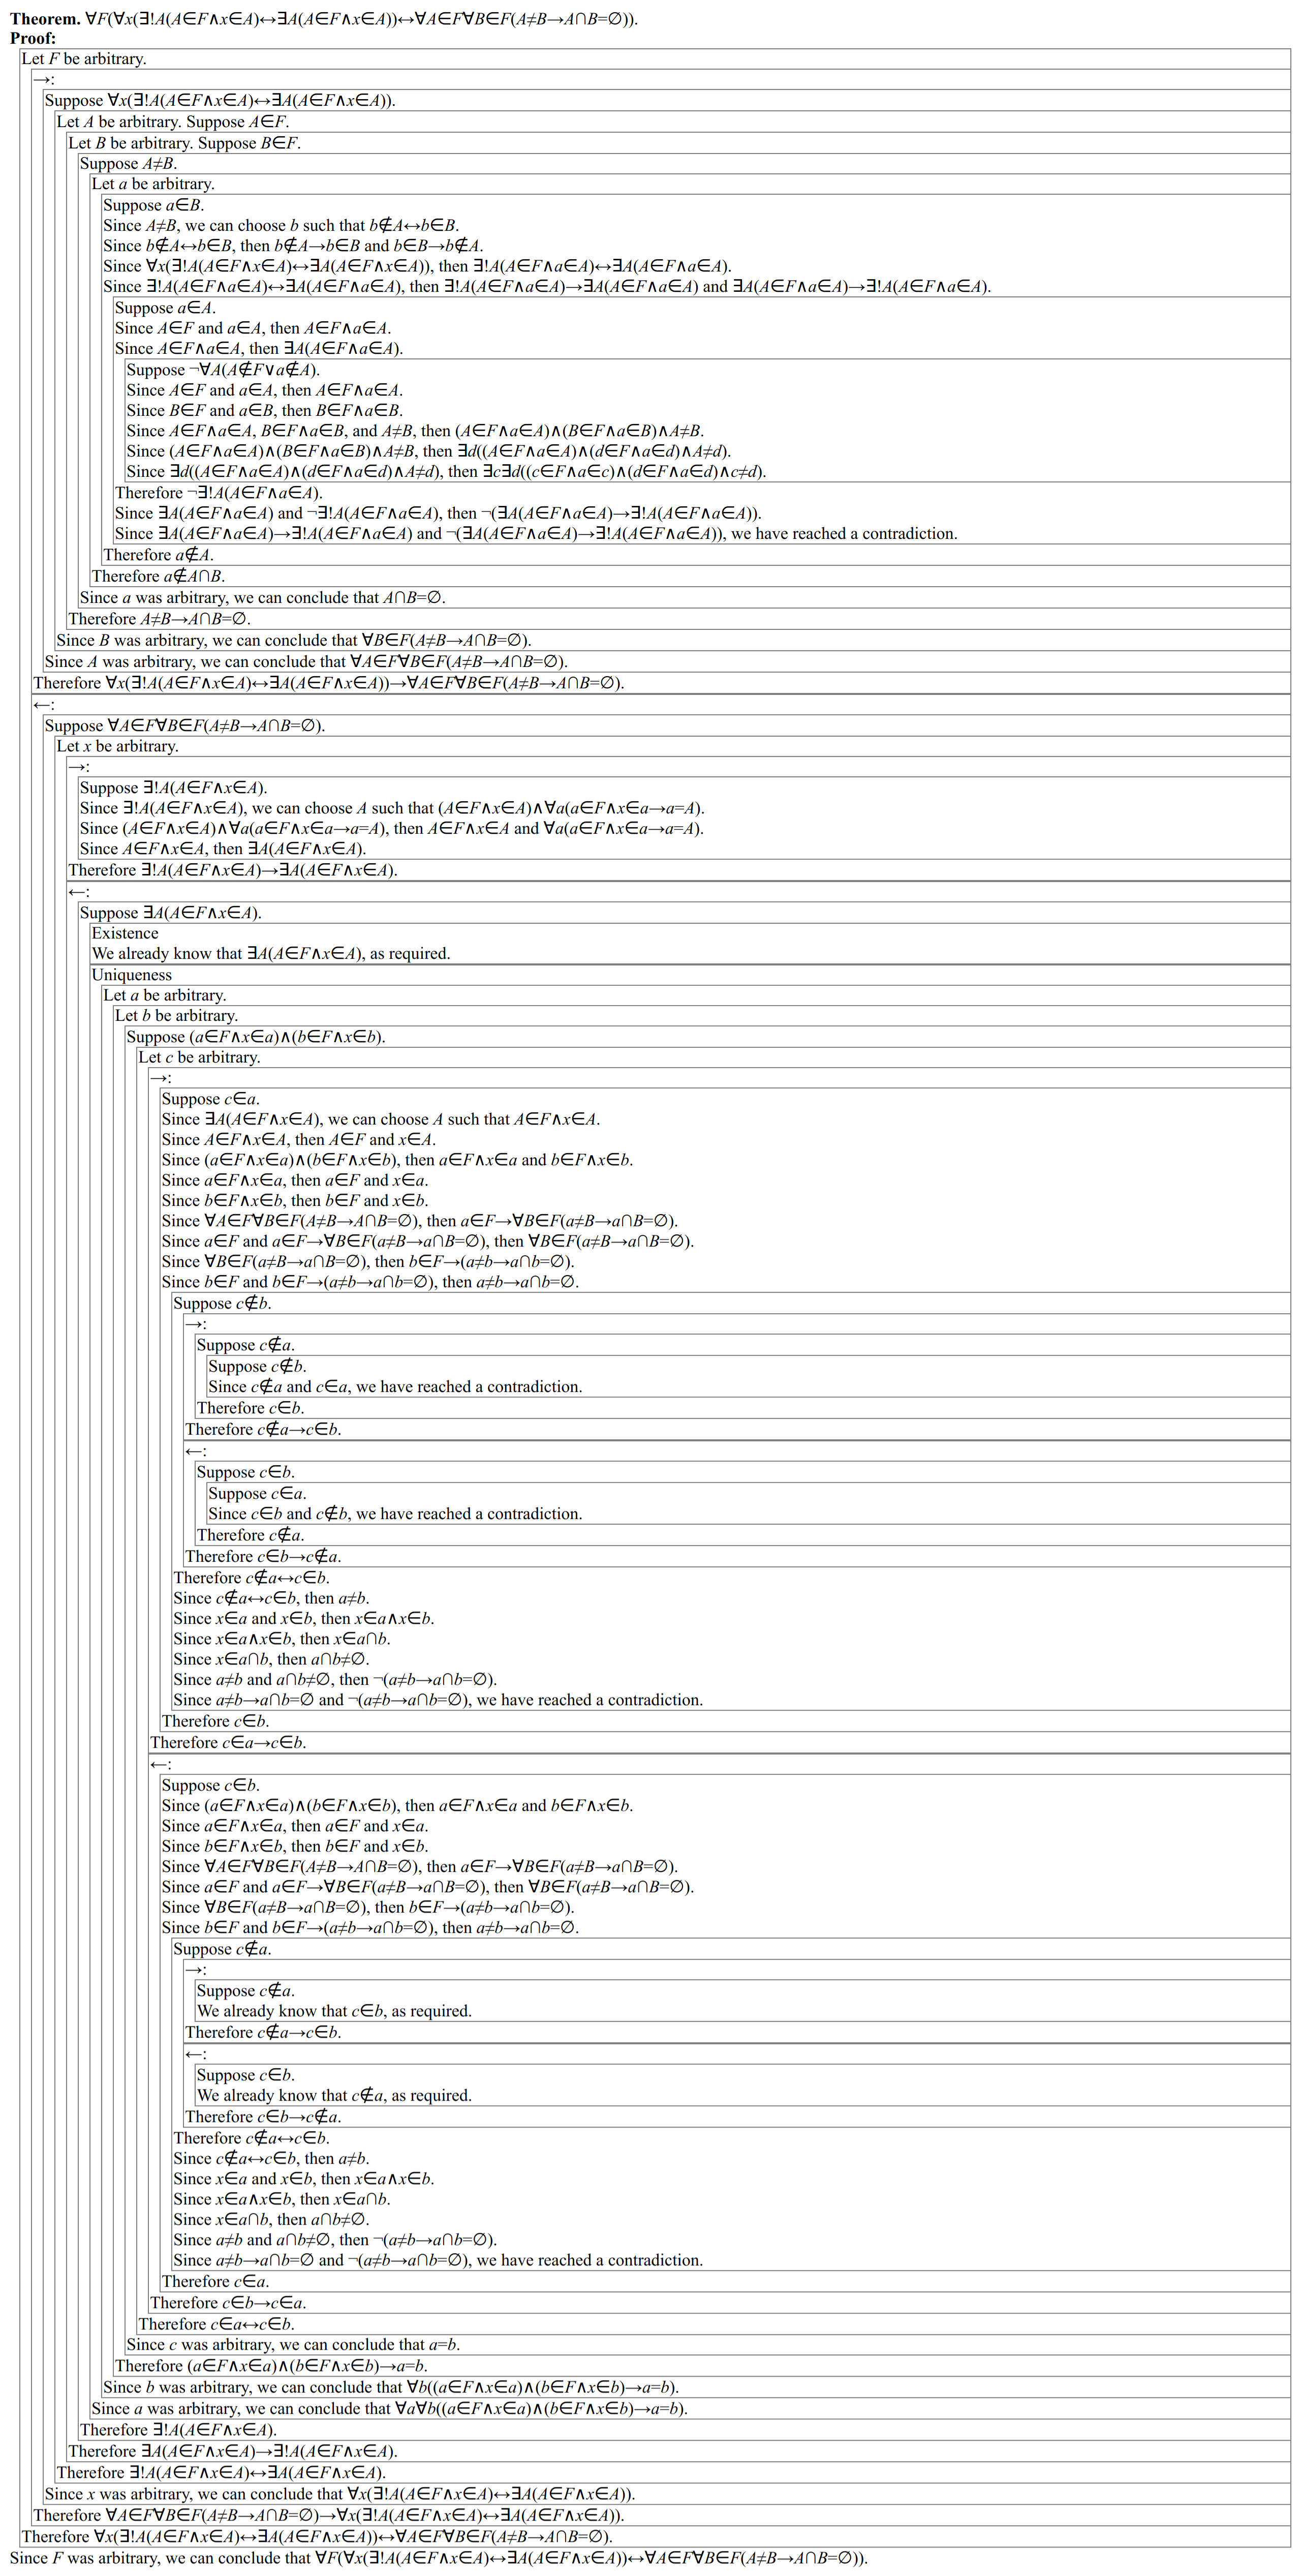
\includegraphics[width=\textwidth,height=\textheight,keepaspectratio]{3_6_5_2}

\vspace{30pt}

$^{\textit{P}}_{\, \textit{D}}$ *6. Let U be any set.

\hspace{12pt}(a) Prove that there is a unique $A \in \mathcal{P} (U)$ such that for every $B \in \mathcal{P} (U)$, $A \cup B = B$.

\hspace{12pt}(b) Prove that there is a unique $A \in \mathcal{P} (U)$ such that for every $B \in \mathcal{P} (U)$, $A \cup B = A$.

\vspace{30pt}

(a)

\textbf{3.6.6.1.pd}
\vspace{10pt}

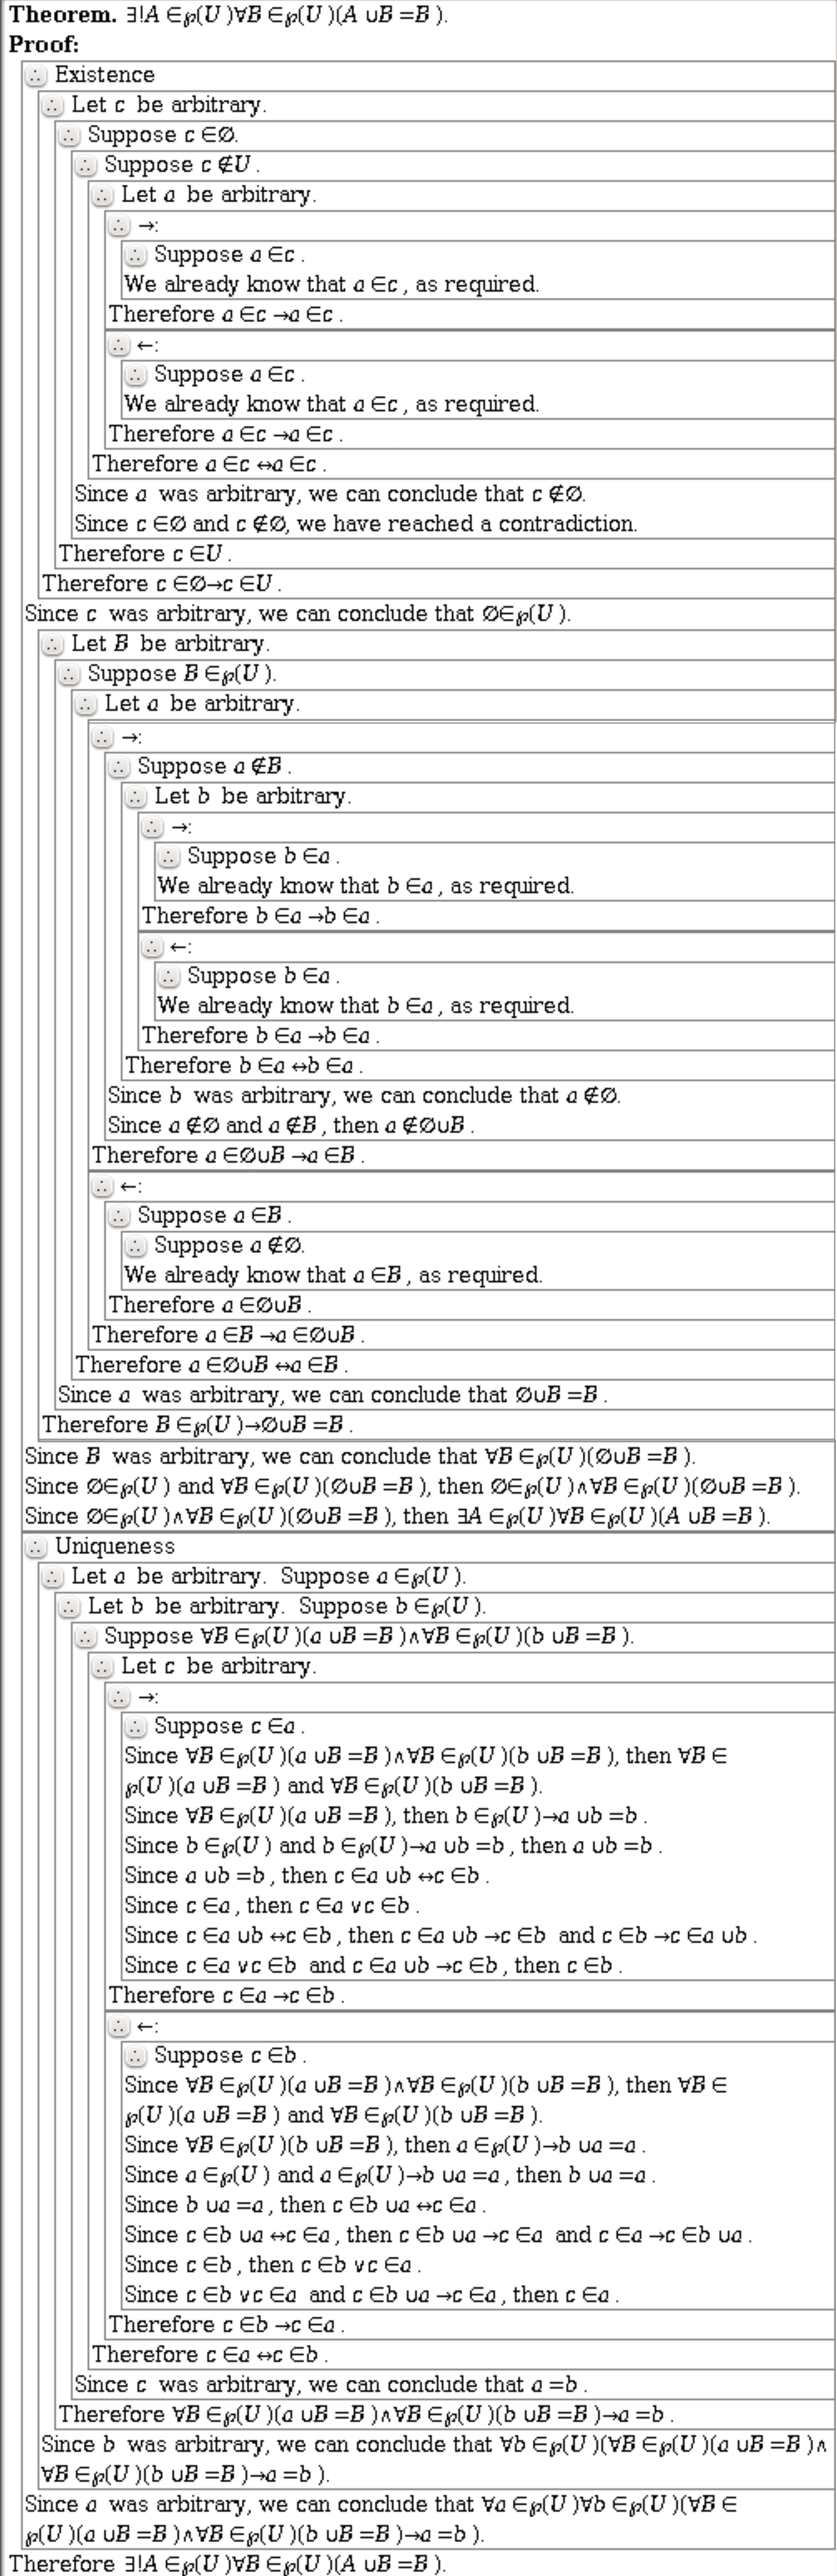
\includegraphics[scale=0.10]{3_6_6_1}

\vspace{30pt}

(b)

\textbf{3.6.6.2.pd}
\vspace{10pt}

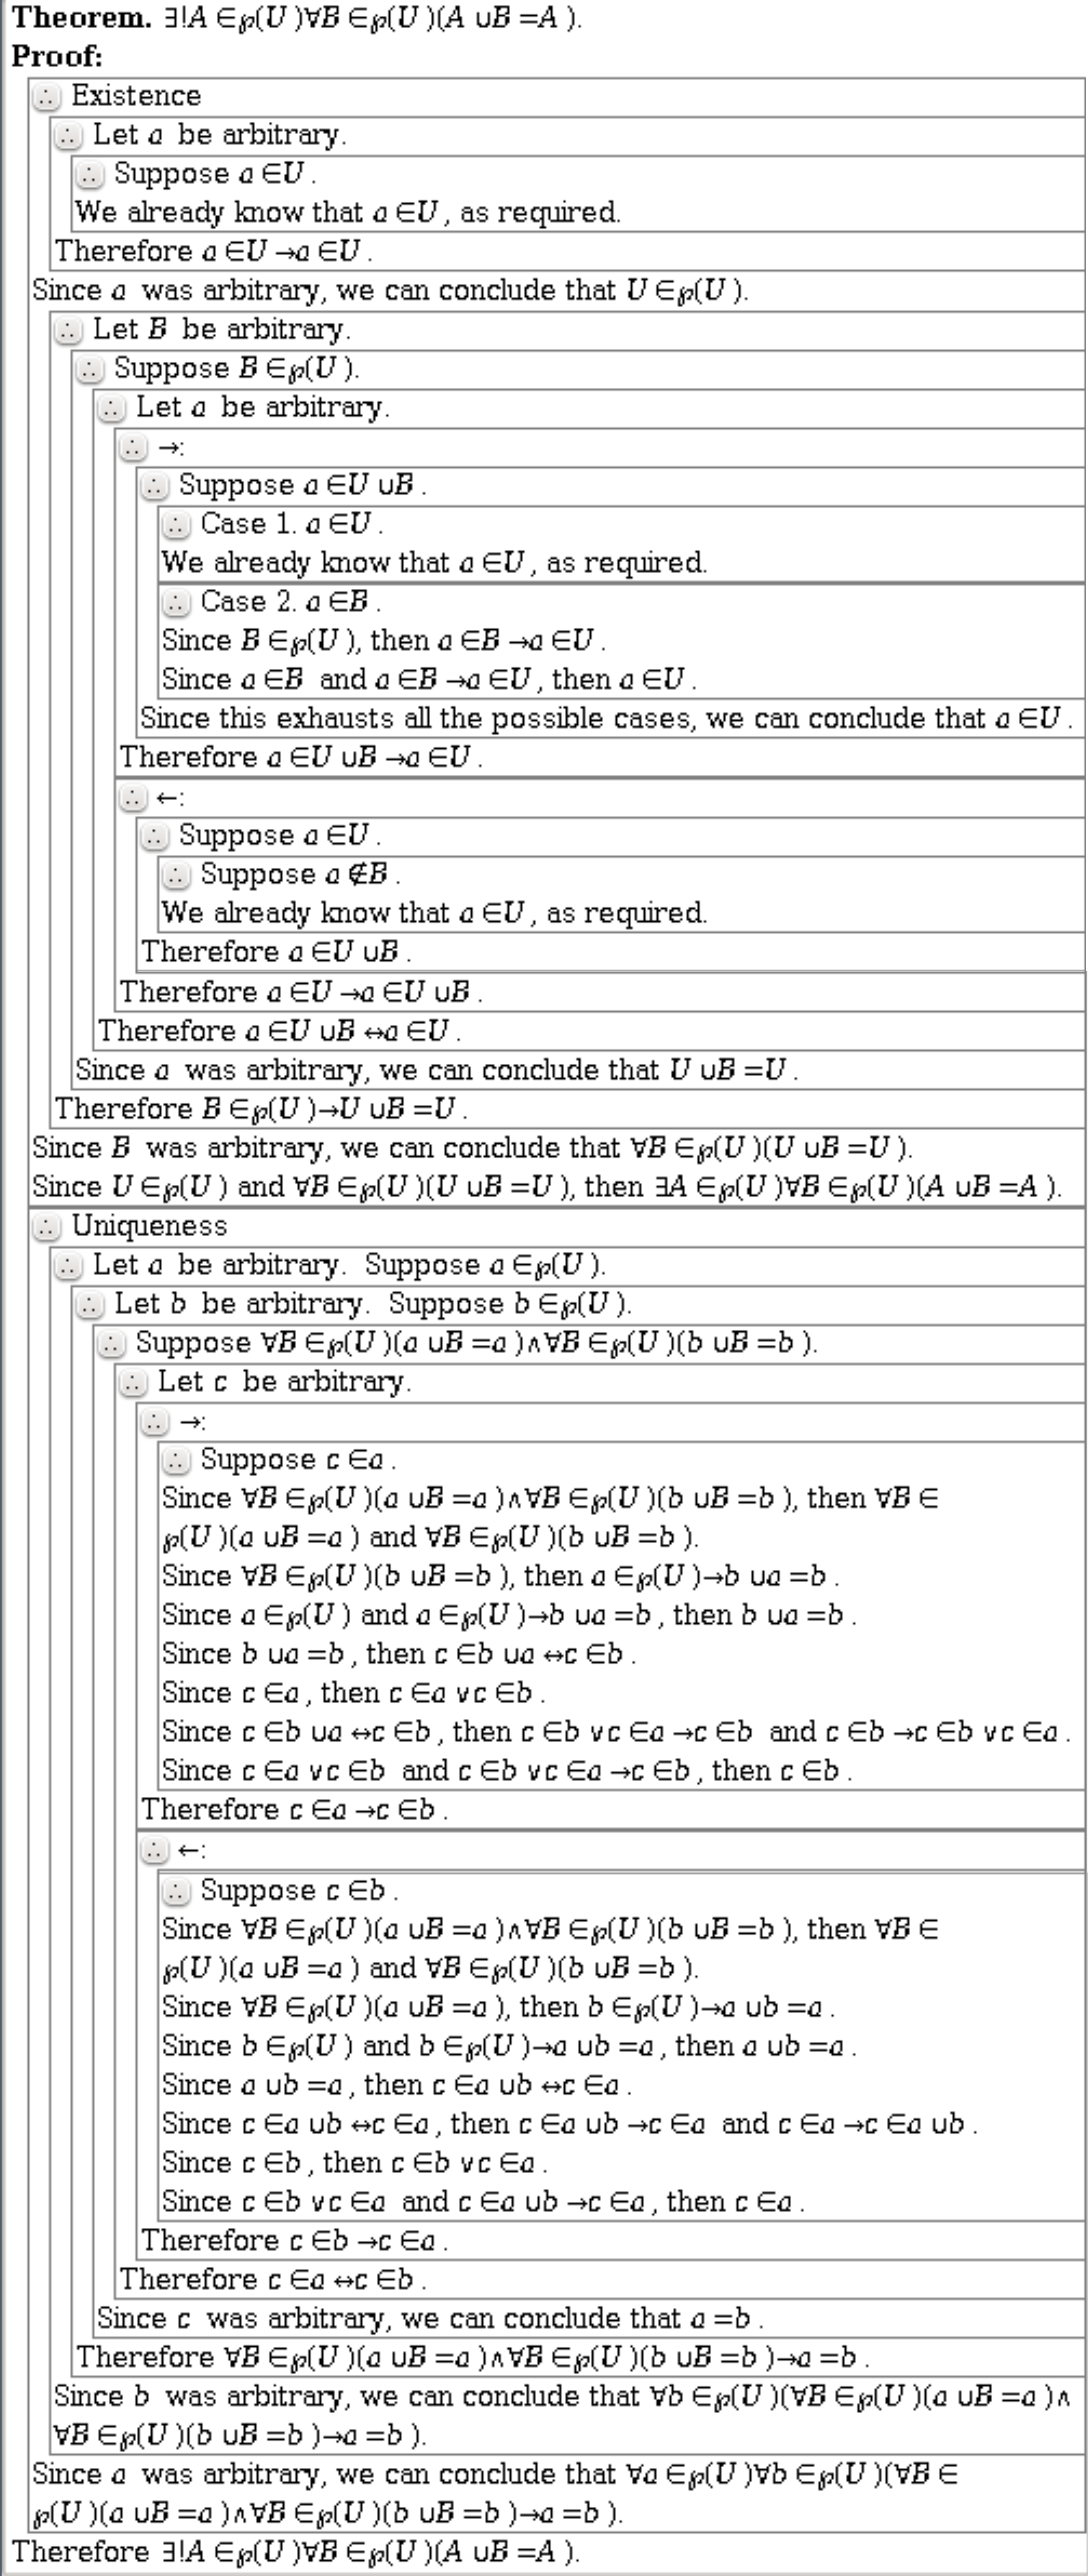
\includegraphics[scale=0.10]{3_6_6_2}

\vspace{30pt}

$^{\textit{P}}_{\, \textit{D}}$ 7. Let U be any set.

\hspace{12pt}(a) Prove that there is a unique $A \in \mathcal{P} (U)$ such that for every $B \in \mathcal{P} (U)$, $A \cap B = B$.

\hspace{12pt}(b) Prove that there is a unique $A \in \mathcal{P} (U)$ such that for every $B \in
\mathcal{P} (U)$, $A \cap B = A$.

\vspace{30pt}

(a)

\textbf{3.6.7.1.pd}
\vspace{10pt}

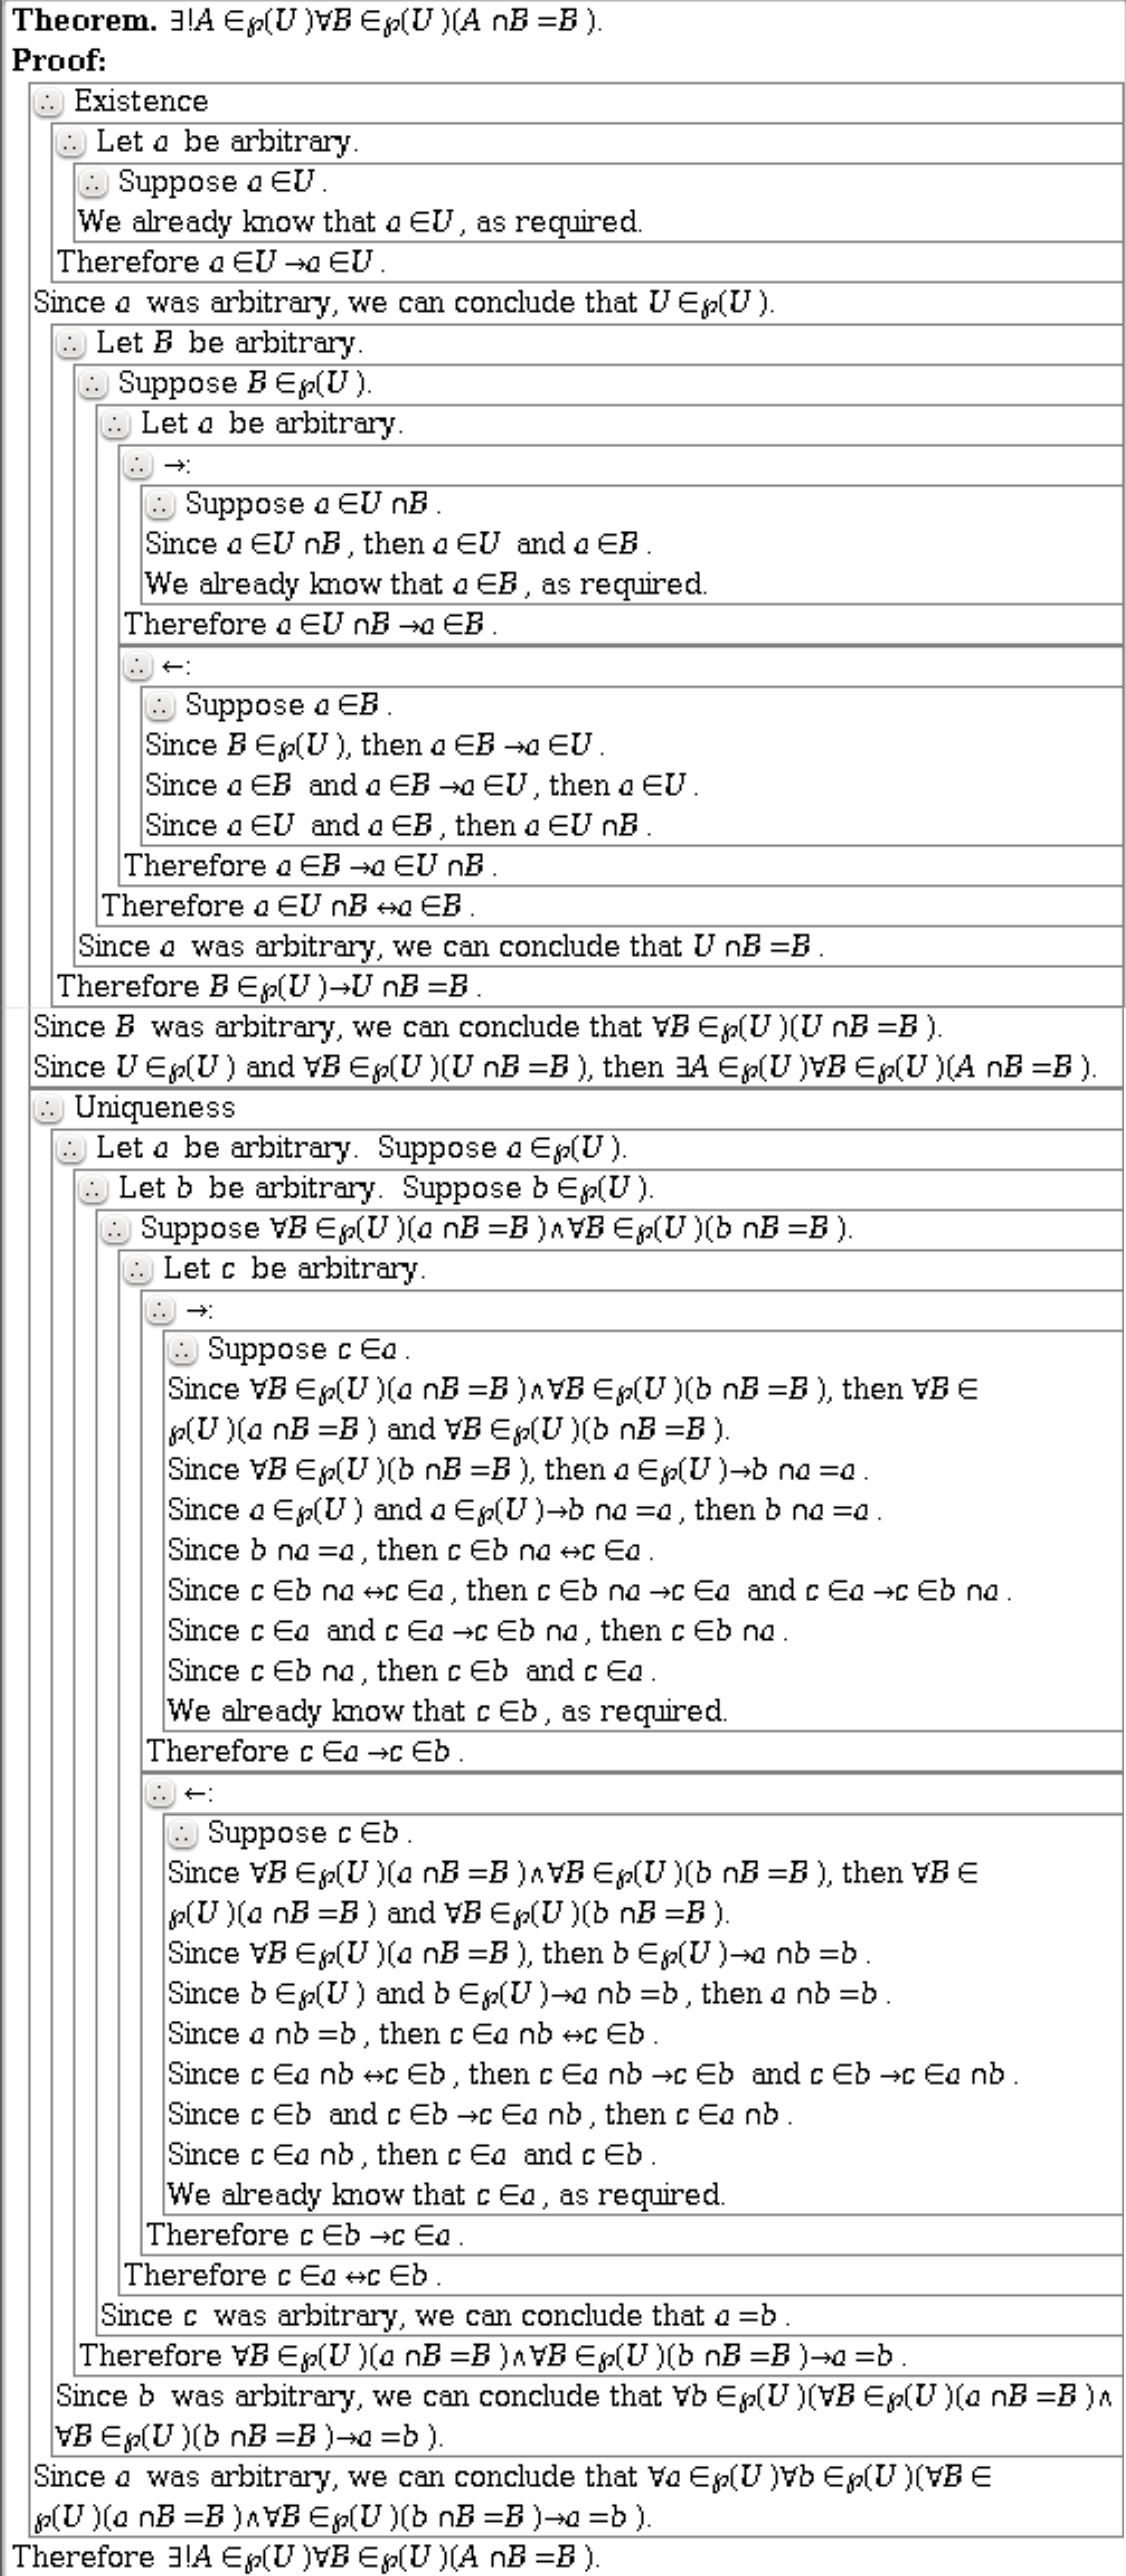
\includegraphics[scale=0.12]{3_6_7_1}

\vspace{30pt}

(b)

\textbf{3.6.7.2.pd}
\vspace{10pt}

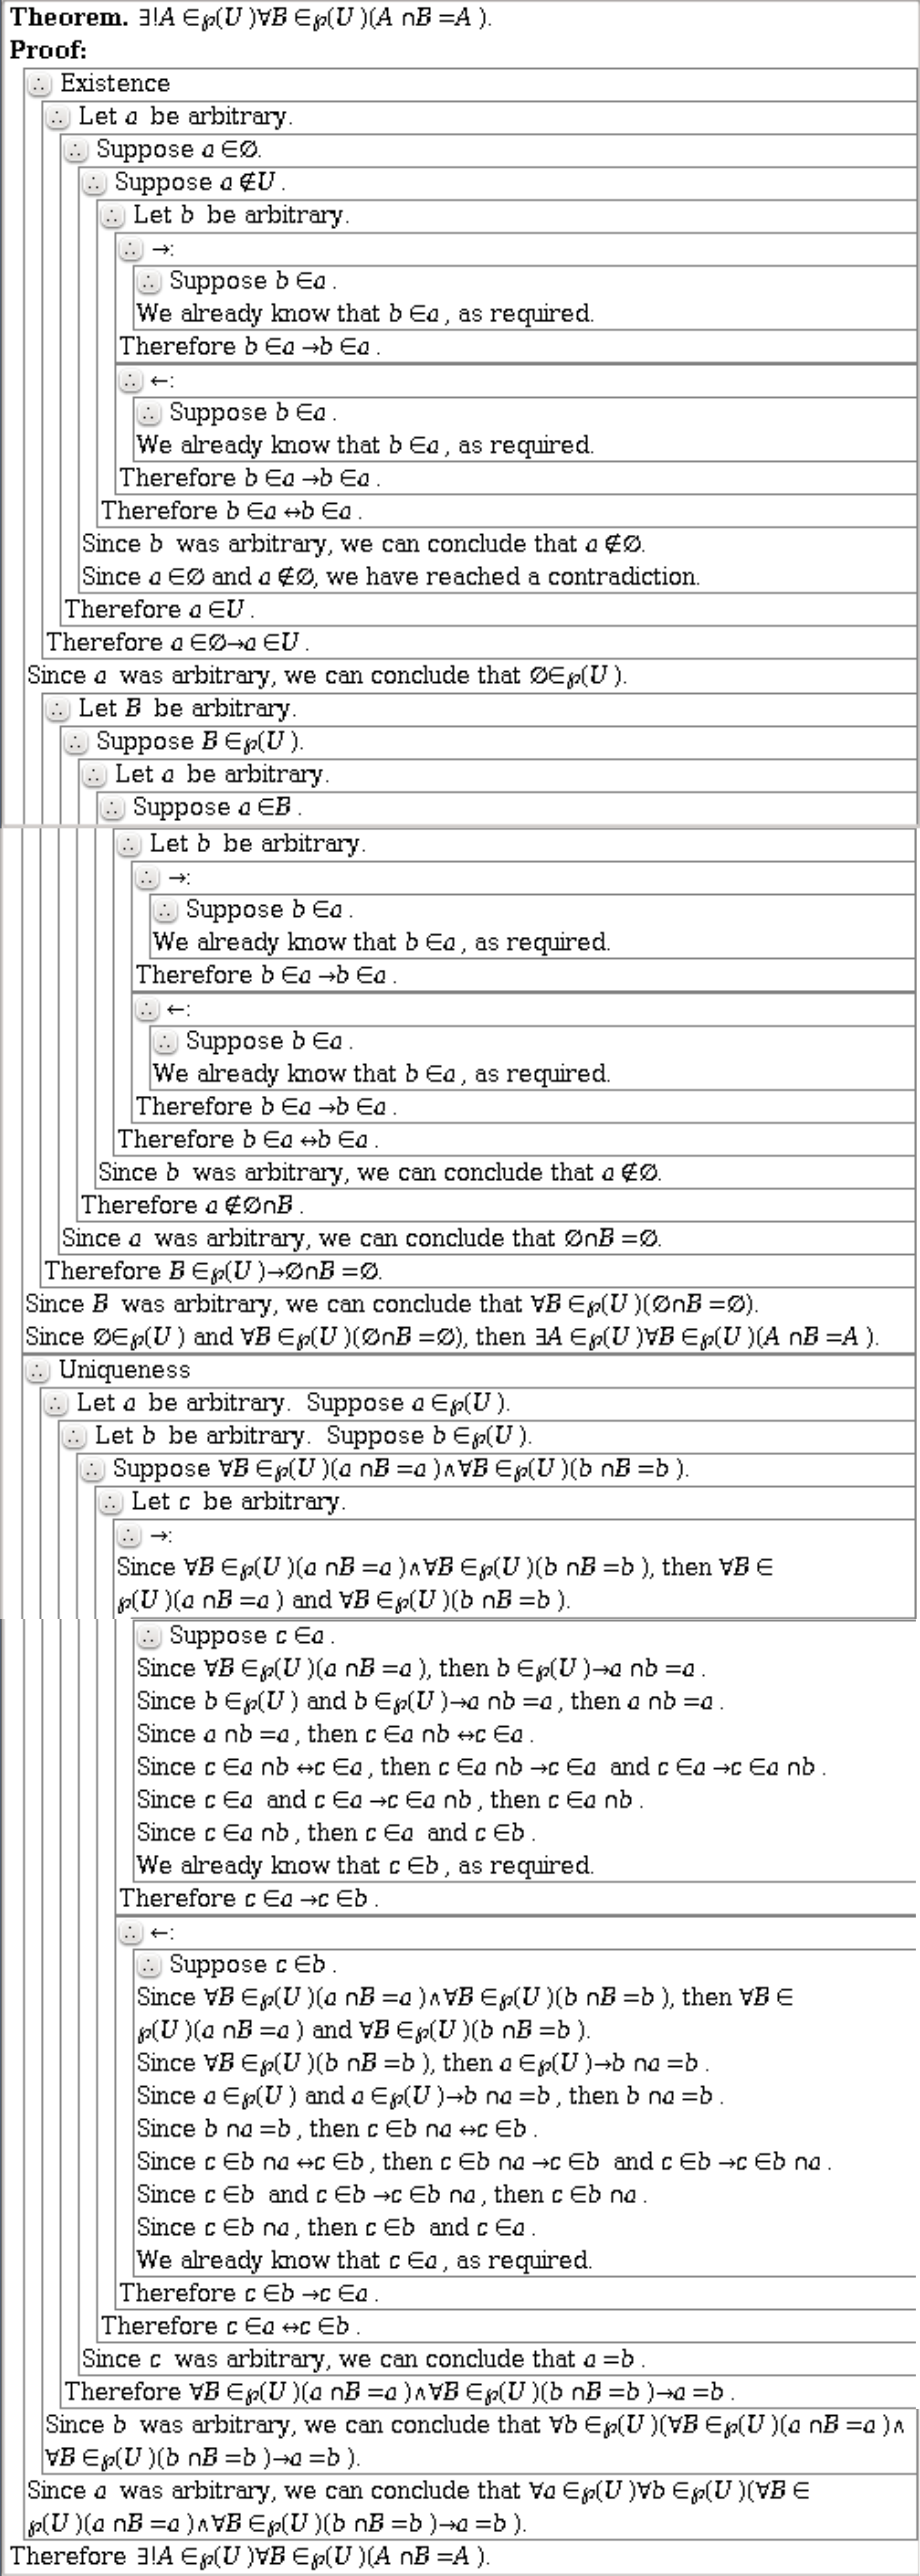
\includegraphics[scale=0.12]{3_6_7_2}

\vspace{30pt}

$^{\textit{P}}_{\, \textit{D}}$ 8. Let U be any set.

\hspace{12pt}(a) Prove that for every $A \in \mathcal{P} (U)$ there is a unique $B \in \mathcal{P} (U)$ such
that for every $C \in \mathcal{P} (U)$, $C \setminus A = C \cap B$.

\hspace{12pt}(b) Prove that for every $A \in \mathcal{P} (U)$ there is a unique $B \in \mathcal{P} (U)$ such
that for every $C \in \mathcal{P} (U)$, $C \cap A = C \setminus B$.

\vspace{30pt}

(a)

\textbf{3.6.8.1.pd}
\vspace{10pt}

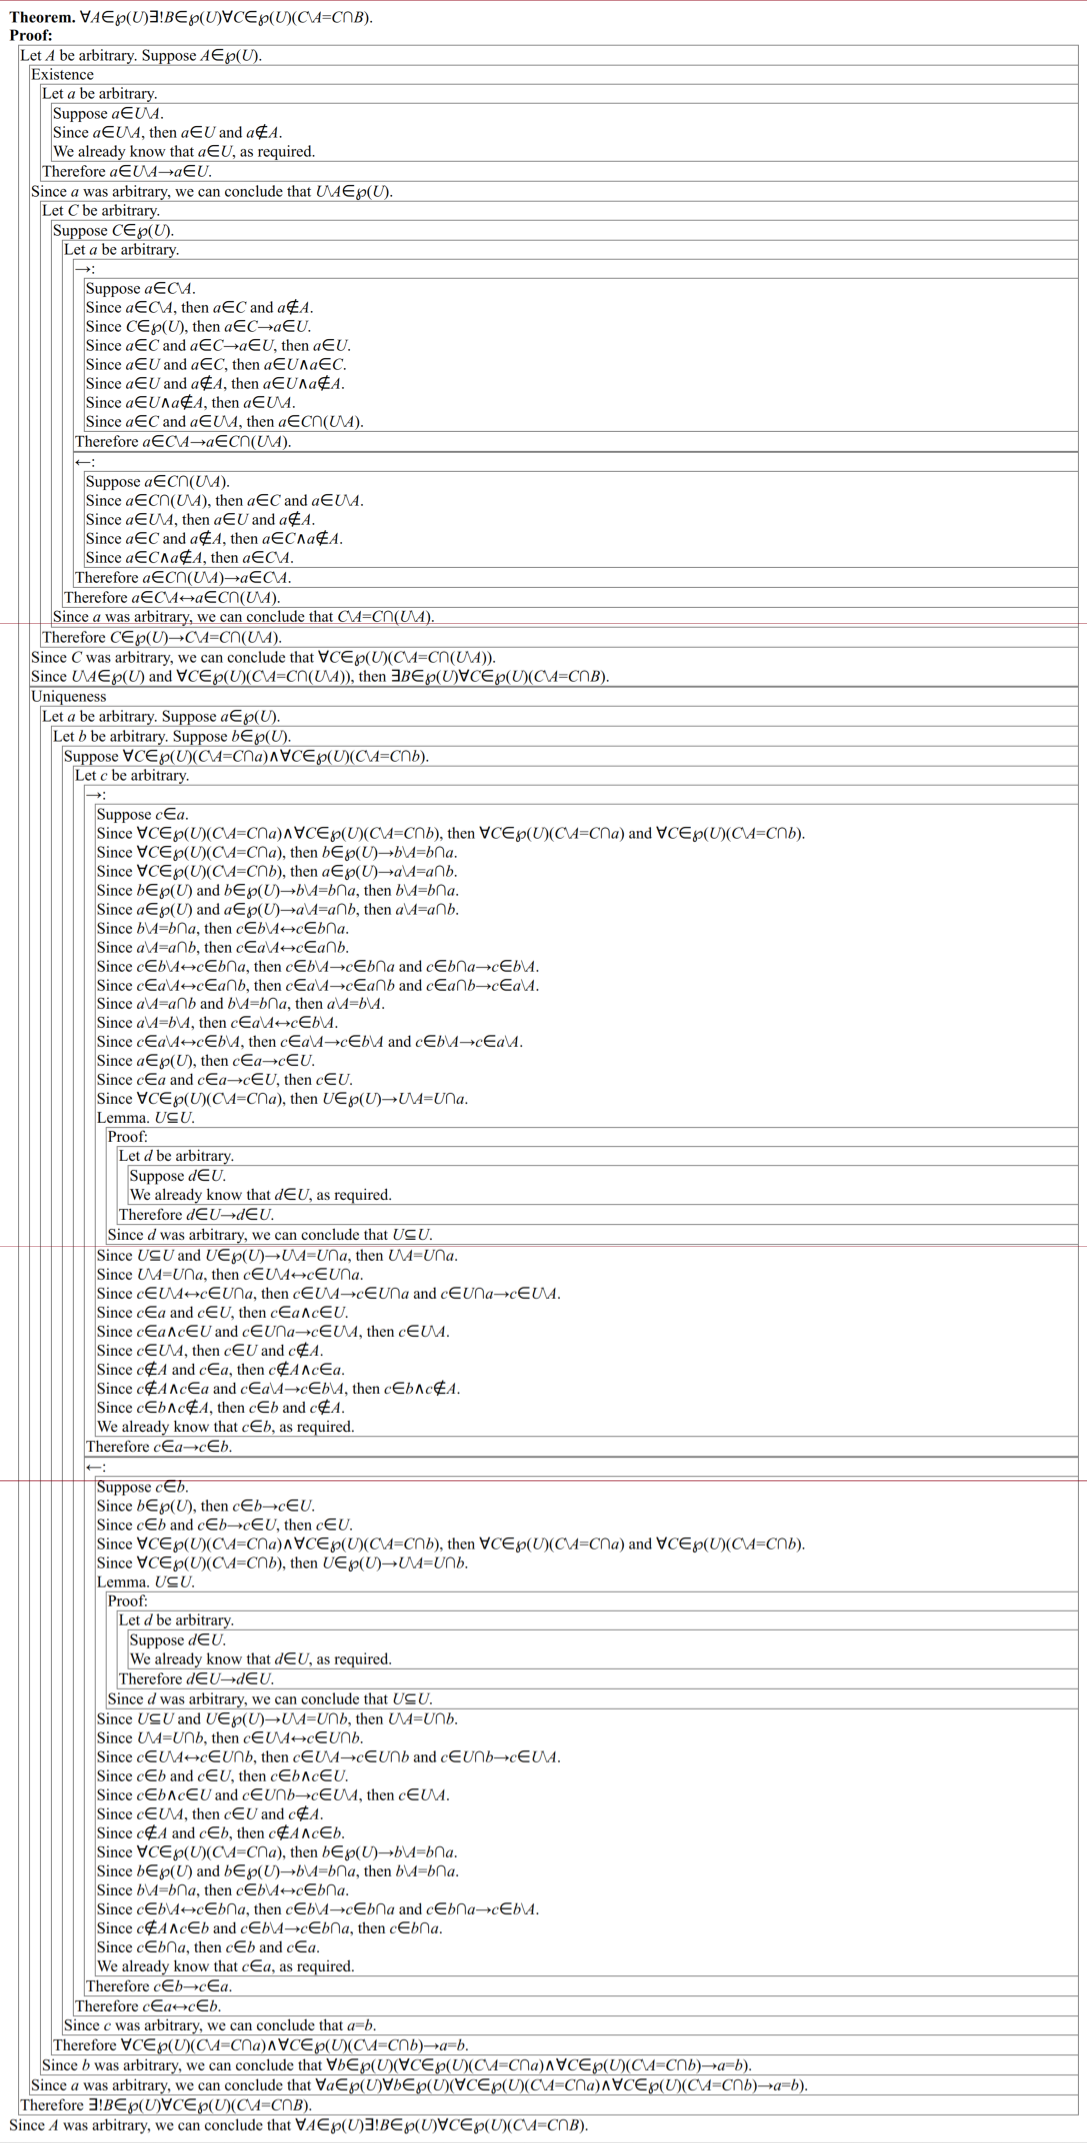
\includegraphics[scale=0.25]{3_6_8_1}

\vspace{30pt}

(b)

\textbf{3.6.8.2.pd}
\vspace{10pt}

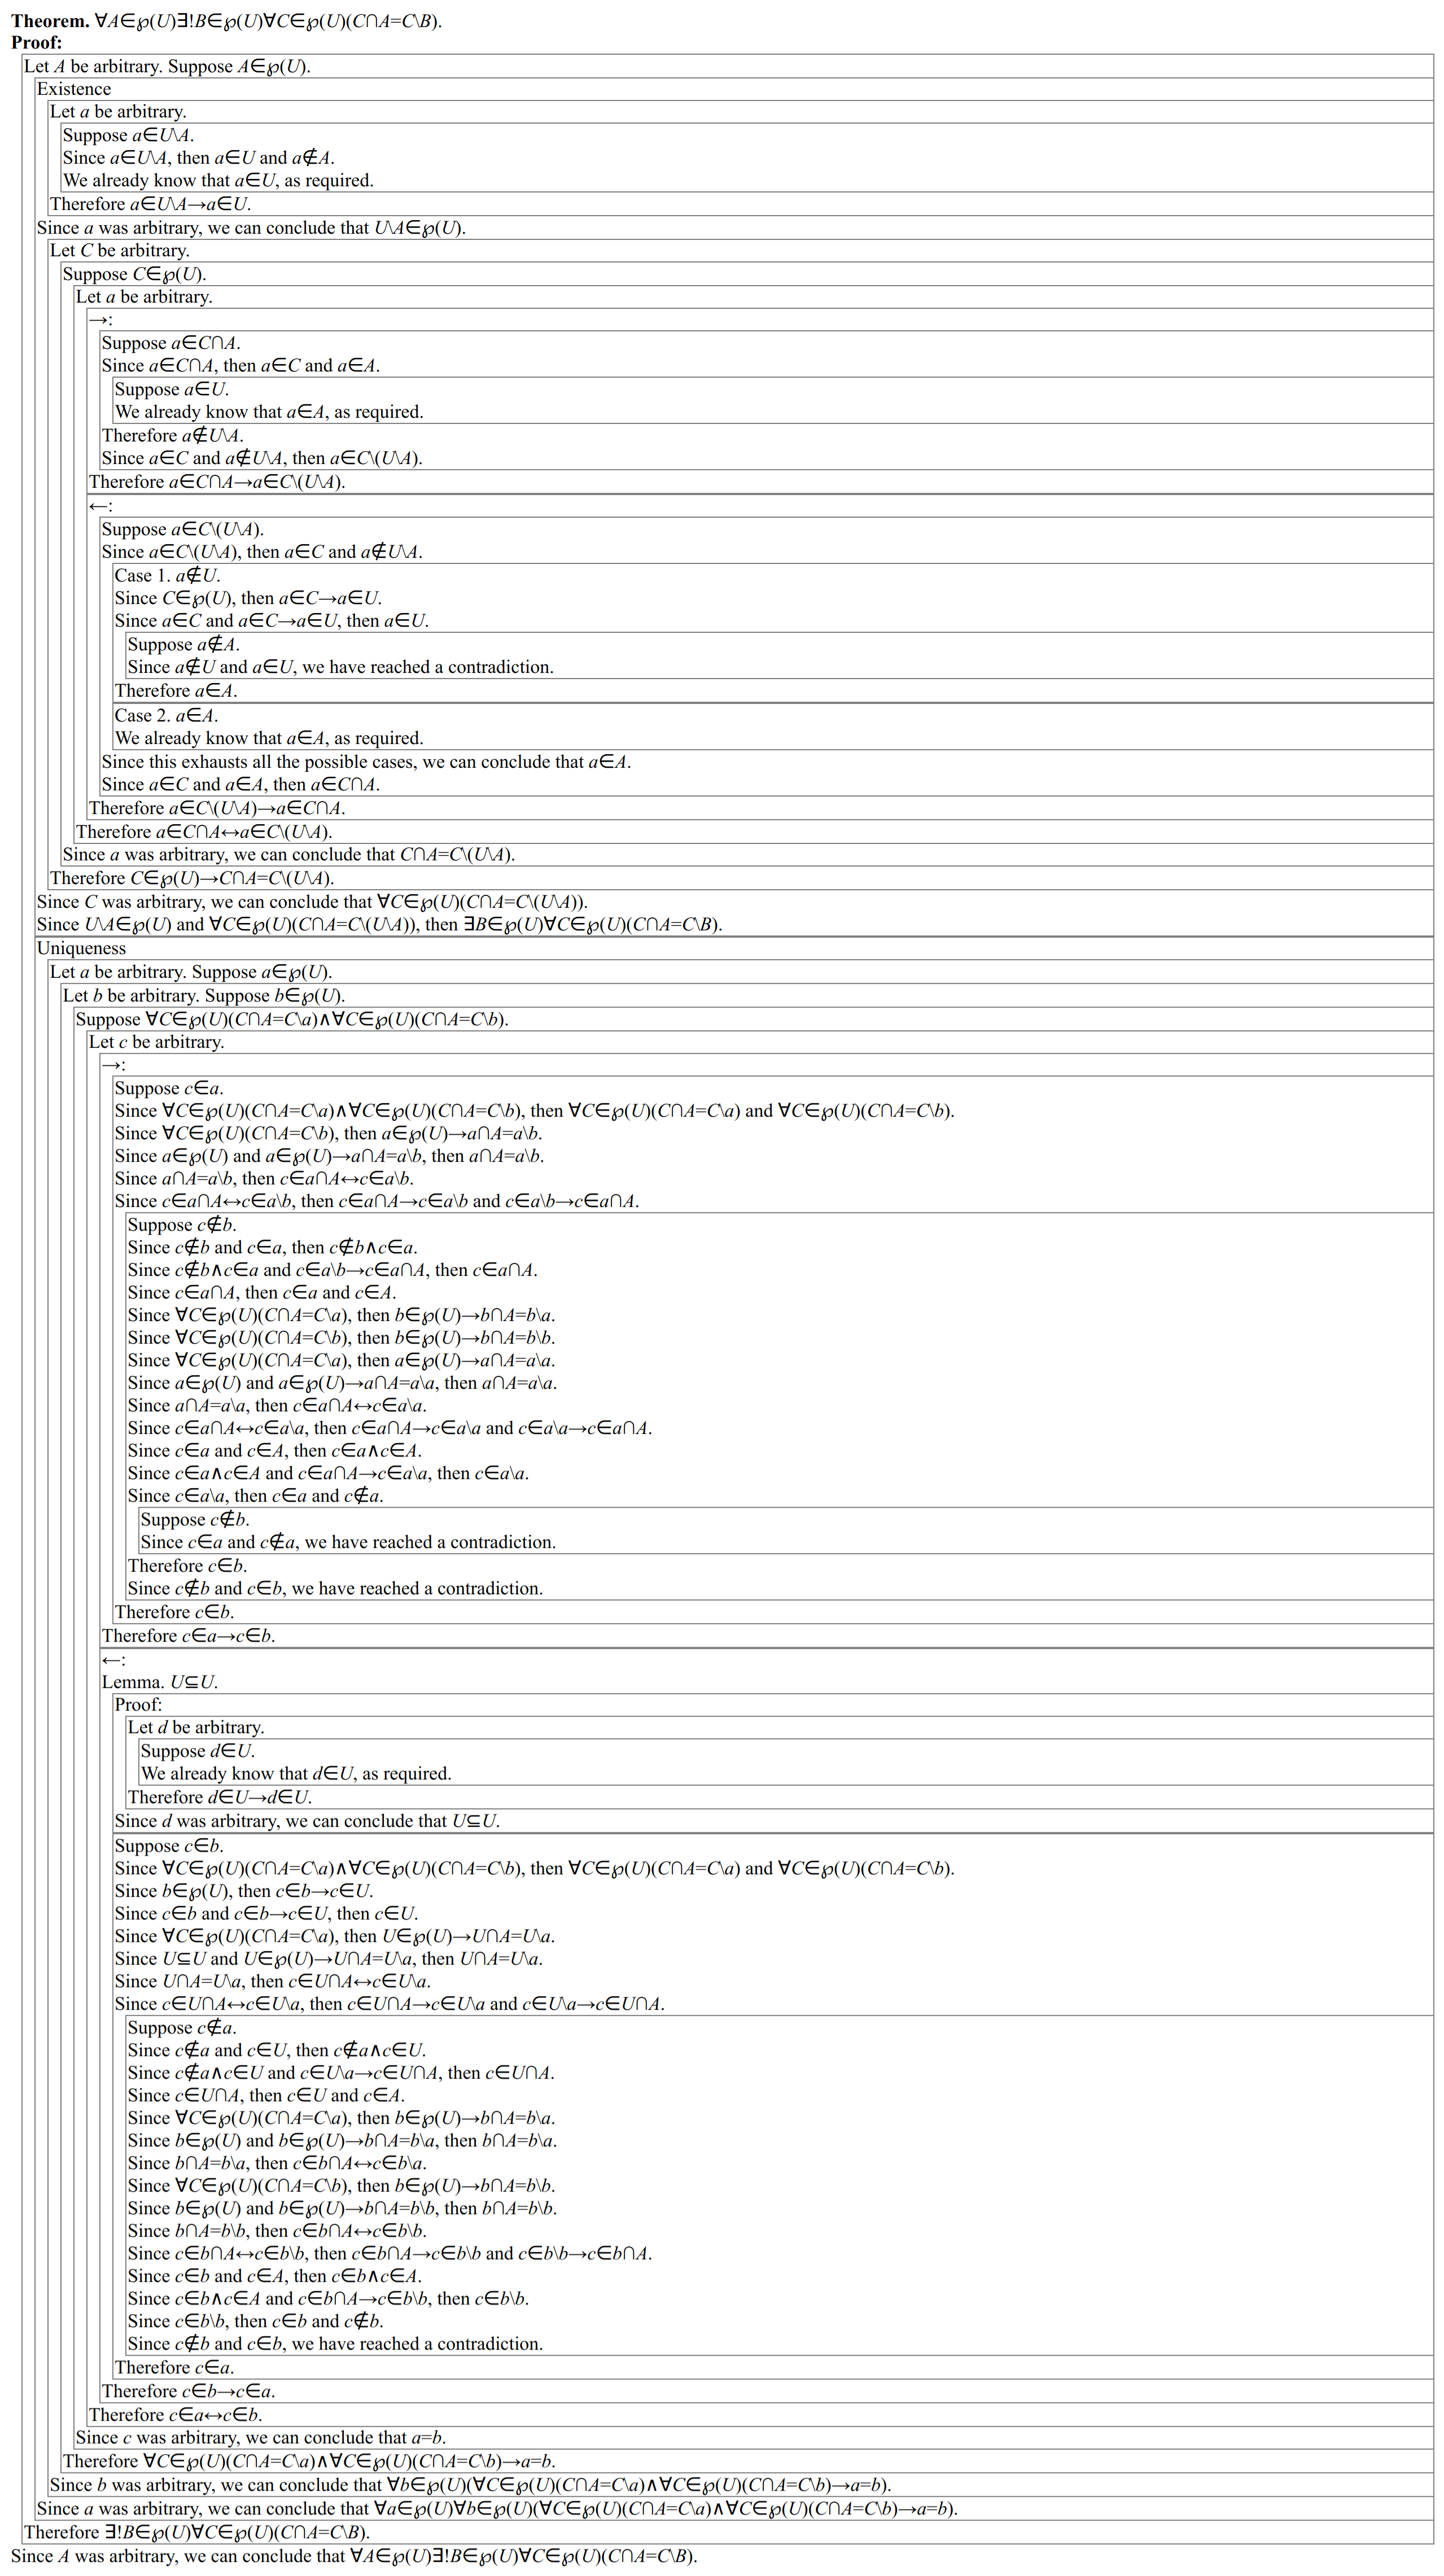
\includegraphics[width=\textwidth,height=\textheight,keepaspectratio]{3_6_8_2}

\vspace{30pt}

$^{\textit{P}}_{\, \textit{D}}$ 9. Recall that you showed in exercise 12 of Section 1.4 that symmetric
difference is associative; in other words, for all sets A, B, and C,
$A \Delta (B \Delta C) = (A \Delta B) \Delta C$. You may also find it useful in this problem
to note that symmetric difference is clearly commutative; in other
words, for all sets A and B, $A \Delta B = B \Delta A$.

\hspace{12pt}(a) Prove that there is a unique identity element for symmetric difference.
In other words, there is a unique set X such that for every set
A, $A \Delta X = A$.

\hspace{12pt}(b) Prove that every set has a unique inverse for the operation of symmetric
difference. In other words, for every set A there is a unique set B
such that $A \Delta B = X$, where X is the identity element from part (a).

\hspace{12pt}(c) Prove that for any sets A and B there is a unique set C such that
$A \Delta C = B$.

\hspace{12pt}(d) Prove that for every set A there is a unique set $B \subseteq A$ such that for
every set $C \subseteq A$, $B \Delta C = A \setminus C$.

\vspace{30pt}

(a)

\textbf{3.6.9.1.pd}
\vspace{10pt}

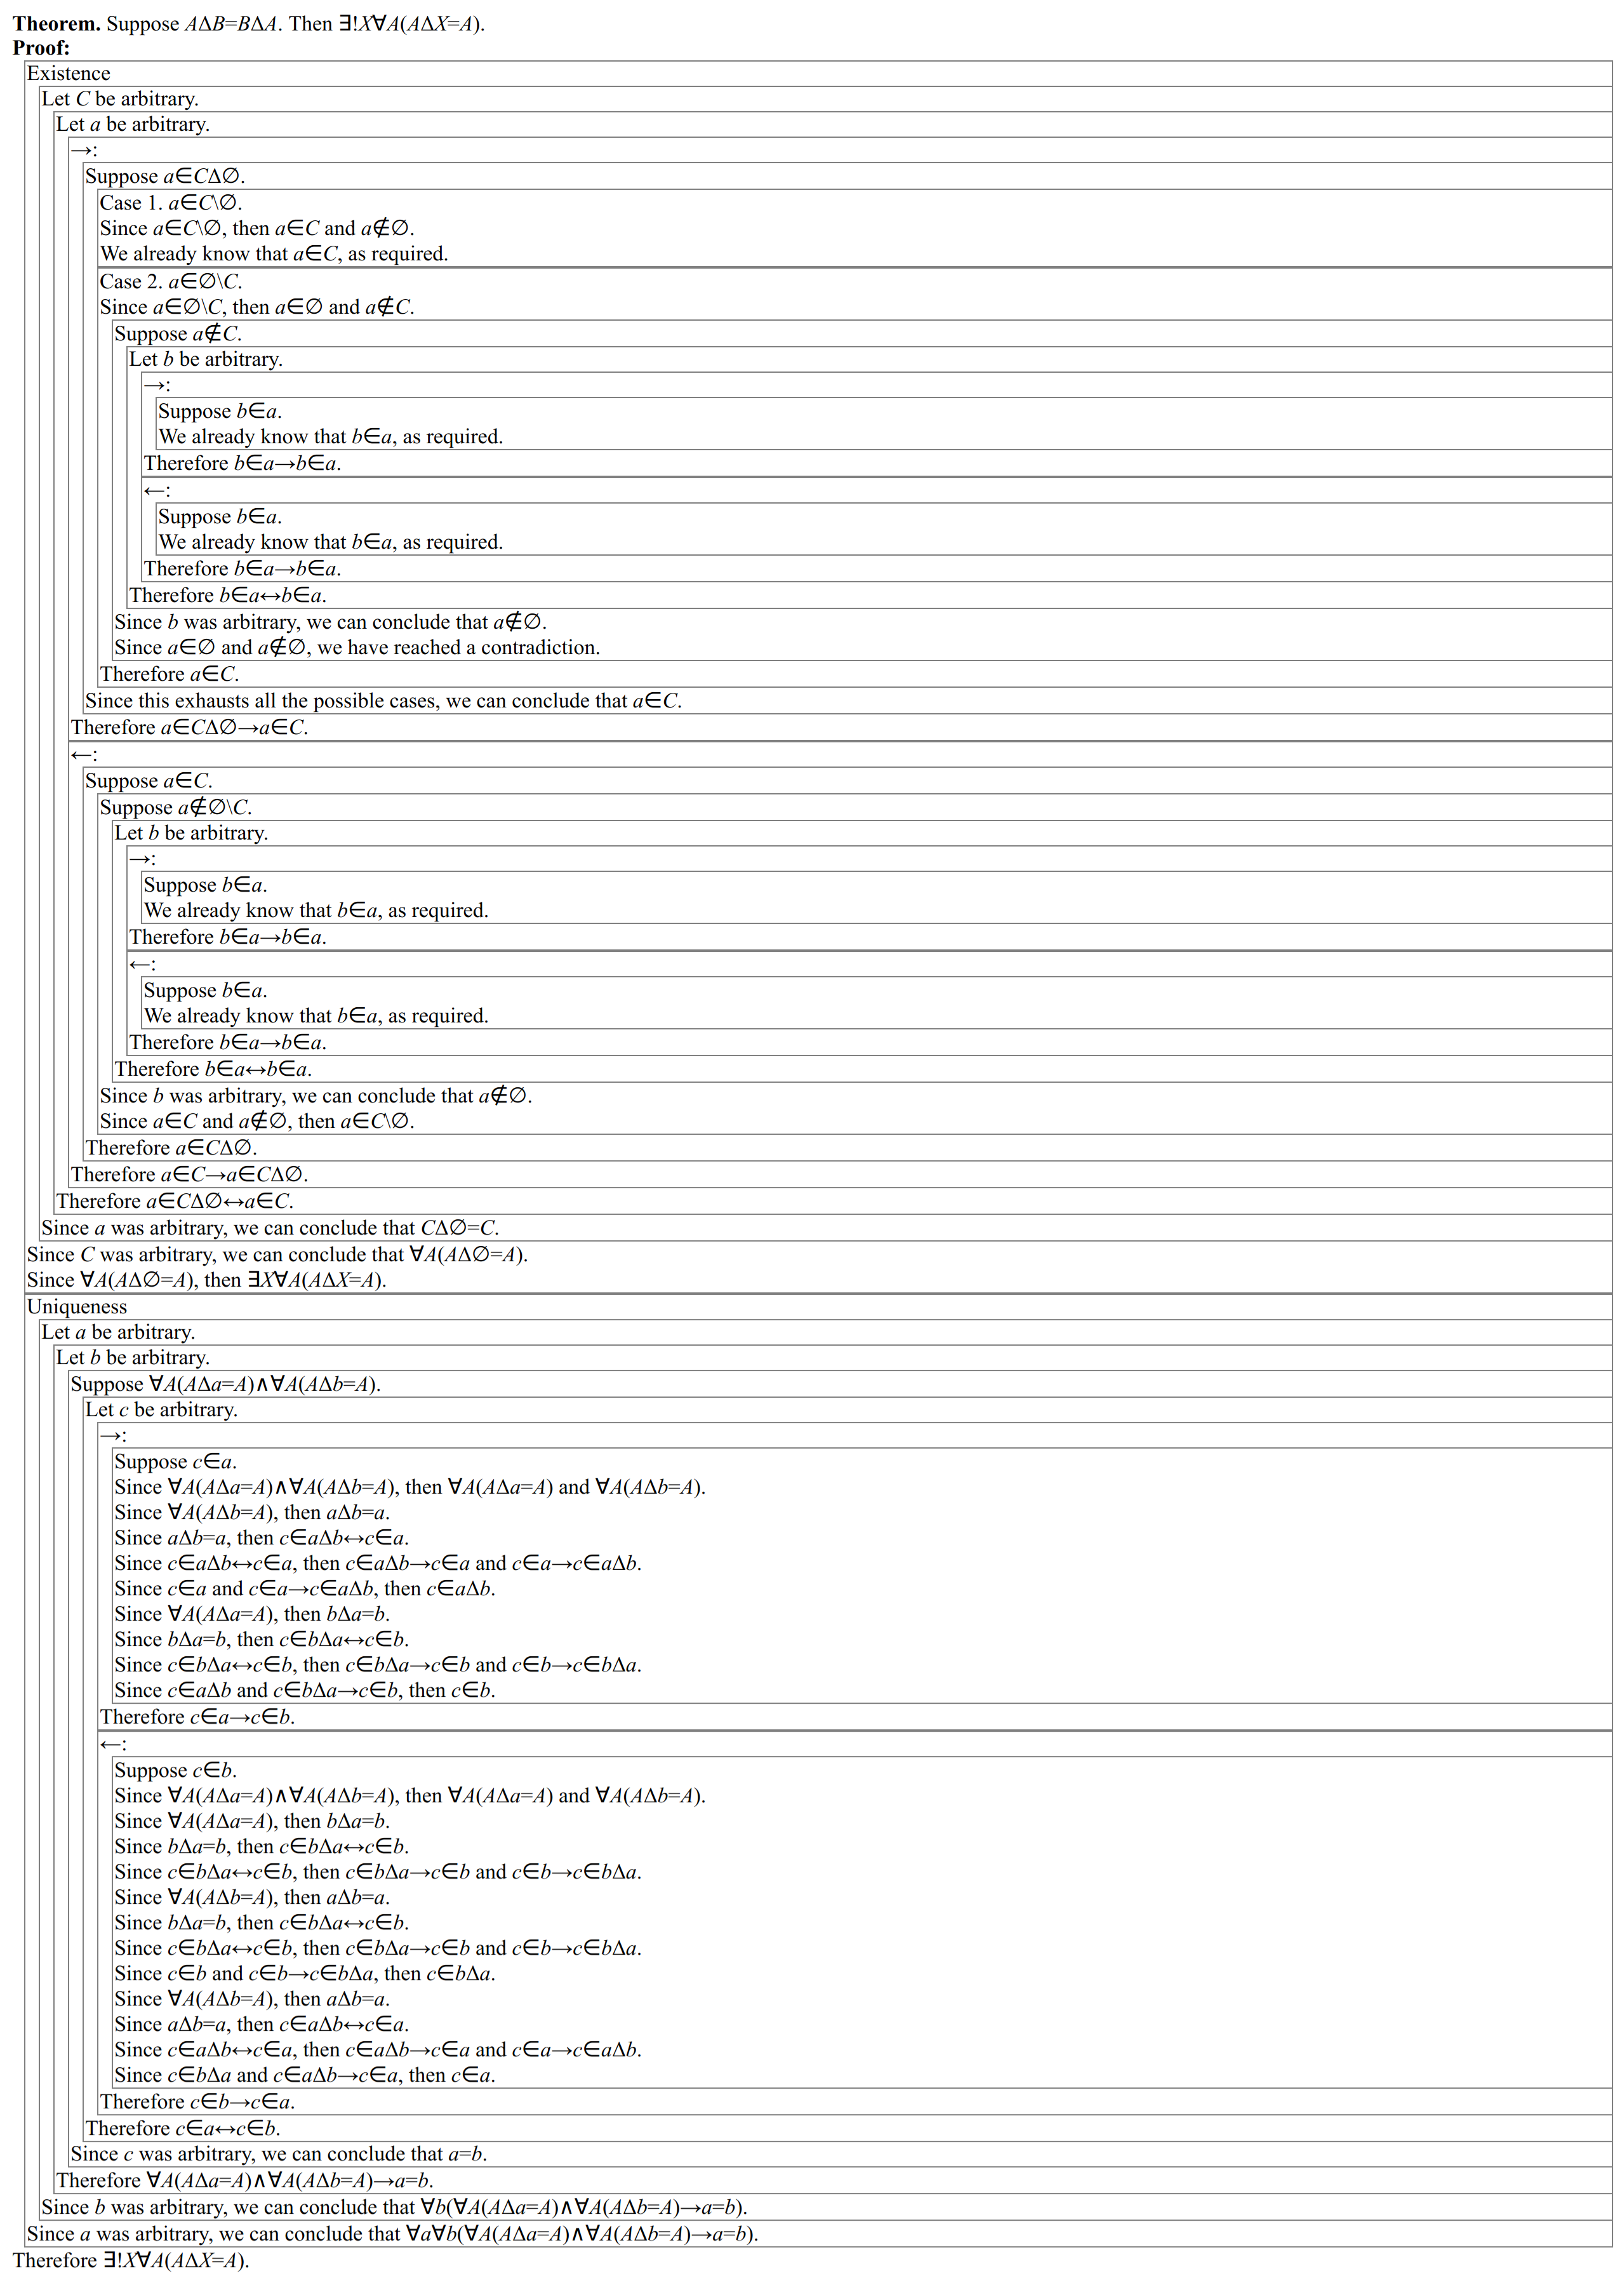
\includegraphics[width=\textwidth,height=\textheight,keepaspectratio]{3_6_9_1}

\vspace{30pt}

(b)

\textbf{3.6.9.2.pd}
\vspace{10pt}

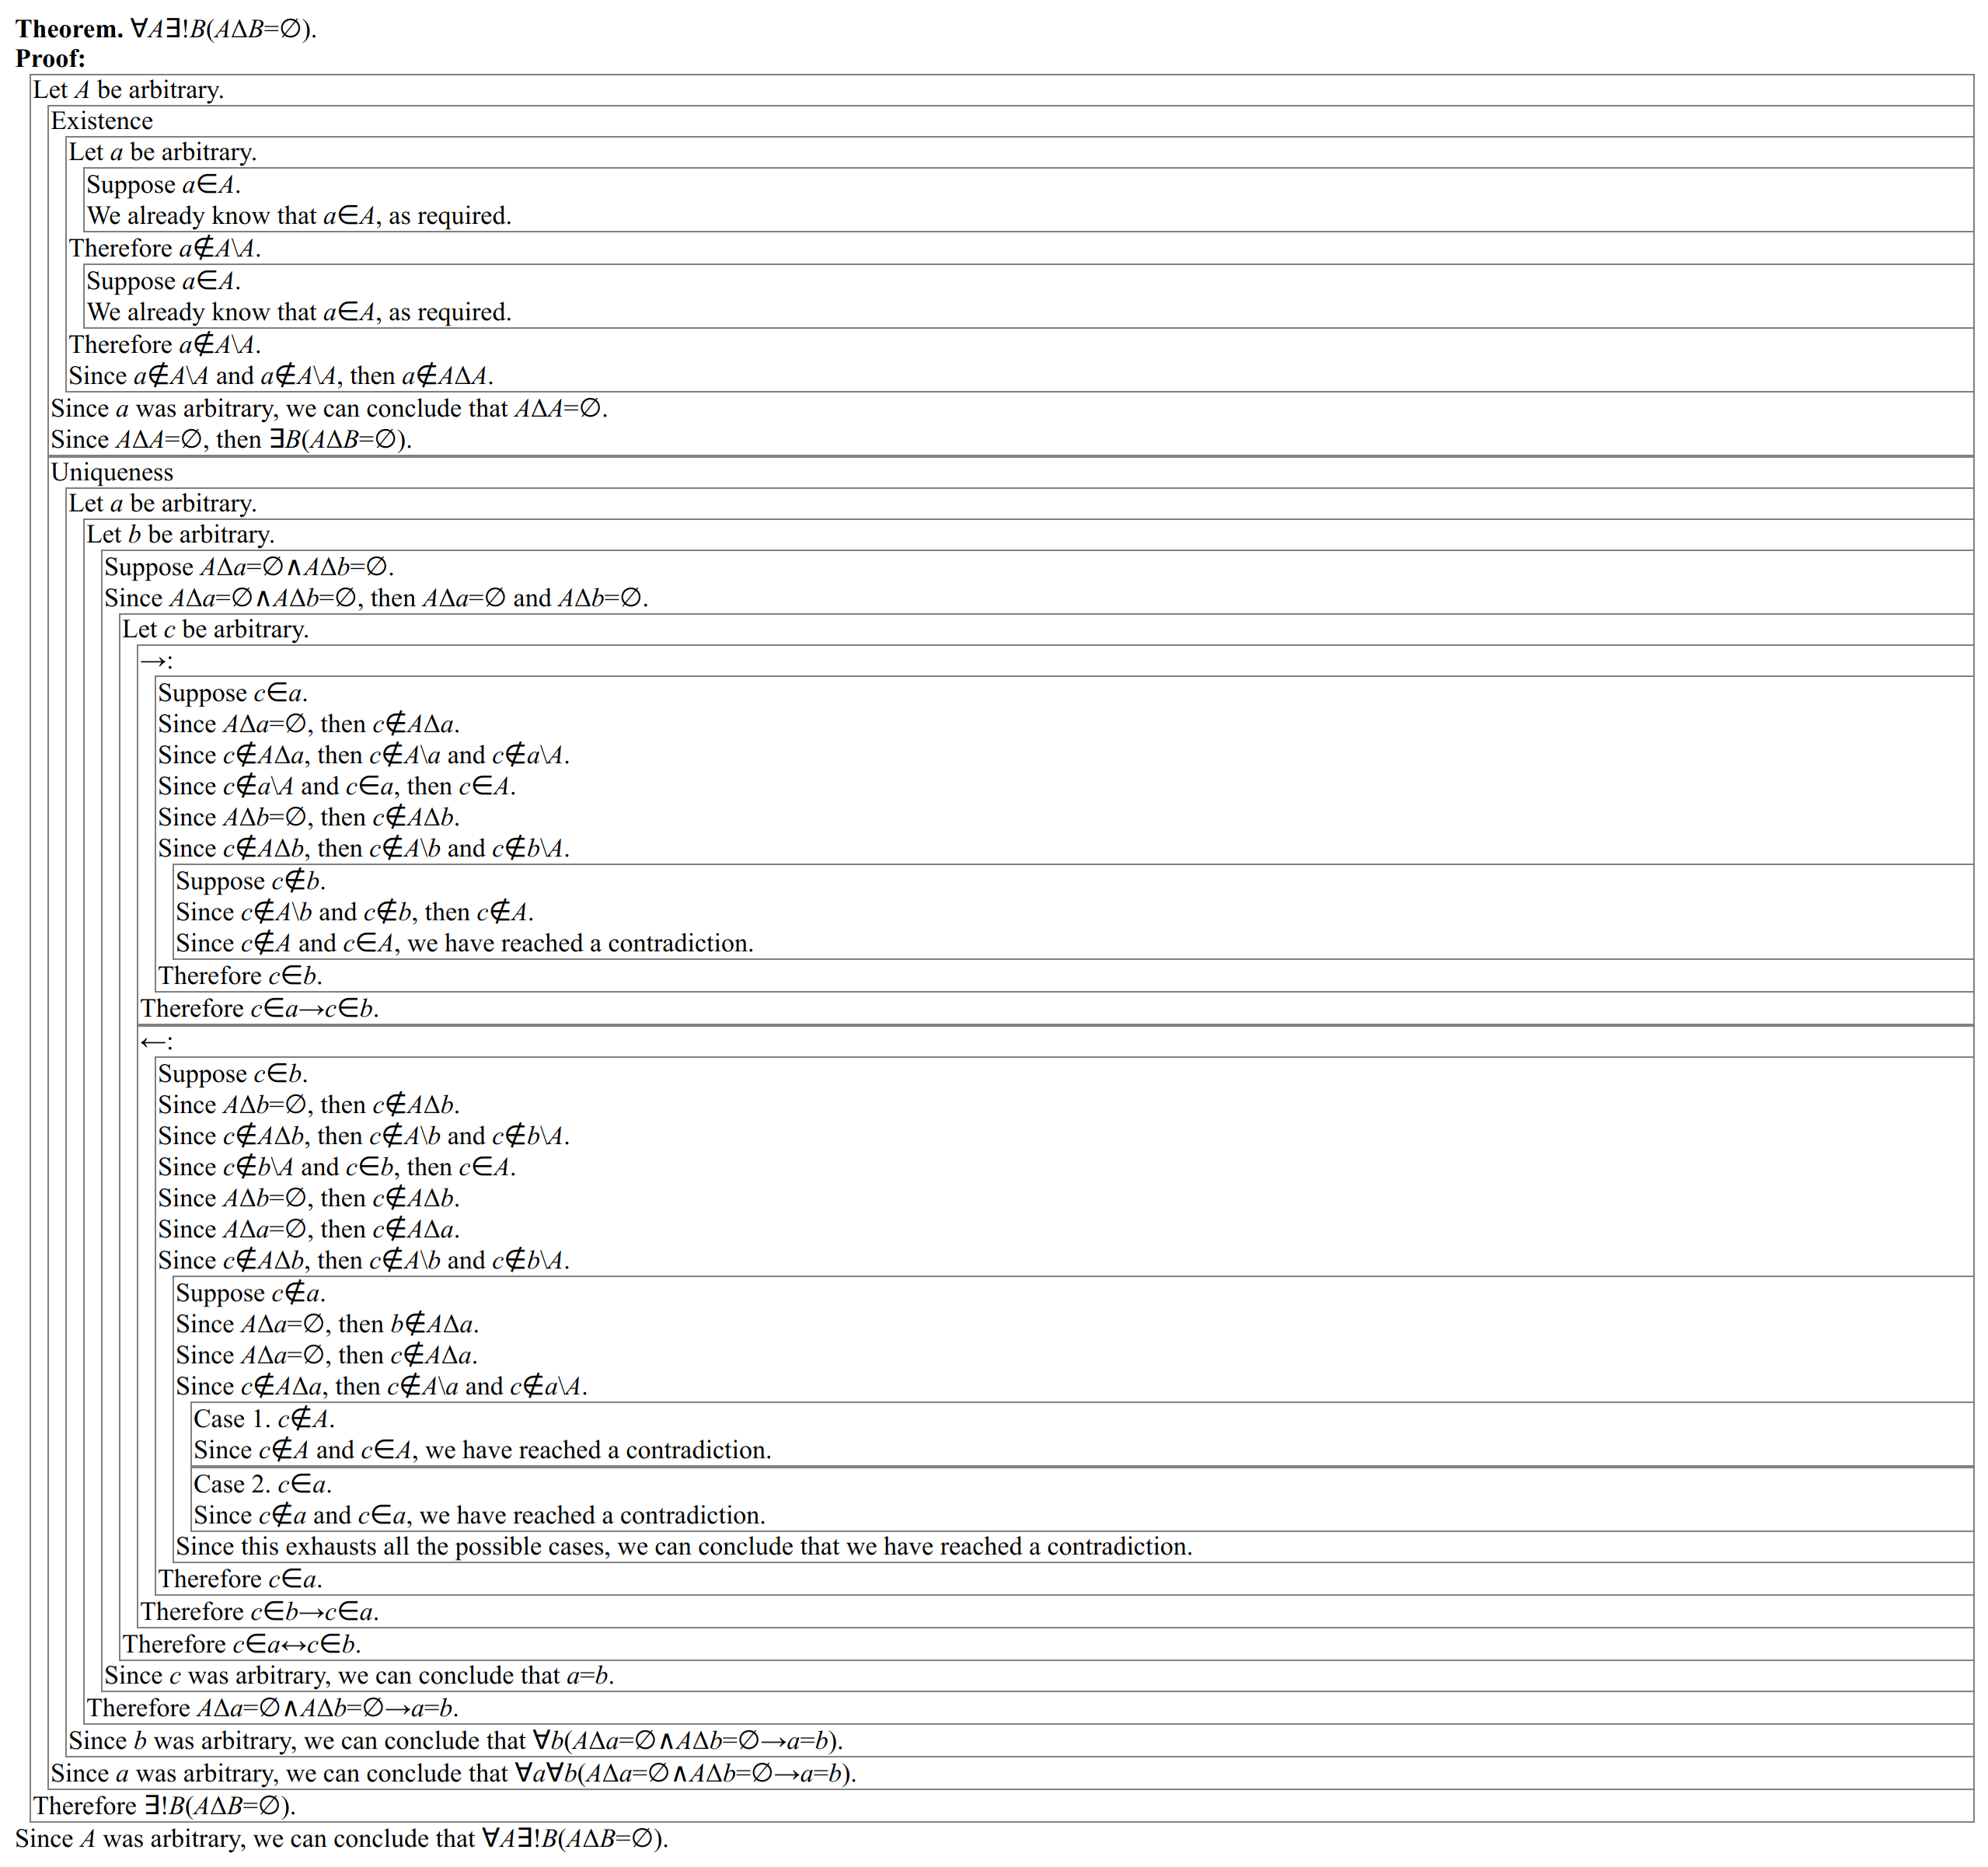
\includegraphics[width=\textwidth,height=\textheight,keepaspectratio]{3_6_9_2}

\vspace{30pt}

(c) $C = A \Delta B$

\textbf{3.6.9.3.pd}
\vspace{10pt}

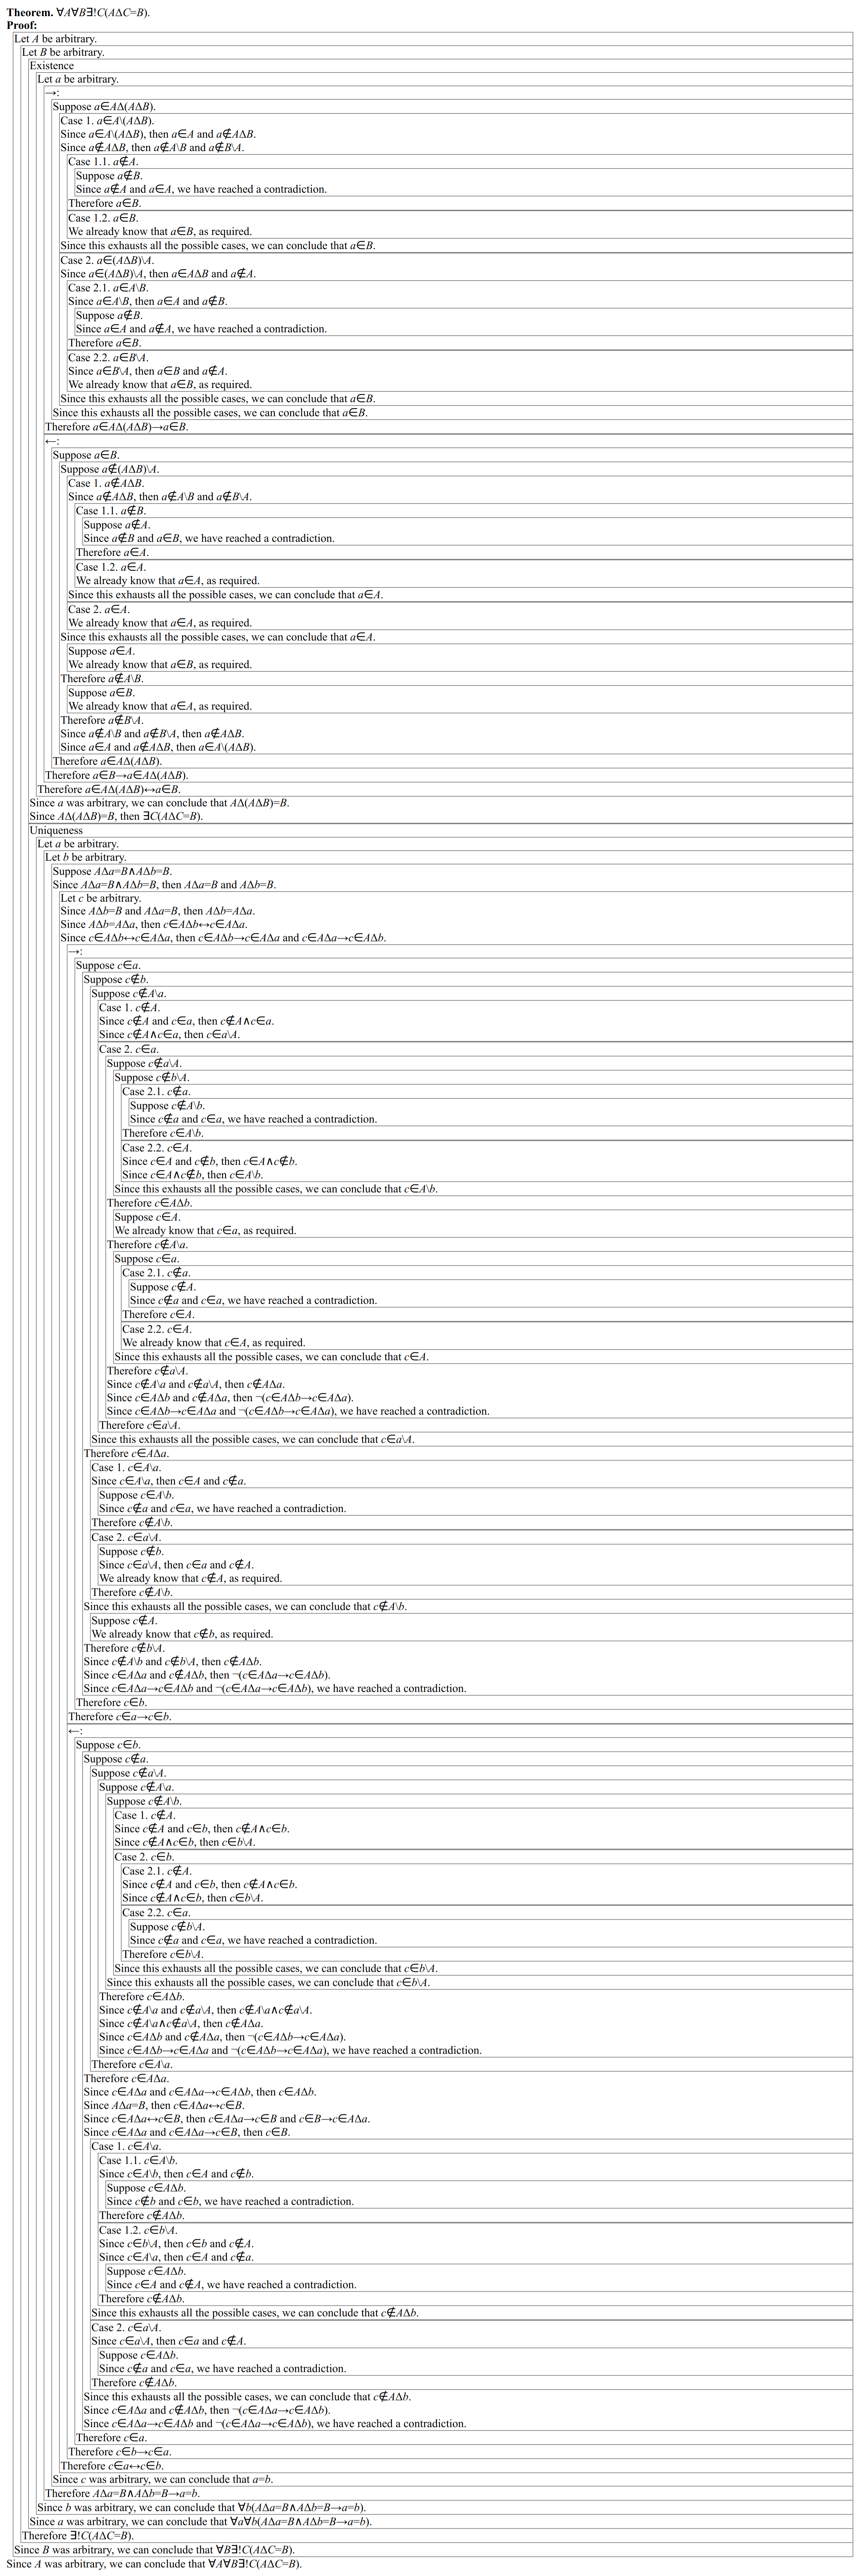
\includegraphics[width=\textwidth,height=\textheight,keepaspectratio]{3_6_9_3}

\vspace{30pt}

(d) $C = A$.

\textbf{3.6.9.4.pd}
\vspace{10pt}

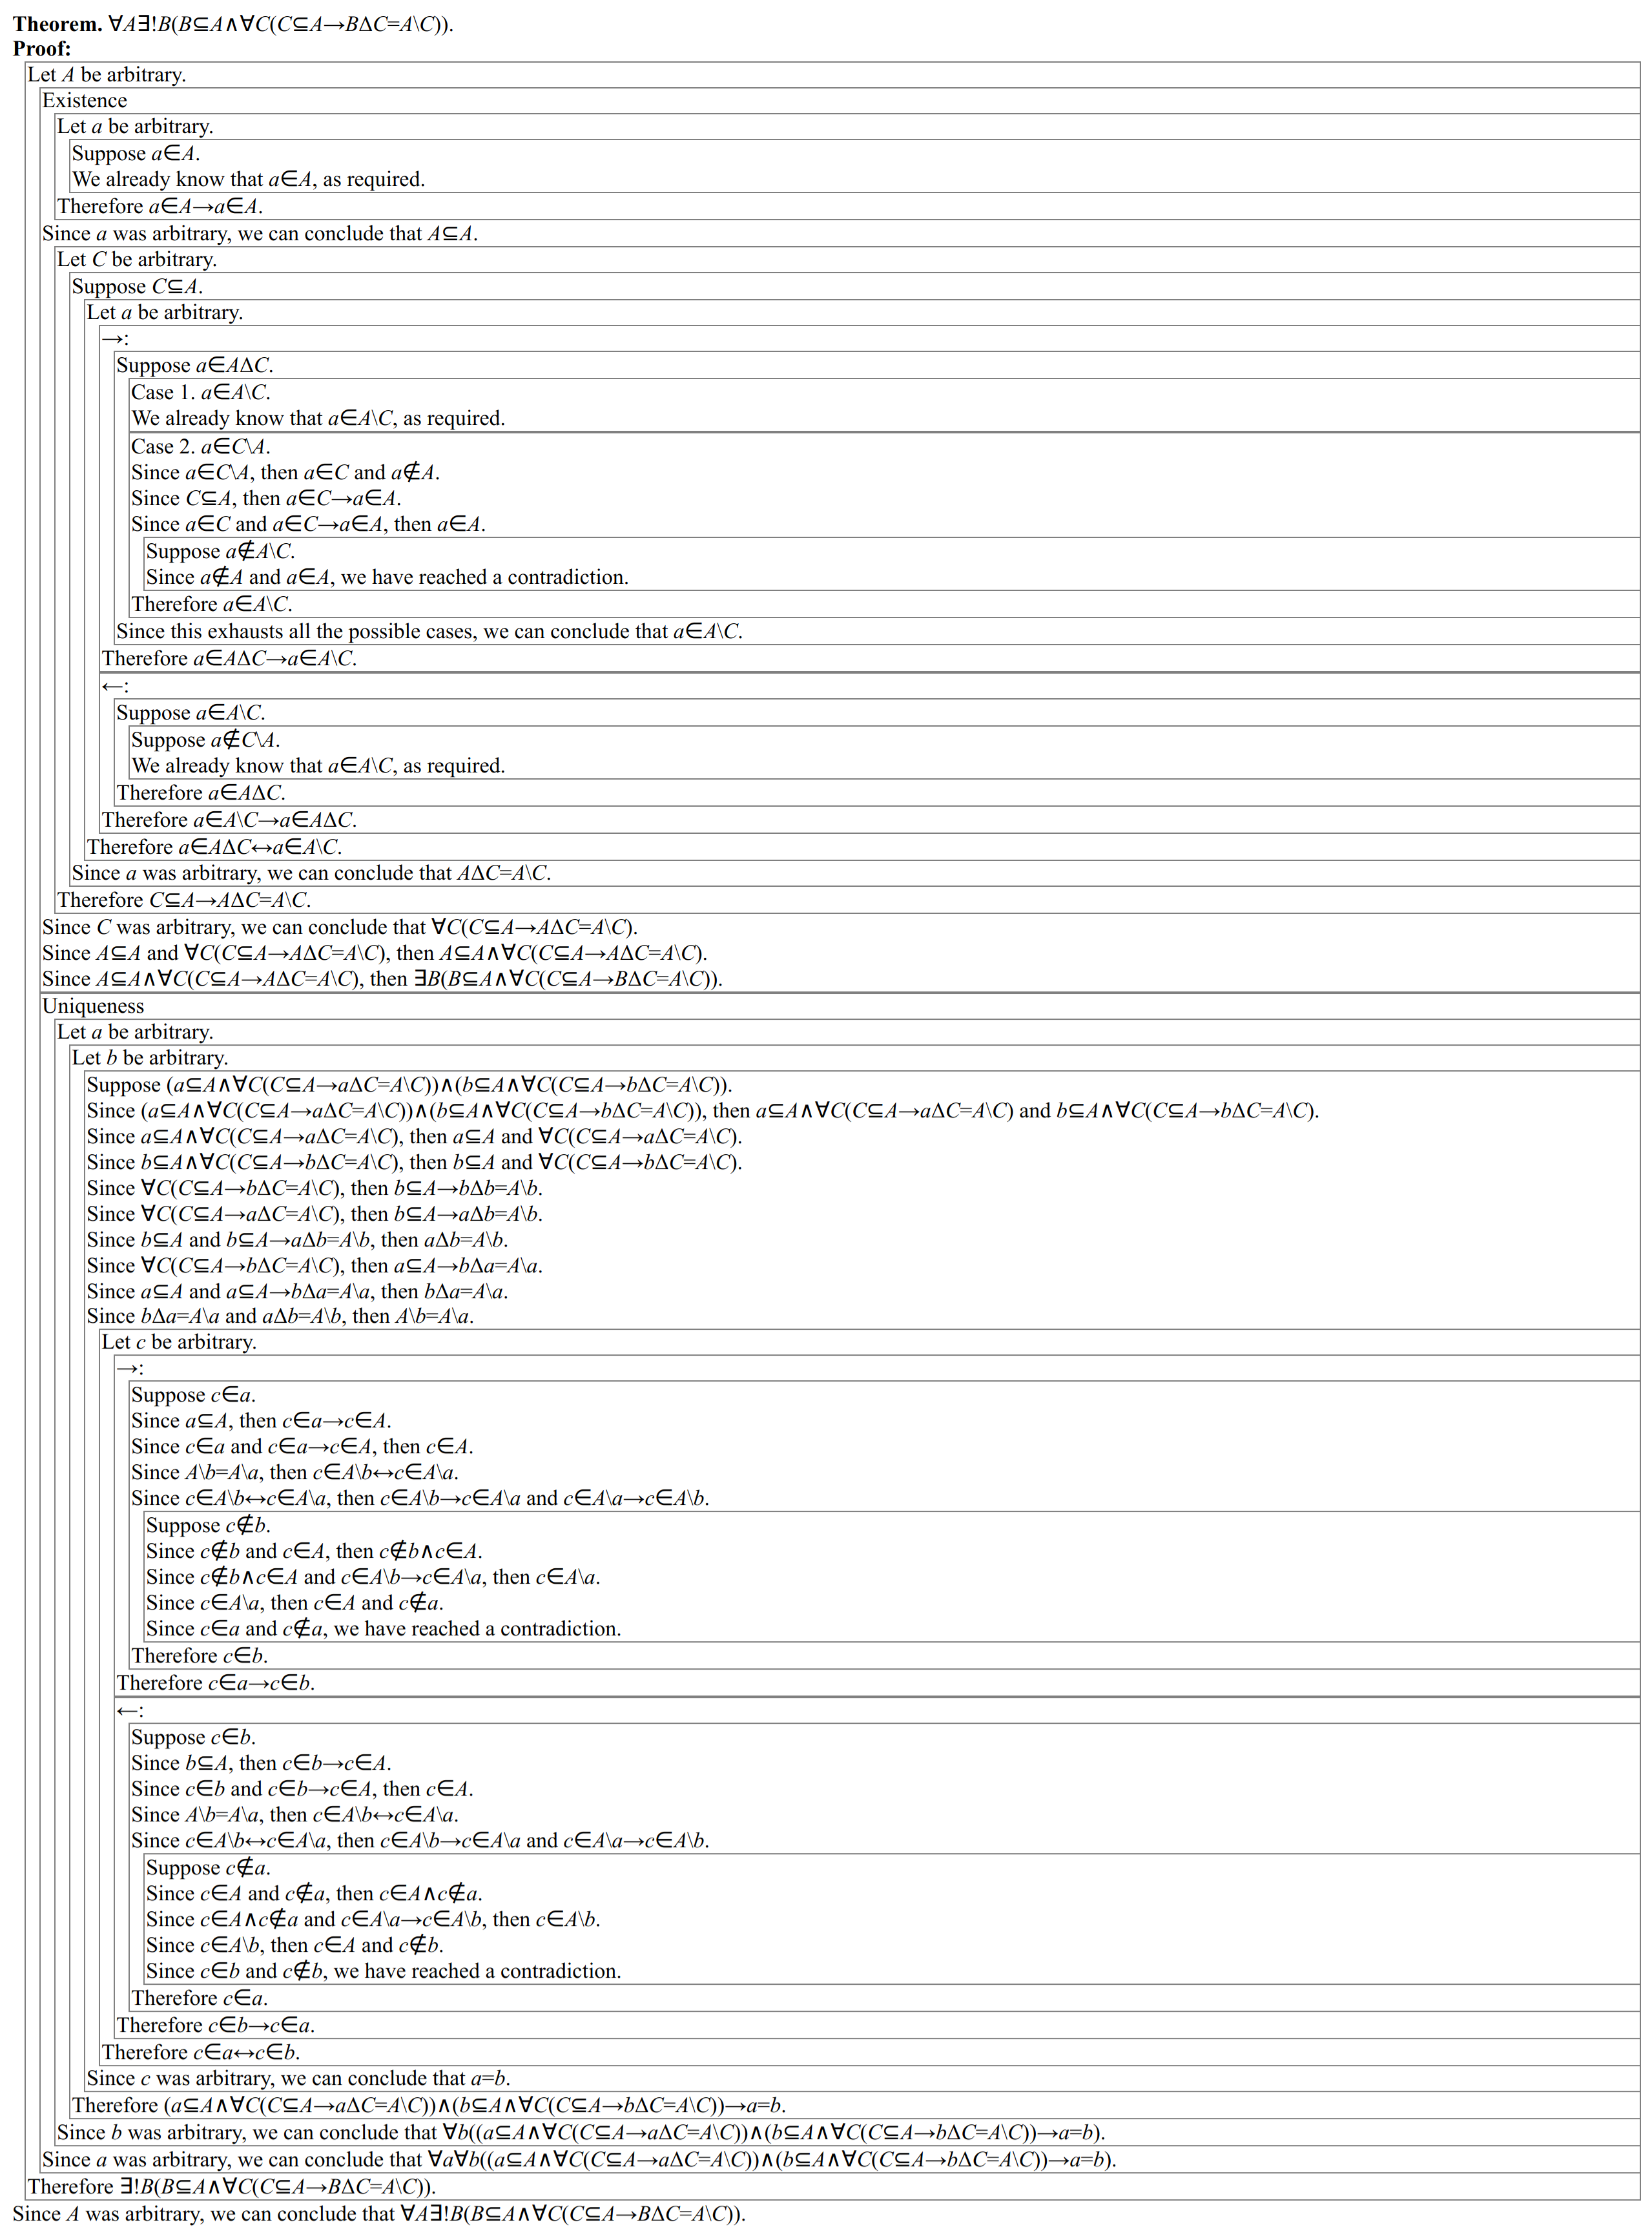
\includegraphics[width=\textwidth,height=\textheight,keepaspectratio]{3_6_9_4}

\vspace{30pt}

$^{\textit{P}}_{\, \textit{D}}$ 10. Suppose A is a set, and for every family of sets $\mathcal{F}$, if $\cup \mathcal{F} = A$ then $A \in \mathcal{F}$. Prove that A has exactly one element. (Hint: For both the existence
and uniqueness parts of the proof, try proof by contradiction.)

\url{https://math.stackexchange.com/q/460296/140585}

\vspace{30pt}

$x = 3$

$A = \{1, 2, 3\}$

$G = \{\{3\}, \{1,2,3\} \setminus \{3\}\} = \{\{3\}, \{1,2\}\}$

$\cup G = \{\{3\}, \{1,2\}\} = \{1,2,3\}$

\vspace{30pt}

$^{\textit{P}}_{\, \textit{D}}$ *11. Suppose $\mathcal{F}$ is a family of sets that has the property that for every $\mathcal{G} \subseteq \mathcal{F}$, $\cup \mathcal{G} \in \mathcal{F}$. Prove that there is a unique set A such that $A \in \mathcal{F}$ and $\forall B \in \mathcal{F}(B \subseteq A)$.


\vspace{30pt}

\textbf{3.6.11.pd}
\vspace{10pt}

\includegraphics[width=\textwidth,height=\textheight,keepaspectratio]{3_6_11}

\vspace{30pt}

\hspace{12pt}12. (a) Suppose P(x) is a statement with a free variable x. Find a formula,
using the logical symbols we have studied, that means "there are
exactly two values of x for which P(x) is true."

\hspace{12pt}(b) Based on your answer to part (a), design a proof strategy for proving
a statement of the form "there are exactly two values of x for which
P(x) is true."

\hspace{12pt}(c) Prove that there are exactly two solutions to the equation $x^3 = x^2$.

(a)

$\exists x \exists y [P(x) \land P(y) \land x \neq y \land \forall z (P(z) \to (z = x) \lor (z = y)]$

\vspace{30pt}

(b)

Let $x = \dots$ and $y = \dots$.

1. Existence of x.

\centerline{
  \begin{tabular}{l l}
  \textit{Givens} & \textit{Goal} \\
    $$ & $P(x)$ \\
 \end{tabular}}
\vspace{10pt}

2. Existence of y.

\centerline{
  \begin{tabular}{l l}
  \textit{Givens} & \textit{Goal} \\
    $$ & $P(y)$ \\
 \end{tabular}}
\vspace{10pt}

3. $x \neq y$

4. Uniqueness of x and y.

\centerline{
  \begin{tabular}{l l}
  \textit{Givens} & \textit{Goal} \\
    $$ & $\forall z (P(z) \to z = x \lor z = y)$ \\
 \end{tabular}}
\vspace{10pt}

\centerline{
  \begin{tabular}{l l}
  \textit{Givens} & \textit{Goal} \\
    $P(z)$ & $z = x \lor z = y$ \\
 \end{tabular}}
\vspace{10pt}

\vspace{30pt}

(c) $x^3 = x^2$

$x^2(x - 1) = 0$

$x_1 = 0$

$x_2 = 1$

\centerline{
  \begin{tabular}{l l}
  \textit{Givens} & \textit{Goal} \\
    $z^3 = z^2$ & $z = 1$ \\
    $z \neq 0$
 \end{tabular}}
\vspace{10pt}

\vspace{20pt}

\textbf{Theorem.} There are exactly two solutions to the equation $x^3 = x^2$.

\textit{Proof.}

Existence of first solution: let $x = 0$. Then,

$x^3 = x^2$

$0 = 0$ which is obviously true.

Existence of second solution: let $y = 1$. Then,

$y^3 = y^2$

$1 = 1$ which is obviously true.

Two solutions are distinct: $x \neq y$

$0 \neq 1$ which is obviously true.

Uniqueness of both solutions:

Suppose $z^3 = z^2$. Suppose $z \neq 0$. Then,

$z^3 = z^2$

Since $z \neq 0$ we can divide both sides by $z^2$, then

$z = 1$

Thus, $z = 1$.


\vspace{50pt}

\textbf{3.7. More Examples of Proofs}

Exercises:


\vspace{30pt}


\vspace{30pt}

$^{\textit{P}}_{\, \textit{D}}$ *1. Suppose $\mathcal{F}$ is a family of sets. Prove that there is a unique set A that has the following two properties:

\hspace{12pt}(a) $\mathcal{F} \subseteq \mathcal{P} (A)$.

\hspace{12pt}(b) $\forall B(\mathcal{F} \subseteq \mathcal{P} (B) \to A \subseteq B)$.
(Hint: First try an example. Let $\mathcal{F} = \{\{1, 2, 3\},\{2, 3, 4\},\{3, 4, 5\}\}$. Can
you find the set A that has properties (a) and (b)?)


\vspace{30pt}

\textbf{3.7.1.pd}
\vspace{10pt}

\includegraphics[width=\textwidth,height=\textheight,keepaspectratio]{3_7_1}

\vspace{30pt}

$A = \cup \mathcal{F} = \{1,2,3,4,5\}$

\vspace{30pt}

$^{\textit{P}}_{\, \textit{D}}$ 2. Suppose A and B are sets.What can you prove about $\mathcal{P} (A \setminus B) \setminus (\mathcal{P} (A) \setminus \mathcal{P} (B))$? (No, it's not equal to $\varnothing$. Try some examples and see what you get.)


\vspace{30pt}

$A = \{1\}$

$B = \{2\}$

$A \setminus B = \{1\}$

$\mathcal{P}(A) \setminus (\mathcal{P}(A) \setminus \mathcal{P}(B))$

$\mathcal{P}(\{1\}) \setminus (\mathcal{P}(\{1\}) \setminus \mathcal{P}(\{2\}))$

$\{\varnothing,1\} \setminus \{1\}$

$\{\varnothing\}$

\textbf{3.7.2.pd}
\vspace{10pt}

\includegraphics[width=\textwidth,height=\textheight,keepaspectratio]{3_7_2}

\vspace{30pt}

$^{\textit{P}}_{\, \textit{D}}$ 3. Suppose that A, B, and C are sets. Prove that the following statements
are equivalent:

\hspace{12pt}(a) $(A \Delta C) \cap (B \Delta C) = \varnothing$.

\hspace{12pt}(b) $A \cap B \subseteq C \subseteq A \cup B$.

\hspace{12pt}(c) $A \Delta C \subseteq A \Delta B$.

$(a) \to (b) \land (b) \to (c) \land (c) \to (a)$ 

\textbf{3.7.3.pd}
\vspace{10pt}

\includegraphics[width=\textwidth,height=\textheight,keepaspectratio]{3_7_3}

\vspace{30pt}

*4. Suppose $\{A_i \mid i \in I\}$ is a family of sets. Prove that if $\mathcal{P} (\cup_{i \in I} A_i) \subseteq
\cup_{i \in I} \mathcal{P} (A_i)$, then there is some $i \in I$ such that $\forall  j \in I (A_j \subseteq A_i)$.

\centerline{
  \begin{tabular}{l l}
  \textit{Givens} & \textit{Goal} \\
    $\{A_i \mid i \in I\}$ & $\exists i \in I \forall  j \in I (A_j \subseteq A_i)$ \\
    $\mathcal{P} (\cup_{i \in I} A_i) \subseteq \cup_{i \in I} \mathcal{P} (A_i)$ & \\
 \end{tabular}}
\vspace{10pt}

\centerline{
  \begin{tabular}{l l}
  \textit{Givens} & \textit{Goal} \\
    $\{A_i \mid i \in I\}$ & $\exists i \in I \forall  j \in I (A_j \subseteq A_i)$ \\
    $\cup_{i \in I} A_i \subseteq \cup_{i \in I} A_i$ & \\
 \end{tabular}}
\vspace{10pt}

\centerline{
  \begin{tabular}{l l}
  \textit{Givens} & \textit{Goal} \\
    $\{A_i \mid i \in I\}$ & $\exists i \in I \forall  j \in I (A_j \subseteq A_i)$ \\
    $\cup_{i \in I} A_i \in \mathcal{P}(\cup_{i \in I} A_i)$ & \\
 \end{tabular}}
\vspace{10pt}

\centerline{
  \begin{tabular}{l l}
  \textit{Givens} & \textit{Goal} \\
    $\{A_i \mid i \in I\}$ & $\exists i \in I \forall  j \in I (A_j \subseteq A_i)$ \\
    $\cup_{i \in I} A_i \in \mathcal{P}(\cup_{i \in I} A_i)$ & \\
 \end{tabular}}
\vspace{10pt}

\centerline{
  \begin{tabular}{l l}
  \textit{Givens} & \textit{Goal} \\
    $\{A_i \mid i \in I\}$ & $\exists i \in I \forall  j \in I (A_j \subseteq A_i)$ \\
    $\exists i \in I (\cup_{i \in I} A_i \subseteq A_i)$ & \\
 \end{tabular}}
\vspace{10pt}

\centerline{
  \begin{tabular}{l l}
  \textit{Givens} & \textit{Goal} \\
    $\{A_i \mid i \in I\}$ & $\forall  j \in I (A_j \subseteq A_i)$ \\
    $\cup_{i \in I} A_i \subseteq A_i$ & \\
 \end{tabular}}
\vspace{10pt}

\centerline{
  \begin{tabular}{l l}
  \textit{Givens} & \textit{Goal} \\
    $\{A_i \mid i \in I\}$ & $\forall  j \in I (A_j \subseteq A_i)$ \\
    $\cup_{i \in I} A_i \subseteq A_i$ & \\
 \end{tabular}}
\vspace{10pt}

\centerline{
  \begin{tabular}{l l}
  \textit{Givens} & \textit{Goal} \\
    $\{A_i \mid i \in I\}$ & $A_j \subseteq A_i$ \\
    $\cup_{i \in I} A_i \subseteq A_i$ & \\
 \end{tabular}}
\vspace{10pt}

$A_j \subseteq \cup_{i \in I} A_i \implies A_j \subseteq A_i$
\vspace{30pt}

\textbf{Theorem.} Suppose $\{A_i \mid i \in I\}$ is a family of sets. If $\mathcal{P} (\cup_{i \in I} A_i) \subseteq \cup_{i \in I} \mathcal{P} (A_i)$, then there is some $i \in I$ such that $\forall  j \in I (A_j \subseteq A_i)$.

\textit{Proof.} Suppose $\mathcal{P} (\cup_{i \in I} A_i) \subseteq \cup_{i \in I} \mathcal{P} (A_i)$. Clearly
$\cup_{i \in I} A_i \subseteq \cup_{i \in I} A_i$, so $\cup_{i \in I} A_i \in \mathcal{P}(\cup_{i \in I} A_i)$ and therefore $\cup_{i \in I} A_i \in \cup_{i \in I} \mathcal{P}(A_i)$. By the definition of the union of a family, we have some $i \in I$ such that $\cup_{i \in I} A_i \subseteq A_i$. Now let $j \in I$ be arbitrary. Then it's not hard to see that $A_j \subseteq \cup_{i \in I}A_i$, so $A_j \subseteq A_i$.

\vspace{30pt}

5. Suppose $\mathcal{F}$ is a nonempty family of sets. Let $I = \cup \mathcal{F}$ and $J = \cap \mathcal{F}$.
Suppose also that $J \neq \varnothing$, and notice that it follows that for every $X \in \mathcal{F}$,
$X \neq \varnothing$, and also that $I \neq \varnothing$. Finally, suppose that $\{A_i \mid i \in I\}$ is an
indexed family of sets.

\hspace{12pt}(a) Prove that $\cup_{i \in I} A_i = \cup_{X \in \mathcal{F}} (\cup_{i \in X} A_i)$.

\hspace{12pt}(b) Prove that $\cap_{i \in I} A_i = \cap_{X \in \mathcal{F}} (\cap_{i \in X} A_i)$.

\hspace{12pt}(c) Prove that $\cup_{i \in J} A_i \subseteq \cap_{X \in \mathcal{F}} (\cup_{i \in X} A_i)$. Is it always true that $\cup_{i \in J} A_i = \cap_{X \in \mathcal{F}} (\cup_{i \in X} A_i)$? Give either a proof or a counterexample to justify
your answer.

\hspace{12pt}(d) Discover and prove a theorem relating $\cap_{i \in J} A_i$ and $\cup_{X \in \mathcal{F}} (\cap_{i \in X} A_i)$.

\vspace{30pt}

(a)

\centerline{
  \begin{tabular}{l l}
  \textit{Givens} & \textit{Goal} \\
    $$ & $\cup_{i \in I} A_i = \cup_{X \in \mathcal{F}} (\cup_{i \in X} A_i)$ \\
 \end{tabular}}
\vspace{10pt}

($\rightarrow$)

\centerline{
  \begin{tabular}{l l}
  \textit{Givens} & \textit{Goal} \\
    $Y \in \cup_{i \in I} A_i$ & $Y \in \cup_{X \in \mathcal{F}} (\cup_{i \in X} A_i)$ \\
    $I = \cup \mathcal{F}$ & $$ \\
    $J = \cap \mathcal{F}$ & $$ \\
    $\{A_i \mid i \in I\}$ & \\
 \end{tabular}}
\vspace{10pt}

$Y \in \cup_{X \in \mathcal{F}} (\cup_{i \in X} A_i)$

$\exists X \in \mathcal{F} (Y \in \cup_{i \in X} A_i)$

$\exists X \in \mathcal{F} \exists i \in X (Y \in A_i)$

$\exists X \exists i (X \in \mathcal{F} \land i \in X \land Y \in A_i)$
\vspace{10pt}

$Y \in \cup_{i \in I} A_i$

$\exists i (i \in I \land Y \in A_i)$

\vspace{10pt}

\centerline{
  \begin{tabular}{l l}
  \textit{Givens} & \textit{Goal} \\
    $\exists i (i \in I \land Y \in A_i)$ & $\exists X \exists i (X \in \mathcal{F} \land i \in X \land Y \in A_i)$ \\
    $I = \cup \mathcal{F}$ & $$ \\
    $J = \cap \mathcal{F}$ & $$ \\
    $\{A_i \mid i \in I\}$ & \\
 \end{tabular}}
\vspace{10pt}

\centerline{
  \begin{tabular}{l l}
  \textit{Givens} & \textit{Goal} \\
    $\exists i (i \in I \land Y \in A_i)$ & $\exists X \exists i (X \in \mathcal{F} \land i \in X \land Y \in A_i)$ \\
    $I = \cup \mathcal{F}$ & $$ \\
    $J = \cap \mathcal{F}$ & $$ \\
    $\{A_i \mid i \in I\}$ & \\
 \end{tabular}}
\vspace{10pt}

$I = \cup \mathcal{F}$

$\forall Z (Z \in I \leftrightarrow Z \in \cup \mathcal{F})$

$\forall Z (Z \in I \leftrightarrow \exists A(A \in \mathcal{F} \land Z \in A))$

\centerline{
  \begin{tabular}{l l}
  \textit{Givens} & \textit{Goal} \\
    $z \in I \land Y \in A_z$ & $\exists X \exists i (X \in \mathcal{F} \land i \in X \land Y \in A_i)$ \\
    $W \in \mathcal{F} \land z \in W$ & $$ \\
 \end{tabular}}
\vspace{10pt}

\centerline{
  \begin{tabular}{l l}
  \textit{Givens} & \textit{Goal} \\
    $W \in \mathcal{F} \land z \in W \land Y \in A_z$ & $\exists X \exists i (X \in \mathcal{F} \land i \in X \land Y \in A_i)$ \\
 \end{tabular}}
\vspace{10pt}

\vspace{20pt}

($\leftarrow$)

\centerline{
  \begin{tabular}{l l}
  \textit{Givens} & \textit{Goal} \\
    $Y \in \cup_{X \in \mathcal{F}} (\cup_{i \in X} A_i)$ & $Y \in \cup_{i \in I} A_i$ \\
    $I = \cup \mathcal{F}$ & $$ \\
    $J = \cap \mathcal{F}$ & $$ \\
    $\{A_i \mid i \in I\}$ & \\
 \end{tabular}}
\vspace{10pt}

\centerline{
  \begin{tabular}{l l}
  \textit{Givens} & \textit{Goal} \\
    $\exists X \exists i (X \in \mathcal{F} \land i \in X \land Y \in A_i)$ & $\exists i (i \in I \land Y \in A_i)$ \\
    $I = \cup \mathcal{F}$ & $$ \\
    $J = \cap \mathcal{F}$ & $$ \\
    $\{A_i \mid i \in I\}$ & \\
 \end{tabular}}
\vspace{10pt}

$Y \in \cup_{X \in \mathcal{F}} (\cup_{i \in X} A_i)$

$\exists X \exists i (X \in \mathcal{F} \land i \in X \land Y \in A_i)$

$W \in \mathcal{F} \land z \in W \land Y \in A_z$

$\forall Z (Z \in I \leftrightarrow \exists A(A \in \mathcal{F} \land Z \in A))$

$\exists A(A \in \mathcal{F} \land z \in A)) \to z \in I$

\centerline{
  \begin{tabular}{l l}
  \textit{Givens} & \textit{Goal} \\
    $z \in I \land Y \in A_z$ & $\exists i (i \in I \land Y \in A_i)$ \\
 \end{tabular}}
\vspace{10pt}

\textbf{Theorem.} $\cup_{i \in I} A_i = \cup_{X \in \mathcal{F}} (\cup_{i \in X} A_i)$.

\textbf{Proof.} Let Y be an arbitrary. Suppose $Y \in \cup_{i \in I} A_i$. Then we can choose some z such that $z \in I$ and $Y \in A_z$. Since $z \in I$ and $I = \cup \mathcal{F}$ we can choose some W such that $W \in \mathcal{F}$ and $z \in W$. Since $W \in \mathcal{F}$ and $z \in W$, and $Y \in A_z$ we can conclude that $Y \in \cup_{X \in \mathcal{F}} (\cup_{i \in X} A_i)$.

Now suppose $Y \in \cup_{X \in \mathcal{F}} (\cup_{i \in X} A_i)$. Then we can choose some W and z such that $W \in \mathcal{F}$ and $z \in W$ and $Y \in A_z$. Since $W \in \mathcal{F}$ and $z \in W$ and $I = \cup \mathcal{F}$, $z \in I$. Since $z \in I$ and $Y \in A_z$ we can conclude that $Y \in \cup_{i \in I} A_i$.

Since Y was an arbitrary, $\forall Y (Y \in \cup_{i \in I} A_i \leftrightarrow Y \in \cup_{X \in \mathcal{F}} (\cup_{i \in X} A_i))$. Thus $\cup_{i \in I} A_i = \cup_{X \in \mathcal{F}} (\cup_{i \in X} A_i)$.

\vspace{30pt}

(b)

$(\rightarrow)$

\centerline{
  \begin{tabular}{l l}
  \textit{Givens} & \textit{Goal} \\
    $Y \in \cap_{i \in I} A_i$ & $Y \in \cap_{X \in \mathcal{F}} (\cap_{i \in X} A_i)$ \\
 \end{tabular}}
\vspace{10pt}

\centerline{
  \begin{tabular}{l l}
  \textit{Givens} & \textit{Goal} \\
    $\forall i (i \in I \to Y \in A_i)$ & $\forall X(X \in \mathcal{F} \to \forall i (i \in X \to Y \in A_i))$ \\
 \end{tabular}}
\vspace{10pt}

\centerline{
  \begin{tabular}{l l}
  \textit{Givens} & \textit{Goal} \\
    $\forall i (i \in I \to Y \in A_i)$ & $Y \in A_i$ \\
    $X \in \mathcal{F}$ & $$ \\
    $i \in X$ & $$ \\
    $I = \cup \mathcal{F}$ & $$ \\
 \end{tabular}}
\vspace{10pt}

\centerline{
  \begin{tabular}{l l}
  \textit{Givens} & \textit{Goal} \\
    $\forall i (i \in I \to Y \in A_i)$ & $Y \in A_i$ \\
    $X \in \mathcal{F}$ & $$ \\
    $i \in X$ & $$ \\
    $\forall Z (Z \in I \leftrightarrow \exists A(A \in \mathcal{F} \land Z \in A))$ & $$ \\
 \end{tabular}}
\vspace{10pt}

$(\leftarrow)$

\centerline{
  \begin{tabular}{l l}
  \textit{Givens} & \textit{Goal} \\
    $Y \in \cap_{X \in \mathcal{F}} (\cap_{i \in X} A_i)$ & $Y \in \cap_{i \in I} A_i$ \\
 \end{tabular}}
\vspace{10pt}

\centerline{
  \begin{tabular}{l l}
  \textit{Givens} & \textit{Goal} \\
    $\forall X(X \in \mathcal{F} \to \forall i (i \in X \to Y \in A_i))$ &  $\forall i (i \in I \to Y \in A_i)$ \\
 \end{tabular}}
\vspace{10pt}

\centerline{
  \begin{tabular}{l l}
  \textit{Givens} & \textit{Goal} \\
    $\forall X(X \in \mathcal{F} \to \forall i (i \in X \to Y \in A_i))$ &  $Y \in A_i$ \\
    $i \in I$ & \\
    $\forall Z (Z \in I \leftrightarrow \exists A(A \in \mathcal{F} \land Z \in A))$ & \\
 \end{tabular}}
\vspace{10pt}

\centerline{
  \begin{tabular}{l l}
  \textit{Givens} & \textit{Goal} \\
    $\forall X(X \in \mathcal{F} \to \forall i (i \in X \to Y \in A_i))$ &  $Y \in A_i$ \\
    $\exists A(A \in \mathcal{F} \land i \in A)$ & \\
 \end{tabular}}
\vspace{10pt}

\centerline{
  \begin{tabular}{l l}
  \textit{Givens} & \textit{Goal} \\
    $M \in \mathcal{F} \to \forall i (i \in M \to Y \in A_i)$ &  $Y \in A_i$ \\
    $M \in \mathcal{F} \land i \in M$ & \\
 \end{tabular}}
\vspace{10pt}

\textbf{Theorem.} $\cap_{i \in I} A_i = \cap_{X \in \mathcal{F}} (\cap_{i \in X} A_i)$

\textit{Proof.} Let Y be an arbitrary. Suppose $Y \in \cap_{i \in I} A_i$.
Let X be arbitrary.
Suppose $X \in \mathcal{F}$.
Let i be arbitrary.
Suppose $i \in X$.
Since $i \in X$ and $X \in \mathcal{F}$ and $I = \cup \mathcal{F}$, in particular we can conclude $i \in I$.
Since $i \in I$ and $Y \in \cap_{i \in I} A_i$, we can conclude $Y \in A_i$.
Thus $Y \in A_i$.
Thus $Y \in \cap_{X \in \mathcal{F}} (\cap_{i \in X} A_i)$.

Now suppose $Y \in \cap_{X \in \mathcal{F}} (\cap_{i \in X} A_i)$.
Let i be an arbitrary.
Suppose $i \in I$.
Since $i \in I$ and $I = \cup \mathcal{F}$ we can choose some X such that $X \in \mathcal{F}$ and $i \in X$.
Since $X \in \mathcal{F}$ and $i \in X$, $Y \in A_i$.
Thus $Y \in A_i$
Thus $Y \in \cap_{i \in I} A_i$

Therefore $\cap_{i \in I} A_i = \cap_{X \in \mathcal{F}} (\cap_{i \in X} A_i)$.


\vspace{30pt}

(c)

\centerline{
  \begin{tabular}{l l}
  \textit{Givens} & \textit{Goal} \\
    $$ & $\forall Y (Y \in \cup_{i \in J} A_i \to Y \in \cap_{X \in \mathcal{F}} (\cup_{i \in X} A_i))$ \\
 \end{tabular}}
\vspace{10pt}

\centerline{
  \begin{tabular}{l l}
  \textit{Givens} & \textit{Goal} \\
    $Y \in \cup_{i \in J} A_i$ & $Y \in \cap_{X \in \mathcal{F}} (\cup_{i \in X} A_i)$ \\
 \end{tabular}}
\vspace{10pt}

$\forall X (X \in \mathcal{F} \to \exists i (i \in X \land Y \in A_i)$

\centerline{
  \begin{tabular}{l l}
  \textit{Givens} & \textit{Goal} \\
    $Y \in \cup_{i \in J} A_i$ & $\exists i (i \in X \land Y \in A_i)$ \\
    $X \in \mathcal{F}$ & \\
 \end{tabular}}
\vspace{10pt}

\centerline{
  \begin{tabular}{l l}
  \textit{Givens} & \textit{Goal} \\
    $z \in J \land Y \in A_z$ & $\exists i (i \in X \land Y \in A_i)$ \\
    $X \in \mathcal{F}$ & \\
    $J = \cap \mathcal{F}$ & \\
 \end{tabular}}
\vspace{10pt}

$\forall Z (Z \in J \to Z \in \cap \mathcal{F})$

$\forall Z (Z \in J \to \forall W (W \in \mathcal{F} \to Z \in W))$

$z \in J \to \forall W (W \in \mathcal{F} \to Z \in W))$

$\forall W (W \in \mathcal{F} \to z \in W))$

$X \in \mathcal{F} \to z \in X$
\vspace{20pt}

\textbf{Theorem.} $\cup_{i \in J} A_i \subseteq \cap_{X \in \mathcal{F}} (\cup_{i \in X} A_i)$.

\textit{Proof.} Let Y be arbitrary. Suppose $Y \in \cup_{i \in J} A_i$. Suppose $X \in \mathcal{F}$. Since $Y \in \cup_{i \in J} A_i$ we can choose some z such that $z \in J$ and $Y \in A_z$. Since $X \in F$ and $J = \cap \mathcal{F}$ and $z \in J$ we can conclude $z \in X$. Thus, $Y \in \cap_{X \in \mathcal{F}} (\cup_{i \in X} A_i)$. Therefore, $\cup_{i \in J} A_i \subseteq \cap_{X \in \mathcal{F}} (\cup_{i \in X} A_i)$.

\vspace{30pt}

$\cup_{i \in J} A_i = \cap_{X \in \mathcal{F}} (\cup_{i \in X} A_i)$

\centerline{
  \begin{tabular}{l l}
  \textit{Givens} & \textit{Goal} \\
    $Y \in \cap_{X \in \mathcal{F}} (\cup_{i \in X} A_i)$ & $Y \in \cup_{i \in J} A_i$ \\
 \end{tabular}}
\vspace{10pt}

\centerline{
  \begin{tabular}{l l}
  \textit{Givens} & \textit{Goal} \\
    $\forall (X \in \mathcal{F} \to \exists i (i \in X \land Y \in A_i)$ & $Y \in \cup_{i \in J} A_i$ \\
    $\forall Z (Z \in J \to \forall W (W \in \mathcal{F} \to Z \in W))$ & $$ \\
 \end{tabular}}
\vspace{10pt}

\centerline{
  \begin{tabular}{l l}
  \textit{Givens} & \textit{Goal} \\
    $\forall X(X \in \mathcal{F} \to \exists i (i \in X \land Y \in A_i)$ & $\exists i (i \in J \land Y \in A_i)$ \\
    $\forall Z (Z \in J \leftrightarrow \forall W (W \in \mathcal{F} \to Z \in W))$ & $$ \\
 \end{tabular}}
\vspace{10pt}

$\cup_{i \in J} A_i = \cap_{X \in \mathcal{F}} (\cup_{i \in X} A_i)$

$J = \{1\}$

$\mathcal{F} = \{\{1,2\}, \{1,2\}, \{1,3\} \}$

$A_1 = \{1,2\}$

$A_2 = \{3\}$

$A_3 = \{3\}$

$\cup_{i \in J} A_i = \{1,2\}$

$X = \{1,2\}$

$\cup_{i \in X} A_i = \{1,2,3\}$

$X = \{1,2\}$

$\cup_{i \in X} A_i = \{1,2,3\}$

$X = \{1,3\}$

$\cup_{i \in X} A_i = \{1,2,3\}$

$\cap_{X \in \mathcal{F}} (\cup_{i \in X} A_i) = \{1,2,3\}$

$\{1,2\} \neq \{1,2,3\}$

\vspace{30pt}

(d)

$\cup_{X \in \mathcal{F}} (\cap_{i \in X} A_i) \subseteq \cap_{i \in J} A_i$.

\centerline{
  \begin{tabular}{l l}
    \textit{Givens} & \textit{Goal} \\
    $Y \in \cup_{X \in \mathcal{F}} (\cap_{i \in X} A_i)$ & $Y \in \cap_{i \in J} A_i$  \\
 \end{tabular}}
\vspace{10pt}

\centerline{
  \begin{tabular}{l l}
    \textit{Givens} & \textit{Goal} \\
    $\exists X (X \in \mathcal{F} \land \forall i (i \in X \to Y \in A_i))$ & $\forall i (i \in J \to Y \in A_i)$  \\
 \end{tabular}}
\vspace{10pt}

\centerline{
  \begin{tabular}{l l}
    \textit{Givens} & \textit{Goal} \\
    $\forall i (i \in B \to Y \in A_i)$ & $Y \in A_i$  \\
    $i \in J$ & \\
    $i \in B$ & \\
 \end{tabular}}
\vspace{10pt}

$\forall Z (Z \in J \leftrightarrow \forall T (T \in \mathcal{F} \to Z \in T))$.

\textbf{Theorem.} $\cup_{X \in \mathcal{F}} (\cap_{i \in X} A_i) \subseteq \cap_{i \in J} A_i$

\textit{Proof.} Let Y be an arbitrary. Suppose $Y \in \cup_{X \in \mathcal{F}} (\cap_{i \in X} A_i)$. Suppose $i \in J$. Since $Y \in \cup_{X \in \mathcal{F}} (\cap_{i \in X} A_i)$ we can choose some B such that $B \in \mathcal{F}$ and $Y \in \cap_{i \in X}A_i$. Since $i \in J$ and $J = \cap \mathcal{F}$, $i \in \cap \mathcal{F}$. Since $B \in \mathcal{F}$ and $i \in \cap \mathcal{F}$, $i \in B$. Since $i \in B$ and $Y \in \cap_{i \in X}A_i$, $Y \in A_i$. Thus, $Y \in \cap_{i \in J} A_i$. Therefore, $\cup_{X \in \mathcal{F}} (\cap_{i \in X} A_i) \subseteq \cap_{i \in J} A_i$.

\vspace{30pt}

$\cup_{X \in \mathcal{F}} (\cap_{i \in X} A_i) = \cap_{i \in J} A_i$

$J = \cap \mathcal{F}$

$J = \{1\}$

$\mathcal{F} = \{\{1,2\}, \{1,2\}, \{1,3\} \}$

$A_1 = \{3\}$

$A_2 = \{1,2\}$

$A_3 = \{1,2\}$

$X = \{1,2\}$

$\cap_{i \in X} A_i = \varnothing$

$X = \{1,2\}$

$\cap_{i \in X} A_i = \varnothing$

$X = \{1,3\}$

$\cap_{i \in X} A_i = \varnothing$

$\cup_{X \in \mathcal{F}} (\cap_{i \in X} A_i) = \varnothing$

$\cap_{i \in J} A_i = {3}$

${3} \neq \varnothing$

\vspace{30pt}

6. Prove that $\displaystyle{\lim_{x \to 2} \frac{3x^2-12}{x-2} = 12}$.

\vspace{30pt}

$\forall \varepsilon > 0 \exists \delta > 0 \forall x (0 < |x - 2| < \delta \to |\frac{3x^2-12}{x-2} - 12| < \varepsilon)$

Let $\varepsilon$ be an arbitrary positive number.

$\exists \delta > 0 \forall x (0 < |x - 2| < \delta \to |\frac{3x^2-12}{x-2} - 12| < \varepsilon)$


\centerline{
  \begin{tabular}{l l}
    \textit{Givens} & \textit{Goal} \\
    $\varepsilon > 0$ & $|\frac{3x^2-12}{x-2} - 12| < \varepsilon$  \\
    $\delta = (\text{some positive number})$ & $$ \\
    $0 < |x - 2| < \delta$ & $$ \\
 \end{tabular}}
\vspace{10pt}

$0 < |x - 2|$, so $x \neq 2$

$|\frac{3x^2-12}{x-2} - 12| < \varepsilon$

$|\frac{3(x - 2)(x + 2)}{x-2} - 12| < \varepsilon$

$|3(x + 2) - 12| < \varepsilon$

$3|x - 2| < \varepsilon$

$|x - 2| < \delta$, so $3|x - 2| < 3 \delta$

$3 \delta = \varepsilon$

$\delta = \varepsilon/3$

\textbf{Theorem.} $\displaystyle{\lim_{x \to 2} \frac{3x^2-12}{x-2} = 12}$.

\textit{Proof.} Supppose $\varepsilon > 0$. Let $\delta = \varepsilon/3$, which is also clearly positive. Let x be an arbitrary real number, and suppose that $0 < |x - 2| < \delta$. Then

$|\frac{3x^2-12}{x-2} - 12|$

$= |\frac{3(x - 2)(x + 2)}{x-2} - 12|$

$= |3(x + 2) - 12|$

$= 3|x - 2| < \delta$

$= 3 (\frac{\varepsilon}{3}) = \varepsilon $

\vspace{30pt}

*7. Prove that if $\displaystyle{\lim_{x \to c} f (x) = L}$ and $L > 0$, then there is some number $\delta > 0$
such that for all x, if $0 < |x - c| < \delta$ then $f (x) > 0$.

\vspace{30pt}

\centerline{
  \begin{tabular}{l l}
    \textit{Givens} & \textit{Goal} \\
    $\displaystyle{\lim_{x \to c} f (x) = L}$ & $\exists \delta > 0 \forall x (0 < |x - c| < \delta \to f (x) > 0)$  \\
    $L > 0$ & \\
 \end{tabular}}
\vspace{10pt}

$\displaystyle{\lim_{x \to c} f (x) = L} \implies$

$\forall \varepsilon > 0 \exists \delta > 0 \forall x(0 < |x - c| < \delta \to |f(x) - L| < \varepsilon)$

\centerline{
  \begin{tabular}{l l}
    \textit{Givens} & \textit{Goal} \\
    $\forall \varepsilon > 0 \exists \delta > 0 \forall x(0 < |x - c| < \delta \to |f(x) - L| < \varepsilon)$ & $\exists \delta > 0 \forall x (0 < |x - c| < \delta \to f (x) > 0)$ \\
    $L > 0$ & $$ \\
 \end{tabular}}
\vspace{10pt}

\centerline{
  \begin{tabular}{l l}
    \textit{Givens} & \textit{Goal} \\
    $\forall \varepsilon > 0 \exists \delta > 0 \forall x(0 < |x - c| < \delta \to |f(x) - L| < \varepsilon)$ & $\forall x (0 < |x - c| < \delta \to f (x) > 0)$ \\
    $L > 0$ & \\
    $\delta = (\text{some value})$ & \\
 \end{tabular}}
\vspace{10pt}

\centerline{
  \begin{tabular}{l l}
    \textit{Givens} & \textit{Goal} \\
    $\exists \delta > 0 \forall x(0 < |x - c| < \delta \to |f(x) - L| < L)$ & $f (x) > 0$  \\
    $L > 0$ & \\
    $K > 0$ & \\
    $\varepsilon > 0$ & \\
    $\delta = (\text{some value})$ & \\
    $0 < |x - c| < \delta$ & \\
 \end{tabular}}
\vspace{10pt}

\centerline{
  \begin{tabular}{l l}
    \textit{Givens} & \textit{Goal} \\
    $\forall x(0 < |x - c| < K \to |f(x) - L| < L)$ & $f (x) > 0$  \\
    $L > 0$ & \\
    $\varepsilon > 0$ & \\
    $\delta = K$ & \\
    $0 < |x - c| < \delta$ & \\
 \end{tabular}}
\vspace{10pt}

$|f(x) - L| < L \implies f(x) > 0$

\vspace{30pt}

\textbf{Theorem.} If $\displaystyle{\lim_{x \to c} f (x) = L}$ and $L > 0$, then there is some number $\delta > 0$ such that for all x, if $0 < |x - c| < \delta$ then $f (x) > 0$.

\textit{Proof.} Suppose $\displaystyle{\lim_{x \to c} f (x) = L}$. Let $\varepsilon = L$. Then by definition of limit there is some $\delta > 0$ such that for all x, if $0 < |x - c| < \delta$ then $|f(x) - L| < \varepsilon = L$. But if $|f(x) - L| < L$ then $-L < f(x) - L < L$, so $0 < f(x) < 2L$. Therefore, if $0 < |x - c| < \delta$ then $f(x) > 0$.

\vspace{30pt}

8. Prove that if $\displaystyle{\lim_{x \to c} f (x) = L}$ then $\displaystyle{\lim_{x \to c} 7 f (x) = 7L}$.

\centerline{
  \begin{tabular}{l l}
    \textit{Givens} & \textit{Goal} \\
    $\displaystyle{\lim_{x \to c} f (x) = L}$ & $\displaystyle{\lim_{x \to c} 7 f (x) = 7L}$ \\
 \end{tabular}}
\vspace{10pt}

\centerline{
  \begin{tabular}{l l}
    \textit{Givens} & \textit{Goal} \\
    $\forall \varepsilon > 0 \exists \delta > 0 \forall x (0 < |x - c| < \delta \to |f(x) - L| < \varepsilon)$ & $\forall \varepsilon > 0 \exists \delta > 0 \forall x (0 < |x - c| < \delta \to |7f(x) - 7L| < \varepsilon)$ \\
 \end{tabular}}
\vspace{10pt}

\centerline{
  \begin{tabular}{l l}
    \textit{Givens} & \textit{Goal} \\
    $\forall \varepsilon > 0 \exists \delta > 0 \forall x (0 < |x - c| < \delta \to |f(x) - L| < \varepsilon)$ & $\exists \delta > 0 \forall x (0 < |x - c| < \delta \to |7f(x) - 7L| < \varepsilon)$ \\
    $\varepsilon > 0$ & \\
 \end{tabular}}
\vspace{10pt}

\centerline{
  \begin{tabular}{l l}
    \textit{Givens} & \textit{Goal} \\
    $\forall \varepsilon > 0 \exists \delta > 0 \forall x (0 < |x - c| < \delta \to |f(x) - L| < \varepsilon)$ & $\forall x (0 < |x - c| < \delta \to |7f(x) - 7L| < \varepsilon)$ \\
    $\varepsilon > 0$ & \\
    $\delta = (\text{some value})$ & \\
    $\delta > 0$
 \end{tabular}}
\vspace{10pt}

\centerline{
  \begin{tabular}{l l}
    \textit{Givens} & \textit{Goal} \\
    $\forall \varepsilon > 0 \exists \delta > 0 \forall x (0 < |x - c| < \delta \to |f(x) - L| < \varepsilon)$ & $|7f(x) - 7L| < \varepsilon$ \\
    $\varepsilon > 0$ & \\
    $\delta = (\text{some value})$ & \\
    $\delta > 0$ & \\
    $0 < |x - c| < \delta$ & \\
 \end{tabular}}
\vspace{10pt}

$7|f(x) - L| < \varepsilon \implies |f(x) - L| < \frac{\varepsilon}{7}$

\centerline{
  \begin{tabular}{l l}
    \textit{Givens} & \textit{Goal} \\
    $\forall x (0 < |x - c| < K \to |f(x) - L| < \delta / 7)$ & $|7f(x) - 7L| < \varepsilon$ \\
    $\varepsilon > 0$ & \\
    $K > 0$ & \\
    $\delta = K$ & \\
    $\delta > 0$ & \\
    $\varepsilon = \delta / 7$ & \\
    $0 < |x - c| < \delta$ & \\
 \end{tabular}}
\vspace{10pt}

\centerline{
  \begin{tabular}{l l}
    \textit{Givens} & \textit{Goal} \\
    $|f(x) - L| < \delta / 7$ & $|7f(x) - 7L| < \varepsilon$ \\
    $\varepsilon > 0$ & \\
    $K > 0$ & \\
    $\delta = K$ & \\
    $\delta > 0$ & \\
    $\varepsilon = \delta / 7$ & \\
    $0 < |x - c| < \delta$ & \\
 \end{tabular}}
\vspace{10pt}

\textbf{Theorem.} If $\displaystyle{\lim_{x \to c} f (x) = L}$ then $\displaystyle{\lim_{x \to c} 7 f (x) = 7L}$.


\textit{Proof.} Suppose $\displaystyle{\lim_{x \to c} f (x) = L}$. Let $\varepsilon = \delta / 7$.
Then by definition of limit, there is some $\delta > 0$ such that for all x, if $0 < |x - c| < \varepsilon$ then $|f(x) - L| < \delta / 7$. But if $|f(x) - L| < \delta / 7$ then
$-\delta / 7 < f(x) - L < \delta / 7$, so $-\delta < 7f(x) - 7L < \delta$. Therefore, if $0 < |x - c| < \delta$ then $|7f(x) - 7L| < \delta$.

\vspace{30pt}

*9. Consider the following putative theorem.

\textbf{Theorem.} There are irrational numbers a and b such that $a^b$ is rational.

Is the following proof correct? If so, what proof strategies does it use?
If not, can it be fixed? Is the theorem correct? (Note: The proof uses the
fact that $\sqrt{2}$ is irrational, which we'll prove in Chapter 6.)

\textit{Proof.} Either $\sqrt{2}^{\sqrt{2}}$ is rational or it's irrational.

\textit{Case} 1. $\sqrt{2}^{\sqrt{2}}$ is rational. Let $a = b = \sqrt{2}$. Then a and b are irrational,
and $a^b = \sqrt{2}^{\sqrt{2}}$, which we are assuming in this case is rational.

\textit{Case} 2. $\sqrt{2}^{\sqrt{2}}$ is irrational. Let $a = \sqrt{2}^{\sqrt{2}}$ and $b = \sqrt{2}$. Then a is
irrational by assumption, and we know that b is also irrational. Also,
$a^b = \big(\sqrt{2}^{\sqrt{2}}\big)^{\sqrt{2}} = \sqrt{2}^{(\sqrt{2}*\sqrt{2})} = (\sqrt{2})^2 = 2$, which is rational.

\vspace{30pt}

$\exists a \notin \mathbb{Q} \exists b \notin \mathbb{Q} (ab \in \mathbb{Q})$

Case 1. $\sqrt{2}^{\sqrt{2}}$ is rational.

$\sqrt{2}$ is irrational number

\centerline{
  \begin{tabular}{l l}
    \textit{Givens} & \textit{Goal} \\
    $a = b = \sqrt{2}$ & $$ \\
 \end{tabular}}
\vspace{10pt}

Case 2. $\sqrt{2}^{\sqrt{2}}$ is irrational.

\centerline{
  \begin{tabular}{l l}
    \textit{Givens} & \textit{Goal} \\
    $a = \sqrt{2}^{\sqrt{2}}$ & $$ \\
    $b = \sqrt{2}$ & $$ \\
 \end{tabular}}
\vspace{10pt}

a is irrational by assuming and we now that b is also irrational.

$a^b = \big(\sqrt{2}^{\sqrt{2}}\big)^{\sqrt{2}} = \sqrt{2}^{(\sqrt{2}*\sqrt{2})} = (\sqrt{2})^2 = 2$

Proof is correct.















































\end{document}
